% Options for packages loaded elsewhere
\PassOptionsToPackage{unicode}{hyperref}
\PassOptionsToPackage{hyphens}{url}
\PassOptionsToPackage{dvipsnames,svgnames,x11names}{xcolor}
%
\documentclass[
  letterpaper,
  DIV=11,
  numbers=noendperiod]{scrreprt}

\usepackage{amsmath,amssymb}
\usepackage{iftex}
\ifPDFTeX
  \usepackage[T1]{fontenc}
  \usepackage[utf8]{inputenc}
  \usepackage{textcomp} % provide euro and other symbols
\else % if luatex or xetex
  \usepackage{unicode-math}
  \defaultfontfeatures{Scale=MatchLowercase}
  \defaultfontfeatures[\rmfamily]{Ligatures=TeX,Scale=1}
\fi
\usepackage{lmodern}
\ifPDFTeX\else  
    % xetex/luatex font selection
\fi
% Use upquote if available, for straight quotes in verbatim environments
\IfFileExists{upquote.sty}{\usepackage{upquote}}{}
\IfFileExists{microtype.sty}{% use microtype if available
  \usepackage[]{microtype}
  \UseMicrotypeSet[protrusion]{basicmath} % disable protrusion for tt fonts
}{}
\makeatletter
\@ifundefined{KOMAClassName}{% if non-KOMA class
  \IfFileExists{parskip.sty}{%
    \usepackage{parskip}
  }{% else
    \setlength{\parindent}{0pt}
    \setlength{\parskip}{6pt plus 2pt minus 1pt}}
}{% if KOMA class
  \KOMAoptions{parskip=half}}
\makeatother
\usepackage{xcolor}
\setlength{\emergencystretch}{3em} % prevent overfull lines
\setcounter{secnumdepth}{5}
% Make \paragraph and \subparagraph free-standing
\ifx\paragraph\undefined\else
  \let\oldparagraph\paragraph
  \renewcommand{\paragraph}[1]{\oldparagraph{#1}\mbox{}}
\fi
\ifx\subparagraph\undefined\else
  \let\oldsubparagraph\subparagraph
  \renewcommand{\subparagraph}[1]{\oldsubparagraph{#1}\mbox{}}
\fi

\usepackage{color}
\usepackage{fancyvrb}
\newcommand{\VerbBar}{|}
\newcommand{\VERB}{\Verb[commandchars=\\\{\}]}
\DefineVerbatimEnvironment{Highlighting}{Verbatim}{commandchars=\\\{\}}
% Add ',fontsize=\small' for more characters per line
\usepackage{framed}
\definecolor{shadecolor}{RGB}{241,243,245}
\newenvironment{Shaded}{\begin{snugshade}}{\end{snugshade}}
\newcommand{\AlertTok}[1]{\textcolor[rgb]{0.68,0.00,0.00}{#1}}
\newcommand{\AnnotationTok}[1]{\textcolor[rgb]{0.37,0.37,0.37}{#1}}
\newcommand{\AttributeTok}[1]{\textcolor[rgb]{0.40,0.45,0.13}{#1}}
\newcommand{\BaseNTok}[1]{\textcolor[rgb]{0.68,0.00,0.00}{#1}}
\newcommand{\BuiltInTok}[1]{\textcolor[rgb]{0.00,0.23,0.31}{#1}}
\newcommand{\CharTok}[1]{\textcolor[rgb]{0.13,0.47,0.30}{#1}}
\newcommand{\CommentTok}[1]{\textcolor[rgb]{0.37,0.37,0.37}{#1}}
\newcommand{\CommentVarTok}[1]{\textcolor[rgb]{0.37,0.37,0.37}{\textit{#1}}}
\newcommand{\ConstantTok}[1]{\textcolor[rgb]{0.56,0.35,0.01}{#1}}
\newcommand{\ControlFlowTok}[1]{\textcolor[rgb]{0.00,0.23,0.31}{#1}}
\newcommand{\DataTypeTok}[1]{\textcolor[rgb]{0.68,0.00,0.00}{#1}}
\newcommand{\DecValTok}[1]{\textcolor[rgb]{0.68,0.00,0.00}{#1}}
\newcommand{\DocumentationTok}[1]{\textcolor[rgb]{0.37,0.37,0.37}{\textit{#1}}}
\newcommand{\ErrorTok}[1]{\textcolor[rgb]{0.68,0.00,0.00}{#1}}
\newcommand{\ExtensionTok}[1]{\textcolor[rgb]{0.00,0.23,0.31}{#1}}
\newcommand{\FloatTok}[1]{\textcolor[rgb]{0.68,0.00,0.00}{#1}}
\newcommand{\FunctionTok}[1]{\textcolor[rgb]{0.28,0.35,0.67}{#1}}
\newcommand{\ImportTok}[1]{\textcolor[rgb]{0.00,0.46,0.62}{#1}}
\newcommand{\InformationTok}[1]{\textcolor[rgb]{0.37,0.37,0.37}{#1}}
\newcommand{\KeywordTok}[1]{\textcolor[rgb]{0.00,0.23,0.31}{#1}}
\newcommand{\NormalTok}[1]{\textcolor[rgb]{0.00,0.23,0.31}{#1}}
\newcommand{\OperatorTok}[1]{\textcolor[rgb]{0.37,0.37,0.37}{#1}}
\newcommand{\OtherTok}[1]{\textcolor[rgb]{0.00,0.23,0.31}{#1}}
\newcommand{\PreprocessorTok}[1]{\textcolor[rgb]{0.68,0.00,0.00}{#1}}
\newcommand{\RegionMarkerTok}[1]{\textcolor[rgb]{0.00,0.23,0.31}{#1}}
\newcommand{\SpecialCharTok}[1]{\textcolor[rgb]{0.37,0.37,0.37}{#1}}
\newcommand{\SpecialStringTok}[1]{\textcolor[rgb]{0.13,0.47,0.30}{#1}}
\newcommand{\StringTok}[1]{\textcolor[rgb]{0.13,0.47,0.30}{#1}}
\newcommand{\VariableTok}[1]{\textcolor[rgb]{0.07,0.07,0.07}{#1}}
\newcommand{\VerbatimStringTok}[1]{\textcolor[rgb]{0.13,0.47,0.30}{#1}}
\newcommand{\WarningTok}[1]{\textcolor[rgb]{0.37,0.37,0.37}{\textit{#1}}}

\providecommand{\tightlist}{%
  \setlength{\itemsep}{0pt}\setlength{\parskip}{0pt}}\usepackage{longtable,booktabs,array}
\usepackage{calc} % for calculating minipage widths
% Correct order of tables after \paragraph or \subparagraph
\usepackage{etoolbox}
\makeatletter
\patchcmd\longtable{\par}{\if@noskipsec\mbox{}\fi\par}{}{}
\makeatother
% Allow footnotes in longtable head/foot
\IfFileExists{footnotehyper.sty}{\usepackage{footnotehyper}}{\usepackage{footnote}}
\makesavenoteenv{longtable}
\usepackage{graphicx}
\makeatletter
\def\maxwidth{\ifdim\Gin@nat@width>\linewidth\linewidth\else\Gin@nat@width\fi}
\def\maxheight{\ifdim\Gin@nat@height>\textheight\textheight\else\Gin@nat@height\fi}
\makeatother
% Scale images if necessary, so that they will not overflow the page
% margins by default, and it is still possible to overwrite the defaults
% using explicit options in \includegraphics[width, height, ...]{}
\setkeys{Gin}{width=\maxwidth,height=\maxheight,keepaspectratio}
% Set default figure placement to htbp
\makeatletter
\def\fps@figure{htbp}
\makeatother
\newlength{\cslhangindent}
\setlength{\cslhangindent}{1.5em}
\newlength{\csllabelwidth}
\setlength{\csllabelwidth}{3em}
\newlength{\cslentryspacingunit} % times entry-spacing
\setlength{\cslentryspacingunit}{\parskip}
\newenvironment{CSLReferences}[2] % #1 hanging-ident, #2 entry spacing
 {% don't indent paragraphs
  \setlength{\parindent}{0pt}
  % turn on hanging indent if param 1 is 1
  \ifodd #1
  \let\oldpar\par
  \def\par{\hangindent=\cslhangindent\oldpar}
  \fi
  % set entry spacing
  \setlength{\parskip}{#2\cslentryspacingunit}
 }%
 {}
\usepackage{calc}
\newcommand{\CSLBlock}[1]{#1\hfill\break}
\newcommand{\CSLLeftMargin}[1]{\parbox[t]{\csllabelwidth}{#1}}
\newcommand{\CSLRightInline}[1]{\parbox[t]{\linewidth - \csllabelwidth}{#1}\break}
\newcommand{\CSLIndent}[1]{\hspace{\cslhangindent}#1}

\KOMAoption{captions}{tableheading}
\makeatletter
\makeatother
\makeatletter
\@ifpackageloaded{bookmark}{}{\usepackage{bookmark}}
\makeatother
\makeatletter
\@ifpackageloaded{caption}{}{\usepackage{caption}}
\AtBeginDocument{%
\ifdefined\contentsname
  \renewcommand*\contentsname{Table of contents}
\else
  \newcommand\contentsname{Table of contents}
\fi
\ifdefined\listfigurename
  \renewcommand*\listfigurename{List of Figures}
\else
  \newcommand\listfigurename{List of Figures}
\fi
\ifdefined\listtablename
  \renewcommand*\listtablename{List of Tables}
\else
  \newcommand\listtablename{List of Tables}
\fi
\ifdefined\figurename
  \renewcommand*\figurename{Figure}
\else
  \newcommand\figurename{Figure}
\fi
\ifdefined\tablename
  \renewcommand*\tablename{Table}
\else
  \newcommand\tablename{Table}
\fi
}
\@ifpackageloaded{float}{}{\usepackage{float}}
\floatstyle{ruled}
\@ifundefined{c@chapter}{\newfloat{codelisting}{h}{lop}}{\newfloat{codelisting}{h}{lop}[chapter]}
\floatname{codelisting}{Listing}
\newcommand*\listoflistings{\listof{codelisting}{List of Listings}}
\makeatother
\makeatletter
\@ifpackageloaded{caption}{}{\usepackage{caption}}
\@ifpackageloaded{subcaption}{}{\usepackage{subcaption}}
\makeatother
\makeatletter
\@ifpackageloaded{tcolorbox}{}{\usepackage[skins,breakable]{tcolorbox}}
\makeatother
\makeatletter
\@ifundefined{shadecolor}{\definecolor{shadecolor}{rgb}{.97, .97, .97}}
\makeatother
\makeatletter
\makeatother
\makeatletter
\makeatother
\ifLuaTeX
  \usepackage{selnolig}  % disable illegal ligatures
\fi
\IfFileExists{bookmark.sty}{\usepackage{bookmark}}{\usepackage{hyperref}}
\IfFileExists{xurl.sty}{\usepackage{xurl}}{} % add URL line breaks if available
\urlstyle{same} % disable monospaced font for URLs
\hypersetup{
  pdftitle={Python for Data Analysis in Finance},
  pdfauthor={Pritam Dalal},
  colorlinks=true,
  linkcolor={blue},
  filecolor={Maroon},
  citecolor={Blue},
  urlcolor={Blue},
  pdfcreator={LaTeX via pandoc}}

\title{Python for Data Analysis in Finance}
\author{Pritam Dalal}
\date{}

\begin{document}
\maketitle
\ifdefined\Shaded\renewenvironment{Shaded}{\begin{tcolorbox}[sharp corners, enhanced, boxrule=0pt, interior hidden, frame hidden, breakable, borderline west={3pt}{0pt}{shadecolor}]}{\end{tcolorbox}}\fi

\renewcommand*\contentsname{Table of contents}
{
\hypersetup{linkcolor=}
\setcounter{tocdepth}{2}
\tableofcontents
}
\bookmarksetup{startatroot}

\hypertarget{preface}{%
\chapter*{Preface}\label{preface}}
\addcontentsline{toc}{chapter}{Preface}

\markboth{Preface}{Preface}

This is a Quarto book.

To learn more about Quarto books visit
\url{https://quarto.org/docs/books}.

\bookmarksetup{startatroot}

\hypertarget{python-jumpstart}{%
\chapter{Python Jumpstart}\label{python-jumpstart}}

The purpose of this chapter is to introduce \emph{Jupyter notebook}
files and to give a glimpse of how to use them to work with financial
data.

In particular, we will visualize stock index data to observe the
leverage effect: when the market suffers losses, prices become more
volatile.

We will move quickly without explaining all the details, so don't worry
if you aren't able to follow everything. It may be worth coming back to
this after you have completed the \emph{Basic Data Wrangling} part of
the the book.

\hypertarget{what-is-a-jupyter-notebook}{%
\section{What is a Jupyter Notebook?}\label{what-is-a-jupyter-notebook}}

The notebook format conveniently allows you to combine sentences, code,
code outputs (including plots), and mathematical notation. Notebooks
have proven to be a convenient and productive programming environment
for data analysis.

Behind the scenes of a Jupyter notebook is a \emph{kernel} that is
responsible for executing computations. The kernel can live locally on
your machine or on a remote server.

\hypertarget{ides-for-jupyter-notebooks}{%
\section{IDEs for Jupyter Notebooks}\label{ides-for-jupyter-notebooks}}

You will need another piece of software called an \emph{integrated
development environment} (IDE) to actually work with Jupyter notebooks;
here are three popular and free IDEs for working with them:

\begin{enumerate}
\def\labelenumi{\arabic{enumi}.}
\tightlist
\item
  \href{https://jupyter.org/}{JupyterLab} - my personal favorite,
  created by the Jupyter project, which also creates the Jupyter
  notebook format.
\item
  \href{https://jupyter.org/}{Jupyter Notebook Classic} - this was the
  predecessor to JupyterLab, also created by the Jupyter project.
\item
  \href{https://code.visualstudio.com/}{VSCode} - an general purpose IDE
  created my Microsoft.
\end{enumerate}

\hypertarget{code-cells}{%
\section{Code Cells}\label{code-cells}}

A notebook is structured as a sequence of \emph{cells}. There are three
kinds of cells: 1) \emph{code} cells that contain code; 2)
\emph{markdown} cells that contain markdown or latex; and 3) \emph{raw}
cells that contain raw text. We will work mainly with code cells and
markdown cells.

The cell below is a code cell - try typing the code and then press
\textbf{shift + enter}.

\begin{Shaded}
\begin{Highlighting}[]
\ImportTok{from}\NormalTok{ IPython.display }\ImportTok{import}\NormalTok{ Image}
\NormalTok{Image(}\StringTok{"not\_ethical.png"}\NormalTok{)}
\end{Highlighting}
\end{Shaded}

\begin{figure}[H]

{\centering 
\includegraphics{chapters/01_jumpstart/jumpstart_files/figure-pdf/cell-2-output-1.png}

}

\end{figure}

\hypertarget{edit-mode-vs-command-mode}{%
\section{Edit Mode vs Command Mode}\label{edit-mode-vs-command-mode}}

There are two modes in a notebook: 1) \textbf{edit} mode; 2)
\textbf{command} mode.

In \textbf{edit} mode you are \emph{inside} a cell and you can edit the
contents of the cell.

In \textbf{command} mode, you are \emph{outside} the cells and you can
navigate between them.

\hypertarget{keyboard-shortcuts}{%
\section{Keyboard Shortcuts}\label{keyboard-shortcuts}}

Here are some of my favorite JupyterLab keyboard shortcuts:

edit mode: \textbf{enter}

command mode: \textbf{esc}

navigate up: \textbf{k}

navigate down: \textbf{j}

insert cell above: \textbf{a}

insert cell below: \textbf{b}

delete cell: \textbf{d, d} (press \textbf{d} twice)

switch to code cell: \textbf{y}

switch to markup cell: \textbf{m}

execute and stay on current cell: \textbf{ctrl + enter}

execute and move down a cell: \textbf{shift + enter}

\hypertarget{drop-down-menus}{%
\section{Drop Down Menus}\label{drop-down-menus}}

Here are a few of the drop down menu functions in JupyterLab that I use
frequently:

\emph{Kernel \textgreater{} Restart Kernel and Clear All Outputs}

\emph{Kernel \textgreater{} Restart Kearnel and Run All Cells}

\emph{Run \textgreater{} Run All Above Selected Cell}

\hypertarget{importing-packages}{%
\section{Importing Packages}\label{importing-packages}}

The power and convenience of Python as a data analysis language comes
from the ecosystem of freely available third party packages.

Here are the packages that we will be using in this tutorial:

\textbf{numpy} - efficient vector and matrix computations

\textbf{pandas} - working with \texttt{DataFrames}

\textbf{yfinance} - reading in data from Yahoo finance

\textbf{pandas\_datareader} - also for reading data from Yahoo Finance

The following code imports these packages and assigns them each an
alias.

\begin{Shaded}
\begin{Highlighting}[]
\ImportTok{import}\NormalTok{ numpy }\ImportTok{as}\NormalTok{ np}
\ImportTok{import}\NormalTok{ pandas }\ImportTok{as}\NormalTok{ pd}
\ImportTok{import}\NormalTok{ yfinance }\ImportTok{as}\NormalTok{ yf}
\NormalTok{yf.pdr\_override()}
\ImportTok{from}\NormalTok{ pandas\_datareader }\ImportTok{import}\NormalTok{ data }\ImportTok{as}\NormalTok{ pdr}
\end{Highlighting}
\end{Shaded}

\hypertarget{reading-in-stock-data-into-a-dataframe}{%
\section{\texorpdfstring{Reading-In Stock Data into a
\texttt{DataFrame}}{Reading-In Stock Data into a DataFrame}}\label{reading-in-stock-data-into-a-dataframe}}

Let's begin by reading in 5 years of SPY price data from Yahoo Finance.

SPY is an ETF that tracks the performace of the SP500 stock index.

\begin{Shaded}
\begin{Highlighting}[]
\NormalTok{df\_spy }\OperatorTok{=}\NormalTok{ pdr.get\_data\_yahoo(}\StringTok{\textquotesingle{}SPY\textquotesingle{}}\NormalTok{, start}\OperatorTok{=}\StringTok{\textquotesingle{}2014{-}01{-}01\textquotesingle{}}\NormalTok{, end}\OperatorTok{=}\StringTok{\textquotesingle{}2019{-}01{-}01\textquotesingle{}}\NormalTok{)}
\NormalTok{df\_spy }\OperatorTok{=}\NormalTok{ df\_spy.}\BuiltInTok{round}\NormalTok{(}\DecValTok{2}\NormalTok{)}
\NormalTok{df\_spy.head()}
\end{Highlighting}
\end{Shaded}

\begin{verbatim}
[*********************100%***********************]  1 of 1 completed
\end{verbatim}

\begin{longtable}[]{@{}lllllll@{}}
\toprule\noalign{}
& Open & High & Low & Close & Adj Close & Volume \\
Date & & & & & & \\
\midrule\noalign{}
\endhead
\bottomrule\noalign{}
\endlastfoot
2014-01-02 & 183.98 & 184.07 & 182.48 & 182.92 & 153.83 & 119636900 \\
2014-01-03 & 183.23 & 183.60 & 182.63 & 182.89 & 153.80 & 81390600 \\
2014-01-06 & 183.49 & 183.56 & 182.08 & 182.36 & 153.36 & 108028200 \\
2014-01-07 & 183.09 & 183.79 & 182.95 & 183.48 & 154.30 & 86144200 \\
2014-01-08 & 183.45 & 183.83 & 182.89 & 183.52 & 154.33 & 96582300 \\
\end{longtable}

Our stock data now lives in the variable called \texttt{df\_spy}, which
is a \textbf{pandas} data structure known as a \texttt{DataFrame}. We
can see this by using the following code:

\begin{Shaded}
\begin{Highlighting}[]
\BuiltInTok{type}\NormalTok{(df\_spy)}
\end{Highlighting}
\end{Shaded}

\begin{verbatim}
pandas.core.frame.DataFrame
\end{verbatim}

\hypertarget{dataframe-index}{%
\section{\texorpdfstring{\texttt{DataFrame}
Index}{DataFrame Index}}\label{dataframe-index}}

In \textbf{pandas}, a \texttt{DataFrame} always has an index. For
\texttt{df\_spy} the \texttt{Dates} form the index.

\begin{Shaded}
\begin{Highlighting}[]
\NormalTok{df\_spy.index}
\end{Highlighting}
\end{Shaded}

\begin{verbatim}
DatetimeIndex(['2014-01-02', '2014-01-03', '2014-01-06', '2014-01-07',
               '2014-01-08', '2014-01-09', '2014-01-10', '2014-01-13',
               '2014-01-14', '2014-01-15',
               ...
               '2018-12-17', '2018-12-18', '2018-12-19', '2018-12-20',
               '2018-12-21', '2018-12-24', '2018-12-26', '2018-12-27',
               '2018-12-28', '2018-12-31'],
              dtype='datetime64[ns]', name='Date', length=1258, freq=None)
\end{verbatim}

I don't use indices very much, so let's make the \texttt{Date} index
just a regular column. Notice that we can modify \texttt{DataFrames}
inplace.

\begin{Shaded}
\begin{Highlighting}[]
\NormalTok{df\_spy.reset\_index(inplace}\OperatorTok{=}\VariableTok{True}\NormalTok{)}
\NormalTok{df\_spy}
\end{Highlighting}
\end{Shaded}

\begin{longtable}[]{@{}llllllll@{}}
\toprule\noalign{}
& Date & Open & High & Low & Close & Adj Close & Volume \\
\midrule\noalign{}
\endhead
\bottomrule\noalign{}
\endlastfoot
0 & 2014-01-02 & 183.98 & 184.07 & 182.48 & 182.92 & 153.83 &
119636900 \\
1 & 2014-01-03 & 183.23 & 183.60 & 182.63 & 182.89 & 153.80 &
81390600 \\
2 & 2014-01-06 & 183.49 & 183.56 & 182.08 & 182.36 & 153.36 &
108028200 \\
3 & 2014-01-07 & 183.09 & 183.79 & 182.95 & 183.48 & 154.30 &
86144200 \\
4 & 2014-01-08 & 183.45 & 183.83 & 182.89 & 183.52 & 154.33 &
96582300 \\
... & ... & ... & ... & ... & ... & ... & ... \\
1253 & 2018-12-24 & 239.04 & 240.84 & 234.27 & 234.34 & 217.60 &
147311600 \\
1254 & 2018-12-26 & 235.97 & 246.18 & 233.76 & 246.18 & 228.59 &
218485400 \\
1255 & 2018-12-27 & 242.57 & 248.29 & 238.96 & 248.07 & 230.35 &
186267300 \\
1256 & 2018-12-28 & 249.58 & 251.40 & 246.45 & 247.75 & 230.05 &
153100200 \\
1257 & 2018-12-31 & 249.56 & 250.19 & 247.47 & 249.92 & 232.07 &
144299400 \\
\end{longtable}

Notice that even though we ran the \texttt{.reset\_index()} method of
\texttt{df\_spy} it still has an index; now its index is just a sequence
of integers.

\begin{Shaded}
\begin{Highlighting}[]
\NormalTok{df\_spy.index}
\end{Highlighting}
\end{Shaded}

\begin{verbatim}
RangeIndex(start=0, stop=1258, step=1)
\end{verbatim}

\hypertarget{a-bit-of-cleaning}{%
\section{A Bit of Cleaning}\label{a-bit-of-cleaning}}

As a matter of preference, I like my column names to be in snake case.

\begin{Shaded}
\begin{Highlighting}[]
\NormalTok{df\_spy.columns }\OperatorTok{=}\NormalTok{ df\_spy.columns.}\BuiltInTok{str}\NormalTok{.lower().}\BuiltInTok{str}\NormalTok{.replace(}\StringTok{\textquotesingle{} \textquotesingle{}}\NormalTok{,}\StringTok{\textquotesingle{}\_\textquotesingle{}}\NormalTok{)}
\NormalTok{df\_spy.head()}
\end{Highlighting}
\end{Shaded}

\begin{longtable}[]{@{}llllllll@{}}
\toprule\noalign{}
& date & open & high & low & close & adj\_close & volume \\
\midrule\noalign{}
\endhead
\bottomrule\noalign{}
\endlastfoot
0 & 2014-01-02 & 183.98 & 184.07 & 182.48 & 182.92 & 153.83 &
119636900 \\
1 & 2014-01-03 & 183.23 & 183.60 & 182.63 & 182.89 & 153.80 &
81390600 \\
2 & 2014-01-06 & 183.49 & 183.56 & 182.08 & 182.36 & 153.36 &
108028200 \\
3 & 2014-01-07 & 183.09 & 183.79 & 182.95 & 183.48 & 154.30 &
86144200 \\
4 & 2014-01-08 & 183.45 & 183.83 & 182.89 & 183.52 & 154.33 &
96582300 \\
\end{longtable}

Let's also remove the columns that we won't need. We first create a
\texttt{list} of the column names that we want to get rid of and then we
use the \texttt{DataFrame.drop()} method.

\begin{Shaded}
\begin{Highlighting}[]
\NormalTok{lst\_cols }\OperatorTok{=}\NormalTok{ [}\StringTok{\textquotesingle{}high\textquotesingle{}}\NormalTok{, }\StringTok{\textquotesingle{}low\textquotesingle{}}\NormalTok{, }\StringTok{\textquotesingle{}open\textquotesingle{}}\NormalTok{, }\StringTok{\textquotesingle{}close\textquotesingle{}}\NormalTok{, }\StringTok{\textquotesingle{}volume\textquotesingle{}}\NormalTok{,]}
\NormalTok{df\_spy.drop(columns}\OperatorTok{=}\NormalTok{lst\_cols, inplace}\OperatorTok{=}\VariableTok{True}\NormalTok{)}
\NormalTok{df\_spy.head()}
\end{Highlighting}
\end{Shaded}

\begin{longtable}[]{@{}lll@{}}
\toprule\noalign{}
& date & adj\_close \\
\midrule\noalign{}
\endhead
\bottomrule\noalign{}
\endlastfoot
0 & 2014-01-02 & 153.83 \\
1 & 2014-01-03 & 153.80 \\
2 & 2014-01-06 & 153.36 \\
3 & 2014-01-07 & 154.30 \\
4 & 2014-01-08 & 154.33 \\
\end{longtable}

Notice that trailing commas do not cause errors in Python.

\hypertarget{series}{%
\section{\texorpdfstring{\texttt{Series}}{Series}}\label{series}}

You can isolate the columns of a \texttt{DataFrame} with square brackets
as follows:

\begin{Shaded}
\begin{Highlighting}[]
\NormalTok{df\_spy[}\StringTok{\textquotesingle{}adj\_close\textquotesingle{}}\NormalTok{]}
\end{Highlighting}
\end{Shaded}

\begin{verbatim}
0       153.83
1       153.80
2       153.36
3       154.30
4       154.33
         ...  
1253    217.60
1254    228.59
1255    230.35
1256    230.05
1257    232.07
Name: adj_close, Length: 1258, dtype: float64
\end{verbatim}

The columns of a \texttt{DataFrame} are a \textbf{pandas} data structure
called a \texttt{Series}.

\begin{Shaded}
\begin{Highlighting}[]
\BuiltInTok{type}\NormalTok{(df\_spy[}\StringTok{\textquotesingle{}adj\_close\textquotesingle{}}\NormalTok{])}
\end{Highlighting}
\end{Shaded}

\begin{verbatim}
pandas.core.series.Series
\end{verbatim}

\hypertarget{numpy-and-ndarrays}{%
\section{\texorpdfstring{\textbf{numpy} and
\texttt{ndarrays}}{numpy and ndarrays}}\label{numpy-and-ndarrays}}

Python is a general purpose programming language and was not created for
scientific computing in particular. One of the foundational packages
that makes Python well suited to scientific computing is \textbf{numpy},
which has a variety of features including a data type called
\texttt{ndarrays}. One of the benefits of \texttt{ndarrays} is that they
allow for efficient vector and matrix computation.

The \texttt{values} of a \texttt{Series} object is a
\texttt{numpy.ndarray}. This is one sense in which \textbf{pandas} is
\emph{built on top of} \texttt{numpy}.

\begin{Shaded}
\begin{Highlighting}[]
\NormalTok{df\_spy[}\StringTok{\textquotesingle{}adj\_close\textquotesingle{}}\NormalTok{].values}
\end{Highlighting}
\end{Shaded}

\begin{verbatim}
array([153.83, 153.8 , 153.36, ..., 230.35, 230.05, 232.07])
\end{verbatim}

\begin{Shaded}
\begin{Highlighting}[]
\BuiltInTok{type}\NormalTok{(df\_spy[}\StringTok{\textquotesingle{}adj\_close\textquotesingle{}}\NormalTok{].values)}
\end{Highlighting}
\end{Shaded}

\begin{verbatim}
numpy.ndarray
\end{verbatim}

\hypertarget{series-built-in-methods}{%
\section{\texorpdfstring{\texttt{Series} Built-In
Methods}{Series Built-In Methods}}\label{series-built-in-methods}}

\texttt{Series} have a variety of built-in methods that provide
convenient summarization and modification functionality. For example,
you can \texttt{.sum()} all the elements of the \texttt{Series}.

\begin{Shaded}
\begin{Highlighting}[]
\NormalTok{df\_spy[}\StringTok{\textquotesingle{}adj\_close\textquotesingle{}}\NormalTok{].}\BuiltInTok{sum}\NormalTok{()}
\end{Highlighting}
\end{Shaded}

\begin{verbatim}
251297.16
\end{verbatim}

Next, we calculate the standard deviation of all the elements of the
\texttt{Series} using the \texttt{.std()} method.

\begin{Shaded}
\begin{Highlighting}[]
\NormalTok{df\_spy[}\StringTok{\textquotesingle{}adj\_close\textquotesingle{}}\NormalTok{].std()}
\end{Highlighting}
\end{Shaded}

\begin{verbatim}
33.16746781625381
\end{verbatim}

The \texttt{.shift()} built-in method will be useful for calculating
returns in the next section - it has the effect of \emph{pushing down}
the values in a \texttt{Series}.

\begin{Shaded}
\begin{Highlighting}[]
\NormalTok{df\_spy[}\StringTok{\textquotesingle{}adj\_close\textquotesingle{}}\NormalTok{].shift()}
\end{Highlighting}
\end{Shaded}

\begin{verbatim}
0          NaN
1       153.83
2       153.80
3       153.36
4       154.30
         ...  
1253    223.51
1254    217.60
1255    228.59
1256    230.35
1257    230.05
Name: adj_close, Length: 1258, dtype: float64
\end{verbatim}

\hypertarget{calculating-daily-returns}{%
\section{Calculating Daily Returns}\label{calculating-daily-returns}}

Our analysis analysis of the leverage effect will involve daily returns
for all the days in \texttt{df\_spy}. Let's calculate those now.

Recall that the end-of-day day \(t\) return of a stock is defined as:
\(r_{t} = \frac{S_{t}}{S_{t-1}} - 1\), where \(S_{t}\) is the stock
price at end-of-day \(t\).

Here is a vectorized approach to calculating all the daily returns in a
single line of code.

\begin{Shaded}
\begin{Highlighting}[]
\NormalTok{df\_spy[}\StringTok{\textquotesingle{}ret\textquotesingle{}}\NormalTok{] }\OperatorTok{=}\NormalTok{ df\_spy[}\StringTok{\textquotesingle{}adj\_close\textquotesingle{}}\NormalTok{] }\OperatorTok{/}\NormalTok{ df\_spy[}\StringTok{\textquotesingle{}adj\_close\textquotesingle{}}\NormalTok{].shift(}\DecValTok{1}\NormalTok{) }\OperatorTok{{-}} \DecValTok{1}
\NormalTok{df\_spy.head()}
\end{Highlighting}
\end{Shaded}

\begin{longtable}[]{@{}llll@{}}
\toprule\noalign{}
& date & adj\_close & ret \\
\midrule\noalign{}
\endhead
\bottomrule\noalign{}
\endlastfoot
0 & 2014-01-02 & 153.83 & NaN \\
1 & 2014-01-03 & 153.80 & -0.000195 \\
2 & 2014-01-06 & 153.36 & -0.002861 \\
3 & 2014-01-07 & 154.30 & 0.006129 \\
4 & 2014-01-08 & 154.33 & 0.000194 \\
\end{longtable}

Notice that we can create a new column of a \texttt{DataFrame} by using
variable assignment syntax.

\hypertarget{visualizing-adjusted-close-prices}{%
\section{Visualizing Adjusted Close
Prices}\label{visualizing-adjusted-close-prices}}

Python has a variety of packages that can be used for visualization. In
this chapter we will focus on built-in plotting capabilities of
\textbf{pandas}. These capabilities are built on top of the
\textbf{matplotlib} package, which is the foundation of much of Python's
visualization ecosystem.

\texttt{DataFrames} have a built-in \texttt{.plot()} method that makes
creating simple line graphs quite easy.

\begin{Shaded}
\begin{Highlighting}[]
\NormalTok{df\_spy.plot(x}\OperatorTok{=}\StringTok{\textquotesingle{}date\textquotesingle{}}\NormalTok{, y}\OperatorTok{=}\StringTok{\textquotesingle{}adj\_close\textquotesingle{}}\NormalTok{)}\OperatorTok{;}
\end{Highlighting}
\end{Shaded}

\begin{figure}[H]

{\centering 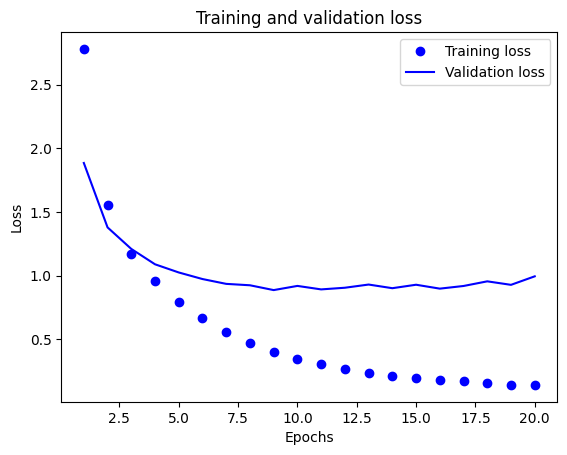
\includegraphics{chapters/01_jumpstart/jumpstart_files/figure-pdf/cell-19-output-1.png}

}

\end{figure}

If we wanted to make this graph more presentable we could do something
like:

\begin{Shaded}
\begin{Highlighting}[]
\NormalTok{ax }\OperatorTok{=}\NormalTok{ df\_spy.}\OperatorTok{\textbackslash{}}
\NormalTok{        plot(}
\NormalTok{            x }\OperatorTok{=} \StringTok{\textquotesingle{}date\textquotesingle{}}\NormalTok{,}
\NormalTok{            y }\OperatorTok{=} \StringTok{\textquotesingle{}adj\_close\textquotesingle{}}\NormalTok{,}
\NormalTok{            title }\OperatorTok{=} \StringTok{\textquotesingle{}SPY: 2014{-}2018\textquotesingle{}}\NormalTok{,}
\NormalTok{            grid }\OperatorTok{=} \VariableTok{True}\NormalTok{,}
\NormalTok{            style }\OperatorTok{=} \StringTok{\textquotesingle{}k\textquotesingle{}}\NormalTok{,}
\NormalTok{            alpha }\OperatorTok{=} \FloatTok{0.75}\NormalTok{,}
\NormalTok{            figsize }\OperatorTok{=}\NormalTok{ (}\DecValTok{9}\NormalTok{, }\DecValTok{4}\NormalTok{),}
\NormalTok{        )}\OperatorTok{;}
\NormalTok{ax.set\_xlabel(}\StringTok{\textquotesingle{}Trade Date\textquotesingle{}}\NormalTok{)}\OperatorTok{;}
\NormalTok{ax.set\_ylabel(}\StringTok{\textquotesingle{}Close Price\textquotesingle{}}\NormalTok{)}\OperatorTok{;}
\end{Highlighting}
\end{Shaded}

\begin{figure}[H]

{\centering 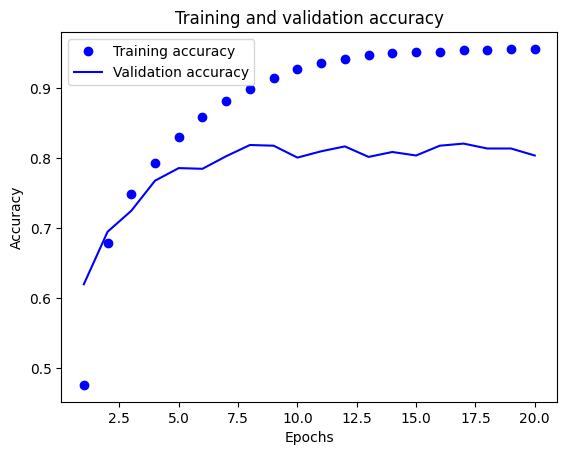
\includegraphics{chapters/01_jumpstart/jumpstart_files/figure-pdf/cell-20-output-1.png}

}

\end{figure}

Notice that the \texttt{ax} variable created above is a
\texttt{matplotlib} object.

\begin{Shaded}
\begin{Highlighting}[]
\BuiltInTok{type}\NormalTok{(ax)}
\end{Highlighting}
\end{Shaded}

\begin{verbatim}
matplotlib.axes._axes.Axes
\end{verbatim}

\hypertarget{visualizing-returns}{%
\section{Visualizing Returns}\label{visualizing-returns}}

\textbf{pandas} also gives us the ability to simultaneously plot two
different columns of a \texttt{DataFrame} in separate subplots of a
single graph. Here is what that code looks like:

\begin{Shaded}
\begin{Highlighting}[]
\NormalTok{df\_spy.plot(x}\OperatorTok{=}\StringTok{\textquotesingle{}date\textquotesingle{}}\NormalTok{, y}\OperatorTok{=}\NormalTok{[}\StringTok{\textquotesingle{}adj\_close\textquotesingle{}}\NormalTok{, }\StringTok{\textquotesingle{}ret\textquotesingle{}}\NormalTok{,], subplots}\OperatorTok{=}\VariableTok{True}\NormalTok{, style}\OperatorTok{=}\StringTok{\textquotesingle{}k\textquotesingle{}}\NormalTok{, alpha}\OperatorTok{=}\FloatTok{0.75}\NormalTok{, figsize}\OperatorTok{=}\NormalTok{(}\DecValTok{9}\NormalTok{, }\DecValTok{8}\NormalTok{), grid}\OperatorTok{=}\VariableTok{True}\NormalTok{)}\OperatorTok{;}
\end{Highlighting}
\end{Shaded}

\begin{figure}[H]

{\centering 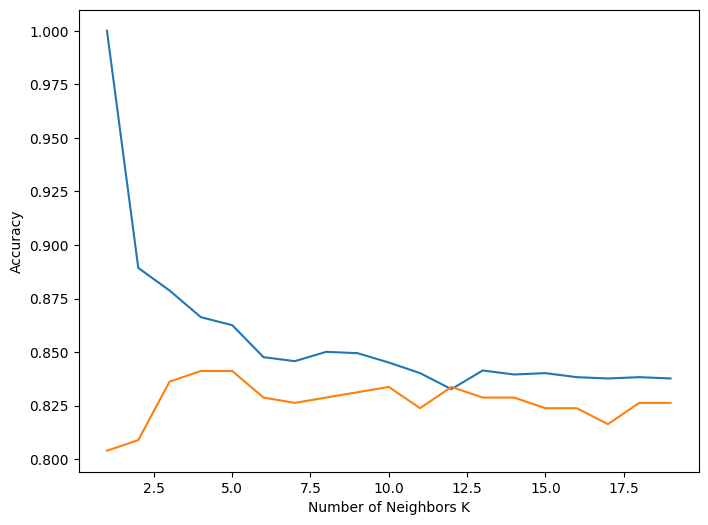
\includegraphics{chapters/01_jumpstart/jumpstart_files/figure-pdf/cell-22-output-1.png}

}

\end{figure}

The \texttt{returns} graph above is a bit of a hack, it doesn't really
make sense to create a line graph of consecutive returns. However,
because there are so many days jammed into the x-axis, it creates a
desirable effect and it used all the time in finance to demonstrate
properties of volatility.

Notice that whenever there is a sharp drop in the \texttt{adj\_close}
price graph, that the magnitude of the nearby returns becomes large. In
contrast, during periods of steady growth (e.g.~all of 2017) the
magnitude of the returns is small. This is precisely the leverage
effect.

\hypertarget{calculating-realized-volatility}{%
\section{Calculating Realized
Volatility}\label{calculating-realized-volatility}}

Realized volatility is defined as the standard deviation of the daily
returns; it indicates how much variability in the stock price there has
been. It is a matter of convention to annualize this quantity, so we
multiply it by \(\sqrt{252}\).

The following vectorized code calculates a rolling 2-month volatility
for our SPY price data.

\begin{Shaded}
\begin{Highlighting}[]
\NormalTok{df\_spy[}\StringTok{\textquotesingle{}ret\textquotesingle{}}\NormalTok{].rolling(}\DecValTok{42}\NormalTok{).std() }\OperatorTok{*}\NormalTok{ np.sqrt(}\DecValTok{252}\NormalTok{)}
\end{Highlighting}
\end{Shaded}

\begin{verbatim}
0            NaN
1            NaN
2            NaN
3            NaN
4            NaN
          ...   
1253    0.226735
1254    0.252813
1255    0.249195
1256    0.246019
1257    0.247027
Name: ret, Length: 1258, dtype: float64
\end{verbatim}

Let's add these realized volatility calculations to\texttt{df\_spy} this
with the following code.

\begin{Shaded}
\begin{Highlighting}[]
\NormalTok{df\_spy[}\StringTok{\textquotesingle{}realized\_vol\textquotesingle{}}\NormalTok{] }\OperatorTok{=}\NormalTok{ df\_spy[}\StringTok{\textquotesingle{}ret\textquotesingle{}}\NormalTok{].rolling(}\DecValTok{42}\NormalTok{).std() }\OperatorTok{*}\NormalTok{ np.sqrt(}\DecValTok{252}\NormalTok{)}
\NormalTok{df\_spy}
\end{Highlighting}
\end{Shaded}

\begin{longtable}[]{@{}lllll@{}}
\toprule\noalign{}
& date & adj\_close & ret & realized\_vol \\
\midrule\noalign{}
\endhead
\bottomrule\noalign{}
\endlastfoot
0 & 2014-01-02 & 153.83 & NaN & NaN \\
1 & 2014-01-03 & 153.80 & -0.000195 & NaN \\
2 & 2014-01-06 & 153.36 & -0.002861 & NaN \\
3 & 2014-01-07 & 154.30 & 0.006129 & NaN \\
4 & 2014-01-08 & 154.33 & 0.000194 & NaN \\
... & ... & ... & ... & ... \\
1253 & 2018-12-24 & 217.60 & -0.026442 & 0.226735 \\
1254 & 2018-12-26 & 228.59 & 0.050506 & 0.252813 \\
1255 & 2018-12-27 & 230.35 & 0.007699 & 0.249195 \\
1256 & 2018-12-28 & 230.05 & -0.001302 & 0.246019 \\
1257 & 2018-12-31 & 232.07 & 0.008781 & 0.247027 \\
\end{longtable}

\hypertarget{visualizing-realized-volatility}{%
\section{Visualizing Realized
Volatility}\label{visualizing-realized-volatility}}

We can easily add \texttt{realized\_vol} to our graph with the following
code.

\begin{Shaded}
\begin{Highlighting}[]
\NormalTok{df\_spy.plot(x }\OperatorTok{=} \StringTok{\textquotesingle{}date\textquotesingle{}}\NormalTok{, }
\NormalTok{            y }\OperatorTok{=}\NormalTok{ [}\StringTok{\textquotesingle{}adj\_close\textquotesingle{}}\NormalTok{,}\StringTok{\textquotesingle{}ret\textquotesingle{}}\NormalTok{,}\StringTok{\textquotesingle{}realized\_vol\textquotesingle{}}\NormalTok{,], }
\NormalTok{            subplots}\OperatorTok{=}\VariableTok{True}\NormalTok{, style}\OperatorTok{=}\StringTok{\textquotesingle{}k\textquotesingle{}}\NormalTok{, alpha}\OperatorTok{=}\FloatTok{0.75}\NormalTok{, }
\NormalTok{            figsize}\OperatorTok{=}\NormalTok{(}\DecValTok{9}\NormalTok{, }\DecValTok{12}\NormalTok{), }
\NormalTok{            grid}\OperatorTok{=}\VariableTok{True}\NormalTok{)}\OperatorTok{;}
\end{Highlighting}
\end{Shaded}

\begin{figure}[H]

{\centering 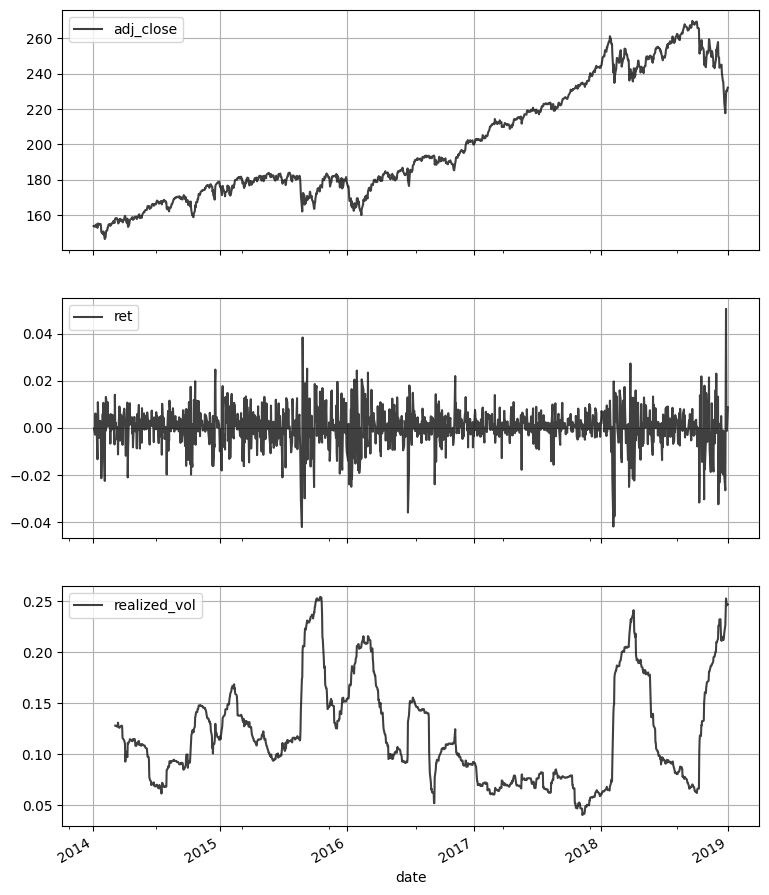
\includegraphics{chapters/01_jumpstart/jumpstart_files/figure-pdf/cell-25-output-1.png}

}

\end{figure}

This graph is an excellent illustration of the leverage effect. When SPY
suffers losses, there is a spike in realized volatility, which is to say
that the magnitude of the nearby returns increases.

\hypertarget{further-reading}{%
\section{Further Reading}\label{further-reading}}

\emph{Python Data Science Handbook} - Jake VanderPlas

\emph{Python for Finance 2e} - Yves Hilpisch

\emph{Python for Data Analysis 3e} - Wes McKinney

\part{Basic Data Wrangling}

\hypertarget{dataframe-basics}{%
\chapter{\texorpdfstring{\texttt{DataFrame}
Basics}{DataFrame Basics}}\label{dataframe-basics}}

In this chapter we cover the basics of working with \texttt{DataFrames}
in \textbf{pandas}.

\hypertarget{importing-packages-1}{%
\section{Importing Packages}\label{importing-packages-1}}

Let's begin by importing the packages that we will need.

\begin{Shaded}
\begin{Highlighting}[]
\ImportTok{import}\NormalTok{ pandas }\ImportTok{as}\NormalTok{ pd}
\ImportTok{import}\NormalTok{ yfinance }\ImportTok{as}\NormalTok{ yf}
\NormalTok{yf.pdr\_override()}
\ImportTok{from}\NormalTok{ pandas\_datareader }\ImportTok{import}\NormalTok{ data }\ImportTok{as}\NormalTok{ pdr}
\NormalTok{pd.set\_option(}\StringTok{\textquotesingle{}display.max\_rows\textquotesingle{}}\NormalTok{, }\DecValTok{10}\NormalTok{)}
\end{Highlighting}
\end{Shaded}

\hypertarget{reading-in-data}{%
\section{Reading-In Data}\label{reading-in-data}}

Next, let's use \textbf{pandas\_datareader} to read-in SPY prices from
March 2020. SPY is an ETF that tracks the S\&P500 index.

\begin{Shaded}
\begin{Highlighting}[]
\NormalTok{df\_spy }\OperatorTok{=}\NormalTok{ pdr.get\_data\_yahoo(}\StringTok{\textquotesingle{}SPY\textquotesingle{}}\NormalTok{, start}\OperatorTok{=}\StringTok{\textquotesingle{}2020{-}02{-}28\textquotesingle{}}\NormalTok{, end}\OperatorTok{=}\StringTok{\textquotesingle{}2020{-}03{-}31\textquotesingle{}}\NormalTok{)}
\NormalTok{df\_spy }\OperatorTok{=}\NormalTok{ df\_spy.}\BuiltInTok{round}\NormalTok{(}\DecValTok{2}\NormalTok{)}
\NormalTok{df\_spy.head()}
\end{Highlighting}
\end{Shaded}

\begin{verbatim}
[*********************100%***********************]  1 of 1 completed
\end{verbatim}

\begin{longtable}[]{@{}lllllll@{}}
\toprule\noalign{}
& Open & High & Low & Close & Adj Close & Volume \\
Date & & & & & & \\
\midrule\noalign{}
\endhead
\bottomrule\noalign{}
\endlastfoot
2020-02-28 & 288.70 & 297.89 & 285.54 & 296.26 & 280.31 & 384975800 \\
2020-03-02 & 298.21 & 309.16 & 294.46 & 309.09 & 292.45 & 238703600 \\
2020-03-03 & 309.50 & 313.84 & 297.57 & 300.24 & 284.07 & 300139100 \\
2020-03-04 & 306.12 & 313.10 & 303.33 & 312.86 & 296.01 & 176613400 \\
2020-03-05 & 304.98 & 308.47 & 300.01 & 302.46 & 286.17 & 186366800 \\
\end{longtable}

Let's also make the \texttt{Date} a regular column, instead of an index,
and also make the column names snake-case.

\begin{Shaded}
\begin{Highlighting}[]
\NormalTok{df\_spy.reset\_index(drop}\OperatorTok{=}\VariableTok{False}\NormalTok{, inplace}\OperatorTok{=}\VariableTok{True}\NormalTok{)}
\NormalTok{df\_spy.columns }\OperatorTok{=}\NormalTok{ df\_spy.columns.}\BuiltInTok{str}\NormalTok{.lower().}\BuiltInTok{str}\NormalTok{.replace(}\StringTok{\textquotesingle{} \textquotesingle{}}\NormalTok{, }\StringTok{\textquotesingle{}\_\textquotesingle{}}\NormalTok{)}
\NormalTok{df\_spy.head()}
\end{Highlighting}
\end{Shaded}

\begin{longtable}[]{@{}llllllll@{}}
\toprule\noalign{}
& date & open & high & low & close & adj\_close & volume \\
\midrule\noalign{}
\endhead
\bottomrule\noalign{}
\endlastfoot
0 & 2020-02-28 & 288.70 & 297.89 & 285.54 & 296.26 & 280.31 &
384975800 \\
1 & 2020-03-02 & 298.21 & 309.16 & 294.46 & 309.09 & 292.45 &
238703600 \\
2 & 2020-03-03 & 309.50 & 313.84 & 297.57 & 300.24 & 284.07 &
300139100 \\
3 & 2020-03-04 & 306.12 & 313.10 & 303.33 & 312.86 & 296.01 &
176613400 \\
4 & 2020-03-05 & 304.98 & 308.47 & 300.01 & 302.46 & 286.17 &
186366800 \\
\end{longtable}

\hypertarget{exploring-a-dataframe}{%
\section{\texorpdfstring{Exploring a
\texttt{DataFrame}}{Exploring a DataFrame}}\label{exploring-a-dataframe}}

We can explore our \texttt{df\_spy} \texttt{DataFrame} in a variety of
ways.

First, we can first use the \texttt{type()} method to make sure what we
have created is in fact a \texttt{DataFrame}.

\begin{Shaded}
\begin{Highlighting}[]
\BuiltInTok{type}\NormalTok{(df\_spy)}
\end{Highlighting}
\end{Shaded}

\begin{verbatim}
pandas.core.frame.DataFrame
\end{verbatim}

Next, we can use the \texttt{.dtypes} attribute of the
\texttt{DataFrame} to see the data types of each of the columns.

\begin{Shaded}
\begin{Highlighting}[]
\NormalTok{df\_spy.dtypes}
\end{Highlighting}
\end{Shaded}

\begin{verbatim}
date         datetime64[ns]
open                float64
high                float64
low                 float64
close               float64
adj_close           float64
volume                int64
dtype: object
\end{verbatim}

We can also check the number of rows and columns by using the
\texttt{.shape} attribute.

\begin{Shaded}
\begin{Highlighting}[]
\NormalTok{df\_spy.shape}
\end{Highlighting}
\end{Shaded}

\begin{verbatim}
(22, 7)
\end{verbatim}

As we can see, our \texttt{DataFrame} \texttt{df\_spy} consists of 22
rows and 7 columns.

\begin{center}\rule{0.5\linewidth}{0.5pt}\end{center}

\textbf{Code Challenge:} Try the \texttt{DataFrame.info()} and
\texttt{DataFrame.describe()} methods on \texttt{df\_spy}.

\begin{Shaded}
\begin{Highlighting}[]
\NormalTok{df\_spy.info()}
\end{Highlighting}
\end{Shaded}

\begin{verbatim}
<class 'pandas.core.frame.DataFrame'>
RangeIndex: 22 entries, 0 to 21
Data columns (total 7 columns):
 #   Column     Non-Null Count  Dtype         
---  ------     --------------  -----         
 0   date       22 non-null     datetime64[ns]
 1   open       22 non-null     float64       
 2   high       22 non-null     float64       
 3   low        22 non-null     float64       
 4   close      22 non-null     float64       
 5   adj_close  22 non-null     float64       
 6   volume     22 non-null     int64         
dtypes: datetime64[ns](1), float64(5), int64(1)
memory usage: 1.3 KB
\end{verbatim}

\begin{Shaded}
\begin{Highlighting}[]
\NormalTok{df\_spy.describe().}\BuiltInTok{round}\NormalTok{(}\DecValTok{2}\NormalTok{)}
\end{Highlighting}
\end{Shaded}

\begin{longtable}[]{@{}llllllll@{}}
\toprule\noalign{}
& date & open & high & low & close & adj\_close & volume \\
\midrule\noalign{}
\endhead
\bottomrule\noalign{}
\endlastfoot
count & 22 & 22.00 & 22.00 & 22.00 & 22.00 & 22.00 & 2.200000e+01 \\
mean & 2020-03-14 12:00:00 & 265.03 & 272.89 & 258.81 & 266.54 & 252.62
& 2.780051e+08 \\
min & 2020-02-28 00:00:00 & 228.19 & 229.68 & 218.26 & 222.95 & 212.18 &
1.713695e+08 \\
25\% & 2020-03-06 18:00:00 & 243.12 & 256.22 & 237.14 & 244.06 & 232.24
& 2.362968e+08 \\
50\% & 2020-03-14 12:00:00 & 255.85 & 264.73 & 250.05 & 261.42 & 248.80
& 2.828830e+08 \\
75\% & 2020-03-22 06:00:00 & 287.68 & 295.55 & 282.53 & 294.30 & 278.46
& 3.218732e+08 \\
max & 2020-03-30 00:00:00 & 309.50 & 313.84 & 303.33 & 312.86 & 296.01 &
3.922207e+08 \\
std & NaN & 26.43 & 25.44 & 26.98 & 27.55 & 25.74 & 6.134551e+07 \\
\end{longtable}

\hypertarget{dataframe-columns}{%
\section{\texorpdfstring{\texttt{DataFrame}
Columns}{DataFrame Columns}}\label{dataframe-columns}}

In order to isolate a particular column of a \texttt{DataFrame} we can
use square brackets (\texttt{{[}\ {]}}). The following code isolates the
\texttt{close} price column of \texttt{df\_spy}.

\begin{Shaded}
\begin{Highlighting}[]
\NormalTok{df\_spy[}\StringTok{\textquotesingle{}close\textquotesingle{}}\NormalTok{]}
\end{Highlighting}
\end{Shaded}

\begin{verbatim}
0     296.26
1     309.09
2     300.24
3     312.86
4     302.46
       ...  
17    243.15
18    246.79
19    261.20
20    253.42
21    261.65
Name: close, Length: 22, dtype: float64
\end{verbatim}

\begin{center}\rule{0.5\linewidth}{0.5pt}\end{center}

\textbf{Code Challenge:} Isolate the \texttt{date} column of
\texttt{df\_spy}.

\begin{Shaded}
\begin{Highlighting}[]
\NormalTok{df\_spy[}\StringTok{\textquotesingle{}date\textquotesingle{}}\NormalTok{]}
\end{Highlighting}
\end{Shaded}

\begin{verbatim}
0    2020-02-28
1    2020-03-02
2    2020-03-03
3    2020-03-04
4    2020-03-05
        ...    
17   2020-03-24
18   2020-03-25
19   2020-03-26
20   2020-03-27
21   2020-03-30
Name: date, Length: 22, dtype: datetime64[ns]
\end{verbatim}

\begin{center}\rule{0.5\linewidth}{0.5pt}\end{center}

As we can see from the following code, each column of a
\texttt{DataFrame} is actually a different kind of \textbf{pandas}
structure called a \texttt{Series}.

\begin{Shaded}
\begin{Highlighting}[]
\BuiltInTok{type}\NormalTok{(df\_spy[}\StringTok{\textquotesingle{}close\textquotesingle{}}\NormalTok{])}
\end{Highlighting}
\end{Shaded}

\begin{verbatim}
pandas.core.series.Series
\end{verbatim}

Here is a bit of \textbf{pandas} inside baseball:

\begin{itemize}
\item
  A \texttt{DataFrame} is collection of columns that are glued together.
\item
  Each column is a \texttt{Series}.
\item
  A \texttt{Series} has two main attributes: 1) \texttt{.values}; 2)
  \texttt{.index}.
\item
  The \texttt{.values} component of a \texttt{Series} is a
  \texttt{numpy.array}.
\end{itemize}

Let's look at the \texttt{.values} attribute of the \texttt{close}
column of \texttt{df\_spy}.

\begin{Shaded}
\begin{Highlighting}[]
\NormalTok{df\_spy[}\StringTok{\textquotesingle{}close\textquotesingle{}}\NormalTok{].values}
\end{Highlighting}
\end{Shaded}

\begin{verbatim}
array([296.26, 309.09, 300.24, 312.86, 302.46, 297.46, 274.23, 288.42,
       274.36, 248.11, 269.32, 239.85, 252.8 , 240.  , 240.51, 228.8 ,
       222.95, 243.15, 246.79, 261.2 , 253.42, 261.65])
\end{verbatim}

\begin{center}\rule{0.5\linewidth}{0.5pt}\end{center}

\textbf{Code Challenge:} Verify that the \texttt{values} component of
the \texttt{close} column of \texttt{df\_spy} is in fact a a
\texttt{numpy.array}.

\begin{Shaded}
\begin{Highlighting}[]
\BuiltInTok{type}\NormalTok{(df\_spy[}\StringTok{\textquotesingle{}close\textquotesingle{}}\NormalTok{].values)}
\end{Highlighting}
\end{Shaded}

\begin{verbatim}
numpy.ndarray
\end{verbatim}

\begin{center}\rule{0.5\linewidth}{0.5pt}\end{center}

\hypertarget{component-wise-column-operations}{%
\section{Component-wise Column
Operations}\label{component-wise-column-operations}}

We can perform component-wise (i.e.~vector-like) calculations with
\texttt{DataFrame} columns.

The following code divides all the \texttt{close} prices by 100.

\begin{Shaded}
\begin{Highlighting}[]
\NormalTok{df\_spy[}\StringTok{\textquotesingle{}close\textquotesingle{}}\NormalTok{] }\OperatorTok{/} \DecValTok{100}
\end{Highlighting}
\end{Shaded}

\begin{verbatim}
0     2.9626
1     3.0909
2     3.0024
3     3.1286
4     3.0246
       ...  
17    2.4315
18    2.4679
19    2.6120
20    2.5342
21    2.6165
Name: close, Length: 22, dtype: float64
\end{verbatim}

We can also perform component-wise calculations between two colums.

Let's say we want to calculate the \emph{intraday range} of SPY for each
of the trade-dates in \texttt{df\_spy}; this is the difference between
the \texttt{high} and the \texttt{low} of each day. We can do this
easily from the columns of our \texttt{DataFrame}.

\begin{Shaded}
\begin{Highlighting}[]
\NormalTok{df\_spy[}\StringTok{\textquotesingle{}high\textquotesingle{}}\NormalTok{] }\OperatorTok{{-}}\NormalTok{ df\_spy[}\StringTok{\textquotesingle{}low\textquotesingle{}}\NormalTok{]}
\end{Highlighting}
\end{Shaded}

\begin{verbatim}
0     12.35
1     14.70
2     16.27
3      9.77
4      8.46
      ...  
17    10.30
18    16.60
19    13.75
20     9.76
21     8.90
Length: 22, dtype: float64
\end{verbatim}

\begin{center}\rule{0.5\linewidth}{0.5pt}\end{center}

\textbf{Code Challenge:} Calculate the difference between the
\texttt{close} and \texttt{open} columns of \texttt{df\_spy}.

\begin{Shaded}
\begin{Highlighting}[]
\NormalTok{df\_spy[}\StringTok{\textquotesingle{}close\textquotesingle{}}\NormalTok{] }\OperatorTok{{-}}\NormalTok{ df\_spy[}\StringTok{\textquotesingle{}open\textquotesingle{}}\NormalTok{]}
\end{Highlighting}
\end{Shaded}

\begin{verbatim}
0      7.56
1     10.88
2     -9.26
3      6.74
4     -2.52
      ...  
17     8.73
18     1.92
19    11.68
20     0.15
21     5.95
Length: 22, dtype: float64
\end{verbatim}

\begin{center}\rule{0.5\linewidth}{0.5pt}\end{center}

\hypertarget{adding-columns-via-variable-assignment}{%
\section{Adding Columns via Variable
Assignment}\label{adding-columns-via-variable-assignment}}

Let's say we want to save our intraday ranges back into \texttt{df\_spy}
for further analysis later. The most straightforward way to do this is
using variable assignment as follows.

\begin{Shaded}
\begin{Highlighting}[]
\NormalTok{df\_spy[}\StringTok{\textquotesingle{}intraday\_range\textquotesingle{}}\NormalTok{] }\OperatorTok{=}\NormalTok{ df\_spy[}\StringTok{\textquotesingle{}high\textquotesingle{}}\NormalTok{] }\OperatorTok{{-}}\NormalTok{ df\_spy[}\StringTok{\textquotesingle{}low\textquotesingle{}}\NormalTok{]}
\NormalTok{df\_spy.head()}
\end{Highlighting}
\end{Shaded}

\begin{longtable}[]{@{}lllllllll@{}}
\toprule\noalign{}
& date & open & high & low & close & adj\_close & volume &
intraday\_range \\
\midrule\noalign{}
\endhead
\bottomrule\noalign{}
\endlastfoot
0 & 2020-02-28 & 288.70 & 297.89 & 285.54 & 296.26 & 280.31 & 384975800
& 12.35 \\
1 & 2020-03-02 & 298.21 & 309.16 & 294.46 & 309.09 & 292.45 & 238703600
& 14.70 \\
2 & 2020-03-03 & 309.50 & 313.84 & 297.57 & 300.24 & 284.07 & 300139100
& 16.27 \\
3 & 2020-03-04 & 306.12 & 313.10 & 303.33 & 312.86 & 296.01 & 176613400
& 9.77 \\
4 & 2020-03-05 & 304.98 & 308.47 & 300.01 & 302.46 & 286.17 & 186366800
& 8.46 \\
\end{longtable}

\begin{center}\rule{0.5\linewidth}{0.5pt}\end{center}

\textbf{Code Challenge:} Add a new column to \texttt{df\_spy} called
\texttt{open\_to\_close} that consists of the difference between the
\texttt{close} and \texttt{open} of each day.

\begin{Shaded}
\begin{Highlighting}[]
\NormalTok{df\_spy[}\StringTok{\textquotesingle{}open\_to\_close\textquotesingle{}}\NormalTok{] }\OperatorTok{=}\NormalTok{ df\_spy[}\StringTok{\textquotesingle{}close\textquotesingle{}}\NormalTok{] }\OperatorTok{{-}}\NormalTok{ df\_spy[}\StringTok{\textquotesingle{}open\textquotesingle{}}\NormalTok{]}
\NormalTok{df\_spy.head()}
\end{Highlighting}
\end{Shaded}

\begin{longtable}[]{@{}llllllllll@{}}
\toprule\noalign{}
& date & open & high & low & close & adj\_close & volume &
intraday\_range & open\_to\_close \\
\midrule\noalign{}
\endhead
\bottomrule\noalign{}
\endlastfoot
0 & 2020-02-28 & 288.70 & 297.89 & 285.54 & 296.26 & 280.31 & 384975800
& 12.35 & 7.56 \\
1 & 2020-03-02 & 298.21 & 309.16 & 294.46 & 309.09 & 292.45 & 238703600
& 14.70 & 10.88 \\
2 & 2020-03-03 & 309.50 & 313.84 & 297.57 & 300.24 & 284.07 & 300139100
& 16.27 & -9.26 \\
3 & 2020-03-04 & 306.12 & 313.10 & 303.33 & 312.86 & 296.01 & 176613400
& 9.77 & 6.74 \\
4 & 2020-03-05 & 304.98 & 308.47 & 300.01 & 302.46 & 286.17 & 186366800
& 8.46 & -2.52 \\
\end{longtable}

\begin{center}\rule{0.5\linewidth}{0.5pt}\end{center}

\hypertarget{adding-columns-via-.assign}{%
\section{\texorpdfstring{Adding Columns via
\texttt{.assign()}}{Adding Columns via .assign()}}\label{adding-columns-via-.assign}}

A powerful but less intuitive way of adding a column to a
\texttt{DataFrame} uses the \texttt{.assign()} function, which makes use
of \texttt{lambda} functions (i.e.~anonymous functions).

The following code adds another column called
\texttt{intraday\_range\_assign}.

\begin{Shaded}
\begin{Highlighting}[]
\NormalTok{df\_spy.assign(intraday\_range\_assign }\OperatorTok{=} \KeywordTok{lambda}\NormalTok{ df: df[}\StringTok{\textquotesingle{}high\textquotesingle{}}\NormalTok{] }\OperatorTok{{-}}\NormalTok{ df[}\StringTok{\textquotesingle{}low\textquotesingle{}}\NormalTok{])}
\end{Highlighting}
\end{Shaded}

\begin{longtable}[]{@{}lllllllllll@{}}
\toprule\noalign{}
& date & open & high & low & close & adj\_close & volume &
intraday\_range & open\_to\_close & intraday\_range\_assign \\
\midrule\noalign{}
\endhead
\bottomrule\noalign{}
\endlastfoot
0 & 2020-02-28 & 288.70 & 297.89 & 285.54 & 296.26 & 280.31 & 384975800
& 12.35 & 7.56 & 12.35 \\
1 & 2020-03-02 & 298.21 & 309.16 & 294.46 & 309.09 & 292.45 & 238703600
& 14.70 & 10.88 & 14.70 \\
2 & 2020-03-03 & 309.50 & 313.84 & 297.57 & 300.24 & 284.07 & 300139100
& 16.27 & -9.26 & 16.27 \\
3 & 2020-03-04 & 306.12 & 313.10 & 303.33 & 312.86 & 296.01 & 176613400
& 9.77 & 6.74 & 9.77 \\
4 & 2020-03-05 & 304.98 & 308.47 & 300.01 & 302.46 & 286.17 & 186366800
& 8.46 & -2.52 & 8.46 \\
... & ... & ... & ... & ... & ... & ... & ... & ... & ... & ... \\
17 & 2020-03-24 & 234.42 & 244.10 & 233.80 & 243.15 & 231.41 & 235494500
& 10.30 & 8.73 & 10.30 \\
18 & 2020-03-25 & 244.87 & 256.35 & 239.75 & 246.79 & 234.87 & 299430300
& 16.60 & 1.92 & 16.60 \\
19 & 2020-03-26 & 249.52 & 262.80 & 249.05 & 261.20 & 248.59 & 257632800
& 13.75 & 11.68 & 13.75 \\
20 & 2020-03-27 & 253.27 & 260.81 & 251.05 & 253.42 & 241.18 & 224341200
& 9.76 & 0.15 & 9.76 \\
21 & 2020-03-30 & 255.70 & 262.43 & 253.53 & 261.65 & 249.02 & 171369500
& 8.90 & 5.95 & 8.90 \\
\end{longtable}

\begin{center}\rule{0.5\linewidth}{0.5pt}\end{center}

\textbf{Code Challenge:} Verify that the column
\texttt{intraday\_range\_assign} was not actually added to the
\texttt{df\_spy}.

\begin{Shaded}
\begin{Highlighting}[]
\NormalTok{df\_spy.head()}
\end{Highlighting}
\end{Shaded}

\begin{longtable}[]{@{}llllllllll@{}}
\toprule\noalign{}
& date & open & high & low & close & adj\_close & volume &
intraday\_range & open\_to\_close \\
\midrule\noalign{}
\endhead
\bottomrule\noalign{}
\endlastfoot
0 & 2020-02-28 & 288.70 & 297.89 & 285.54 & 296.26 & 280.31 & 384975800
& 12.35 & 7.56 \\
1 & 2020-03-02 & 298.21 & 309.16 & 294.46 & 309.09 & 292.45 & 238703600
& 14.70 & 10.88 \\
2 & 2020-03-03 & 309.50 & 313.84 & 297.57 & 300.24 & 284.07 & 300139100
& 16.27 & -9.26 \\
3 & 2020-03-04 & 306.12 & 313.10 & 303.33 & 312.86 & 296.01 & 176613400
& 9.77 & 6.74 \\
4 & 2020-03-05 & 304.98 & 308.47 & 300.01 & 302.46 & 286.17 & 186366800
& 8.46 & -2.52 \\
\end{longtable}

\begin{center}\rule{0.5\linewidth}{0.5pt}\end{center}

In order to add the \texttt{intraday\_range\_assign} column to
\texttt{df\_spy} we will need to reassign to it.

\begin{Shaded}
\begin{Highlighting}[]
\NormalTok{df\_spy }\OperatorTok{=}\NormalTok{ df\_spy.assign(intraday\_range\_assign }\OperatorTok{=} \KeywordTok{lambda}\NormalTok{ df: df[}\StringTok{\textquotesingle{}high\textquotesingle{}}\NormalTok{] }\OperatorTok{{-}}\NormalTok{ df[}\StringTok{\textquotesingle{}low\textquotesingle{}}\NormalTok{])}
\NormalTok{df\_spy.head()}
\end{Highlighting}
\end{Shaded}

\begin{longtable}[]{@{}lllllllllll@{}}
\toprule\noalign{}
& date & open & high & low & close & adj\_close & volume &
intraday\_range & open\_to\_close & intraday\_range\_assign \\
\midrule\noalign{}
\endhead
\bottomrule\noalign{}
\endlastfoot
0 & 2020-02-28 & 288.70 & 297.89 & 285.54 & 296.26 & 280.31 & 384975800
& 12.35 & 7.56 & 12.35 \\
1 & 2020-03-02 & 298.21 & 309.16 & 294.46 & 309.09 & 292.45 & 238703600
& 14.70 & 10.88 & 14.70 \\
2 & 2020-03-03 & 309.50 & 313.84 & 297.57 & 300.24 & 284.07 & 300139100
& 16.27 & -9.26 & 16.27 \\
3 & 2020-03-04 & 306.12 & 313.10 & 303.33 & 312.86 & 296.01 & 176613400
& 9.77 & 6.74 & 9.77 \\
4 & 2020-03-05 & 304.98 & 308.47 & 300.01 & 302.46 & 286.17 & 186366800
& 8.46 & -2.52 & 8.46 \\
\end{longtable}

\begin{center}\rule{0.5\linewidth}{0.5pt}\end{center}

\textbf{Code Challenge:} Use \texttt{.assign()} to create a new column
in \texttt{df\_spy}, call it \texttt{open\_to\_close\_assign}, that
contains the difference between the \texttt{close} and \texttt{open}.

\begin{Shaded}
\begin{Highlighting}[]
\NormalTok{df\_spy }\OperatorTok{=}\NormalTok{ df\_spy.assign(open\_to\_close\_assign }\OperatorTok{=} \KeywordTok{lambda}\NormalTok{ df: df[}\StringTok{\textquotesingle{}close\textquotesingle{}}\NormalTok{] }\OperatorTok{{-}}\NormalTok{ df[}\StringTok{\textquotesingle{}open\textquotesingle{}}\NormalTok{])}
\NormalTok{df\_spy.head()}
\end{Highlighting}
\end{Shaded}

\begin{longtable}[]{@{}llllllllllll@{}}
\toprule\noalign{}
& date & open & high & low & close & adj\_close & volume &
intraday\_range & open\_to\_close & intraday\_range\_assign &
open\_to\_close\_assign \\
\midrule\noalign{}
\endhead
\bottomrule\noalign{}
\endlastfoot
0 & 2020-02-28 & 288.70 & 297.89 & 285.54 & 296.26 & 280.31 & 384975800
& 12.35 & 7.56 & 12.35 & 7.56 \\
1 & 2020-03-02 & 298.21 & 309.16 & 294.46 & 309.09 & 292.45 & 238703600
& 14.70 & 10.88 & 14.70 & 10.88 \\
2 & 2020-03-03 & 309.50 & 313.84 & 297.57 & 300.24 & 284.07 & 300139100
& 16.27 & -9.26 & 16.27 & -9.26 \\
3 & 2020-03-04 & 306.12 & 313.10 & 303.33 & 312.86 & 296.01 & 176613400
& 9.77 & 6.74 & 9.77 & 6.74 \\
4 & 2020-03-05 & 304.98 & 308.47 & 300.01 & 302.46 & 286.17 & 186366800
& 8.46 & -2.52 & 8.46 & -2.52 \\
\end{longtable}

\begin{center}\rule{0.5\linewidth}{0.5pt}\end{center}

\hypertarget{method-chaining}{%
\section{Method Chaining}\label{method-chaining}}

The value of \texttt{.assign()} becomes clear when we start
\emph{chaining} methods together.

In order to see this let's first \texttt{drop} the columns that we
created.

\begin{Shaded}
\begin{Highlighting}[]
\NormalTok{lst\_cols }\OperatorTok{=}\NormalTok{ [}\StringTok{\textquotesingle{}intraday\_range\textquotesingle{}}\NormalTok{, }\StringTok{\textquotesingle{}open\_to\_close\textquotesingle{}}\NormalTok{, }\StringTok{\textquotesingle{}intraday\_range\_assign\textquotesingle{}}\NormalTok{, }\StringTok{\textquotesingle{}open\_to\_close\_assign\textquotesingle{}}\NormalTok{]}
\NormalTok{df\_spy.drop(columns}\OperatorTok{=}\NormalTok{lst\_cols, inplace}\OperatorTok{=}\VariableTok{True}\NormalTok{)}
\NormalTok{df\_spy.head()}
\end{Highlighting}
\end{Shaded}

\begin{longtable}[]{@{}llllllll@{}}
\toprule\noalign{}
& date & open & high & low & close & adj\_close & volume \\
\midrule\noalign{}
\endhead
\bottomrule\noalign{}
\endlastfoot
0 & 2020-02-28 & 288.70 & 297.89 & 285.54 & 296.26 & 280.31 &
384975800 \\
1 & 2020-03-02 & 298.21 & 309.16 & 294.46 & 309.09 & 292.45 &
238703600 \\
2 & 2020-03-03 & 309.50 & 313.84 & 297.57 & 300.24 & 284.07 &
300139100 \\
3 & 2020-03-04 & 306.12 & 313.10 & 303.33 & 312.86 & 296.01 &
176613400 \\
4 & 2020-03-05 & 304.98 & 308.47 & 300.01 & 302.46 & 286.17 &
186366800 \\
\end{longtable}

The following code adds the \texttt{intraday} and and
\texttt{open\_to\_close} columns at the same time.

\begin{Shaded}
\begin{Highlighting}[]
\NormalTok{df\_spy }\OperatorTok{=} \OperatorTok{\textbackslash{}}
\NormalTok{    (}
\NormalTok{    df\_spy}
\NormalTok{        .assign(intraday\_range }\OperatorTok{=} \KeywordTok{lambda}\NormalTok{ df: df[}\StringTok{\textquotesingle{}high\textquotesingle{}}\NormalTok{] }\OperatorTok{{-}}\NormalTok{ df[}\StringTok{\textquotesingle{}low\textquotesingle{}}\NormalTok{])}
\NormalTok{        .assign(open\_to\_close }\OperatorTok{=} \KeywordTok{lambda}\NormalTok{ df: df[}\StringTok{\textquotesingle{}close\textquotesingle{}}\NormalTok{] }\OperatorTok{{-}}\NormalTok{ df[}\StringTok{\textquotesingle{}open\textquotesingle{}}\NormalTok{])}
\NormalTok{    )}
\NormalTok{df\_spy.head()}
\end{Highlighting}
\end{Shaded}

\begin{longtable}[]{@{}llllllllll@{}}
\toprule\noalign{}
& date & open & high & low & close & adj\_close & volume &
intraday\_range & open\_to\_close \\
\midrule\noalign{}
\endhead
\bottomrule\noalign{}
\endlastfoot
0 & 2020-02-28 & 288.70 & 297.89 & 285.54 & 296.26 & 280.31 & 384975800
& 12.35 & 7.56 \\
1 & 2020-03-02 & 298.21 & 309.16 & 294.46 & 309.09 & 292.45 & 238703600
& 14.70 & 10.88 \\
2 & 2020-03-03 & 309.50 & 313.84 & 297.57 & 300.24 & 284.07 & 300139100
& 16.27 & -9.26 \\
3 & 2020-03-04 & 306.12 & 313.10 & 303.33 & 312.86 & 296.01 & 176613400
& 9.77 & 6.74 \\
4 & 2020-03-05 & 304.98 & 308.47 & 300.01 & 302.46 & 286.17 & 186366800
& 8.46 & -2.52 \\
\end{longtable}

\begin{center}\rule{0.5\linewidth}{0.5pt}\end{center}

\textbf{Code Challenge:} Use \texttt{.assign()} to add a two new column
to \texttt{df\_spy}:

\begin{enumerate}
\def\labelenumi{\arabic{enumi}.}
\tightlist
\item
  the difference between the \texttt{close} and \texttt{adj\_close}
\item
  the average of the \texttt{low} and \texttt{open}
\end{enumerate}

\begin{Shaded}
\begin{Highlighting}[]
\NormalTok{df\_spy }\OperatorTok{=} \OperatorTok{\textbackslash{}}
\NormalTok{    (}
\NormalTok{    df\_spy}
\NormalTok{        .assign(div }\OperatorTok{=} \KeywordTok{lambda}\NormalTok{ df: df[}\StringTok{\textquotesingle{}close\textquotesingle{}}\NormalTok{] }\OperatorTok{{-}}\NormalTok{ df[}\StringTok{\textquotesingle{}adj\_close\textquotesingle{}}\NormalTok{])}
\NormalTok{        .assign(avg }\OperatorTok{=} \KeywordTok{lambda}\NormalTok{ df: (df[}\StringTok{\textquotesingle{}low\textquotesingle{}}\NormalTok{] }\OperatorTok{+}\NormalTok{ df[}\StringTok{\textquotesingle{}open\textquotesingle{}}\NormalTok{]) }\OperatorTok{/} \DecValTok{2}\NormalTok{)}
\NormalTok{    )}
\NormalTok{df\_spy.head()}
\end{Highlighting}
\end{Shaded}

\begin{longtable}[]{@{}llllllllllll@{}}
\toprule\noalign{}
& date & open & high & low & close & adj\_close & volume &
intraday\_range & open\_to\_close & div & avg \\
\midrule\noalign{}
\endhead
\bottomrule\noalign{}
\endlastfoot
0 & 2020-02-28 & 288.70 & 297.89 & 285.54 & 296.26 & 280.31 & 384975800
& 12.35 & 7.56 & 15.95 & 287.120 \\
1 & 2020-03-02 & 298.21 & 309.16 & 294.46 & 309.09 & 292.45 & 238703600
& 14.70 & 10.88 & 16.64 & 296.335 \\
2 & 2020-03-03 & 309.50 & 313.84 & 297.57 & 300.24 & 284.07 & 300139100
& 16.27 & -9.26 & 16.17 & 303.535 \\
3 & 2020-03-04 & 306.12 & 313.10 & 303.33 & 312.86 & 296.01 & 176613400
& 9.77 & 6.74 & 16.85 & 304.725 \\
4 & 2020-03-05 & 304.98 & 308.47 & 300.01 & 302.46 & 286.17 & 186366800
& 8.46 & -2.52 & 16.29 & 302.495 \\
\end{longtable}

\begin{center}\rule{0.5\linewidth}{0.5pt}\end{center}

\hypertarget{aggregating-calulations-on-series}{%
\section{\texorpdfstring{Aggregating Calulations on
\texttt{Series}}{Aggregating Calulations on Series}}\label{aggregating-calulations-on-series}}

\texttt{Series} have a variety of built-in aggregation functions.

For example, we can use the following code to calculate the total SPY
volume during March 2020.

\begin{Shaded}
\begin{Highlighting}[]
\NormalTok{df\_spy[}\StringTok{\textquotesingle{}volume\textquotesingle{}}\NormalTok{].}\BuiltInTok{sum}\NormalTok{()}
\end{Highlighting}
\end{Shaded}

\begin{verbatim}
6116112300
\end{verbatim}

Here are some summary statistics on the \texttt{intraday\_range} column
that we added to our \texttt{DataFrame} earlier.

\begin{Shaded}
\begin{Highlighting}[]
\BuiltInTok{print}\NormalTok{(}\StringTok{"Mean:  "}\NormalTok{, df\_spy[}\StringTok{\textquotesingle{}intraday\_range\textquotesingle{}}\NormalTok{].mean()) }\CommentTok{\# average}
\BuiltInTok{print}\NormalTok{(}\StringTok{"St Dev: "}\NormalTok{, df\_spy[}\StringTok{\textquotesingle{}intraday\_range\textquotesingle{}}\NormalTok{].std()) }\CommentTok{\# standard deviation}
\BuiltInTok{print}\NormalTok{(}\StringTok{"Min:    "}\NormalTok{ , df\_spy[}\StringTok{\textquotesingle{}intraday\_range\textquotesingle{}}\NormalTok{].}\BuiltInTok{min}\NormalTok{()) }\CommentTok{\# minimum}
\BuiltInTok{print}\NormalTok{(}\StringTok{"Max:   "}\NormalTok{ , df\_spy[}\StringTok{\textquotesingle{}intraday\_range\textquotesingle{}}\NormalTok{].}\BuiltInTok{max}\NormalTok{()) }\CommentTok{\# maximum}
\end{Highlighting}
\end{Shaded}

\begin{verbatim}
Mean:   14.077727272727275
St Dev:  4.28352428533215
Min:     8.460000000000036
Max:    22.960000000000008
\end{verbatim}

\begin{center}\rule{0.5\linewidth}{0.5pt}\end{center}

\textbf{Code Challenge:} Calculate the average daily \texttt{volume} for
the trade dates in \texttt{df\_spy}.

\begin{Shaded}
\begin{Highlighting}[]
\NormalTok{df\_spy[}\StringTok{\textquotesingle{}volume\textquotesingle{}}\NormalTok{].mean()}
\end{Highlighting}
\end{Shaded}

\begin{verbatim}
278005104.54545456
\end{verbatim}

\begin{center}\rule{0.5\linewidth}{0.5pt}\end{center}

\hypertarget{related-reading}{%
\section{Related Reading}\label{related-reading}}

\emph{Python Data Science Handbook} - Section 3.1 - Introducing Pandas
Objects

\emph{Python Data Science Handbook} - Section 2.1 - Understanding Data
Types in Python

\emph{Python Data Science Handbook} - Section 2.2 - The Basics of NumPy
Arrays

\emph{Python Data Science Handbook} - Section 2.3 - Computation on NumPy
Arrays: Universal Functions

\emph{Python Data Science Handbook} - Section 2.4 - Aggregations: Min,
Max, and Everything In Between

\hypertarget{dataframe-indexing-and-slicing}{%
\chapter{\texorpdfstring{\texttt{DataFrame} Indexing and
Slicing}{DataFrame Indexing and Slicing}}\label{dataframe-indexing-and-slicing}}

Accessing a specific row of a \texttt{DataFrame} by its location is
referred to as \emph{indexing}. Accessing a sequence of contiguous rows
is referred to as \emph{slicing}.

The purpose of this chapter is to survey various methods for indexing
and slicing in \textbf{pandas}.

\hypertarget{importing-packages-2}{%
\section{Importing Packages}\label{importing-packages-2}}

Let's begin by importing the packages that we will need.

\begin{Shaded}
\begin{Highlighting}[]
\ImportTok{import}\NormalTok{ pandas }\ImportTok{as}\NormalTok{ pd}
\ImportTok{import}\NormalTok{ yfinance }\ImportTok{as}\NormalTok{ yf}
\NormalTok{yf.pdr\_override()}
\ImportTok{from}\NormalTok{ pandas\_datareader }\ImportTok{import}\NormalTok{ data }\ImportTok{as}\NormalTok{ pdr}
\NormalTok{pd.set\_option(}\StringTok{\textquotesingle{}display.max\_rows\textquotesingle{}}\NormalTok{, }\DecValTok{10}\NormalTok{)}
\end{Highlighting}
\end{Shaded}

\hypertarget{reading-in-data-1}{%
\section{Reading-In Data}\label{reading-in-data-1}}

Next, lets grab some data from Yahoo finance. In particular, we'll grab
\texttt{SPY} price data from July 2021.

\begin{Shaded}
\begin{Highlighting}[]
\NormalTok{df\_spy }\OperatorTok{=}\NormalTok{ pdr.get\_data\_yahoo(}\StringTok{\textquotesingle{}SPY\textquotesingle{}}\NormalTok{, start}\OperatorTok{=}\StringTok{\textquotesingle{}2021{-}06{-}30\textquotesingle{}}\NormalTok{, end}\OperatorTok{=}\StringTok{\textquotesingle{}2021{-}07{-}31\textquotesingle{}}\NormalTok{)}
\NormalTok{df\_spy }\OperatorTok{=}\NormalTok{ df\_spy.}\BuiltInTok{round}\NormalTok{(}\DecValTok{2}\NormalTok{)}
\NormalTok{df\_spy.head()}
\end{Highlighting}
\end{Shaded}

\begin{verbatim}
[*********************100%***********************]  1 of 1 completed
\end{verbatim}

\begin{longtable}[]{@{}lllllll@{}}
\toprule\noalign{}
& Open & High & Low & Close & Adj Close & Volume \\
Date & & & & & & \\
\midrule\noalign{}
\endhead
\bottomrule\noalign{}
\endlastfoot
2021-06-30 & 427.21 & 428.78 & 427.18 & 428.06 & 415.28 & 64827900 \\
2021-07-01 & 428.87 & 430.60 & 428.80 & 430.43 & 417.58 & 53441000 \\
2021-07-02 & 431.67 & 434.10 & 430.52 & 433.72 & 420.77 & 57697700 \\
2021-07-06 & 433.78 & 434.01 & 430.01 & 432.93 & 420.00 & 68710400 \\
2021-07-07 & 433.66 & 434.76 & 431.51 & 434.46 & 421.49 & 63549500 \\
\end{longtable}

The following code resets the index so that \texttt{Date} is a regular
column; it also puts the column names into snake-case.

\begin{Shaded}
\begin{Highlighting}[]
\NormalTok{df\_spy.reset\_index(inplace}\OperatorTok{=}\VariableTok{True}\NormalTok{)}
\NormalTok{df\_spy.columns }\OperatorTok{=}\NormalTok{ df\_spy.columns.}\BuiltInTok{str}\NormalTok{.lower().}\BuiltInTok{str}\NormalTok{.replace(}\StringTok{\textquotesingle{} \textquotesingle{}}\NormalTok{, }\StringTok{\textquotesingle{}\_\textquotesingle{}}\NormalTok{)}
\NormalTok{df\_spy.head()}
\end{Highlighting}
\end{Shaded}

\begin{longtable}[]{@{}llllllll@{}}
\toprule\noalign{}
& date & open & high & low & close & adj\_close & volume \\
\midrule\noalign{}
\endhead
\bottomrule\noalign{}
\endlastfoot
0 & 2021-06-30 & 427.21 & 428.78 & 427.18 & 428.06 & 415.28 &
64827900 \\
1 & 2021-07-01 & 428.87 & 430.60 & 428.80 & 430.43 & 417.58 &
53441000 \\
2 & 2021-07-02 & 431.67 & 434.10 & 430.52 & 433.72 & 420.77 &
57697700 \\
3 & 2021-07-06 & 433.78 & 434.01 & 430.01 & 432.93 & 420.00 &
68710400 \\
4 & 2021-07-07 & 433.66 & 434.76 & 431.51 & 434.46 & 421.49 &
63549500 \\
\end{longtable}

It is often useful to look at the data type of each of the columns of a
new data set. We can do so with the \texttt{DataFrame.dtypes} attribute.

\begin{Shaded}
\begin{Highlighting}[]
\NormalTok{df\_spy.dtypes}
\end{Highlighting}
\end{Shaded}

\begin{verbatim}
date         datetime64[ns]
open                float64
high                float64
low                 float64
close               float64
adj_close           float64
volume                int64
dtype: object
\end{verbatim}

\hypertarget{row-slicing}{%
\section{Row Slicing}\label{row-slicing}}

The simplest way to slice a \texttt{DataFrame} is to use square
brackets: \texttt{{[}{]}}. The syntax \texttt{df{[}i:j{]}} will generate
a \texttt{DataFrame} who's first row is the \texttt{i}th row of
\texttt{df} and who's last row is the \texttt{(j-1)}th row of
\texttt{df}. Let's demonstrate this with a some examples:

Starting from the 0th row, and ending with the 0th row:

\begin{Shaded}
\begin{Highlighting}[]
\NormalTok{df\_spy[}\DecValTok{0}\NormalTok{:}\DecValTok{1}\NormalTok{]}
\end{Highlighting}
\end{Shaded}

\begin{longtable}[]{@{}llllllll@{}}
\toprule\noalign{}
& date & open & high & low & close & adj\_close & volume \\
\midrule\noalign{}
\endhead
\bottomrule\noalign{}
\endlastfoot
0 & 2021-06-30 & 427.21 & 428.78 & 427.18 & 428.06 & 415.28 &
64827900 \\
\end{longtable}

Starting with the 3rd row, and ending with the 6th row:

\begin{Shaded}
\begin{Highlighting}[]
\NormalTok{df\_spy[}\DecValTok{3}\NormalTok{:}\DecValTok{7}\NormalTok{]}
\end{Highlighting}
\end{Shaded}

\begin{longtable}[]{@{}llllllll@{}}
\toprule\noalign{}
& date & open & high & low & close & adj\_close & volume \\
\midrule\noalign{}
\endhead
\bottomrule\noalign{}
\endlastfoot
3 & 2021-07-06 & 433.78 & 434.01 & 430.01 & 432.93 & 420.00 &
68710400 \\
4 & 2021-07-07 & 433.66 & 434.76 & 431.51 & 434.46 & 421.49 &
63549500 \\
5 & 2021-07-08 & 428.78 & 431.73 & 427.52 & 430.92 & 418.05 &
97595200 \\
6 & 2021-07-09 & 432.53 & 435.84 & 430.71 & 435.52 & 422.51 &
76238600 \\
\end{longtable}

\begin{center}\rule{0.5\linewidth}{0.5pt}\end{center}

\textbf{Code Challenge:} Retrieve the 15th, 16th, and 17th rows of
\texttt{df\_spy}.

\begin{Shaded}
\begin{Highlighting}[]
\NormalTok{df\_spy[}\DecValTok{15}\NormalTok{:}\DecValTok{18}\NormalTok{]}
\end{Highlighting}
\end{Shaded}

\begin{longtable}[]{@{}llllllll@{}}
\toprule\noalign{}
& date & open & high & low & close & adj\_close & volume \\
\midrule\noalign{}
\endhead
\bottomrule\noalign{}
\endlastfoot
15 & 2021-07-22 & 434.74 & 435.72 & 433.69 & 435.46 & 422.46 &
47878500 \\
16 & 2021-07-23 & 437.52 & 440.30 & 436.79 & 439.94 & 426.80 &
63766600 \\
17 & 2021-07-26 & 439.31 & 441.03 & 439.26 & 441.02 & 427.85 &
43719200 \\
\end{longtable}

\begin{center}\rule{0.5\linewidth}{0.5pt}\end{center}

Using the syntax \texttt{df{[}:n{]}} automatically starts the indexing
at \texttt{0}. For example, the following code retrieves all of
\texttt{df\_spy} (notice that \texttt{len(df\_spy)} gives the number of
rows of \texttt{df\_spy}):

\begin{Shaded}
\begin{Highlighting}[]
\NormalTok{df\_spy[:}\BuiltInTok{len}\NormalTok{(df\_spy)]}
\end{Highlighting}
\end{Shaded}

\begin{longtable}[]{@{}llllllll@{}}
\toprule\noalign{}
& date & open & high & low & close & adj\_close & volume \\
\midrule\noalign{}
\endhead
\bottomrule\noalign{}
\endlastfoot
0 & 2021-06-30 & 427.21 & 428.78 & 427.18 & 428.06 & 415.28 &
64827900 \\
1 & 2021-07-01 & 428.87 & 430.60 & 428.80 & 430.43 & 417.58 &
53441000 \\
2 & 2021-07-02 & 431.67 & 434.10 & 430.52 & 433.72 & 420.77 &
57697700 \\
3 & 2021-07-06 & 433.78 & 434.01 & 430.01 & 432.93 & 420.00 &
68710400 \\
4 & 2021-07-07 & 433.66 & 434.76 & 431.51 & 434.46 & 421.49 &
63549500 \\
... & ... & ... & ... & ... & ... & ... & ... \\
17 & 2021-07-26 & 439.31 & 441.03 & 439.26 & 441.02 & 427.85 &
43719200 \\
18 & 2021-07-27 & 439.91 & 439.94 & 435.99 & 439.01 & 425.90 &
67397100 \\
19 & 2021-07-28 & 439.68 & 440.30 & 437.31 & 438.83 & 425.73 &
52472400 \\
20 & 2021-07-29 & 439.82 & 441.80 & 439.81 & 440.65 & 427.49 &
47435300 \\
21 & 2021-07-30 & 437.91 & 440.06 & 437.77 & 438.51 & 425.42 &
68951200 \\
\end{longtable}

\begin{center}\rule{0.5\linewidth}{0.5pt}\end{center}

\textbf{Code Challenge:} Retrieve the first five rows of
\texttt{df\_spy}.

\begin{Shaded}
\begin{Highlighting}[]
\NormalTok{df\_spy[:}\DecValTok{5}\NormalTok{]}
\end{Highlighting}
\end{Shaded}

\begin{longtable}[]{@{}llllllll@{}}
\toprule\noalign{}
& date & open & high & low & close & adj\_close & volume \\
\midrule\noalign{}
\endhead
\bottomrule\noalign{}
\endlastfoot
0 & 2021-06-30 & 427.21 & 428.78 & 427.18 & 428.06 & 415.28 &
64827900 \\
1 & 2021-07-01 & 428.87 & 430.60 & 428.80 & 430.43 & 417.58 &
53441000 \\
2 & 2021-07-02 & 431.67 & 434.10 & 430.52 & 433.72 & 420.77 &
57697700 \\
3 & 2021-07-06 & 433.78 & 434.01 & 430.01 & 432.93 & 420.00 &
68710400 \\
4 & 2021-07-07 & 433.66 & 434.76 & 431.51 & 434.46 & 421.49 &
63549500 \\
\end{longtable}

\begin{center}\rule{0.5\linewidth}{0.5pt}\end{center}

There are a couple of row slicing tricks that involve negative numbers
that are worth mentioning.

The syntax \texttt{df{[}-n:{]}} retrieves the last \texttt{n} rows of
\texttt{df}. The following code retrieves the last five rows of
\texttt{df\_spy}.

\begin{Shaded}
\begin{Highlighting}[]
\NormalTok{df\_spy[}\OperatorTok{{-}}\DecValTok{5}\NormalTok{:]}
\end{Highlighting}
\end{Shaded}

\begin{longtable}[]{@{}llllllll@{}}
\toprule\noalign{}
& date & open & high & low & close & adj\_close & volume \\
\midrule\noalign{}
\endhead
\bottomrule\noalign{}
\endlastfoot
17 & 2021-07-26 & 439.31 & 441.03 & 439.26 & 441.02 & 427.85 &
43719200 \\
18 & 2021-07-27 & 439.91 & 439.94 & 435.99 & 439.01 & 425.90 &
67397100 \\
19 & 2021-07-28 & 439.68 & 440.30 & 437.31 & 438.83 & 425.73 &
52472400 \\
20 & 2021-07-29 & 439.82 & 441.80 & 439.81 & 440.65 & 427.49 &
47435300 \\
21 & 2021-07-30 & 437.91 & 440.06 & 437.77 & 438.51 & 425.42 &
68951200 \\
\end{longtable}

The syntax \texttt{df{[}:-n{]}} retrieves all but the last \texttt{n}
rows of \texttt{df}. The following code retrieves all but the last 10
rows of \texttt{df\_spy}:

\begin{Shaded}
\begin{Highlighting}[]
\NormalTok{df\_spy[:}\OperatorTok{{-}}\DecValTok{10}\NormalTok{]}
\end{Highlighting}
\end{Shaded}

\begin{longtable}[]{@{}llllllll@{}}
\toprule\noalign{}
& date & open & high & low & close & adj\_close & volume \\
\midrule\noalign{}
\endhead
\bottomrule\noalign{}
\endlastfoot
0 & 2021-06-30 & 427.21 & 428.78 & 427.18 & 428.06 & 415.28 &
64827900 \\
1 & 2021-07-01 & 428.87 & 430.60 & 428.80 & 430.43 & 417.58 &
53441000 \\
2 & 2021-07-02 & 431.67 & 434.10 & 430.52 & 433.72 & 420.77 &
57697700 \\
3 & 2021-07-06 & 433.78 & 434.01 & 430.01 & 432.93 & 420.00 &
68710400 \\
4 & 2021-07-07 & 433.66 & 434.76 & 431.51 & 434.46 & 421.49 &
63549500 \\
... & ... & ... & ... & ... & ... & ... & ... \\
7 & 2021-07-12 & 435.43 & 437.35 & 434.97 & 437.08 & 424.03 &
52889600 \\
8 & 2021-07-13 & 436.24 & 437.84 & 435.31 & 435.59 & 422.58 &
52911300 \\
9 & 2021-07-14 & 437.40 & 437.92 & 434.91 & 436.24 & 423.21 &
64130400 \\
10 & 2021-07-15 & 434.81 & 435.53 & 432.72 & 434.75 & 421.77 &
55126400 \\
11 & 2021-07-16 & 436.01 & 436.06 & 430.92 & 431.34 & 418.46 &
75874700 \\
\end{longtable}

\begin{center}\rule{0.5\linewidth}{0.5pt}\end{center}

\textbf{Code Challenge:} Retrieve the first row of \texttt{df\_spy} with
negative indexing.

\begin{Shaded}
\begin{Highlighting}[]
\NormalTok{df\_spy[:}\OperatorTok{{-}}\NormalTok{(}\BuiltInTok{len}\NormalTok{(df\_spy)}\OperatorTok{{-}}\DecValTok{1}\NormalTok{)]}
\end{Highlighting}
\end{Shaded}

\begin{longtable}[]{@{}llllllll@{}}
\toprule\noalign{}
& date & open & high & low & close & adj\_close & volume \\
\midrule\noalign{}
\endhead
\bottomrule\noalign{}
\endlastfoot
0 & 2021-06-30 & 427.21 & 428.78 & 427.18 & 428.06 & 415.28 &
64827900 \\
\end{longtable}

\begin{center}\rule{0.5\linewidth}{0.5pt}\end{center}

\textbf{Code Challenge:} Use simple slicing to select the last three
rows of a \texttt{df\_spy}: 1) without explicitly using row numbers; 2)
with explicitly using row numbers.

\begin{Shaded}
\begin{Highlighting}[]
\NormalTok{df\_spy[}\BuiltInTok{len}\NormalTok{(df\_spy)}\OperatorTok{{-}}\DecValTok{3}\NormalTok{:}\BuiltInTok{len}\NormalTok{(df\_spy)]}
\end{Highlighting}
\end{Shaded}

\begin{longtable}[]{@{}llllllll@{}}
\toprule\noalign{}
& date & open & high & low & close & adj\_close & volume \\
\midrule\noalign{}
\endhead
\bottomrule\noalign{}
\endlastfoot
19 & 2021-07-28 & 439.68 & 440.30 & 437.31 & 438.83 & 425.73 &
52472400 \\
20 & 2021-07-29 & 439.82 & 441.80 & 439.81 & 440.65 & 427.49 &
47435300 \\
21 & 2021-07-30 & 437.91 & 440.06 & 437.77 & 438.51 & 425.42 &
68951200 \\
\end{longtable}

\begin{Shaded}
\begin{Highlighting}[]
\NormalTok{df\_spy[}\OperatorTok{{-}}\DecValTok{3}\NormalTok{:]}
\end{Highlighting}
\end{Shaded}

\begin{longtable}[]{@{}llllllll@{}}
\toprule\noalign{}
& date & open & high & low & close & adj\_close & volume \\
\midrule\noalign{}
\endhead
\bottomrule\noalign{}
\endlastfoot
19 & 2021-07-28 & 439.68 & 440.30 & 437.31 & 438.83 & 425.73 &
52472400 \\
20 & 2021-07-29 & 439.82 & 441.80 & 439.81 & 440.65 & 427.49 &
47435300 \\
21 & 2021-07-30 & 437.91 & 440.06 & 437.77 & 438.51 & 425.42 &
68951200 \\
\end{longtable}

\begin{center}\rule{0.5\linewidth}{0.5pt}\end{center}

\hypertarget{dataframe-indexes}{%
\section{\texorpdfstring{\texttt{DataFrame}
Indexes}{DataFrame Indexes}}\label{dataframe-indexes}}

Under the hood, a \texttt{DataFrame} has several \texttt{indexes}:

\texttt{columns} - the set of column names is an (explicit) index.

\texttt{row} - whenever a \texttt{DataFrame} is created, there is an
explicit row index that is created. If one isn't specified, then a
sequence of non-negative integers is used.

\texttt{implicit} - each row has an implicit row-number, and each column
has an implicit column-number.

Let's take a look at the \texttt{columns} index of \texttt{df\_spy}.

\begin{Shaded}
\begin{Highlighting}[]
\NormalTok{df\_spy.columns}
\end{Highlighting}
\end{Shaded}

\begin{verbatim}
Index(['date', 'open', 'high', 'low', 'close', 'adj_close', 'volume'], dtype='object')
\end{verbatim}

\begin{Shaded}
\begin{Highlighting}[]
\BuiltInTok{type}\NormalTok{(df\_spy.columns)}
\end{Highlighting}
\end{Shaded}

\begin{verbatim}
pandas.core.indexes.base.Index
\end{verbatim}

Next, let's take a look at the explicit row \texttt{index} attribute of
\texttt{df\_spy}.

\begin{Shaded}
\begin{Highlighting}[]
\NormalTok{df\_spy.index}
\end{Highlighting}
\end{Shaded}

\begin{verbatim}
RangeIndex(start=0, stop=22, step=1)
\end{verbatim}

\begin{Shaded}
\begin{Highlighting}[]
\BuiltInTok{type}\NormalTok{(df\_spy.index)}
\end{Highlighting}
\end{Shaded}

\begin{verbatim}
pandas.core.indexes.range.RangeIndex
\end{verbatim}

Since we reset the index for \texttt{df\_spy}, a \texttt{RangeIndex}
object is used for the explicit row \texttt{index}. You can think of a
\texttt{RangeIndex} object as a glorified set of consecutive integers.

For the most part, we won't be too concerned with \texttt{indexes}. A
lot of data analysis can be done without worrying about them. However,
it's good to be aware \texttt{indexes} exist becase they can come into
play for more advanced topics, such as joining tables together; they
also come up in Stack Overflow examples frequently.

For the purposes of this chapter, our interest in \texttt{indexes} comes
from how they are related to two built-in \texttt{DataFrame}
\emph{indexers}: \texttt{DataFrame.iloc} and \texttt{DataFrame.loc}.

\hypertarget{indexing-with-dataframe.iloc}{%
\section{\texorpdfstring{Indexing with
\texttt{DataFrame.iloc}}{Indexing with DataFrame.iloc}}\label{indexing-with-dataframe.iloc}}

The indexer \texttt{DataFrame.iloc} can be used to access rows and
columns using their implicit row and column numbers.

Here is an example of \texttt{iloc} that retrieves the first two rows of
\texttt{df\_spy}.

\begin{Shaded}
\begin{Highlighting}[]
\NormalTok{df\_spy.iloc[}\DecValTok{0}\NormalTok{:}\DecValTok{2}\NormalTok{,]}
\end{Highlighting}
\end{Shaded}

\begin{longtable}[]{@{}llllllll@{}}
\toprule\noalign{}
& date & open & high & low & close & adj\_close & volume \\
\midrule\noalign{}
\endhead
\bottomrule\noalign{}
\endlastfoot
0 & 2021-06-30 & 427.21 & 428.78 & 427.18 & 428.06 & 415.28 &
64827900 \\
1 & 2021-07-01 & 428.87 & 430.60 & 428.80 & 430.43 & 417.58 &
53441000 \\
\end{longtable}

Notice, that because we didn't specify any column numbers, the code
above retrieves all columns.

The following code grabs the first three row and the first three columns
of \texttt{df\_spy}.

\begin{Shaded}
\begin{Highlighting}[]
\NormalTok{df\_spy.iloc[}\DecValTok{0}\NormalTok{:}\DecValTok{3}\NormalTok{, }\DecValTok{0}\NormalTok{:}\DecValTok{3}\NormalTok{]}
\end{Highlighting}
\end{Shaded}

\begin{longtable}[]{@{}llll@{}}
\toprule\noalign{}
& date & open & high \\
\midrule\noalign{}
\endhead
\bottomrule\noalign{}
\endlastfoot
0 & 2021-06-30 & 427.21 & 428.78 \\
1 & 2021-07-01 & 428.87 & 430.60 \\
2 & 2021-07-02 & 431.67 & 434.10 \\
\end{longtable}

We can also supply \texttt{.iloc} with \texttt{lists} rather than ranges
to specify custom sets of columns and rows:

\begin{Shaded}
\begin{Highlighting}[]
\NormalTok{lst\_row }\OperatorTok{=}\NormalTok{ [}\DecValTok{0}\NormalTok{, }\DecValTok{2}\NormalTok{] }\CommentTok{\# 0th and 2nd row}
\NormalTok{lst\_col }\OperatorTok{=}\NormalTok{ [}\DecValTok{0}\NormalTok{, }\DecValTok{6}\NormalTok{] }\CommentTok{\# date and adj\_close columns}
\NormalTok{df\_spy.iloc[lst\_row, lst\_col]}
\end{Highlighting}
\end{Shaded}

\begin{longtable}[]{@{}lll@{}}
\toprule\noalign{}
& date & volume \\
\midrule\noalign{}
\endhead
\bottomrule\noalign{}
\endlastfoot
0 & 2021-06-30 & 64827900 \\
2 & 2021-07-02 & 57697700 \\
\end{longtable}

Using \texttt{lists} as a means of indexing is sometimes referred to as
\emph{fancy indexing}.

\begin{center}\rule{0.5\linewidth}{0.5pt}\end{center}

\textbf{Code Challenge} Use fancy indexing to grab the 14th, 0th, and
5th rows of \texttt{df\_spy} - in that order.

\begin{Shaded}
\begin{Highlighting}[]
\NormalTok{df\_spy.iloc[[}\DecValTok{14}\NormalTok{, }\DecValTok{0}\NormalTok{, }\DecValTok{5}\NormalTok{]]}
\end{Highlighting}
\end{Shaded}

\begin{longtable}[]{@{}llllllll@{}}
\toprule\noalign{}
& date & open & high & low & close & adj\_close & volume \\
\midrule\noalign{}
\endhead
\bottomrule\noalign{}
\endlastfoot
14 & 2021-07-21 & 432.34 & 434.70 & 431.01 & 434.55 & 421.57 &
64724400 \\
0 & 2021-06-30 & 427.21 & 428.78 & 427.18 & 428.06 & 415.28 &
64827900 \\
5 & 2021-07-08 & 428.78 & 431.73 & 427.52 & 430.92 & 418.05 &
97595200 \\
\end{longtable}

\begin{center}\rule{0.5\linewidth}{0.5pt}\end{center}

\hypertarget{indexing-with-dataframe.loc}{%
\section{\texorpdfstring{Indexing with
\texttt{DataFrame.loc}}{Indexing with DataFrame.loc}}\label{indexing-with-dataframe.loc}}

Rather than using the implicit row or column numbers, it is often more
useful to access data by using the explicit row or column indices.

Let's use the \texttt{DataFrame.set\_index()} method to set the
\texttt{date} column as our new index. The \texttt{dates} will be a more
interesting explicit index.

\begin{Shaded}
\begin{Highlighting}[]
\NormalTok{df\_spy.set\_index(}\StringTok{\textquotesingle{}date\textquotesingle{}}\NormalTok{, inplace }\OperatorTok{=} \VariableTok{True}\NormalTok{)}
\NormalTok{df\_spy.head()}
\end{Highlighting}
\end{Shaded}

\begin{longtable}[]{@{}lllllll@{}}
\toprule\noalign{}
& open & high & low & close & adj\_close & volume \\
date & & & & & & \\
\midrule\noalign{}
\endhead
\bottomrule\noalign{}
\endlastfoot
2021-06-30 & 427.21 & 428.78 & 427.18 & 428.06 & 415.28 & 64827900 \\
2021-07-01 & 428.87 & 430.60 & 428.80 & 430.43 & 417.58 & 53441000 \\
2021-07-02 & 431.67 & 434.10 & 430.52 & 433.72 & 420.77 & 57697700 \\
2021-07-06 & 433.78 & 434.01 & 430.01 & 432.93 & 420.00 & 68710400 \\
2021-07-07 & 433.66 & 434.76 & 431.51 & 434.46 & 421.49 & 63549500 \\
\end{longtable}

To see the effect of the above code, we can have a look at the
\texttt{index} of \texttt{df\_spy}.

\begin{Shaded}
\begin{Highlighting}[]
\NormalTok{df\_spy.index}
\end{Highlighting}
\end{Shaded}

\begin{verbatim}
DatetimeIndex(['2021-06-30', '2021-07-01', '2021-07-02', '2021-07-06',
               '2021-07-07', '2021-07-08', '2021-07-09', '2021-07-12',
               '2021-07-13', '2021-07-14', '2021-07-15', '2021-07-16',
               '2021-07-19', '2021-07-20', '2021-07-21', '2021-07-22',
               '2021-07-23', '2021-07-26', '2021-07-27', '2021-07-28',
               '2021-07-29', '2021-07-30'],
              dtype='datetime64[ns]', name='date', freq=None)
\end{verbatim}

And notice that \texttt{date} is no longer column of \texttt{df\_spy}.

\begin{Shaded}
\begin{Highlighting}[]
\NormalTok{df\_spy.columns}
\end{Highlighting}
\end{Shaded}

\begin{verbatim}
Index(['open', 'high', 'low', 'close', 'adj_close', 'volume'], dtype='object')
\end{verbatim}

Now that we have successfully set the row \texttt{index} of
\texttt{df\_spy} to be the \texttt{date}, let's see how we can use this
\texttt{index} to access the data via \texttt{.loc}.

Here is an example of how we can grab a slice of rows, associated with a
date-range.

\begin{Shaded}
\begin{Highlighting}[]
\NormalTok{df\_spy.loc[}\StringTok{\textquotesingle{}2021{-}07{-}23\textquotesingle{}}\NormalTok{:}\StringTok{\textquotesingle{}2021{-}07{-}31\textquotesingle{}}\NormalTok{]}
\end{Highlighting}
\end{Shaded}

\begin{longtable}[]{@{}lllllll@{}}
\toprule\noalign{}
& open & high & low & close & adj\_close & volume \\
date & & & & & & \\
\midrule\noalign{}
\endhead
\bottomrule\noalign{}
\endlastfoot
2021-07-23 & 437.52 & 440.30 & 436.79 & 439.94 & 426.80 & 63766600 \\
2021-07-26 & 439.31 & 441.03 & 439.26 & 441.02 & 427.85 & 43719200 \\
2021-07-27 & 439.91 & 439.94 & 435.99 & 439.01 & 425.90 & 67397100 \\
2021-07-28 & 439.68 & 440.30 & 437.31 & 438.83 & 425.73 & 52472400 \\
2021-07-29 & 439.82 & 441.80 & 439.81 & 440.65 & 427.49 & 47435300 \\
2021-07-30 & 437.91 & 440.06 & 437.77 & 438.51 & 425.42 & 68951200 \\
\end{longtable}

If we want to select only the \texttt{volume} and \texttt{adjusted}
columns for these dates, we would type the following:

\begin{Shaded}
\begin{Highlighting}[]
\NormalTok{df\_spy.loc[}\StringTok{\textquotesingle{}2021{-}07{-}23\textquotesingle{}}\NormalTok{:}\StringTok{\textquotesingle{}2021{-}07{-}31\textquotesingle{}}\NormalTok{, [}\StringTok{\textquotesingle{}volume\textquotesingle{}}\NormalTok{, }\StringTok{\textquotesingle{}adj\_close\textquotesingle{}}\NormalTok{]]}
\end{Highlighting}
\end{Shaded}

\begin{longtable}[]{@{}lll@{}}
\toprule\noalign{}
& volume & adj\_close \\
date & & \\
\midrule\noalign{}
\endhead
\bottomrule\noalign{}
\endlastfoot
2021-07-23 & 63766600 & 426.80 \\
2021-07-26 & 43719200 & 427.85 \\
2021-07-27 & 67397100 & 425.90 \\
2021-07-28 & 52472400 & 425.73 \\
2021-07-29 & 47435300 & 427.49 \\
2021-07-30 & 68951200 & 425.42 \\
\end{longtable}

\begin{center}\rule{0.5\linewidth}{0.5pt}\end{center}

\textbf{Code Challenge:} Use \texttt{.loc} to grab the \texttt{date},
\texttt{volume}, and \texttt{close} columns from \texttt{df\_spy}.

\begin{Shaded}
\begin{Highlighting}[]
\NormalTok{df\_spy.loc[:,[}\StringTok{\textquotesingle{}volume\textquotesingle{}}\NormalTok{, }\StringTok{\textquotesingle{}close\textquotesingle{}}\NormalTok{]]}
\end{Highlighting}
\end{Shaded}

\begin{longtable}[]{@{}lll@{}}
\toprule\noalign{}
& volume & close \\
date & & \\
\midrule\noalign{}
\endhead
\bottomrule\noalign{}
\endlastfoot
2021-06-30 & 64827900 & 428.06 \\
2021-07-01 & 53441000 & 430.43 \\
2021-07-02 & 57697700 & 433.72 \\
2021-07-06 & 68710400 & 432.93 \\
2021-07-07 & 63549500 & 434.46 \\
... & ... & ... \\
2021-07-26 & 43719200 & 441.02 \\
2021-07-27 & 67397100 & 439.01 \\
2021-07-28 & 52472400 & 438.83 \\
2021-07-29 & 47435300 & 440.65 \\
2021-07-30 & 68951200 & 438.51 \\
\end{longtable}

\begin{center}\rule{0.5\linewidth}{0.5pt}\end{center}

\hypertarget{related-reading-1}{%
\section{Related Reading}\label{related-reading-1}}

\emph{Python Data Science Handbook} - Section 2.7 - Fancy Indexing

\emph{Python Data Science Handbook} - Section 3.2 - Data Indexing and
Selection

\hypertarget{dataframe-querying}{%
\chapter{\texorpdfstring{\texttt{DataFrame}
Querying}{DataFrame Querying}}\label{dataframe-querying}}

In the previous chapter we discussed accessing rows of a
\texttt{DataFrame} by row position. In practice, I don't find this
particularly useful. Rather, I find that I usually access rows by some
kind of logical condition, which is referred to as \emph{querying} the
\texttt{DataFrame}.

In this chapter we discuss two ways of querying a \texttt{DataFrame}:

\begin{enumerate}
\def\labelenumi{\arabic{enumi}.}
\tightlist
\item
  masking
\item
  the \texttt{DataFrame.query()} method.
\end{enumerate}

\hypertarget{importing-packages-3}{%
\section{Importing Packages}\label{importing-packages-3}}

Let's first import the packages that we will need.

\begin{Shaded}
\begin{Highlighting}[]
\ImportTok{import}\NormalTok{ pandas }\ImportTok{as}\NormalTok{ pd}
\ImportTok{import}\NormalTok{ yfinance }\ImportTok{as}\NormalTok{ yf}
\NormalTok{yf.pdr\_override()}
\ImportTok{from}\NormalTok{ pandas\_datareader }\ImportTok{import}\NormalTok{ data }\ImportTok{as}\NormalTok{ pdr}
\NormalTok{pd.set\_option(}\StringTok{\textquotesingle{}display.max\_rows\textquotesingle{}}\NormalTok{, }\DecValTok{10}\NormalTok{)}
\end{Highlighting}
\end{Shaded}

\hypertarget{reading-in-data-2}{%
\section{Reading-In Data}\label{reading-in-data-2}}

Next, let's use \texttt{pandas\_datareader} to read-in some \texttt{SPY}
data from July 2021.

\begin{Shaded}
\begin{Highlighting}[]
\NormalTok{df\_spy }\OperatorTok{=}\NormalTok{ pdr.get\_data\_yahoo(}\StringTok{\textquotesingle{}SPY\textquotesingle{}}\NormalTok{, start}\OperatorTok{=}\StringTok{\textquotesingle{}2021{-}06{-}30\textquotesingle{}}\NormalTok{, end}\OperatorTok{=}\StringTok{\textquotesingle{}2021{-}07{-}31\textquotesingle{}}\NormalTok{)}
\NormalTok{df\_spy }\OperatorTok{=}\NormalTok{ df\_spy.}\BuiltInTok{round}\NormalTok{(}\DecValTok{2}\NormalTok{)}
\NormalTok{df\_spy.head()}
\end{Highlighting}
\end{Shaded}

\begin{verbatim}
[*********************100%***********************]  1 of 1 completed
\end{verbatim}

\begin{longtable}[]{@{}lllllll@{}}
\toprule\noalign{}
& Open & High & Low & Close & Adj Close & Volume \\
Date & & & & & & \\
\midrule\noalign{}
\endhead
\bottomrule\noalign{}
\endlastfoot
2021-06-30 & 427.21 & 428.78 & 427.18 & 428.06 & 415.28 & 64827900 \\
2021-07-01 & 428.87 & 430.60 & 428.80 & 430.43 & 417.58 & 53441000 \\
2021-07-02 & 431.67 & 434.10 & 430.52 & 433.72 & 420.77 & 57697700 \\
2021-07-06 & 433.78 & 434.01 & 430.01 & 432.93 & 420.00 & 68710400 \\
2021-07-07 & 433.66 & 434.76 & 431.51 & 434.46 & 421.49 & 63549500 \\
\end{longtable}

The following code resets the \texttt{index} so that \texttt{Date} is a
regular column, and then makes the all columns names snake-case.

\begin{Shaded}
\begin{Highlighting}[]
\NormalTok{df\_spy.reset\_index(inplace}\OperatorTok{=}\VariableTok{True}\NormalTok{)}
\NormalTok{df\_spy.columns }\OperatorTok{=}\NormalTok{ df\_spy.columns.}\BuiltInTok{str}\NormalTok{.lower().}\BuiltInTok{str}\NormalTok{.replace(}\StringTok{\textquotesingle{} \textquotesingle{}}\NormalTok{, }\StringTok{\textquotesingle{}\_\textquotesingle{}}\NormalTok{)}
\NormalTok{df\_spy.head()}
\end{Highlighting}
\end{Shaded}

\begin{longtable}[]{@{}llllllll@{}}
\toprule\noalign{}
& date & open & high & low & close & adj\_close & volume \\
\midrule\noalign{}
\endhead
\bottomrule\noalign{}
\endlastfoot
0 & 2021-06-30 & 427.21 & 428.78 & 427.18 & 428.06 & 415.28 &
64827900 \\
1 & 2021-07-01 & 428.87 & 430.60 & 428.80 & 430.43 & 417.58 &
53441000 \\
2 & 2021-07-02 & 431.67 & 434.10 & 430.52 & 433.72 & 420.77 &
57697700 \\
3 & 2021-07-06 & 433.78 & 434.01 & 430.01 & 432.93 & 420.00 &
68710400 \\
4 & 2021-07-07 & 433.66 & 434.76 & 431.51 & 434.46 & 421.49 &
63549500 \\
\end{longtable}

\hypertarget{comparison-and-dataframe-columns}{%
\section{\texorpdfstring{Comparison and \texttt{DataFrame}
Columns}{Comparison and DataFrame Columns}}\label{comparison-and-dataframe-columns}}

As discussed in a previous chapter, a column of a \texttt{DataFrame} is
a \texttt{Series} object, which is a souped up \texttt{numpy.array}
(think vector or matrix).

Let's separate out the \texttt{adjusted} column of \texttt{df\_spy} and
assign it to a variable.

\begin{Shaded}
\begin{Highlighting}[]
\NormalTok{pd.options.display.max\_rows }\OperatorTok{=} \DecValTok{6} \CommentTok{\# this modifies the printing of dataframes}
\NormalTok{ser\_adjusted }\OperatorTok{=}\NormalTok{ df\_spy[}\StringTok{\textquotesingle{}adj\_close\textquotesingle{}}\NormalTok{]}
\NormalTok{ser\_adjusted}
\end{Highlighting}
\end{Shaded}

\begin{verbatim}
0     415.28
1     417.58
2     420.77
       ...  
19    425.73
20    427.49
21    425.42
Name: adj_close, Length: 22, dtype: float64
\end{verbatim}

Recall that a \texttt{pandas.Series} is smart with respect to
component-wise arithmetic operations, meaning it behaves like a vector
from linear algebra. This means that arithmetic operations are
\emph{broadcasted} as you might expect.

For example, division by 100 is broadcasted component-wise.

\begin{Shaded}
\begin{Highlighting}[]
\NormalTok{ser\_adjusted }\OperatorTok{/} \DecValTok{100}
\end{Highlighting}
\end{Shaded}

\begin{verbatim}
0     4.1528
1     4.1758
2     4.2077
       ...  
19    4.2573
20    4.2749
21    4.2542
Name: adj_close, Length: 22, dtype: float64
\end{verbatim}

It is a convenient fact that this broadcasting behavior also occurs with
comparison, and produces a \texttt{Series} of booleans.

The following code checks which elements of \texttt{ser\_adjusted} are
greater than 425.

\begin{Shaded}
\begin{Highlighting}[]
\NormalTok{ser\_test }\OperatorTok{=}\NormalTok{ (ser\_adjusted }\OperatorTok{\textgreater{}} \DecValTok{425}\NormalTok{)}
\NormalTok{ser\_test}
\end{Highlighting}
\end{Shaded}

\begin{verbatim}
0     False
1     False
2     False
      ...  
19     True
20     True
21     True
Name: adj_close, Length: 22, dtype: bool
\end{verbatim}

Let's check that the resulting variable \texttt{ser\_test} is a
\texttt{pandas.Series}.

\begin{Shaded}
\begin{Highlighting}[]
\BuiltInTok{type}\NormalTok{(ser\_test)}
\end{Highlighting}
\end{Shaded}

\begin{verbatim}
pandas.core.series.Series
\end{verbatim}

And finally let's observe the \texttt{.values} elements of
\texttt{ser\_test}.

\begin{Shaded}
\begin{Highlighting}[]
\BuiltInTok{print}\NormalTok{(ser\_test.values)}
\end{Highlighting}
\end{Shaded}

\begin{verbatim}
[False False False False False False False False False False False False
 False False False False  True  True  True  True  True  True]
\end{verbatim}

A few observation about what just happened:

\begin{enumerate}
\def\labelenumi{\arabic{enumi}.}
\item
  When we compare a \texttt{Series} of numerical values
  (\texttt{ser\_adjusted}) to a single number (\texttt{425}), we get
  back a \texttt{Series} of booleans (\texttt{ser\_test}).
\item
  We have that \texttt{ser\_test{[}i{]}} =
  (\texttt{ser\_adjusted{[}i{]}\ \textgreater{}\ 425}).
\item
  So the comparison operation was broadcasted as advertised.
\end{enumerate}

This is easy to see by appending \texttt{ser\_test} to \texttt{df\_spy}
and then reprinting.

\begin{Shaded}
\begin{Highlighting}[]
\NormalTok{pd.options.display.max\_rows }\OperatorTok{=} \DecValTok{25}
\NormalTok{df\_spy[}\StringTok{\textquotesingle{}test\textquotesingle{}}\NormalTok{] }\OperatorTok{=}\NormalTok{ ser\_test}
\NormalTok{df\_spy}
\end{Highlighting}
\end{Shaded}

\begin{longtable}[]{@{}lllllllll@{}}
\toprule\noalign{}
& date & open & high & low & close & adj\_close & volume & test \\
\midrule\noalign{}
\endhead
\bottomrule\noalign{}
\endlastfoot
0 & 2021-06-30 & 427.21 & 428.78 & 427.18 & 428.06 & 415.28 & 64827900 &
False \\
1 & 2021-07-01 & 428.87 & 430.60 & 428.80 & 430.43 & 417.58 & 53441000 &
False \\
2 & 2021-07-02 & 431.67 & 434.10 & 430.52 & 433.72 & 420.77 & 57697700 &
False \\
3 & 2021-07-06 & 433.78 & 434.01 & 430.01 & 432.93 & 420.00 & 68710400 &
False \\
4 & 2021-07-07 & 433.66 & 434.76 & 431.51 & 434.46 & 421.49 & 63549500 &
False \\
5 & 2021-07-08 & 428.78 & 431.73 & 427.52 & 430.92 & 418.05 & 97595200 &
False \\
6 & 2021-07-09 & 432.53 & 435.84 & 430.71 & 435.52 & 422.51 & 76238600 &
False \\
7 & 2021-07-12 & 435.43 & 437.35 & 434.97 & 437.08 & 424.03 & 52889600 &
False \\
8 & 2021-07-13 & 436.24 & 437.84 & 435.31 & 435.59 & 422.58 & 52911300 &
False \\
9 & 2021-07-14 & 437.40 & 437.92 & 434.91 & 436.24 & 423.21 & 64130400 &
False \\
10 & 2021-07-15 & 434.81 & 435.53 & 432.72 & 434.75 & 421.77 & 55126400
& False \\
11 & 2021-07-16 & 436.01 & 436.06 & 430.92 & 431.34 & 418.46 & 75874700
& False \\
12 & 2021-07-19 & 426.19 & 431.41 & 421.97 & 424.97 & 412.28 & 147987000
& False \\
13 & 2021-07-20 & 425.68 & 432.42 & 424.83 & 431.06 & 418.19 & 99608200
& False \\
14 & 2021-07-21 & 432.34 & 434.70 & 431.01 & 434.55 & 421.57 & 64724400
& False \\
15 & 2021-07-22 & 434.74 & 435.72 & 433.69 & 435.46 & 422.46 & 47878500
& False \\
16 & 2021-07-23 & 437.52 & 440.30 & 436.79 & 439.94 & 426.80 & 63766600
& True \\
17 & 2021-07-26 & 439.31 & 441.03 & 439.26 & 441.02 & 427.85 & 43719200
& True \\
18 & 2021-07-27 & 439.91 & 439.94 & 435.99 & 439.01 & 425.90 & 67397100
& True \\
19 & 2021-07-28 & 439.68 & 440.30 & 437.31 & 438.83 & 425.73 & 52472400
& True \\
20 & 2021-07-29 & 439.82 & 441.80 & 439.81 & 440.65 & 427.49 & 47435300
& True \\
21 & 2021-07-30 & 437.91 & 440.06 & 437.77 & 438.51 & 425.42 & 68951200
& True \\
\end{longtable}

As we will see in the next two sections, the broadcasting of comparison
can be used to query subsets of rows of a \texttt{DataFrame}.

\hypertarget{dataframe-masking}{%
\section{\texorpdfstring{\texttt{DataFrame}
Masking}{DataFrame Masking}}\label{dataframe-masking}}

From the code below we know that \texttt{df\_spy} has 22 rows.

\begin{Shaded}
\begin{Highlighting}[]
\NormalTok{df\_spy.shape}
\end{Highlighting}
\end{Shaded}

\begin{verbatim}
(22, 8)
\end{verbatim}

The following code creates a list consisting of 22 booleans, all of them
\texttt{False}.

\begin{Shaded}
\begin{Highlighting}[]
\NormalTok{lst\_bool }\OperatorTok{=}\NormalTok{ [}\VariableTok{False}\NormalTok{] }\OperatorTok{*} \DecValTok{22}
\NormalTok{lst\_bool}
\end{Highlighting}
\end{Shaded}

\begin{verbatim}
[False,
 False,
 False,
 False,
 False,
 False,
 False,
 False,
 False,
 False,
 False,
 False,
 False,
 False,
 False,
 False,
 False,
 False,
 False,
 False,
 False,
 False]
\end{verbatim}

Now, let's see what happens when we feed this \texttt{list} of
\texttt{False} booleans into \texttt{df\_spy} using square brackets.

\begin{Shaded}
\begin{Highlighting}[]
\NormalTok{df\_spy[lst\_bool]}
\end{Highlighting}
\end{Shaded}

\begin{longtable}[]{@{}lllllllll@{}}
\toprule\noalign{}
& date & open & high & low & close & adj\_close & volume & test \\
\midrule\noalign{}
\endhead
\bottomrule\noalign{}
\endlastfoot
\end{longtable}

\begin{center}\rule{0.5\linewidth}{0.5pt}\end{center}

\textbf{Code Challenge:} Verify that \texttt{df\_spy{[}lst\_bool{]}} is
an empty \texttt{DataFrame}.

\begin{Shaded}
\begin{Highlighting}[]
\BuiltInTok{type}\NormalTok{(df\_spy[lst\_bool])}
\end{Highlighting}
\end{Shaded}

\begin{verbatim}
pandas.core.frame.DataFrame
\end{verbatim}

\begin{Shaded}
\begin{Highlighting}[]
\NormalTok{df\_spy[lst\_bool].shape}
\end{Highlighting}
\end{Shaded}

\begin{verbatim}
(0, 8)
\end{verbatim}

\begin{center}\rule{0.5\linewidth}{0.5pt}\end{center}

Next, let's modify \texttt{lst\_bool} slightly by changing the 0th entry
to \texttt{True}. Then lets feed \texttt{lst\_bool} into
\texttt{df\_spy} again.

\begin{Shaded}
\begin{Highlighting}[]
\NormalTok{lst\_bool[}\DecValTok{0}\NormalTok{] }\OperatorTok{=} \VariableTok{True}
\NormalTok{df\_spy[lst\_bool]}
\end{Highlighting}
\end{Shaded}

\begin{longtable}[]{@{}lllllllll@{}}
\toprule\noalign{}
& date & open & high & low & close & adj\_close & volume & test \\
\midrule\noalign{}
\endhead
\bottomrule\noalign{}
\endlastfoot
0 & 2021-06-30 & 427.21 & 428.78 & 427.18 & 428.06 & 415.28 & 64827900 &
False \\
\end{longtable}

So what happened? Notice that \texttt{df\_spy{[}lst\_bool{]}} returns a
\texttt{DataFrame} consisting only of the 0th row of \texttt{df\_spy}.

Let's modify \texttt{lst\_bool} once again, by setting the 1st entry of
\texttt{df\_spy} to \texttt{True}, and then once again feed it into
\texttt{df\_spy}.

\begin{Shaded}
\begin{Highlighting}[]
\NormalTok{lst\_bool[}\DecValTok{1}\NormalTok{] }\OperatorTok{=} \VariableTok{True}
\NormalTok{df\_spy[lst\_bool]}
\end{Highlighting}
\end{Shaded}

\begin{longtable}[]{@{}lllllllll@{}}
\toprule\noalign{}
& date & open & high & low & close & adj\_close & volume & test \\
\midrule\noalign{}
\endhead
\bottomrule\noalign{}
\endlastfoot
0 & 2021-06-30 & 427.21 & 428.78 & 427.18 & 428.06 & 415.28 & 64827900 &
False \\
1 & 2021-07-01 & 428.87 & 430.60 & 428.80 & 430.43 & 417.58 & 53441000 &
False \\
\end{longtable}

\textbf{Punchline:} What is returned by the code
\texttt{df\_spy{[}lst\_bool{]}} will be a \texttt{DataFrame} consisting
of all the rows corresponding to the \texttt{True} entries of
\texttt{lst\_bool}.

This is called \texttt{DataFrame} \emph{masking}.

\begin{center}\rule{0.5\linewidth}{0.5pt}\end{center}

\textbf{Code Challenge:} Modify \texttt{lst\_bool} and then use
\texttt{DataFrame} masking to grab the 0th, 1st and, 3rd rows of
\texttt{df\_spy}.

\begin{Shaded}
\begin{Highlighting}[]
\NormalTok{lst\_bool[}\DecValTok{3}\NormalTok{] }\OperatorTok{=} \VariableTok{True}
\NormalTok{df\_spy[lst\_bool]}
\end{Highlighting}
\end{Shaded}

\begin{longtable}[]{@{}lllllllll@{}}
\toprule\noalign{}
& date & open & high & low & close & adj\_close & volume & test \\
\midrule\noalign{}
\endhead
\bottomrule\noalign{}
\endlastfoot
0 & 2021-06-30 & 427.21 & 428.78 & 427.18 & 428.06 & 415.28 & 64827900 &
False \\
1 & 2021-07-01 & 428.87 & 430.60 & 428.80 & 430.43 & 417.58 & 53441000 &
False \\
3 & 2021-07-06 & 433.78 & 434.01 & 430.01 & 432.93 & 420.00 & 68710400 &
False \\
\end{longtable}

\begin{center}\rule{0.5\linewidth}{0.5pt}\end{center}

\hypertarget{querying-with-dataframe-masking}{%
\section{\texorpdfstring{Querying with \texttt{DataFrame}
Masking}{Querying with DataFrame Masking}}\label{querying-with-dataframe-masking}}

We often want to query a \texttt{DataFrame} based on some kind of
comparison involving its column values.

We can achieve this kind of querying by combining the broadcasting of
comparison over \texttt{DataFrame} columns with \texttt{DataFrame}
masking.

In order to consider concrete examples, let's read-in some data.

The following code reads in a data set consisting of end-of-day prices
for four different ETFs (SPY, IWM, QQQ, DIA), during the month of July
2021.

\begin{Shaded}
\begin{Highlighting}[]
\NormalTok{pd.options.display.max\_rows }\OperatorTok{=} \DecValTok{25}
\NormalTok{df\_etf }\OperatorTok{=}\NormalTok{ pdr.get\_data\_yahoo([}\StringTok{\textquotesingle{}SPY\textquotesingle{}}\NormalTok{, }\StringTok{\textquotesingle{}QQQ\textquotesingle{}}\NormalTok{, }\StringTok{\textquotesingle{}IWM\textquotesingle{}}\NormalTok{, }\StringTok{\textquotesingle{}DIA\textquotesingle{}}\NormalTok{], start}\OperatorTok{=}\StringTok{\textquotesingle{}2021{-}06{-}30\textquotesingle{}}\NormalTok{, end}\OperatorTok{=}\StringTok{\textquotesingle{}2021{-}07{-}31\textquotesingle{}}\NormalTok{)}
\NormalTok{df\_etf }\OperatorTok{=}\NormalTok{ df\_etf.}\BuiltInTok{round}\NormalTok{(}\DecValTok{2}\NormalTok{)}
\NormalTok{df\_etf.head()}
\end{Highlighting}
\end{Shaded}

\begin{verbatim}
[*********************100%***********************]  4 of 4 completed
\end{verbatim}

\begin{longtable}[]{@{}llllllllllllllllllllll@{}}
\toprule\noalign{}
&
\multicolumn{4}{>{\raggedright\arraybackslash}p{(\columnwidth - 42\tabcolsep) * \real{0.0000} + 6\tabcolsep}}{%
Adj Close} &
\multicolumn{4}{>{\raggedright\arraybackslash}p{(\columnwidth - 42\tabcolsep) * \real{0.0000} + 6\tabcolsep}}{%
Close} &
\multicolumn{2}{>{\raggedright\arraybackslash}p{(\columnwidth - 42\tabcolsep) * \real{0.0000} + 2\tabcolsep}}{%
High} & ... &
\multicolumn{2}{>{\raggedright\arraybackslash}p{(\columnwidth - 42\tabcolsep) * \real{0.0000} + 2\tabcolsep}}{%
Low} &
\multicolumn{4}{>{\raggedright\arraybackslash}p{(\columnwidth - 42\tabcolsep) * \real{0.0000} + 6\tabcolsep}}{%
Open} &
\multicolumn{4}{>{\raggedright\arraybackslash}p{(\columnwidth - 42\tabcolsep) * \real{0.0000} + 6\tabcolsep}@{}}{%
Volume} \\
& DIA & IWM & QQQ & SPY & DIA & IWM & QQQ & SPY & DIA & IWM & ... & QQQ
& SPY & DIA & IWM & QQQ & SPY & DIA & IWM & QQQ & SPY \\
Date & & & & & & & & & & & & & & & & & & & & & \\
\midrule\noalign{}
\endhead
\bottomrule\noalign{}
\endlastfoot
2021-06-30 & 331.30 & 223.29 & 349.98 & 415.28 & 344.95 & 229.37 &
354.43 & 428.06 & 345.51 & 230.32 & ... & 353.83 & 427.18 & 342.38 &
228.65 & 354.83 & 427.21 & 3778900 & 26039000 & 32724000 & 64827900 \\
2021-07-01 & 332.66 & 225.26 & 350.11 & 417.58 & 346.36 & 231.39 &
354.57 & 430.43 & 346.40 & 231.85 & ... & 352.68 & 428.80 & 345.78 &
230.81 & 354.07 & 428.87 & 3606900 & 18089100 & 29290000 & 53441000 \\
2021-07-02 & 334.17 & 223.11 & 354.13 & 420.77 & 347.94 & 229.19 &
358.64 & 433.72 & 348.29 & 232.08 & ... & 356.28 & 430.52 & 347.04 &
232.00 & 356.52 & 431.67 & 3013500 & 21029700 & 32727200 & 57697700 \\
2021-07-06 & 332.14 & 219.87 & 355.66 & 420.00 & 345.82 & 225.86 &
360.19 & 432.93 & 348.11 & 229.46 & ... & 356.49 & 430.01 & 347.75 &
229.36 & 359.26 & 433.78 & 3910600 & 27771300 & 38842400 & 68710400 \\
2021-07-07 & 333.20 & 217.83 & 356.41 & 421.49 & 346.92 & 223.76 &
360.95 & 434.46 & 347.14 & 226.67 & ... & 358.94 & 431.51 & 345.65 &
225.54 & 362.45 & 433.66 & 3347000 & 28521500 & 35265200 & 63549500 \\
\end{longtable}

This data is not as tidy as we would like. Let's use method chaining to
perform a series of data munging operations.

\begin{Shaded}
\begin{Highlighting}[]
\NormalTok{df\_etf }\OperatorTok{=} \OperatorTok{\textbackslash{}}
\NormalTok{    (}
\NormalTok{    df\_etf}
\NormalTok{        .stack() }\CommentTok{\#pivot the table}
\NormalTok{        .reset\_index() }\CommentTok{\#turn date into a column}
\NormalTok{        .rename(columns}\OperatorTok{=}\NormalTok{\{}\StringTok{\textquotesingle{}level\_1\textquotesingle{}}\NormalTok{:}\StringTok{\textquotesingle{}Symbols\textquotesingle{}}\NormalTok{\}) }\CommentTok{\#renaming a column}
\NormalTok{        .sort\_values(by}\OperatorTok{=}\NormalTok{[}\StringTok{\textquotesingle{}Symbols\textquotesingle{}}\NormalTok{, }\StringTok{\textquotesingle{}Date\textquotesingle{}}\NormalTok{]) }\CommentTok{\#sort}
\NormalTok{        .rename(columns}\OperatorTok{=}\NormalTok{\{}\StringTok{\textquotesingle{}Date\textquotesingle{}}\NormalTok{:}\StringTok{\textquotesingle{}date\textquotesingle{}}\NormalTok{, }\StringTok{\textquotesingle{}Symbols\textquotesingle{}}\NormalTok{:}\StringTok{\textquotesingle{}symbol\textquotesingle{}}\NormalTok{, }\StringTok{\textquotesingle{}Adj Close\textquotesingle{}}\NormalTok{:}\StringTok{\textquotesingle{}adj\_close\textquotesingle{}}\NormalTok{,}\StringTok{\textquotesingle{}Close\textquotesingle{}}\NormalTok{:}\StringTok{\textquotesingle{}close\textquotesingle{}}\NormalTok{, }
                         \StringTok{\textquotesingle{}High\textquotesingle{}}\NormalTok{:}\StringTok{\textquotesingle{}high\textquotesingle{}}\NormalTok{, }\StringTok{\textquotesingle{}Low\textquotesingle{}}\NormalTok{:}\StringTok{\textquotesingle{}low\textquotesingle{}}\NormalTok{, }\StringTok{\textquotesingle{}Open\textquotesingle{}}\NormalTok{:}\StringTok{\textquotesingle{}open\textquotesingle{}}\NormalTok{, }\StringTok{\textquotesingle{}Volume\textquotesingle{}}\NormalTok{:}\StringTok{\textquotesingle{}volume\textquotesingle{}}\NormalTok{\}) }\CommentTok{\#renaming columns}
\NormalTok{        [[}\StringTok{\textquotesingle{}date\textquotesingle{}}\NormalTok{, }\StringTok{\textquotesingle{}symbol\textquotesingle{}}\NormalTok{,}\StringTok{\textquotesingle{}open\textquotesingle{}}\NormalTok{, }\StringTok{\textquotesingle{}high\textquotesingle{}}\NormalTok{, }\StringTok{\textquotesingle{}low\textquotesingle{}}\NormalTok{, }\StringTok{\textquotesingle{}close\textquotesingle{}}\NormalTok{, }\StringTok{\textquotesingle{}volume\textquotesingle{}}\NormalTok{, }\StringTok{\textquotesingle{}adj\_close\textquotesingle{}}\NormalTok{]] }\CommentTok{\#reordering columns}
\NormalTok{        .reset\_index(drop}\OperatorTok{=}\VariableTok{True}\NormalTok{)    }
\NormalTok{    )}
\NormalTok{df\_etf}
\end{Highlighting}
\end{Shaded}

\begin{longtable}[]{@{}lllllllll@{}}
\toprule\noalign{}
& date & symbol & open & high & low & close & volume & adj\_close \\
\midrule\noalign{}
\endhead
\bottomrule\noalign{}
\endlastfoot
0 & 2021-06-30 & DIA & 342.38 & 345.51 & 342.35 & 344.95 & 3778900 &
331.30 \\
1 & 2021-07-01 & DIA & 345.78 & 346.40 & 344.92 & 346.36 & 3606900 &
332.66 \\
2 & 2021-07-02 & DIA & 347.04 & 348.29 & 346.18 & 347.94 & 3013500 &
334.17 \\
3 & 2021-07-06 & DIA & 347.75 & 348.11 & 343.60 & 345.82 & 3910600 &
332.14 \\
4 & 2021-07-07 & DIA & 345.65 & 347.14 & 344.43 & 346.92 & 3347000 &
333.20 \\
... & ... & ... & ... & ... & ... & ... & ... & ... \\
83 & 2021-07-26 & SPY & 439.31 & 441.03 & 439.26 & 441.02 & 43719200 &
427.85 \\
84 & 2021-07-27 & SPY & 439.91 & 439.94 & 435.99 & 439.01 & 67397100 &
425.90 \\
85 & 2021-07-28 & SPY & 439.68 & 440.30 & 437.31 & 438.83 & 52472400 &
425.73 \\
86 & 2021-07-29 & SPY & 439.82 & 441.80 & 439.81 & 440.65 & 47435300 &
427.49 \\
87 & 2021-07-30 & SPY & 437.91 & 440.06 & 437.77 & 438.51 & 68951200 &
425.42 \\
\end{longtable}

\hypertarget{querying-for-one-symbol}{%
\subsection{Querying for One Symbol}\label{querying-for-one-symbol}}

We are now ready to apply \texttt{DataFrame} masking to our ETF data
set.

As a first example, let's isolate all the rows of \texttt{df\_etf} that
correspond to \texttt{IWM}.

\begin{Shaded}
\begin{Highlighting}[]
\NormalTok{pd.options.display.max\_rows }\OperatorTok{=} \DecValTok{6}
\NormalTok{ser\_bool }\OperatorTok{=}\NormalTok{ (df\_etf[}\StringTok{\textquotesingle{}symbol\textquotesingle{}}\NormalTok{] }\OperatorTok{==} \StringTok{"IWM"}\NormalTok{)}
\NormalTok{df\_etf[ser\_bool]}
\end{Highlighting}
\end{Shaded}

\begin{longtable}[]{@{}lllllllll@{}}
\toprule\noalign{}
& date & symbol & open & high & low & close & volume & adj\_close \\
\midrule\noalign{}
\endhead
\bottomrule\noalign{}
\endlastfoot
22 & 2021-06-30 & IWM & 228.65 & 230.32 & 227.76 & 229.37 & 26039000 &
223.29 \\
23 & 2021-07-01 & IWM & 230.81 & 231.85 & 229.71 & 231.39 & 18089100 &
225.26 \\
24 & 2021-07-02 & IWM & 232.00 & 232.08 & 228.56 & 229.19 & 21029700 &
223.11 \\
... & ... & ... & ... & ... & ... & ... & ... & ... \\
41 & 2021-07-28 & IWM & 219.00 & 222.59 & 217.40 & 220.82 & 33043700 &
214.97 \\
42 & 2021-07-29 & IWM & 222.79 & 224.44 & 222.14 & 222.52 & 22634800 &
216.62 \\
43 & 2021-07-30 & IWM & 221.65 & 224.05 & 220.28 & 221.05 & 28473000 &
215.19 \\
\end{longtable}

Notice that we did this in two steps:

\begin{enumerate}
\def\labelenumi{\arabic{enumi}.}
\item
  Calculate the series of \texttt{booleans} called \texttt{ser\_bool}
  using comparison broadcasting.
\item
  Perform the masking by using square brackets \texttt{{[}{]}} and
  \texttt{ser\_bool}.
\end{enumerate}

We can actually perform this masking in a single line of code, without
creating the intermediate variable \texttt{ser\_bool}.

\begin{Shaded}
\begin{Highlighting}[]
\NormalTok{df\_etf[df\_etf[}\StringTok{\textquotesingle{}symbol\textquotesingle{}}\NormalTok{] }\OperatorTok{==} \StringTok{"IWM"}\NormalTok{]}
\end{Highlighting}
\end{Shaded}

\begin{longtable}[]{@{}lllllllll@{}}
\toprule\noalign{}
& date & symbol & open & high & low & close & volume & adj\_close \\
\midrule\noalign{}
\endhead
\bottomrule\noalign{}
\endlastfoot
22 & 2021-06-30 & IWM & 228.65 & 230.32 & 227.76 & 229.37 & 26039000 &
223.29 \\
23 & 2021-07-01 & IWM & 230.81 & 231.85 & 229.71 & 231.39 & 18089100 &
225.26 \\
24 & 2021-07-02 & IWM & 232.00 & 232.08 & 228.56 & 229.19 & 21029700 &
223.11 \\
... & ... & ... & ... & ... & ... & ... & ... & ... \\
41 & 2021-07-28 & IWM & 219.00 & 222.59 & 217.40 & 220.82 & 33043700 &
214.97 \\
42 & 2021-07-29 & IWM & 222.79 & 224.44 & 222.14 & 222.52 & 22634800 &
216.62 \\
43 & 2021-07-30 & IWM & 221.65 & 224.05 & 220.28 & 221.05 & 28473000 &
215.19 \\
\end{longtable}

\begin{center}\rule{0.5\linewidth}{0.5pt}\end{center}

\textbf{Code Challenge:} Select all the rows of \texttt{df\_etf} for
\texttt{QQQ}.

\begin{Shaded}
\begin{Highlighting}[]
\NormalTok{df\_etf[df\_etf[}\StringTok{\textquotesingle{}symbol\textquotesingle{}}\NormalTok{] }\OperatorTok{==} \StringTok{\textquotesingle{}QQQ\textquotesingle{}}\NormalTok{]}
\end{Highlighting}
\end{Shaded}

\begin{longtable}[]{@{}lllllllll@{}}
\toprule\noalign{}
& date & symbol & open & high & low & close & volume & adj\_close \\
\midrule\noalign{}
\endhead
\bottomrule\noalign{}
\endlastfoot
44 & 2021-06-30 & QQQ & 354.83 & 355.23 & 353.83 & 354.43 & 32724000 &
349.98 \\
45 & 2021-07-01 & QQQ & 354.07 & 355.09 & 352.68 & 354.57 & 29290000 &
350.11 \\
46 & 2021-07-02 & QQQ & 356.52 & 358.97 & 356.28 & 358.64 & 32727200 &
354.13 \\
... & ... & ... & ... & ... & ... & ... & ... & ... \\
63 & 2021-07-28 & QQQ & 365.60 & 367.45 & 363.24 & 365.83 & 42066200 &
361.23 \\
64 & 2021-07-29 & QQQ & 365.25 & 367.68 & 365.25 & 366.48 & 25672500 &
361.88 \\
65 & 2021-07-30 & QQQ & 362.44 & 365.17 & 362.41 & 364.57 & 36484600 &
359.99 \\
\end{longtable}

\begin{center}\rule{0.5\linewidth}{0.5pt}\end{center}

\hypertarget{querying-for-multiple-symbols}{%
\subsection{Querying for Multiple
Symbols}\label{querying-for-multiple-symbols}}

We can use the \texttt{.isin()} method to query a \texttt{DataFrame} for
multiple symbols. The technique is to feed \texttt{.isin()} a
\texttt{list} of symbols you want to query for.

The following code grabs all the rows of \texttt{df\_etf} for both
\texttt{QQQ} and \texttt{DIA}.

\begin{Shaded}
\begin{Highlighting}[]
\NormalTok{df\_etf[df\_etf[}\StringTok{\textquotesingle{}symbol\textquotesingle{}}\NormalTok{].isin([}\StringTok{\textquotesingle{}QQQ\textquotesingle{}}\NormalTok{, }\StringTok{\textquotesingle{}DIA\textquotesingle{}}\NormalTok{])]}
\end{Highlighting}
\end{Shaded}

\begin{longtable}[]{@{}lllllllll@{}}
\toprule\noalign{}
& date & symbol & open & high & low & close & volume & adj\_close \\
\midrule\noalign{}
\endhead
\bottomrule\noalign{}
\endlastfoot
0 & 2021-06-30 & DIA & 342.38 & 345.51 & 342.35 & 344.95 & 3778900 &
331.30 \\
1 & 2021-07-01 & DIA & 345.78 & 346.40 & 344.92 & 346.36 & 3606900 &
332.66 \\
2 & 2021-07-02 & DIA & 347.04 & 348.29 & 346.18 & 347.94 & 3013500 &
334.17 \\
... & ... & ... & ... & ... & ... & ... & ... & ... \\
63 & 2021-07-28 & QQQ & 365.60 & 367.45 & 363.24 & 365.83 & 42066200 &
361.23 \\
64 & 2021-07-29 & QQQ & 365.25 & 367.68 & 365.25 & 366.48 & 25672500 &
361.88 \\
65 & 2021-07-30 & QQQ & 362.44 & 365.17 & 362.41 & 364.57 & 36484600 &
359.99 \\
\end{longtable}

\begin{center}\rule{0.5\linewidth}{0.5pt}\end{center}

\textbf{Code Challenge:} Grab all rows of \texttt{df\_etf} corresponding
to \texttt{SPY}, \texttt{IWM}, and \texttt{QQQ}.

\begin{Shaded}
\begin{Highlighting}[]
\NormalTok{df\_etf[df\_etf[}\StringTok{\textquotesingle{}symbol\textquotesingle{}}\NormalTok{].isin([}\StringTok{\textquotesingle{}SPY\textquotesingle{}}\NormalTok{, }\StringTok{\textquotesingle{}IWM\textquotesingle{}}\NormalTok{, }\StringTok{\textquotesingle{}QQQ\textquotesingle{}}\NormalTok{])]}
\end{Highlighting}
\end{Shaded}

\begin{longtable}[]{@{}lllllllll@{}}
\toprule\noalign{}
& date & symbol & open & high & low & close & volume & adj\_close \\
\midrule\noalign{}
\endhead
\bottomrule\noalign{}
\endlastfoot
22 & 2021-06-30 & IWM & 228.65 & 230.32 & 227.76 & 229.37 & 26039000 &
223.29 \\
23 & 2021-07-01 & IWM & 230.81 & 231.85 & 229.71 & 231.39 & 18089100 &
225.26 \\
24 & 2021-07-02 & IWM & 232.00 & 232.08 & 228.56 & 229.19 & 21029700 &
223.11 \\
... & ... & ... & ... & ... & ... & ... & ... & ... \\
85 & 2021-07-28 & SPY & 439.68 & 440.30 & 437.31 & 438.83 & 52472400 &
425.73 \\
86 & 2021-07-29 & SPY & 439.82 & 441.80 & 439.81 & 440.65 & 47435300 &
427.49 \\
87 & 2021-07-30 & SPY & 437.91 & 440.06 & 437.77 & 438.51 & 68951200 &
425.42 \\
\end{longtable}

\begin{center}\rule{0.5\linewidth}{0.5pt}\end{center}

\hypertarget{querying-for-dates}{%
\subsection{Querying for Dates}\label{querying-for-dates}}

The following code grabs all the rows of \texttt{df\_etf} that come
after the middle of the month.

\begin{Shaded}
\begin{Highlighting}[]
\NormalTok{df\_etf[df\_etf[}\StringTok{\textquotesingle{}date\textquotesingle{}}\NormalTok{] }\OperatorTok{\textgreater{}} \StringTok{\textquotesingle{}2021{-}07{-}15\textquotesingle{}}\NormalTok{]}
\end{Highlighting}
\end{Shaded}

\begin{longtable}[]{@{}lllllllll@{}}
\toprule\noalign{}
& date & symbol & open & high & low & close & volume & adj\_close \\
\midrule\noalign{}
\endhead
\bottomrule\noalign{}
\endlastfoot
11 & 2021-07-16 & DIA & 350.72 & 350.74 & 346.34 & 346.74 & 5710400 &
333.22 \\
12 & 2021-07-19 & DIA & 341.79 & 350.03 & 337.38 & 339.88 & 9715300 &
326.63 \\
13 & 2021-07-20 & DIA & 340.29 & 346.12 & 339.75 & 345.08 & 5802200 &
331.62 \\
... & ... & ... & ... & ... & ... & ... & ... & ... \\
85 & 2021-07-28 & SPY & 439.68 & 440.30 & 437.31 & 438.83 & 52472400 &
425.73 \\
86 & 2021-07-29 & SPY & 439.82 & 441.80 & 439.81 & 440.65 & 47435300 &
427.49 \\
87 & 2021-07-30 & SPY & 437.91 & 440.06 & 437.77 & 438.51 & 68951200 &
425.42 \\
\end{longtable}

\begin{center}\rule{0.5\linewidth}{0.5pt}\end{center}

\textbf{Code Challenge:} Grab all the rows of \texttt{df\_etf} for the
last trade date of the month.

\begin{Shaded}
\begin{Highlighting}[]
\NormalTok{df\_etf[df\_etf[}\StringTok{\textquotesingle{}date\textquotesingle{}}\NormalTok{] }\OperatorTok{==} \StringTok{\textquotesingle{}2021{-}07{-}30\textquotesingle{}}\NormalTok{]}
\end{Highlighting}
\end{Shaded}

\begin{longtable}[]{@{}lllllllll@{}}
\toprule\noalign{}
& date & symbol & open & high & low & close & volume & adj\_close \\
\midrule\noalign{}
\endhead
\bottomrule\noalign{}
\endlastfoot
21 & 2021-07-30 & DIA & 349.88 & 351.01 & 348.67 & 349.48 & 3576700 &
335.85 \\
43 & 2021-07-30 & IWM & 221.65 & 224.05 & 220.28 & 221.05 & 28473000 &
215.19 \\
65 & 2021-07-30 & QQQ & 362.44 & 365.17 & 362.41 & 364.57 & 36484600 &
359.99 \\
87 & 2021-07-30 & SPY & 437.91 & 440.06 & 437.77 & 438.51 & 68951200 &
425.42 \\
\end{longtable}

\begin{center}\rule{0.5\linewidth}{0.5pt}\end{center}

\hypertarget{querying-on-multiple-criteria}{%
\subsection{Querying on Multiple
Criteria}\label{querying-on-multiple-criteria}}

We can filter on muliple criteria by using the \texttt{\&} operator,
which is the vectorized version of \texttt{and}.

Suppose that we want all rows for \texttt{SPY} that come before July
fourth.

\begin{Shaded}
\begin{Highlighting}[]
\NormalTok{bln\_ticker }\OperatorTok{=}\NormalTok{ (df\_etf[}\StringTok{\textquotesingle{}symbol\textquotesingle{}}\NormalTok{] }\OperatorTok{==} \StringTok{\textquotesingle{}SPY\textquotesingle{}}\NormalTok{)}
\NormalTok{bln\_date }\OperatorTok{=}\NormalTok{ (df\_etf[}\StringTok{\textquotesingle{}date\textquotesingle{}}\NormalTok{] }\OperatorTok{\textless{}} \StringTok{\textquotesingle{}2021{-}07{-}04\textquotesingle{}}\NormalTok{)}
\NormalTok{bln\_combined }\OperatorTok{=}\NormalTok{ bln\_ticker }\OperatorTok{\&}\NormalTok{ bln\_date}

\NormalTok{df\_etf[bln\_combined]}
\end{Highlighting}
\end{Shaded}

\begin{longtable}[]{@{}lllllllll@{}}
\toprule\noalign{}
& date & symbol & open & high & low & close & volume & adj\_close \\
\midrule\noalign{}
\endhead
\bottomrule\noalign{}
\endlastfoot
66 & 2021-06-30 & SPY & 427.21 & 428.78 & 427.18 & 428.06 & 64827900 &
415.28 \\
67 & 2021-07-01 & SPY & 428.87 & 430.60 & 428.80 & 430.43 & 53441000 &
417.58 \\
68 & 2021-07-02 & SPY & 431.67 & 434.10 & 430.52 & 433.72 & 57697700 &
420.77 \\
\end{longtable}

\begin{center}\rule{0.5\linewidth}{0.5pt}\end{center}

\textbf{Code Challenge:} Isolate the rows for \texttt{QQQ} and
\texttt{IWM} on the last trading day before July 4th - try to not use
intermediate variables.

\begin{Shaded}
\begin{Highlighting}[]
\NormalTok{df\_etf[(df\_etf[}\StringTok{\textquotesingle{}symbol\textquotesingle{}}\NormalTok{].isin([}\StringTok{"QQQ"}\NormalTok{, }\StringTok{"IWM"}\NormalTok{])) }\OperatorTok{\&}\NormalTok{ (df\_etf[}\StringTok{\textquotesingle{}date\textquotesingle{}}\NormalTok{]}\OperatorTok{==}\StringTok{\textquotesingle{}2021{-}07{-}02\textquotesingle{}}\NormalTok{)]}
\end{Highlighting}
\end{Shaded}

\begin{longtable}[]{@{}lllllllll@{}}
\toprule\noalign{}
& date & symbol & open & high & low & close & volume & adj\_close \\
\midrule\noalign{}
\endhead
\bottomrule\noalign{}
\endlastfoot
24 & 2021-07-02 & IWM & 232.00 & 232.08 & 228.56 & 229.19 & 21029700 &
223.11 \\
46 & 2021-07-02 & QQQ & 356.52 & 358.97 & 356.28 & 358.64 & 32727200 &
354.13 \\
\end{longtable}

\begin{center}\rule{0.5\linewidth}{0.5pt}\end{center}

\hypertarget{querying-with-.query}{%
\section{\texorpdfstring{Querying with
\texttt{.query()}}{Querying with .query()}}\label{querying-with-.query}}

I find querying a \texttt{DataFrame} via masking to be rather
cumbersome.

I greatly prefer the use of the \texttt{DataFrame.query()} method which
uses SQL-like strings to define queries.

For example, the following code grabs all the rows corresponding to
\texttt{IWM}.

\begin{Shaded}
\begin{Highlighting}[]
\NormalTok{df\_etf.query(}\StringTok{\textquotesingle{}symbol == "IWM"\textquotesingle{}}\NormalTok{)}
\end{Highlighting}
\end{Shaded}

\begin{longtable}[]{@{}lllllllll@{}}
\toprule\noalign{}
& date & symbol & open & high & low & close & volume & adj\_close \\
\midrule\noalign{}
\endhead
\bottomrule\noalign{}
\endlastfoot
22 & 2021-06-30 & IWM & 228.65 & 230.32 & 227.76 & 229.37 & 26039000 &
223.29 \\
23 & 2021-07-01 & IWM & 230.81 & 231.85 & 229.71 & 231.39 & 18089100 &
225.26 \\
24 & 2021-07-02 & IWM & 232.00 & 232.08 & 228.56 & 229.19 & 21029700 &
223.11 \\
... & ... & ... & ... & ... & ... & ... & ... & ... \\
41 & 2021-07-28 & IWM & 219.00 & 222.59 & 217.40 & 220.82 & 33043700 &
214.97 \\
42 & 2021-07-29 & IWM & 222.79 & 224.44 & 222.14 & 222.52 & 22634800 &
216.62 \\
43 & 2021-07-30 & IWM & 221.65 & 224.05 & 220.28 & 221.05 & 28473000 &
215.19 \\
\end{longtable}

This code queries all rows corresponding to \texttt{QQQ} and
\texttt{DIA}.

\begin{Shaded}
\begin{Highlighting}[]
\NormalTok{df\_etf.query(}\StringTok{\textquotesingle{}symbol in ("QQQ", "DIA")\textquotesingle{}}\NormalTok{)}
\end{Highlighting}
\end{Shaded}

\begin{longtable}[]{@{}lllllllll@{}}
\toprule\noalign{}
& date & symbol & open & high & low & close & volume & adj\_close \\
\midrule\noalign{}
\endhead
\bottomrule\noalign{}
\endlastfoot
0 & 2021-06-30 & DIA & 342.38 & 345.51 & 342.35 & 344.95 & 3778900 &
331.30 \\
1 & 2021-07-01 & DIA & 345.78 & 346.40 & 344.92 & 346.36 & 3606900 &
332.66 \\
2 & 2021-07-02 & DIA & 347.04 & 348.29 & 346.18 & 347.94 & 3013500 &
334.17 \\
... & ... & ... & ... & ... & ... & ... & ... & ... \\
63 & 2021-07-28 & QQQ & 365.60 & 367.45 & 363.24 & 365.83 & 42066200 &
361.23 \\
64 & 2021-07-29 & QQQ & 365.25 & 367.68 & 365.25 & 366.48 & 25672500 &
361.88 \\
65 & 2021-07-30 & QQQ & 362.44 & 365.17 & 362.41 & 364.57 & 36484600 &
359.99 \\
\end{longtable}

Here we grab the rows corresponding to the first half of July.

\begin{Shaded}
\begin{Highlighting}[]
\NormalTok{df\_etf.query(}\StringTok{\textquotesingle{}date \textless{} "2021{-}07{-}15"\textquotesingle{}}\NormalTok{)}
\end{Highlighting}
\end{Shaded}

\begin{longtable}[]{@{}lllllllll@{}}
\toprule\noalign{}
& date & symbol & open & high & low & close & volume & adj\_close \\
\midrule\noalign{}
\endhead
\bottomrule\noalign{}
\endlastfoot
0 & 2021-06-30 & DIA & 342.38 & 345.51 & 342.35 & 344.95 & 3778900 &
331.30 \\
1 & 2021-07-01 & DIA & 345.78 & 346.40 & 344.92 & 346.36 & 3606900 &
332.66 \\
2 & 2021-07-02 & DIA & 347.04 & 348.29 & 346.18 & 347.94 & 3013500 &
334.17 \\
... & ... & ... & ... & ... & ... & ... & ... & ... \\
73 & 2021-07-12 & SPY & 435.43 & 437.35 & 434.97 & 437.08 & 52889600 &
424.03 \\
74 & 2021-07-13 & SPY & 436.24 & 437.84 & 435.31 & 435.59 & 52911300 &
422.58 \\
75 & 2021-07-14 & SPY & 437.40 & 437.92 & 434.91 & 436.24 & 64130400 &
423.21 \\
\end{longtable}

And we can filter on multiple criteria via method chaining. Here we grab
all the rows for \texttt{SPY} and \texttt{IWM} from the second half of
the month.

\begin{Shaded}
\begin{Highlighting}[]
\NormalTok{(}
\NormalTok{df\_etf}
\NormalTok{    .query(}\StringTok{\textquotesingle{}symbol in ("SPY", "IWM")\textquotesingle{}}\NormalTok{)}
\NormalTok{    .query(}\StringTok{\textquotesingle{}date \textgreater{} "2021{-}07{-}15"\textquotesingle{}}\NormalTok{)}
\NormalTok{)}
\end{Highlighting}
\end{Shaded}

\begin{longtable}[]{@{}lllllllll@{}}
\toprule\noalign{}
& date & symbol & open & high & low & close & volume & adj\_close \\
\midrule\noalign{}
\endhead
\bottomrule\noalign{}
\endlastfoot
33 & 2021-07-16 & IWM & 219.83 & 219.88 & 214.47 & 214.95 & 36620200 &
209.25 \\
34 & 2021-07-19 & IWM & 210.63 & 214.45 & 209.05 & 211.73 & 58571000 &
206.12 \\
35 & 2021-07-20 & IWM & 212.20 & 219.27 & 211.26 & 218.30 & 40794600 &
212.51 \\
... & ... & ... & ... & ... & ... & ... & ... & ... \\
85 & 2021-07-28 & SPY & 439.68 & 440.30 & 437.31 & 438.83 & 52472400 &
425.73 \\
86 & 2021-07-29 & SPY & 439.82 & 441.80 & 439.81 & 440.65 & 47435300 &
427.49 \\
87 & 2021-07-30 & SPY & 437.91 & 440.06 & 437.77 & 438.51 & 68951200 &
425.42 \\
\end{longtable}

\begin{center}\rule{0.5\linewidth}{0.5pt}\end{center}

\textbf{Code Challenge:} Grab all the rows of \texttt{df\_etf} that
correspond to the following criteria: 1. \texttt{SPY} 2. first half of
month 3. close less than 435

\begin{Shaded}
\begin{Highlighting}[]
\NormalTok{(}
\NormalTok{df\_etf}
\NormalTok{    .query(}\StringTok{\textquotesingle{}symbol == "SPY"\textquotesingle{}}\NormalTok{)}
\NormalTok{    .query(}\StringTok{\textquotesingle{}date \textless{} "2021{-}07{-}15"\textquotesingle{}}\NormalTok{)}
\NormalTok{    .query(}\StringTok{\textquotesingle{}close \textless{} 435\textquotesingle{}}\NormalTok{)}
\NormalTok{)}
\end{Highlighting}
\end{Shaded}

\begin{longtable}[]{@{}lllllllll@{}}
\toprule\noalign{}
& date & symbol & open & high & low & close & volume & adj\_close \\
\midrule\noalign{}
\endhead
\bottomrule\noalign{}
\endlastfoot
66 & 2021-06-30 & SPY & 427.21 & 428.78 & 427.18 & 428.06 & 64827900 &
415.28 \\
67 & 2021-07-01 & SPY & 428.87 & 430.60 & 428.80 & 430.43 & 53441000 &
417.58 \\
68 & 2021-07-02 & SPY & 431.67 & 434.10 & 430.52 & 433.72 & 57697700 &
420.77 \\
69 & 2021-07-06 & SPY & 433.78 & 434.01 & 430.01 & 432.93 & 68710400 &
420.00 \\
70 & 2021-07-07 & SPY & 433.66 & 434.76 & 431.51 & 434.46 & 63549500 &
421.49 \\
71 & 2021-07-08 & SPY & 428.78 & 431.73 & 427.52 & 430.92 & 97595200 &
418.05 \\
\end{longtable}

\begin{center}\rule{0.5\linewidth}{0.5pt}\end{center}

\hypertarget{related-reading-2}{%
\section{Related Reading}\label{related-reading-2}}

\emph{Python Data Science Handbook} - Section 2.6 - Comparisons, Masks,
and Boolean Logic

\emph{Python Data Science Handbook} - Section 2.7 - Fancy Indexing

\emph{Python Data Science Handbook} - Section 3.2 - Data Indexing and
Selection

\emph{Python Data Science Handbook} - Section 3.12 - High Performance
Pandas

\hypertarget{functions-and-the-dataframe.apply-method}{%
\chapter{\texorpdfstring{Functions and the \texttt{DataFrame.apply()}
Method}{Functions and the DataFrame.apply() Method}}\label{functions-and-the-dataframe.apply-method}}

We have already discussed how to add a new column to a
\texttt{DataFrame} that is a simple function of existing columns.

Suppose the situation is a little more complicated, and that the column
we want to add is some kind of custom (user defined) function of
existing columns.

In this tutorial we discuss two ways of doing this:

\begin{enumerate}
\def\labelenumi{\arabic{enumi}.}
\item
  A \texttt{for} loop
\item
  \texttt{DataFrame.apply()}
\end{enumerate}

We will use a finance task to motivate these two techniques: calculating
the payoffs of expiring options.

\hypertarget{defining-functions}{%
\section{Defining Functions}\label{defining-functions}}

Defining functions in Python is straightforward.

They syntax is simply \texttt{def\ function\_name(arguments):}.

The following function squares two numbers.

\begin{Shaded}
\begin{Highlighting}[]
\KeywordTok{def}\NormalTok{ square(x):}
\NormalTok{    sq }\OperatorTok{=}\NormalTok{ x }\OperatorTok{**} \DecValTok{2}
    \ControlFlowTok{return}\NormalTok{(sq)}
\end{Highlighting}
\end{Shaded}

Let's verify that our function works.

\begin{Shaded}
\begin{Highlighting}[]
\BuiltInTok{print}\NormalTok{(square(}\DecValTok{2}\NormalTok{))}
\BuiltInTok{print}\NormalTok{(square(}\DecValTok{5}\NormalTok{))}
\end{Highlighting}
\end{Shaded}

\begin{verbatim}
4
25
\end{verbatim}

\begin{center}\rule{0.5\linewidth}{0.5pt}\end{center}

\textbf{Code Challenge:} Write a \texttt{cube()} function that cubes a
number, and along the way, verify that indentation is required after the
\texttt{def} statement.

\begin{Shaded}
\begin{Highlighting}[]
\KeywordTok{def}\NormalTok{ cube(x):}
\NormalTok{    cb }\OperatorTok{=}\NormalTok{ x }\OperatorTok{**} \DecValTok{3}
    \ControlFlowTok{return}\NormalTok{(cb)}

\BuiltInTok{print}\NormalTok{(cube(}\DecValTok{3}\NormalTok{))}
\end{Highlighting}
\end{Shaded}

\begin{verbatim}
27
\end{verbatim}

\begin{center}\rule{0.5\linewidth}{0.5pt}\end{center}

\hypertarget{option-payoff-function}{%
\section{Option Payoff Function}\label{option-payoff-function}}

Let's now write a more financially interesting function.

Options are insurance contracts that are written on top of an underlying
stock, much like car insurance is written \emph{on top} of your car.
There are two types of options: \emph{puts} and \emph{calls}. Put
options protect you from the stock price going too low, while call
options protect you from the stock price going too high. Both types have
a feature called a \emph{strike} price, which acts much like the
deductible of your car insurance. Options expire sometime in the future,
and the \emph{payoff} (payout) of the option at the time of the
expiration is as follows:

Let \(K\) be the strike price of an option, and let \(S_{T}\) price of
its underlying at the time of expiration. Then the payoff of each type
of option is as follows:

\begin{enumerate}
\def\labelenumi{\arabic{enumi}.}
\item
  \textbf{call}: \(\max(S_T - K, 0)\)
\item
  \textbf{put}: \(\max(K - S_T, 0)\)
\end{enumerate}

We can codify this as follows.

\begin{Shaded}
\begin{Highlighting}[]
\KeywordTok{def}\NormalTok{ option\_payoff(cp, strike, upx):}
    \ControlFlowTok{if}\NormalTok{ cp }\OperatorTok{==} \StringTok{\textquotesingle{}call\textquotesingle{}}\NormalTok{:}
\NormalTok{        payoff }\OperatorTok{=} \BuiltInTok{max}\NormalTok{(upx }\OperatorTok{{-}}\NormalTok{ strike, }\DecValTok{0}\NormalTok{)}
    \ControlFlowTok{elif}\NormalTok{ cp }\OperatorTok{==} \StringTok{\textquotesingle{}put\textquotesingle{}}\NormalTok{:}
\NormalTok{        payoff }\OperatorTok{=} \BuiltInTok{max}\NormalTok{(strike }\OperatorTok{{-}}\NormalTok{ upx, }\DecValTok{0}\NormalTok{)}
    
    \ControlFlowTok{return}\NormalTok{ payoff}
\end{Highlighting}
\end{Shaded}

Let's verify that our function works.

\begin{Shaded}
\begin{Highlighting}[]
\BuiltInTok{print}\NormalTok{(option\_payoff(}\StringTok{"call"}\NormalTok{, }\DecValTok{100}\NormalTok{, }\DecValTok{110}\NormalTok{))}
\BuiltInTok{print}\NormalTok{(option\_payoff(}\StringTok{"put"}\NormalTok{, }\DecValTok{100}\NormalTok{, }\DecValTok{110}\NormalTok{))}
\BuiltInTok{print}\NormalTok{(option\_payoff(}\StringTok{"call"}\NormalTok{, }\DecValTok{100}\NormalTok{, }\DecValTok{90}\NormalTok{))}
\BuiltInTok{print}\NormalTok{(option\_payoff(}\StringTok{"put"}\NormalTok{, }\DecValTok{100}\NormalTok{, }\DecValTok{90}\NormalTok{))}
\end{Highlighting}
\end{Shaded}

\begin{verbatim}
10
0
0
10
\end{verbatim}

\hypertarget{loading-packages}{%
\section{Loading Packages}\label{loading-packages}}

Let's now load the packages that we will need.

\begin{Shaded}
\begin{Highlighting}[]
\ImportTok{import}\NormalTok{ numpy }\ImportTok{as}\NormalTok{ np}
\ImportTok{import}\NormalTok{ pandas }\ImportTok{as}\NormalTok{ pd}
\end{Highlighting}
\end{Shaded}

\hypertarget{reading-in-data-3}{%
\section{Reading-In Data}\label{reading-in-data-3}}

Next, let's read in a data file called
\texttt{spy\_expiring\_options.csv}.

This data set consists of 21 different options on \texttt{SPY} that
expired on November 16, 2018.

The \texttt{upx} column is the settle price of \texttt{SPY} from that
day, and it will be used to calculate the payoff of each of these
options.

\begin{Shaded}
\begin{Highlighting}[]
\NormalTok{df\_opt }\OperatorTok{=}\NormalTok{ pd.read\_csv(}\StringTok{"spy\_expiring\_options.csv"}\NormalTok{)}
\NormalTok{df\_opt }\OperatorTok{=}\NormalTok{ df\_opt.}\BuiltInTok{round}\NormalTok{(}\DecValTok{2}\NormalTok{)}
\NormalTok{df\_opt.head()}
\end{Highlighting}
\end{Shaded}

\begin{longtable}[]{@{}lllllll@{}}
\toprule\noalign{}
& underlying & upx & type & expiration & data\_date & strike \\
\midrule\noalign{}
\endhead
\bottomrule\noalign{}
\endlastfoot
0 & SPY & 273.73 & put & 2018-11-16 & 2018-11-16 & 270.0 \\
1 & SPY & 273.73 & put & 2018-11-16 & 2018-11-16 & 270.5 \\
2 & SPY & 273.73 & put & 2018-11-16 & 2018-11-16 & 271.0 \\
3 & SPY & 273.73 & put & 2018-11-16 & 2018-11-16 & 271.5 \\
4 & SPY & 273.73 & put & 2018-11-16 & 2018-11-16 & 272.0 \\
\end{longtable}

\hypertarget{initializing-payoff-columns}{%
\section{Initializing Payoff
Columns}\label{initializing-payoff-columns}}

Our ultimate objective is to add a column of option payoffs to
\texttt{df\_opt}. We are going to accomplish this task using two
different methods: (1) a \texttt{for} loop; (2) the
\texttt{DataFrame.apply()} method.

As a first step, let's add two columns to \texttt{df\_opt}, one for each
method, and then initialize them both with \texttt{np.nan}, which is a
special data type that represents missing numerical data.

\begin{Shaded}
\begin{Highlighting}[]
\NormalTok{df\_opt[}\StringTok{\textquotesingle{}payoff\_loop\textquotesingle{}}\NormalTok{] }\OperatorTok{=}\NormalTok{ np.nan}
\NormalTok{df\_opt[}\StringTok{\textquotesingle{}payoff\_apply\textquotesingle{}}\NormalTok{] }\OperatorTok{=}\NormalTok{ np.nan}
\NormalTok{df\_opt.head()}
\end{Highlighting}
\end{Shaded}

\begin{longtable}[]{@{}lllllllll@{}}
\toprule\noalign{}
& underlying & upx & type & expiration & data\_date & strike &
payoff\_loop & payoff\_apply \\
\midrule\noalign{}
\endhead
\bottomrule\noalign{}
\endlastfoot
0 & SPY & 273.73 & put & 2018-11-16 & 2018-11-16 & 270.0 & NaN & NaN \\
1 & SPY & 273.73 & put & 2018-11-16 & 2018-11-16 & 270.5 & NaN & NaN \\
2 & SPY & 273.73 & put & 2018-11-16 & 2018-11-16 & 271.0 & NaN & NaN \\
3 & SPY & 273.73 & put & 2018-11-16 & 2018-11-16 & 271.5 & NaN & NaN \\
4 & SPY & 273.73 & put & 2018-11-16 & 2018-11-16 & 272.0 & NaN & NaN \\
\end{longtable}

\hypertarget{calculate-payoff_loop-via-for-loop}{%
\section{\texorpdfstring{Calculate \texttt{payoff\_loop} via
\texttt{for}
loop}{Calculate payoff\_loop via for loop}}\label{calculate-payoff_loop-via-for-loop}}

Let's iterate through \texttt{df\_opt} with a \texttt{for} loop and
calculate the payoffs one by one. Notice that we are useing the
\texttt{.at} indexer which is specifically designed to grab a single
value from a column.

\begin{Shaded}
\begin{Highlighting}[]
\ControlFlowTok{for}\NormalTok{ ix }\KeywordTok{in}\NormalTok{ df\_opt.index:}
    
    \CommentTok{\# grabbing data from dataframe}
\NormalTok{    opt\_type }\OperatorTok{=}\NormalTok{ df\_opt.at[ix, }\StringTok{\textquotesingle{}type\textquotesingle{}}\NormalTok{]}
\NormalTok{    strike }\OperatorTok{=}\NormalTok{ df\_opt.at[ix, }\StringTok{\textquotesingle{}strike\textquotesingle{}}\NormalTok{]}
\NormalTok{    upx }\OperatorTok{=}\NormalTok{ df\_opt.at[ix, }\StringTok{\textquotesingle{}upx\textquotesingle{}}\NormalTok{]}
    
    \CommentTok{\# calculating payoff}
\NormalTok{    payoff }\OperatorTok{=}\NormalTok{ option\_payoff(opt\_type, strike, upx)}
    
    \CommentTok{\# writing payoff to dataframe}
\NormalTok{    df\_opt.at[ix, }\StringTok{\textquotesingle{}payoff\_loop\textquotesingle{}}\NormalTok{] }\OperatorTok{=}\NormalTok{ payoff}
      
\NormalTok{df\_opt}
\end{Highlighting}
\end{Shaded}

\begin{longtable}[]{@{}lllllllll@{}}
\toprule\noalign{}
& underlying & upx & type & expiration & data\_date & strike &
payoff\_loop & payoff\_apply \\
\midrule\noalign{}
\endhead
\bottomrule\noalign{}
\endlastfoot
0 & SPY & 273.73 & put & 2018-11-16 & 2018-11-16 & 270.0 & 0.00 & NaN \\
1 & SPY & 273.73 & put & 2018-11-16 & 2018-11-16 & 270.5 & 0.00 & NaN \\
2 & SPY & 273.73 & put & 2018-11-16 & 2018-11-16 & 271.0 & 0.00 & NaN \\
3 & SPY & 273.73 & put & 2018-11-16 & 2018-11-16 & 271.5 & 0.00 & NaN \\
4 & SPY & 273.73 & put & 2018-11-16 & 2018-11-16 & 272.0 & 0.00 & NaN \\
5 & SPY & 273.73 & put & 2018-11-16 & 2018-11-16 & 272.5 & 0.00 & NaN \\
6 & SPY & 273.73 & put & 2018-11-16 & 2018-11-16 & 273.0 & 0.00 & NaN \\
7 & SPY & 273.73 & put & 2018-11-16 & 2018-11-16 & 273.5 & 0.00 & NaN \\
8 & SPY & 273.73 & put & 2018-11-16 & 2018-11-16 & 274.0 & 0.27 & NaN \\
9 & SPY & 273.73 & put & 2018-11-16 & 2018-11-16 & 274.5 & 0.77 & NaN \\
10 & SPY & 273.73 & put & 2018-11-16 & 2018-11-16 & 275.0 & 1.27 &
NaN \\
11 & SPY & 273.73 & put & 2018-11-16 & 2018-11-16 & 275.5 & 1.77 &
NaN \\
12 & SPY & 273.73 & put & 2018-11-16 & 2018-11-16 & 276.0 & 2.27 &
NaN \\
13 & SPY & 273.73 & put & 2018-11-16 & 2018-11-16 & 276.5 & 2.77 &
NaN \\
14 & SPY & 273.73 & put & 2018-11-16 & 2018-11-16 & 277.0 & 3.27 &
NaN \\
15 & SPY & 273.73 & put & 2018-11-16 & 2018-11-16 & 277.5 & 3.77 &
NaN \\
16 & SPY & 273.73 & call & 2018-11-16 & 2018-11-16 & 278.0 & 0.00 &
NaN \\
17 & SPY & 273.73 & call & 2018-11-16 & 2018-11-16 & 278.5 & 0.00 &
NaN \\
18 & SPY & 273.73 & call & 2018-11-16 & 2018-11-16 & 279.0 & 0.00 &
NaN \\
19 & SPY & 273.73 & call & 2018-11-16 & 2018-11-16 & 279.5 & 0.00 &
NaN \\
20 & SPY & 273.73 & call & 2018-11-16 & 2018-11-16 & 280.0 & 0.00 &
NaN \\
\end{longtable}

\hypertarget{calculate-payoff_apply-via-.apply}{%
\section{\texorpdfstring{Calculate \texttt{payoff\_apply} via
\texttt{.apply()}}{Calculate payoff\_apply via .apply()}}\label{calculate-payoff_apply-via-.apply}}

The \texttt{DataFrame.apply()} method allows us to perform these
calculations without explicitly iterating through \texttt{df\_opt} with
a \texttt{for} loop. It is a way to \emph{vectorize} user defined
functions.

In order to make use of \texttt{.apply()}, we will have to construct our
custom payoff function slightly differently. The following
\texttt{opt\_pay()} function expects as its argument the row of a
\texttt{DataFrame}.

\begin{Shaded}
\begin{Highlighting}[]
\KeywordTok{def}\NormalTok{ opt\_pay(row):}
    \CommentTok{\# reading function inputs from DataFrame row}
\NormalTok{    cp }\OperatorTok{=}\NormalTok{ row[}\StringTok{\textquotesingle{}type\textquotesingle{}}\NormalTok{]}
\NormalTok{    strike }\OperatorTok{=}\NormalTok{ row[}\StringTok{\textquotesingle{}strike\textquotesingle{}}\NormalTok{]}
\NormalTok{    upx }\OperatorTok{=}\NormalTok{ row[}\StringTok{\textquotesingle{}upx\textquotesingle{}}\NormalTok{]}
    
    \CommentTok{\# option payoff logic}
    \ControlFlowTok{if}\NormalTok{ cp }\OperatorTok{==} \StringTok{\textquotesingle{}call\textquotesingle{}}\NormalTok{:}
\NormalTok{        payoff }\OperatorTok{=} \BuiltInTok{max}\NormalTok{(upx }\OperatorTok{{-}}\NormalTok{ strike, }\DecValTok{0}\NormalTok{)}
    \ControlFlowTok{elif}\NormalTok{ cp }\OperatorTok{==} \StringTok{\textquotesingle{}put\textquotesingle{}}\NormalTok{:}
\NormalTok{        payoff }\OperatorTok{=} \BuiltInTok{max}\NormalTok{(strike }\OperatorTok{{-}}\NormalTok{ upx, }\DecValTok{0}\NormalTok{)}
    
    \ControlFlowTok{return}\NormalTok{ payoff}
\end{Highlighting}
\end{Shaded}

We can use \texttt{.apply()} to calculate the payoffs in a single line
of code.

\begin{Shaded}
\begin{Highlighting}[]
\NormalTok{df\_opt[}\StringTok{\textquotesingle{}payoff\_apply\textquotesingle{}}\NormalTok{] }\OperatorTok{=}\NormalTok{ df\_opt.}\BuiltInTok{apply}\NormalTok{(opt\_pay, axis }\OperatorTok{=} \DecValTok{1}\NormalTok{)}
\NormalTok{df\_opt}
\end{Highlighting}
\end{Shaded}

\begin{longtable}[]{@{}lllllllll@{}}
\toprule\noalign{}
& underlying & upx & type & expiration & data\_date & strike &
payoff\_loop & payoff\_apply \\
\midrule\noalign{}
\endhead
\bottomrule\noalign{}
\endlastfoot
0 & SPY & 273.73 & put & 2018-11-16 & 2018-11-16 & 270.0 & 0.00 &
0.00 \\
1 & SPY & 273.73 & put & 2018-11-16 & 2018-11-16 & 270.5 & 0.00 &
0.00 \\
2 & SPY & 273.73 & put & 2018-11-16 & 2018-11-16 & 271.0 & 0.00 &
0.00 \\
3 & SPY & 273.73 & put & 2018-11-16 & 2018-11-16 & 271.5 & 0.00 &
0.00 \\
4 & SPY & 273.73 & put & 2018-11-16 & 2018-11-16 & 272.0 & 0.00 &
0.00 \\
5 & SPY & 273.73 & put & 2018-11-16 & 2018-11-16 & 272.5 & 0.00 &
0.00 \\
6 & SPY & 273.73 & put & 2018-11-16 & 2018-11-16 & 273.0 & 0.00 &
0.00 \\
7 & SPY & 273.73 & put & 2018-11-16 & 2018-11-16 & 273.5 & 0.00 &
0.00 \\
8 & SPY & 273.73 & put & 2018-11-16 & 2018-11-16 & 274.0 & 0.27 &
0.27 \\
9 & SPY & 273.73 & put & 2018-11-16 & 2018-11-16 & 274.5 & 0.77 &
0.77 \\
10 & SPY & 273.73 & put & 2018-11-16 & 2018-11-16 & 275.0 & 1.27 &
1.27 \\
11 & SPY & 273.73 & put & 2018-11-16 & 2018-11-16 & 275.5 & 1.77 &
1.77 \\
12 & SPY & 273.73 & put & 2018-11-16 & 2018-11-16 & 276.0 & 2.27 &
2.27 \\
13 & SPY & 273.73 & put & 2018-11-16 & 2018-11-16 & 276.5 & 2.77 &
2.77 \\
14 & SPY & 273.73 & put & 2018-11-16 & 2018-11-16 & 277.0 & 3.27 &
3.27 \\
15 & SPY & 273.73 & put & 2018-11-16 & 2018-11-16 & 277.5 & 3.77 &
3.77 \\
16 & SPY & 273.73 & call & 2018-11-16 & 2018-11-16 & 278.0 & 0.00 &
0.00 \\
17 & SPY & 273.73 & call & 2018-11-16 & 2018-11-16 & 278.5 & 0.00 &
0.00 \\
18 & SPY & 273.73 & call & 2018-11-16 & 2018-11-16 & 279.0 & 0.00 &
0.00 \\
19 & SPY & 273.73 & call & 2018-11-16 & 2018-11-16 & 279.5 & 0.00 &
0.00 \\
20 & SPY & 273.73 & call & 2018-11-16 & 2018-11-16 & 280.0 & 0.00 &
0.00 \\
\end{longtable}

\begin{center}\rule{0.5\linewidth}{0.5pt}\end{center}

\textbf{Code Challenge:} Add a column to \texttt{df\_opt} that
identifies if the \texttt{upx} is bigger or smaller than
\texttt{strike}. Do this by writing a custom function and then using
\texttt{DataFrame.apply()}.

\begin{Shaded}
\begin{Highlighting}[]
\KeywordTok{def}\NormalTok{ big\_small(row):}
\NormalTok{    upx }\OperatorTok{=}\NormalTok{ row[}\StringTok{\textquotesingle{}upx\textquotesingle{}}\NormalTok{]}
\NormalTok{    strike }\OperatorTok{=}\NormalTok{ row[}\StringTok{\textquotesingle{}strike\textquotesingle{}}\NormalTok{]}
    
    \ControlFlowTok{if}\NormalTok{ upx }\OperatorTok{\textgreater{}=}\NormalTok{ strike:}
        \ControlFlowTok{return}\NormalTok{(}\StringTok{\textquotesingle{}bigger\textquotesingle{}}\NormalTok{)}
    \ControlFlowTok{else}\NormalTok{:}
        \ControlFlowTok{return}\NormalTok{(}\StringTok{\textquotesingle{}smaller\textquotesingle{}}\NormalTok{)}
\end{Highlighting}
\end{Shaded}

\begin{Shaded}
\begin{Highlighting}[]
\NormalTok{df\_opt[}\StringTok{\textquotesingle{}big\_small\textquotesingle{}}\NormalTok{] }\OperatorTok{=}\NormalTok{ df\_opt.}\BuiltInTok{apply}\NormalTok{(big\_small, axis }\OperatorTok{=} \DecValTok{1}\NormalTok{)}
\NormalTok{df\_opt}
\end{Highlighting}
\end{Shaded}

\begin{longtable}[]{@{}llllllllll@{}}
\toprule\noalign{}
& underlying & upx & type & expiration & data\_date & strike &
payoff\_loop & payoff\_apply & big\_small \\
\midrule\noalign{}
\endhead
\bottomrule\noalign{}
\endlastfoot
0 & SPY & 273.73 & put & 2018-11-16 & 2018-11-16 & 270.0 & 0.00 & 0.00 &
bigger \\
1 & SPY & 273.73 & put & 2018-11-16 & 2018-11-16 & 270.5 & 0.00 & 0.00 &
bigger \\
2 & SPY & 273.73 & put & 2018-11-16 & 2018-11-16 & 271.0 & 0.00 & 0.00 &
bigger \\
3 & SPY & 273.73 & put & 2018-11-16 & 2018-11-16 & 271.5 & 0.00 & 0.00 &
bigger \\
4 & SPY & 273.73 & put & 2018-11-16 & 2018-11-16 & 272.0 & 0.00 & 0.00 &
bigger \\
5 & SPY & 273.73 & put & 2018-11-16 & 2018-11-16 & 272.5 & 0.00 & 0.00 &
bigger \\
6 & SPY & 273.73 & put & 2018-11-16 & 2018-11-16 & 273.0 & 0.00 & 0.00 &
bigger \\
7 & SPY & 273.73 & put & 2018-11-16 & 2018-11-16 & 273.5 & 0.00 & 0.00 &
bigger \\
8 & SPY & 273.73 & put & 2018-11-16 & 2018-11-16 & 274.0 & 0.27 & 0.27 &
smaller \\
9 & SPY & 273.73 & put & 2018-11-16 & 2018-11-16 & 274.5 & 0.77 & 0.77 &
smaller \\
10 & SPY & 273.73 & put & 2018-11-16 & 2018-11-16 & 275.0 & 1.27 & 1.27
& smaller \\
11 & SPY & 273.73 & put & 2018-11-16 & 2018-11-16 & 275.5 & 1.77 & 1.77
& smaller \\
12 & SPY & 273.73 & put & 2018-11-16 & 2018-11-16 & 276.0 & 2.27 & 2.27
& smaller \\
13 & SPY & 273.73 & put & 2018-11-16 & 2018-11-16 & 276.5 & 2.77 & 2.77
& smaller \\
14 & SPY & 273.73 & put & 2018-11-16 & 2018-11-16 & 277.0 & 3.27 & 3.27
& smaller \\
15 & SPY & 273.73 & put & 2018-11-16 & 2018-11-16 & 277.5 & 3.77 & 3.77
& smaller \\
16 & SPY & 273.73 & call & 2018-11-16 & 2018-11-16 & 278.0 & 0.00 & 0.00
& smaller \\
17 & SPY & 273.73 & call & 2018-11-16 & 2018-11-16 & 278.5 & 0.00 & 0.00
& smaller \\
18 & SPY & 273.73 & call & 2018-11-16 & 2018-11-16 & 279.0 & 0.00 & 0.00
& smaller \\
19 & SPY & 273.73 & call & 2018-11-16 & 2018-11-16 & 279.5 & 0.00 & 0.00
& smaller \\
20 & SPY & 273.73 & call & 2018-11-16 & 2018-11-16 & 280.0 & 0.00 & 0.00
& smaller \\
\end{longtable}

\begin{center}\rule{0.5\linewidth}{0.5pt}\end{center}

\hypertarget{related-reading-3}{%
\section{Related Reading}\label{related-reading-3}}

\emph{A Whirlwind Tour of Python} - Chapter 8 - Control Flow

\emph{A Whirlwind Tour of Python} - Chapter 9 - Defining Functions

\hypertarget{merging-dataframes}{%
\chapter{\texorpdfstring{Merging
\texttt{DataFrames}}{Merging DataFrames}}\label{merging-dataframes}}

In this chapter we will learn how to \emph{merge} together two
\texttt{DataFrames}. In SQL this is referred to as \emph{joining}. The
effect of merging is similar to the lookup functions in Excel.

\hypertarget{loading-packages-1}{%
\section{Loading Packages}\label{loading-packages-1}}

Let's load the packages we will need for this tutorial.

\begin{Shaded}
\begin{Highlighting}[]
\ImportTok{import}\NormalTok{ numpy }\ImportTok{as}\NormalTok{ np}
\ImportTok{import}\NormalTok{ pandas }\ImportTok{as}\NormalTok{ pd}
\end{Highlighting}
\end{Shaded}

\hypertarget{reading-in-data-4}{%
\section{Reading-In Data}\label{reading-in-data-4}}

The data set we are going to use is a list of ETFs that have weekly
expiring options. What does that mean? Most stocks or ETFs have exchange
traded options that expire every month, and at any given time the
monthly expiring options go out about a year. The most liquid
underlyings have options that expire every week; these weekly expiring
options go out about 6-8 weeks.

This is a list that is published by the CBOE and it consists of all the
ETFs that have weekly options trading.

\begin{Shaded}
\begin{Highlighting}[]
\NormalTok{df\_weekly }\OperatorTok{=}\NormalTok{ pd.read\_csv(}\StringTok{\textquotesingle{}weekly\_etf.csv\textquotesingle{}}\NormalTok{)}
\NormalTok{df\_weekly.head()}
\end{Highlighting}
\end{Shaded}

\begin{longtable}[]{@{}lll@{}}
\toprule\noalign{}
& ticker & name \\
\midrule\noalign{}
\endhead
\bottomrule\noalign{}
\endlastfoot
0 & AMJ & JP Morgan Alerian MLP Index ETN \\
1 & AMLP & Alerian MLP ETF \\
2 & ASHR & Xtrackers Harvest CSI 300 China A-Shares ETF \\
3 & DIA & SPDR Dow Jones Ind Av ETF Trust \\
4 & DUST & Direxion Daily Gold Miners Index Bear 3X Shares \\
\end{longtable}

The next data set that we are going to load is a comprehensive list of
all ETFs that are trading in the market.

\begin{Shaded}
\begin{Highlighting}[]
\NormalTok{df\_etf }\OperatorTok{=}\NormalTok{ pd.read\_csv(}\StringTok{"etf.csv"}\NormalTok{)}
\NormalTok{df\_etf.head()}
\end{Highlighting}
\end{Shaded}

\begin{longtable}[]{@{}llllllll@{}}
\toprule\noalign{}
& symbol & name & issuer & expense\_ratio & aum & spread & segment \\
\midrule\noalign{}
\endhead
\bottomrule\noalign{}
\endlastfoot
0 & SPY & SPDR S\&P 500 ETF Trust & State Street Global Advisors &
0.09\% & \$275.42B & 0.00\% & Equity: U.S. - Large Cap \\
1 & IVV & iShares Core S\&P 500 ETF & BlackRock & 0.04\% & \$155.86B &
0.01\% & Equity: U.S. - Large Cap \\
2 & VTI & Vanguard Total Stock Market ETF & Vanguard & 0.04\% &
\$103.58B & 0.01\% & Equity: U.S. - Total Market \\
3 & VOO & Vanguard S\&P 500 ETF & Vanguard & 0.04\% & \$96.91B & 0.01\%
& Equity: U.S. - Large Cap \\
4 & EFA & iShares MSCI EAFE ETF & BlackRock & 0.32\% & \$72.12B & 0.01\%
& Equity: Developed Markets Ex-U.S. - Total Market \\
\end{longtable}

\textbf{Motivation:} Notice that \texttt{df\_etf} has a \texttt{segment}
column which \texttt{df\_weekly} does not. This \texttt{segment} column
contains asset-class information that could be useful for categorizing
the weekly ETFs.

\textbf{Objective:} we want to get the \texttt{segment} column into
\texttt{df\_weekly}.

There are a couple of ways of accomplishing this in \textbf{pandas} and
both of them involve the \texttt{pd.merge()} method:

\begin{enumerate}
\def\labelenumi{\arabic{enumi}.}
\item
  \emph{inner-merge}
\item
  \emph{left/right-merge} (sometimes called \emph{outer merge})
\end{enumerate}

\hypertarget{inner}{%
\section{Inner}\label{inner}}

As with many of the basic operations in data analysis, it's easiest to
understand inner-merges by digging into an example.

Here is the line of code that accomplishes most of the work that we want
done:

\begin{Shaded}
\begin{Highlighting}[]
\NormalTok{pd.merge(df\_weekly, df\_etf, how}\OperatorTok{=}\StringTok{\textquotesingle{}inner\textquotesingle{}}\NormalTok{, left\_on}\OperatorTok{=}\StringTok{\textquotesingle{}ticker\textquotesingle{}}\NormalTok{, right\_on}\OperatorTok{=}\StringTok{\textquotesingle{}symbol\textquotesingle{}}\NormalTok{)}
\end{Highlighting}
\end{Shaded}

\begin{longtable}[]{@{}llllllllll@{}}
\toprule\noalign{}
& ticker & name\_x & symbol & name\_y & issuer & expense\_ratio & aum &
spread & segment \\
\midrule\noalign{}
\endhead
\bottomrule\noalign{}
\endlastfoot
0 & AMJ & JP Morgan Alerian MLP Index ETN & AMJ & J.P. Morgan Alerian
MLP Index ETN & JPMorgan & 0.85\% & \$3.45B & 0.04\% & Equity: U.S.
MLPs \\
1 & AMLP & Alerian MLP ETF & AMLP & Alerian MLP ETF & ALPS & 0.85\% &
\$10.64B & 0.10\% & Equity: U.S. MLPs \\
2 & ASHR & Xtrackers Harvest CSI 300 China A-Shares ETF & ASHR &
Xtrackers Harvest CSI 300 China A-Shares ETF & Deutsche Bank & 0.65\% &
\$630.14M & 0.04\% & Equity: China - Total Market \\
3 & DIA & SPDR Dow Jones Ind Av ETF Trust & DIA & SPDR Dow Jones
Industrial Average ETF Trust & State Street Global Advisors & 0.17\% &
\$21.70B & 0.01\% & Equity: U.S. - Large Cap \\
4 & DUST & Direxion Daily Gold Miners Index Bear 3X Shares & DUST &
Direxion Daily Gold Miners Index Bear 3x Shares & Direxion & 1.08\% &
\$122.21M & 0.06\% & Inverse Equity: Global Gold Miners \\
... & ... & ... & ... & ... & ... & ... & ... & ... & ... \\
61 & XLV & HEALTH CARE SELECT SECTOR SPDR & XLV & Health Care Select
Sector SPDR Fund & State Street Global Advisors & 0.13\% & \$17.49B &
0.01\% & Equity: U.S. Health Care \\
62 & XLY & Consumer Discretionary Select Sector SPDR & XLY & Consumer
Discretionary Select Sector SPDR Fund & State Street Global Advisors &
0.13\% & \$14.35B & 0.01\% & Equity: U.S. Consumer Cyclicals \\
63 & XME & SPDR S\&P Metals \& Mining ETF & XME & SPDR S\&P Metals \&
Mining ETF & State Street Global Advisors & 0.35\% & \$879.10M & 0.03\%
& Equity: U.S. Metals \& Mining \\
64 & XOP & P Oil \& Gas Exploration \& Production ETF & XOP & SPDR S\&P
Oil \& Gas Exploration \& Production ETF & State Street Global Advisors
& 0.35\% & \$3.06B & 0.02\% & Equity: U.S. Oil \& Gas Exploration \&
Production \\
65 & XRT & SPDR S\&P Oil \& Gas Exploration \& Production ETF & XRT &
SPDR S\&P Retail ETF & State Street Global Advisors & 0.35\% & \$704.67M
& 0.02\% & Equity: U.S. Retail \\
\end{longtable}

\textbf{Observations on the syntax:}

\begin{enumerate}
\def\labelenumi{\arabic{enumi}.}
\item
  The first two arguments of \texttt{pd.merge()} are the two
  \texttt{DataFrames} we want to merge together. The first
  \texttt{DataFrame} is the \emph{left} \texttt{DataFrame} and the
  second one is the \emph{right} \texttt{DataFrame}.
\item
  The \texttt{how} argument defines the type of merge.
\item
  \texttt{left\_on} is the column in the left table that will be used
  for matching, \texttt{right\_on} is the column in the right table that
  will be used for matching.
\end{enumerate}

\textbf{Observations on output:}

\begin{enumerate}
\def\labelenumi{\arabic{enumi}.}
\item
  The output is basically each of the two tables smashed together,
  however only the rows with matching ticker/symbol are retained in the
  output. All columns of both tables are included.
\item
  \texttt{df\_weekly} had 67 rows in it, and \texttt{df\_etf} had 2,160
  row in it. The \texttt{DataFrame} that results from
  \texttt{pd.merge()} has 66 rows in it.
\item
  Notice that both \texttt{df\_weekly} and \texttt{df\_etf} have a
  column called \texttt{name}. In the merged \texttt{DataFrame},
  suffixes of \texttt{\_x} and \texttt{\_y} have been added to the
  column names to make them unique.
\end{enumerate}

Let's do a little clean up of our \texttt{DataFrame} so that it's just
the information that we wanted: \texttt{df\_weekly} with the
\texttt{segment} column added to it. Notice that \texttt{.merge()} is
also a \texttt{DataFrame} method, and we use this form to invoke method
chaining.

\begin{Shaded}
\begin{Highlighting}[]
\NormalTok{df\_inner }\OperatorTok{=} \OperatorTok{\textbackslash{}}
\NormalTok{    (}
\NormalTok{    df\_weekly}
\NormalTok{        .merge(df\_etf, how}\OperatorTok{=}\StringTok{\textquotesingle{}inner\textquotesingle{}}\NormalTok{, left\_on}\OperatorTok{=}\StringTok{\textquotesingle{}ticker\textquotesingle{}}\NormalTok{, right\_on}\OperatorTok{=}\StringTok{\textquotesingle{}symbol\textquotesingle{}}\NormalTok{)}
\NormalTok{        [[}\StringTok{\textquotesingle{}ticker\textquotesingle{}}\NormalTok{, }\StringTok{\textquotesingle{}name\_x\textquotesingle{}}\NormalTok{, }\StringTok{\textquotesingle{}segment\textquotesingle{}}\NormalTok{]]}
\NormalTok{        .rename(columns}\OperatorTok{=}\NormalTok{\{}\StringTok{\textquotesingle{}name\_x\textquotesingle{}}\NormalTok{:}\StringTok{\textquotesingle{}name\textquotesingle{}}\NormalTok{\})}
\NormalTok{    )}
\NormalTok{df\_inner}
\end{Highlighting}
\end{Shaded}

\begin{longtable}[]{@{}llll@{}}
\toprule\noalign{}
& ticker & name & segment \\
\midrule\noalign{}
\endhead
\bottomrule\noalign{}
\endlastfoot
0 & AMJ & JP Morgan Alerian MLP Index ETN & Equity: U.S. MLPs \\
1 & AMLP & Alerian MLP ETF & Equity: U.S. MLPs \\
2 & ASHR & Xtrackers Harvest CSI 300 China A-Shares ETF & Equity: China
- Total Market \\
3 & DIA & SPDR Dow Jones Ind Av ETF Trust & Equity: U.S. - Large Cap \\
4 & DUST & Direxion Daily Gold Miners Index Bear 3X Shares & Inverse
Equity: Global Gold Miners \\
... & ... & ... & ... \\
61 & XLV & HEALTH CARE SELECT SECTOR SPDR & Equity: U.S. Health Care \\
62 & XLY & Consumer Discretionary Select Sector SPDR & Equity: U.S.
Consumer Cyclicals \\
63 & XME & SPDR S\&P Metals \& Mining ETF & Equity: U.S. Metals \&
Mining \\
64 & XOP & P Oil \& Gas Exploration \& Production ETF & Equity: U.S. Oil
\& Gas Exploration \& Production \\
65 & XRT & SPDR S\&P Oil \& Gas Exploration \& Production ETF & Equity:
U.S. Retail \\
\end{longtable}

\hypertarget{left}{%
\section{Left}\label{left}}

Notice that in the inner-join example from the previous section, the
original \texttt{DataFrame} of ETFs with weekly options
(\texttt{df\_weekly}) had 67 rows, but the merged \texttt{DataFrame}
with the \texttt{segment} column added (\texttt{df\_inner}) only has 66
rows.

\begin{Shaded}
\begin{Highlighting}[]
\BuiltInTok{print}\NormalTok{(df\_weekly.shape)}
\BuiltInTok{print}\NormalTok{(df\_inner.shape)}
\end{Highlighting}
\end{Shaded}

\begin{verbatim}
(67, 2)
(66, 3)
\end{verbatim}

So what happened? This means that one of the \texttt{tickers} from
\texttt{df\_weekly} had no matching \texttt{symbol} in \texttt{df\_etf}.

Inner-merges, by design, are only intended to retain rows that have
matches in both tables. This may or may not be the desired behavior you
are looking for.

Let's say that instead we wanted to keep \emph{ALL} the rows in the left
\texttt{DataFrame}, \texttt{df\_weekly}, irrespective of whether there
is a match in the right \texttt{DataFrame}.

This is precisely what a \emph{left-merge} is. The syntax is the exact
same as before except for the \texttt{how} argument is set to
\texttt{\textquotesingle{}left\textquotesingle{}}.

\begin{Shaded}
\begin{Highlighting}[]
\NormalTok{pd.merge(df\_weekly, df\_etf, how}\OperatorTok{=}\StringTok{\textquotesingle{}left\textquotesingle{}}\NormalTok{, left\_on}\OperatorTok{=}\StringTok{\textquotesingle{}ticker\textquotesingle{}}\NormalTok{, right\_on}\OperatorTok{=}\StringTok{\textquotesingle{}symbol\textquotesingle{}}\NormalTok{)}
\end{Highlighting}
\end{Shaded}

\begin{longtable}[]{@{}llllllllll@{}}
\toprule\noalign{}
& ticker & name\_x & symbol & name\_y & issuer & expense\_ratio & aum &
spread & segment \\
\midrule\noalign{}
\endhead
\bottomrule\noalign{}
\endlastfoot
0 & AMJ & JP Morgan Alerian MLP Index ETN & AMJ & J.P. Morgan Alerian
MLP Index ETN & JPMorgan & 0.85\% & \$3.45B & 0.04\% & Equity: U.S.
MLPs \\
1 & AMLP & Alerian MLP ETF & AMLP & Alerian MLP ETF & ALPS & 0.85\% &
\$10.64B & 0.10\% & Equity: U.S. MLPs \\
2 & ASHR & Xtrackers Harvest CSI 300 China A-Shares ETF & ASHR &
Xtrackers Harvest CSI 300 China A-Shares ETF & Deutsche Bank & 0.65\% &
\$630.14M & 0.04\% & Equity: China - Total Market \\
3 & DIA & SPDR Dow Jones Ind Av ETF Trust & DIA & SPDR Dow Jones
Industrial Average ETF Trust & State Street Global Advisors & 0.17\% &
\$21.70B & 0.01\% & Equity: U.S. - Large Cap \\
4 & DUST & Direxion Daily Gold Miners Index Bear 3X Shares & DUST &
Direxion Daily Gold Miners Index Bear 3x Shares & Direxion & 1.08\% &
\$122.21M & 0.06\% & Inverse Equity: Global Gold Miners \\
... & ... & ... & ... & ... & ... & ... & ... & ... & ... \\
62 & XLV & HEALTH CARE SELECT SECTOR SPDR & XLV & Health Care Select
Sector SPDR Fund & State Street Global Advisors & 0.13\% & \$17.49B &
0.01\% & Equity: U.S. Health Care \\
63 & XLY & Consumer Discretionary Select Sector SPDR & XLY & Consumer
Discretionary Select Sector SPDR Fund & State Street Global Advisors &
0.13\% & \$14.35B & 0.01\% & Equity: U.S. Consumer Cyclicals \\
64 & XME & SPDR S\&P Metals \& Mining ETF & XME & SPDR S\&P Metals \&
Mining ETF & State Street Global Advisors & 0.35\% & \$879.10M & 0.03\%
& Equity: U.S. Metals \& Mining \\
65 & XOP & P Oil \& Gas Exploration \& Production ETF & XOP & SPDR S\&P
Oil \& Gas Exploration \& Production ETF & State Street Global Advisors
& 0.35\% & \$3.06B & 0.02\% & Equity: U.S. Oil \& Gas Exploration \&
Production \\
66 & XRT & SPDR S\&P Oil \& Gas Exploration \& Production ETF & XRT &
SPDR S\&P Retail ETF & State Street Global Advisors & 0.35\% & \$704.67M
& 0.02\% & Equity: U.S. Retail \\
\end{longtable}

Let's put this left-merged table into a \texttt{DataFrame} called
\texttt{df\_left}, and perform a bit of data munging.

\begin{Shaded}
\begin{Highlighting}[]
\NormalTok{df\_left }\OperatorTok{=} \OperatorTok{\textbackslash{}}
\NormalTok{    (}
\NormalTok{    df\_weekly}
\NormalTok{        .merge(df\_etf, how}\OperatorTok{=}\StringTok{\textquotesingle{}left\textquotesingle{}}\NormalTok{, left\_on}\OperatorTok{=}\StringTok{\textquotesingle{}ticker\textquotesingle{}}\NormalTok{, right\_on}\OperatorTok{=}\StringTok{\textquotesingle{}symbol\textquotesingle{}}\NormalTok{)}
\NormalTok{        [[}\StringTok{\textquotesingle{}ticker\textquotesingle{}}\NormalTok{, }\StringTok{\textquotesingle{}name\_x\textquotesingle{}}\NormalTok{, }\StringTok{\textquotesingle{}segment\textquotesingle{}}\NormalTok{]]}
\NormalTok{        .rename(columns}\OperatorTok{=}\NormalTok{\{}\StringTok{\textquotesingle{}name\_x\textquotesingle{}}\NormalTok{:}\StringTok{\textquotesingle{}name\textquotesingle{}}\NormalTok{\})}
\NormalTok{    )}
\NormalTok{df\_left}
\end{Highlighting}
\end{Shaded}

\begin{longtable}[]{@{}llll@{}}
\toprule\noalign{}
& ticker & name & segment \\
\midrule\noalign{}
\endhead
\bottomrule\noalign{}
\endlastfoot
0 & AMJ & JP Morgan Alerian MLP Index ETN & Equity: U.S. MLPs \\
1 & AMLP & Alerian MLP ETF & Equity: U.S. MLPs \\
2 & ASHR & Xtrackers Harvest CSI 300 China A-Shares ETF & Equity: China
- Total Market \\
3 & DIA & SPDR Dow Jones Ind Av ETF Trust & Equity: U.S. - Large Cap \\
4 & DUST & Direxion Daily Gold Miners Index Bear 3X Shares & Inverse
Equity: Global Gold Miners \\
... & ... & ... & ... \\
62 & XLV & HEALTH CARE SELECT SECTOR SPDR & Equity: U.S. Health Care \\
63 & XLY & Consumer Discretionary Select Sector SPDR & Equity: U.S.
Consumer Cyclicals \\
64 & XME & SPDR S\&P Metals \& Mining ETF & Equity: U.S. Metals \&
Mining \\
65 & XOP & P Oil \& Gas Exploration \& Production ETF & Equity: U.S. Oil
\& Gas Exploration \& Production \\
66 & XRT & SPDR S\&P Oil \& Gas Exploration \& Production ETF & Equity:
U.S. Retail \\
\end{longtable}

\begin{center}\rule{0.5\linewidth}{0.5pt}\end{center}

\textbf{Code Challenge:} Use \texttt{.query()} on \texttt{df\_left} to
verify that \texttt{ticker} \texttt{FTK} has \texttt{NaNs} for all the
columns from \texttt{df\_etf}. Do this in two separate ways:

\begin{enumerate}
\def\labelenumi{\arabic{enumi}.}
\tightlist
\item
  querying on \texttt{ticker}
\item
  querying on \texttt{segment}
\end{enumerate}

\begin{Shaded}
\begin{Highlighting}[]
\NormalTok{df\_left.query(}\StringTok{\textquotesingle{}ticker == "FTK"\textquotesingle{}}\NormalTok{)}
\end{Highlighting}
\end{Shaded}

\begin{longtable}[]{@{}llll@{}}
\toprule\noalign{}
& ticker & name & segment \\
\midrule\noalign{}
\endhead
\bottomrule\noalign{}
\endlastfoot
17 & FTK & FLOTEK INDUSTRIES INC & NaN \\
\end{longtable}

\begin{Shaded}
\begin{Highlighting}[]
\NormalTok{df\_left.query(}\StringTok{\textquotesingle{}segment.isnull()\textquotesingle{}}\NormalTok{)}
\end{Highlighting}
\end{Shaded}

\begin{longtable}[]{@{}llll@{}}
\toprule\noalign{}
& ticker & name & segment \\
\midrule\noalign{}
\endhead
\bottomrule\noalign{}
\endlastfoot
17 & FTK & FLOTEK INDUSTRIES INC & NaN \\
\end{longtable}

\begin{center}\rule{0.5\linewidth}{0.5pt}\end{center}

\textbf{Research Challenge:} Google \texttt{FTK} and figure out why it's
not in \texttt{df\_etf}.

\begin{Shaded}
\begin{Highlighting}[]
\CommentTok{\# FTK is a stock not and ETF.}
\end{Highlighting}
\end{Shaded}

\begin{center}\rule{0.5\linewidth}{0.5pt}\end{center}

\hypertarget{related-reading-4}{%
\section{Related Reading}\label{related-reading-4}}

\emph{Python Data Science Handboook} - Section 3.7 - Combining Datasets:
Merging and Joining

\hypertarget{groupby-and-.agg---1}{%
\chapter{\texorpdfstring{\texttt{.groupby()} and \texttt{.agg()} -
1}{.groupby() and .agg() - 1}}\label{groupby-and-.agg---1}}

The real power of data analysis with \texttt{DataFrames} comes into
focus when we start utilizing the \texttt{.groupby()} and
\texttt{.agg()} methods. This is known as \emph{grouping} and
\emph{aggregating}.

Talking about grouping in the abstract can be confusing; I think it's
best to see grouping in action by doing meaningful calculations.

The purpose of this chapter is to introduce grouping and aggregation by
way of the following finance task: calculating monthly returns and
monthly volatilities for several ETFs.

\hypertarget{loading-packages-2}{%
\section{Loading Packages}\label{loading-packages-2}}

Let's begin by loading the packages that we will need.

\begin{Shaded}
\begin{Highlighting}[]
\ImportTok{import}\NormalTok{ numpy }\ImportTok{as}\NormalTok{ np}
\ImportTok{import}\NormalTok{ pandas }\ImportTok{as}\NormalTok{ pd}
\ImportTok{import}\NormalTok{ yfinance }\ImportTok{as}\NormalTok{ yf}
\NormalTok{yf.pdr\_override()}
\ImportTok{from}\NormalTok{ pandas\_datareader }\ImportTok{import}\NormalTok{ data }\ImportTok{as}\NormalTok{ pdr}
\end{Highlighting}
\end{Shaded}

\hypertarget{reading-in-data-5}{%
\section{Reading-In Data}\label{reading-in-data-5}}

Our analysis will be on the set of of July 2021 prices for \texttt{SPY},
\texttt{IWM}, \texttt{QQQ}, \texttt{DIA}.

Let's read-in that data with \textbf{pandas\_datareader}.

\begin{Shaded}
\begin{Highlighting}[]
\NormalTok{pd.options.display.max\_rows }\OperatorTok{=} \DecValTok{25}
\NormalTok{df\_etf }\OperatorTok{=}\NormalTok{ pdr.get\_data\_yahoo([}\StringTok{\textquotesingle{}SPY\textquotesingle{}}\NormalTok{, }\StringTok{\textquotesingle{}QQQ\textquotesingle{}}\NormalTok{, }\StringTok{\textquotesingle{}IWM\textquotesingle{}}\NormalTok{, }\StringTok{\textquotesingle{}DIA\textquotesingle{}}\NormalTok{], start}\OperatorTok{=}\StringTok{\textquotesingle{}2021{-}06{-}30\textquotesingle{}}\NormalTok{, end}\OperatorTok{=}\StringTok{\textquotesingle{}2021{-}07{-}31\textquotesingle{}}\NormalTok{)}
\NormalTok{df\_etf }\OperatorTok{=}\NormalTok{ df\_etf.}\BuiltInTok{round}\NormalTok{(}\DecValTok{2}\NormalTok{)}
\NormalTok{df\_etf.head()}
\end{Highlighting}
\end{Shaded}

\begin{verbatim}
[*********************100%***********************]  4 of 4 completed
\end{verbatim}

\begin{longtable}[]{@{}llllllllllllllllllllll@{}}
\toprule\noalign{}
&
\multicolumn{4}{>{\raggedright\arraybackslash}p{(\columnwidth - 42\tabcolsep) * \real{0.0000} + 6\tabcolsep}}{%
Adj Close} &
\multicolumn{4}{>{\raggedright\arraybackslash}p{(\columnwidth - 42\tabcolsep) * \real{0.0000} + 6\tabcolsep}}{%
Close} &
\multicolumn{2}{>{\raggedright\arraybackslash}p{(\columnwidth - 42\tabcolsep) * \real{0.0000} + 2\tabcolsep}}{%
High} & ... &
\multicolumn{2}{>{\raggedright\arraybackslash}p{(\columnwidth - 42\tabcolsep) * \real{0.0000} + 2\tabcolsep}}{%
Low} &
\multicolumn{4}{>{\raggedright\arraybackslash}p{(\columnwidth - 42\tabcolsep) * \real{0.0000} + 6\tabcolsep}}{%
Open} &
\multicolumn{4}{>{\raggedright\arraybackslash}p{(\columnwidth - 42\tabcolsep) * \real{0.0000} + 6\tabcolsep}@{}}{%
Volume} \\
& DIA & IWM & QQQ & SPY & DIA & IWM & QQQ & SPY & DIA & IWM & ... & QQQ
& SPY & DIA & IWM & QQQ & SPY & DIA & IWM & QQQ & SPY \\
Date & & & & & & & & & & & & & & & & & & & & & \\
\midrule\noalign{}
\endhead
\bottomrule\noalign{}
\endlastfoot
2021-06-30 & 331.30 & 223.29 & 349.98 & 415.28 & 344.95 & 229.37 &
354.43 & 428.06 & 345.51 & 230.32 & ... & 353.83 & 427.18 & 342.38 &
228.65 & 354.83 & 427.21 & 3778900 & 26039000 & 32724000 & 64827900 \\
2021-07-01 & 332.66 & 225.26 & 350.11 & 417.58 & 346.36 & 231.39 &
354.57 & 430.43 & 346.40 & 231.85 & ... & 352.68 & 428.80 & 345.78 &
230.81 & 354.07 & 428.87 & 3606900 & 18089100 & 29290000 & 53441000 \\
2021-07-02 & 334.17 & 223.11 & 354.13 & 420.77 & 347.94 & 229.19 &
358.64 & 433.72 & 348.29 & 232.08 & ... & 356.28 & 430.52 & 347.04 &
232.00 & 356.52 & 431.67 & 3013500 & 21029700 & 32727200 & 57697700 \\
2021-07-06 & 332.14 & 219.87 & 355.66 & 420.00 & 345.82 & 225.86 &
360.19 & 432.93 & 348.11 & 229.46 & ... & 356.49 & 430.01 & 347.75 &
229.36 & 359.26 & 433.78 & 3910600 & 27771300 & 38842400 & 68710400 \\
2021-07-07 & 333.20 & 217.83 & 356.41 & 421.49 & 346.92 & 223.76 &
360.95 & 434.46 & 347.14 & 226.67 & ... & 358.94 & 431.51 & 345.65 &
225.54 & 362.45 & 433.66 & 3347000 & 28521500 & 35265200 & 63549500 \\
\end{longtable}

This data is not as tidy as we would like. Let's use method chaining to
perform a series of data munging operations.

\begin{Shaded}
\begin{Highlighting}[]
\NormalTok{df\_etf }\OperatorTok{=} \OperatorTok{\textbackslash{}}
\NormalTok{    (}
\NormalTok{    df\_etf}
\NormalTok{        .stack() }\CommentTok{\#pivot the table}
\NormalTok{        .reset\_index() }\CommentTok{\#turn date into a column}
\NormalTok{        .rename(columns}\OperatorTok{=}\NormalTok{\{}\StringTok{\textquotesingle{}level\_1\textquotesingle{}}\NormalTok{:}\StringTok{\textquotesingle{}Symbols\textquotesingle{}}\NormalTok{\}) }\CommentTok{\#renaming a column}
\NormalTok{        .sort\_values(by}\OperatorTok{=}\NormalTok{[}\StringTok{\textquotesingle{}Symbols\textquotesingle{}}\NormalTok{, }\StringTok{\textquotesingle{}Date\textquotesingle{}}\NormalTok{]) }\CommentTok{\#sort}
\NormalTok{        .rename(columns}\OperatorTok{=}\NormalTok{\{}\StringTok{\textquotesingle{}Date\textquotesingle{}}\NormalTok{:}\StringTok{\textquotesingle{}date\textquotesingle{}}\NormalTok{, }\StringTok{\textquotesingle{}Symbols\textquotesingle{}}\NormalTok{:}\StringTok{\textquotesingle{}symbol\textquotesingle{}}\NormalTok{, }\StringTok{\textquotesingle{}Adj Close\textquotesingle{}}\NormalTok{:}\StringTok{\textquotesingle{}adj\_close\textquotesingle{}}\NormalTok{,}\StringTok{\textquotesingle{}Close\textquotesingle{}}\NormalTok{:}\StringTok{\textquotesingle{}close\textquotesingle{}}\NormalTok{, }
                         \StringTok{\textquotesingle{}High\textquotesingle{}}\NormalTok{:}\StringTok{\textquotesingle{}high\textquotesingle{}}\NormalTok{, }\StringTok{\textquotesingle{}Low\textquotesingle{}}\NormalTok{:}\StringTok{\textquotesingle{}low\textquotesingle{}}\NormalTok{, }\StringTok{\textquotesingle{}Open\textquotesingle{}}\NormalTok{:}\StringTok{\textquotesingle{}open\textquotesingle{}}\NormalTok{, }\StringTok{\textquotesingle{}Volume\textquotesingle{}}\NormalTok{:}\StringTok{\textquotesingle{}volume\textquotesingle{}}\NormalTok{\}) }\CommentTok{\#renaming columns}
\NormalTok{        [[}\StringTok{\textquotesingle{}date\textquotesingle{}}\NormalTok{, }\StringTok{\textquotesingle{}symbol\textquotesingle{}}\NormalTok{,}\StringTok{\textquotesingle{}open\textquotesingle{}}\NormalTok{, }\StringTok{\textquotesingle{}high\textquotesingle{}}\NormalTok{, }\StringTok{\textquotesingle{}low\textquotesingle{}}\NormalTok{, }\StringTok{\textquotesingle{}close\textquotesingle{}}\NormalTok{, }\StringTok{\textquotesingle{}volume\textquotesingle{}}\NormalTok{, }\StringTok{\textquotesingle{}adj\_close\textquotesingle{}}\NormalTok{]] }\CommentTok{\#reordering columns}
\NormalTok{        .reset\_index(drop}\OperatorTok{=}\VariableTok{True}\NormalTok{)    }
\NormalTok{    )}
\NormalTok{df\_etf}
\end{Highlighting}
\end{Shaded}

\begin{longtable}[]{@{}lllllllll@{}}
\toprule\noalign{}
& date & symbol & open & high & low & close & volume & adj\_close \\
\midrule\noalign{}
\endhead
\bottomrule\noalign{}
\endlastfoot
0 & 2021-06-30 & DIA & 342.38 & 345.51 & 342.35 & 344.95 & 3778900 &
331.30 \\
1 & 2021-07-01 & DIA & 345.78 & 346.40 & 344.92 & 346.36 & 3606900 &
332.66 \\
2 & 2021-07-02 & DIA & 347.04 & 348.29 & 346.18 & 347.94 & 3013500 &
334.17 \\
3 & 2021-07-06 & DIA & 347.75 & 348.11 & 343.60 & 345.82 & 3910600 &
332.14 \\
4 & 2021-07-07 & DIA & 345.65 & 347.14 & 344.43 & 346.92 & 3347000 &
333.20 \\
... & ... & ... & ... & ... & ... & ... & ... & ... \\
83 & 2021-07-26 & SPY & 439.31 & 441.03 & 439.26 & 441.02 & 43719200 &
427.85 \\
84 & 2021-07-27 & SPY & 439.91 & 439.94 & 435.99 & 439.01 & 67397100 &
425.90 \\
85 & 2021-07-28 & SPY & 439.68 & 440.30 & 437.31 & 438.83 & 52472400 &
425.73 \\
86 & 2021-07-29 & SPY & 439.82 & 441.80 & 439.81 & 440.65 & 47435300 &
427.49 \\
87 & 2021-07-30 & SPY & 437.91 & 440.06 & 437.77 & 438.51 & 68951200 &
425.42 \\
\end{longtable}

\hypertarget{daily-returns-with-groupby}{%
\section{\texorpdfstring{Daily Returns with
\texttt{groupby()}}{Daily Returns with groupby()}}\label{daily-returns-with-groupby}}

Our ultimate goal is to calculate monthly returns and monthly
volatilities for each ETF in \texttt{df\_etf}. These quantities are both
functions of daily returns. So our first order of business is to
calculate daily returns.

In a previous tutorial we calculated daily returns in a simple
vectorized fashion. Unfortunately, we can't use the exact same approach
here because there are multiple ETFs in the data set.

To overcome this challenge we will use our first application of
\texttt{.groupby()}.

Here is the \texttt{.groupby()} code that calculates daily returns for
each ETF.

\begin{Shaded}
\begin{Highlighting}[]
\CommentTok{\# sorting values to get everything in the right order}
\NormalTok{df\_etf.sort\_values([}\StringTok{\textquotesingle{}symbol\textquotesingle{}}\NormalTok{, }\StringTok{\textquotesingle{}date\textquotesingle{}}\NormalTok{], inplace}\OperatorTok{=}\VariableTok{True}\NormalTok{)}

\CommentTok{\# vectorized return calculation}
\NormalTok{df\_etf[}\StringTok{\textquotesingle{}ret\textquotesingle{}}\NormalTok{] }\OperatorTok{=} \OperatorTok{\textbackslash{}}
\NormalTok{    df\_etf[}\StringTok{\textquotesingle{}close\textquotesingle{}}\NormalTok{].groupby(df\_etf[}\StringTok{\textquotesingle{}symbol\textquotesingle{}}\NormalTok{]).pct\_change()}
\NormalTok{df\_etf.head()}
\end{Highlighting}
\end{Shaded}

\begin{longtable}[]{@{}llllllllll@{}}
\toprule\noalign{}
& date & symbol & open & high & low & close & volume & adj\_close &
ret \\
\midrule\noalign{}
\endhead
\bottomrule\noalign{}
\endlastfoot
0 & 2021-06-30 & DIA & 342.38 & 345.51 & 342.35 & 344.95 & 3778900 &
331.30 & NaN \\
1 & 2021-07-01 & DIA & 345.78 & 346.40 & 344.92 & 346.36 & 3606900 &
332.66 & 0.004088 \\
2 & 2021-07-02 & DIA & 347.04 & 348.29 & 346.18 & 347.94 & 3013500 &
334.17 & 0.004562 \\
3 & 2021-07-06 & DIA & 347.75 & 348.11 & 343.60 & 345.82 & 3910600 &
332.14 & -0.006093 \\
4 & 2021-07-07 & DIA & 345.65 & 347.14 & 344.43 & 346.92 & 3347000 &
333.20 & 0.003181 \\
\end{longtable}

\begin{center}\rule{0.5\linewidth}{0.5pt}\end{center}

\textbf{Code Challenge:} If the \texttt{.group\_by()} worked correctly,
we should see a \texttt{NaN} value in the \texttt{ret} column for the
first trade-date of each ETF. Use \texttt{DataFrame.query()} to confirm
this.

\begin{Shaded}
\begin{Highlighting}[]
\NormalTok{df\_etf.query(}\StringTok{\textquotesingle{}ret.isnull()\textquotesingle{}}\NormalTok{)}
\end{Highlighting}
\end{Shaded}

\begin{longtable}[]{@{}llllllllll@{}}
\toprule\noalign{}
& date & symbol & open & high & low & close & volume & adj\_close &
ret \\
\midrule\noalign{}
\endhead
\bottomrule\noalign{}
\endlastfoot
0 & 2021-06-30 & DIA & 342.38 & 345.51 & 342.35 & 344.95 & 3778900 &
331.30 & NaN \\
22 & 2021-06-30 & IWM & 228.65 & 230.32 & 227.76 & 229.37 & 26039000 &
223.29 & NaN \\
44 & 2021-06-30 & QQQ & 354.83 & 355.23 & 353.83 & 354.43 & 32724000 &
349.98 & NaN \\
66 & 2021-06-30 & SPY & 427.21 & 428.78 & 427.18 & 428.06 & 64827900 &
415.28 & NaN \\
\end{longtable}

\begin{center}\rule{0.5\linewidth}{0.5pt}\end{center}

\hypertarget{monthly-return-for-each-symbol}{%
\section{\texorpdfstring{Monthly Return for Each
\texttt{symbol}}{Monthly Return for Each symbol}}\label{monthly-return-for-each-symbol}}

We'll now proceed to calculate monthly returns and monthly volatilities
for each of the ETFs in our data set. This amounts to first grouping by
\texttt{symbol}, and then performing an aggregation calculation on
\texttt{ret} (daily returns).

Let's start with monthly returns. As a preliminary step we'll calculate
the daily growth factor in a separate column.

\begin{Shaded}
\begin{Highlighting}[]
\NormalTok{df\_etf[}\StringTok{\textquotesingle{}daily\_factor\textquotesingle{}}\NormalTok{] }\OperatorTok{=} \DecValTok{1} \OperatorTok{+}\NormalTok{ df\_etf[}\StringTok{\textquotesingle{}ret\textquotesingle{}}\NormalTok{]}
\NormalTok{df\_etf.head()}
\end{Highlighting}
\end{Shaded}

\begin{longtable}[]{@{}lllllllllll@{}}
\toprule\noalign{}
& date & symbol & open & high & low & close & volume & adj\_close & ret
& daily\_factor \\
\midrule\noalign{}
\endhead
\bottomrule\noalign{}
\endlastfoot
0 & 2021-06-30 & DIA & 342.38 & 345.51 & 342.35 & 344.95 & 3778900 &
331.30 & NaN & NaN \\
1 & 2021-07-01 & DIA & 345.78 & 346.40 & 344.92 & 346.36 & 3606900 &
332.66 & 0.004088 & 1.004088 \\
2 & 2021-07-02 & DIA & 347.04 & 348.29 & 346.18 & 347.94 & 3013500 &
334.17 & 0.004562 & 1.004562 \\
3 & 2021-07-06 & DIA & 347.75 & 348.11 & 343.60 & 345.82 & 3910600 &
332.14 & -0.006093 & 0.993907 \\
4 & 2021-07-07 & DIA & 345.65 & 347.14 & 344.43 & 346.92 & 3347000 &
333.20 & 0.003181 & 1.003181 \\
\end{longtable}

Recall that the monthly growth factor is the product of the daily growth
factors. Here is a way to write all that logic in a single line using
\texttt{.groupby()} and \texttt{.agg()}:

\begin{Shaded}
\begin{Highlighting}[]
\NormalTok{df\_grouped\_factor }\OperatorTok{=} \OperatorTok{\textbackslash{}}
\NormalTok{    df\_etf.groupby([}\StringTok{\textquotesingle{}symbol\textquotesingle{}}\NormalTok{])[}\StringTok{\textquotesingle{}daily\_factor\textquotesingle{}}\NormalTok{].agg([np.prod]).reset\_index()}
\NormalTok{df\_grouped\_factor}
\end{Highlighting}
\end{Shaded}

\begin{longtable}[]{@{}lll@{}}
\toprule\noalign{}
& symbol & prod \\
\midrule\noalign{}
\endhead
\bottomrule\noalign{}
\endlastfoot
0 & DIA & 1.013132 \\
1 & IWM & 0.963727 \\
2 & QQQ & 1.028609 \\
3 & SPY & 1.024412 \\
\end{longtable}

Notice that \textbf{pandas} isn't very sophisticated about the name that
it gives to the column that stores the aggregation calculation. It just
gave it the name \texttt{prod}, which is the name of the function that
was used in the aggregation calculation. Let's make
\texttt{df\_grouped\_factor} a bit more readable by renaming that
column.

\begin{Shaded}
\begin{Highlighting}[]
\NormalTok{df\_grouped\_factor.rename(columns}\OperatorTok{=}\NormalTok{\{}\StringTok{\textquotesingle{}prod\textquotesingle{}}\NormalTok{: }\StringTok{\textquotesingle{}monthly\_factor\textquotesingle{}}\NormalTok{\}, inplace}\OperatorTok{=}\VariableTok{True}\NormalTok{)}
\NormalTok{df\_grouped\_factor}
\end{Highlighting}
\end{Shaded}

\begin{longtable}[]{@{}lll@{}}
\toprule\noalign{}
& symbol & monthly\_factor \\
\midrule\noalign{}
\endhead
\bottomrule\noalign{}
\endlastfoot
0 & DIA & 1.013132 \\
1 & IWM & 0.963727 \\
2 & QQQ & 1.028609 \\
3 & SPY & 1.024412 \\
\end{longtable}

And finally, recall that the monthly return is calculated by subtracting
one from the monthly growth factor.

\begin{Shaded}
\begin{Highlighting}[]
\NormalTok{df\_grouped\_factor[}\StringTok{\textquotesingle{}monthly\_return\textquotesingle{}}\NormalTok{] }\OperatorTok{=}\NormalTok{ df\_grouped\_factor[}\StringTok{\textquotesingle{}monthly\_factor\textquotesingle{}}\NormalTok{] }\OperatorTok{{-}} \DecValTok{1}
\NormalTok{df\_grouped\_factor[[}\StringTok{\textquotesingle{}symbol\textquotesingle{}}\NormalTok{, }\StringTok{\textquotesingle{}monthly\_return\textquotesingle{}}\NormalTok{]]}
\end{Highlighting}
\end{Shaded}

\begin{longtable}[]{@{}lll@{}}
\toprule\noalign{}
& symbol & monthly\_return \\
\midrule\noalign{}
\endhead
\bottomrule\noalign{}
\endlastfoot
0 & DIA & 0.013132 \\
1 & IWM & -0.036273 \\
2 & QQQ & 0.028609 \\
3 & SPY & 0.024412 \\
\end{longtable}

\hypertarget{monthly-volatility-for-each-symbol}{%
\section{\texorpdfstring{Monthly Volatility for Each
\texttt{symbol}}{Monthly Volatility for Each symbol}}\label{monthly-volatility-for-each-symbol}}

Now let's calculate the (realized/historical) volatility for each of the
ETFs.

We once again use \texttt{.groupby()} and \texttt{.agg()} to do most of
the work in a single line of code.

\begin{Shaded}
\begin{Highlighting}[]
\NormalTok{df\_grouped\_vol }\OperatorTok{=} \OperatorTok{\textbackslash{}}
\NormalTok{    df\_etf.groupby([}\StringTok{\textquotesingle{}symbol\textquotesingle{}}\NormalTok{])[}\StringTok{\textquotesingle{}ret\textquotesingle{}}\NormalTok{].agg([np.std]).reset\_index()}

\NormalTok{df\_grouped\_vol}
\end{Highlighting}
\end{Shaded}

\begin{longtable}[]{@{}lll@{}}
\toprule\noalign{}
& symbol & std \\
\midrule\noalign{}
\endhead
\bottomrule\noalign{}
\endlastfoot
0 & DIA & 0.007733 \\
1 & IWM & 0.014032 \\
2 & QQQ & 0.006832 \\
3 & SPY & 0.007152 \\
\end{longtable}

Again, let's rename our aggregation column to something more
descriptive.

\begin{Shaded}
\begin{Highlighting}[]
\NormalTok{df\_grouped\_vol.rename(columns}\OperatorTok{=}\NormalTok{\{}\StringTok{\textquotesingle{}std\textquotesingle{}}\NormalTok{:}\StringTok{\textquotesingle{}daily\_vol\textquotesingle{}}\NormalTok{\}, inplace}\OperatorTok{=}\VariableTok{True}\NormalTok{)}
\NormalTok{df\_grouped\_vol}
\end{Highlighting}
\end{Shaded}

\begin{longtable}[]{@{}lll@{}}
\toprule\noalign{}
& symbol & daily\_vol \\
\midrule\noalign{}
\endhead
\bottomrule\noalign{}
\endlastfoot
0 & DIA & 0.007733 \\
1 & IWM & 0.014032 \\
2 & QQQ & 0.006832 \\
3 & SPY & 0.007152 \\
\end{longtable}

What we have calculated is a daily volatility, but when practitioners
talk about volatility, they typically annualize it. A daily volatility
is annualized by multiplying by \(\sqrt{252}\).

\begin{Shaded}
\begin{Highlighting}[]
\NormalTok{df\_grouped\_vol[}\StringTok{\textquotesingle{}ann\_vol\textquotesingle{}}\NormalTok{] }\OperatorTok{=}\NormalTok{ df\_grouped\_vol[}\StringTok{\textquotesingle{}daily\_vol\textquotesingle{}}\NormalTok{] }\OperatorTok{*}\NormalTok{ np.sqrt(}\DecValTok{252}\NormalTok{)}
\NormalTok{df\_grouped\_vol}
\end{Highlighting}
\end{Shaded}

\begin{longtable}[]{@{}llll@{}}
\toprule\noalign{}
& symbol & daily\_vol & ann\_vol \\
\midrule\noalign{}
\endhead
\bottomrule\noalign{}
\endlastfoot
0 & DIA & 0.007733 & 0.122752 \\
1 & IWM & 0.014032 & 0.222744 \\
2 & QQQ & 0.006832 & 0.108455 \\
3 & SPY & 0.007152 & 0.113542 \\
\end{longtable}

\begin{center}\rule{0.5\linewidth}{0.5pt}\end{center}

\textbf{Code Challenge} Use \texttt{.groupby()} and \texttt{.agg()} to
calculate the average daily return for each of the ETFs.

\begin{Shaded}
\begin{Highlighting}[]
\NormalTok{(}
\NormalTok{df\_etf}
\NormalTok{    .groupby([}\StringTok{\textquotesingle{}symbol\textquotesingle{}}\NormalTok{])[[}\StringTok{\textquotesingle{}ret\textquotesingle{}}\NormalTok{]].agg(np.mean)}
\NormalTok{    .reset\_index()}
\NormalTok{    .rename(columns}\OperatorTok{=}\NormalTok{\{}\StringTok{\textquotesingle{}ret\textquotesingle{}}\NormalTok{:}\StringTok{\textquotesingle{}daily\_avg\_ret\textquotesingle{}}\NormalTok{\})}
\NormalTok{)}
\end{Highlighting}
\end{Shaded}

\begin{longtable}[]{@{}lll@{}}
\toprule\noalign{}
& symbol & daily\_avg\_ret \\
\midrule\noalign{}
\endhead
\bottomrule\noalign{}
\endlastfoot
0 & DIA & 0.000650 \\
1 & IWM & -0.001665 \\
2 & QQQ & 0.001366 \\
3 & SPY & 0.001174 \\
\end{longtable}

\begin{center}\rule{0.5\linewidth}{0.5pt}\end{center}

\hypertarget{related-reading-5}{%
\section{Related Reading}\label{related-reading-5}}

\emph{Python Data Science Handbook (VanderPlas)} - Section 3.8 -
Aggregation and Grouping

\emph{Python for Data Analysis (McKinney)} - Chapter 9 (pp 251-274) Data
Aggregation and Grouping Operations

\emph{Options, Futures, and Other Derivatives (Hull)} - Chapter 15 (pp
325-329) The Black-Scholes-Merton Model

\hypertarget{groupby-and-.agg---2}{%
\chapter{\texorpdfstring{\texttt{.groupby()} and \texttt{.agg()} -
2}{.groupby() and .agg() - 2}}\label{groupby-and-.agg---2}}

The purpose of this chapter is to demonstrate how to use
\texttt{.groupby()} and \texttt{.agg()} with user defined functions.

In service of this objective our analysis goal will be to calculate
three monthly statistics for several ETFs during the year of 2020. The
three statistics we will calculate are:

\begin{enumerate}
\def\labelenumi{\arabic{enumi}.}
\item
  average daily volume
\item
  monthly return
\item
  monthly volatility
\end{enumerate}

\hypertarget{loading-packages-3}{%
\section{Loading Packages}\label{loading-packages-3}}

Let's load the packages that we will need.

\begin{Shaded}
\begin{Highlighting}[]
\ImportTok{import}\NormalTok{ numpy }\ImportTok{as}\NormalTok{ np}
\ImportTok{import}\NormalTok{ pandas }\ImportTok{as}\NormalTok{ pd}
\ImportTok{import}\NormalTok{ yfinance }\ImportTok{as}\NormalTok{ yf}
\NormalTok{yf.pdr\_override()}
\ImportTok{from}\NormalTok{ pandas\_datareader }\ImportTok{import}\NormalTok{ data }\ImportTok{as}\NormalTok{ pdr}
\end{Highlighting}
\end{Shaded}

\hypertarget{reading-in-data-6}{%
\section{Reading-In Data}\label{reading-in-data-6}}

In this chapter we will be working with price data for the Select Sector
SPDR ETFs. Each of these funds tracks a particular subset (sector) of
the SP\&500 Index. For example, XLF tracks the financial sector and has
major holdings in JP Morgan, Wells Fargo, and Bank of America.

Let's use \textbf{pandas\_datareader} to grab the data from Yahoo
Finance.

\begin{Shaded}
\begin{Highlighting}[]
\NormalTok{pd.options.display.max\_rows }\OperatorTok{=} \DecValTok{25}
\NormalTok{lst\_symbols }\OperatorTok{=}\NormalTok{ [}\StringTok{\textquotesingle{}XLY\textquotesingle{}}\NormalTok{, }\StringTok{\textquotesingle{}XLP\textquotesingle{}}\NormalTok{, }\StringTok{\textquotesingle{}XLE\textquotesingle{}}\NormalTok{, }\StringTok{\textquotesingle{}XLF\textquotesingle{}}\NormalTok{, }\StringTok{\textquotesingle{}XLV\textquotesingle{}}\NormalTok{, }\StringTok{\textquotesingle{}XLI\textquotesingle{}}\NormalTok{, }\StringTok{\textquotesingle{}XLB\textquotesingle{}}\NormalTok{, }\StringTok{\textquotesingle{}XLRE\textquotesingle{}}\NormalTok{, }\StringTok{\textquotesingle{}XLK\textquotesingle{}}\NormalTok{, }\StringTok{\textquotesingle{}XLU\textquotesingle{}}\NormalTok{,]}
\NormalTok{df\_etf }\OperatorTok{=}\NormalTok{ pdr.get\_data\_yahoo(lst\_symbols, start}\OperatorTok{=}\StringTok{\textquotesingle{}2020{-}01{-}01\textquotesingle{}}\NormalTok{, end}\OperatorTok{=}\StringTok{\textquotesingle{}2020{-}12{-}31\textquotesingle{}}\NormalTok{)}
\NormalTok{df\_etf }\OperatorTok{=}\NormalTok{ df\_etf.}\BuiltInTok{round}\NormalTok{(}\DecValTok{2}\NormalTok{)}
\NormalTok{df\_etf.head()}
\end{Highlighting}
\end{Shaded}

\begin{verbatim}
[*********************100%***********************]  10 of 10 completed
\end{verbatim}

\begin{longtable}[]{@{}llllllllllllllllllllll@{}}
\toprule\noalign{}
&
\multicolumn{10}{>{\raggedright\arraybackslash}p{(\columnwidth - 42\tabcolsep) * \real{0.0000} + 18\tabcolsep}}{%
Adj Close} & ... &
\multicolumn{10}{>{\raggedright\arraybackslash}p{(\columnwidth - 42\tabcolsep) * \real{0.0000} + 18\tabcolsep}@{}}{%
Volume} \\
& XLB & XLE & XLF & XLI & XLK & XLP & XLRE & XLU & XLV & XLY & ... & XLB
& XLE & XLF & XLI & XLK & XLP & XLRE & XLU & XLV & XLY \\
Date & & & & & & & & & & & & & & & & & & & & & \\
\midrule\noalign{}
\endhead
\bottomrule\noalign{}
\endlastfoot
2020-01-02 & 56.50 & 51.06 & 28.88 & 78.28 & 90.25 & 57.09 & 34.06 &
57.12 & 96.64 & 123.04 & ... & 7357400 & 11944700 & 28843300 & 16121300
& 13283500 & 14460700 & 4380100 & 19107700 & 6277400 & 6295500 \\
2020-01-03 & 55.58 & 50.90 & 28.58 & 78.13 & 89.24 & 57.00 & 34.31 &
57.24 & 95.80 & 122.00 & ... & 12423200 & 29502900 & 51363600 & 17571300
& 15011800 & 26388900 & 3499000 & 17989300 & 8247500 & 5596400 \\
2020-01-06 & 55.34 & 51.30 & 28.56 & 78.15 & 89.45 & 57.12 & 34.32 &
57.29 & 96.39 & 122.34 & ... & 15764400 & 22458100 & 27956100 & 16153100
& 7815000 & 22541700 & 3097200 & 10444500 & 6441800 & 6411600 \\
2020-01-07 & 55.28 & 51.16 & 28.37 & 77.99 & 89.41 & 56.68 & 33.94 &
57.21 & 96.20 & 122.14 & ... & 20266900 & 11462500 & 39627500 & 16675400
& 7681800 & 15607600 & 3550600 & 13070300 & 6335300 & 9150800 \\
2020-01-08 & 55.47 & 50.32 & 28.56 & 78.26 & 90.37 & 56.89 & 34.11 &
57.19 & 96.83 & 122.51 & ... & 8079600 & 19021400 & 47966600 & 10677700
& 11627200 & 11451400 & 5089000 & 12741400 & 7494700 & 4725900 \\
\end{longtable}

This data is not as tidy as we would like. Let's use method chaining to
perform a series of data munging operations.

\begin{Shaded}
\begin{Highlighting}[]
\NormalTok{df\_etf }\OperatorTok{=} \OperatorTok{\textbackslash{}}
\NormalTok{    (}
\NormalTok{    df\_etf}
\NormalTok{        .stack() }\CommentTok{\#pivot the table}
\NormalTok{        .reset\_index() }\CommentTok{\#turn date into a column}
\NormalTok{        .rename(columns}\OperatorTok{=}\NormalTok{\{}\StringTok{\textquotesingle{}level\_1\textquotesingle{}}\NormalTok{:}\StringTok{\textquotesingle{}Symbols\textquotesingle{}}\NormalTok{\}) }\CommentTok{\#renaming a column}
\NormalTok{        .sort\_values(by}\OperatorTok{=}\NormalTok{[}\StringTok{\textquotesingle{}Symbols\textquotesingle{}}\NormalTok{, }\StringTok{\textquotesingle{}Date\textquotesingle{}}\NormalTok{]) }\CommentTok{\#sort}
\NormalTok{        .rename(columns}\OperatorTok{=}\NormalTok{\{}\StringTok{\textquotesingle{}Date\textquotesingle{}}\NormalTok{:}\StringTok{\textquotesingle{}date\textquotesingle{}}\NormalTok{, }\StringTok{\textquotesingle{}Symbols\textquotesingle{}}\NormalTok{:}\StringTok{\textquotesingle{}symbol\textquotesingle{}}\NormalTok{, }\StringTok{\textquotesingle{}Adj Close\textquotesingle{}}\NormalTok{:}\StringTok{\textquotesingle{}adj\_close\textquotesingle{}}\NormalTok{,}\StringTok{\textquotesingle{}Close\textquotesingle{}}\NormalTok{:}\StringTok{\textquotesingle{}close\textquotesingle{}}\NormalTok{, }
                         \StringTok{\textquotesingle{}High\textquotesingle{}}\NormalTok{:}\StringTok{\textquotesingle{}high\textquotesingle{}}\NormalTok{, }\StringTok{\textquotesingle{}Low\textquotesingle{}}\NormalTok{:}\StringTok{\textquotesingle{}low\textquotesingle{}}\NormalTok{, }\StringTok{\textquotesingle{}Open\textquotesingle{}}\NormalTok{:}\StringTok{\textquotesingle{}open\textquotesingle{}}\NormalTok{, }\StringTok{\textquotesingle{}Volume\textquotesingle{}}\NormalTok{:}\StringTok{\textquotesingle{}volume\textquotesingle{}}\NormalTok{\}) }\CommentTok{\#renaming columns}
\NormalTok{        [[}\StringTok{\textquotesingle{}date\textquotesingle{}}\NormalTok{, }\StringTok{\textquotesingle{}symbol\textquotesingle{}}\NormalTok{,}\StringTok{\textquotesingle{}open\textquotesingle{}}\NormalTok{, }\StringTok{\textquotesingle{}high\textquotesingle{}}\NormalTok{, }\StringTok{\textquotesingle{}low\textquotesingle{}}\NormalTok{, }\StringTok{\textquotesingle{}close\textquotesingle{}}\NormalTok{, }\StringTok{\textquotesingle{}volume\textquotesingle{}}\NormalTok{, }\StringTok{\textquotesingle{}adj\_close\textquotesingle{}}\NormalTok{]] }\CommentTok{\#reordering columns}
\NormalTok{        .reset\_index(drop}\OperatorTok{=}\VariableTok{True}\NormalTok{)    }
\NormalTok{    )}
\NormalTok{df\_etf}
\end{Highlighting}
\end{Shaded}

\begin{longtable}[]{@{}lllllllll@{}}
\toprule\noalign{}
& date & symbol & open & high & low & close & volume & adj\_close \\
\midrule\noalign{}
\endhead
\bottomrule\noalign{}
\endlastfoot
0 & 2020-01-02 & XLB & 61.83 & 61.94 & 60.63 & 60.70 & 7357400 &
56.50 \\
1 & 2020-01-03 & XLB & 60.08 & 60.44 & 59.70 & 59.72 & 12423200 &
55.58 \\
2 & 2020-01-06 & XLB & 59.55 & 59.83 & 59.41 & 59.46 & 15764400 &
55.34 \\
3 & 2020-01-07 & XLB & 59.36 & 59.80 & 59.20 & 59.39 & 20266900 &
55.28 \\
4 & 2020-01-08 & XLB & 59.40 & 59.84 & 59.20 & 59.60 & 8079600 &
55.47 \\
... & ... & ... & ... & ... & ... & ... & ... & ... \\
2515 & 2020-12-23 & XLY & 157.24 & 158.05 & 156.57 & 157.55 & 2173000 &
154.46 \\
2516 & 2020-12-24 & XLY & 157.70 & 158.12 & 157.21 & 157.88 & 1048800 &
154.79 \\
2517 & 2020-12-28 & XLY & 159.42 & 160.32 & 158.60 & 159.68 & 2912400 &
156.55 \\
2518 & 2020-12-29 & XLY & 160.24 & 160.53 & 158.98 & 159.73 & 2431200 &
156.60 \\
2519 & 2020-12-30 & XLY & 160.30 & 160.93 & 160.13 & 160.69 & 2440700 &
157.54 \\
\end{longtable}

\begin{center}\rule{0.5\linewidth}{0.5pt}\end{center}

\textbf{Coding Challenge:} Use a \texttt{DataFrame} attribute to
determine the number of rows and columns in \texttt{df\_etf}.

\begin{Shaded}
\begin{Highlighting}[]
\NormalTok{df\_etf.shape}
\end{Highlighting}
\end{Shaded}

\begin{verbatim}
(2520, 8)
\end{verbatim}

\begin{center}\rule{0.5\linewidth}{0.5pt}\end{center}

\hypertarget{exploring-and-cleaning-the-data}{%
\section{Exploring and Cleaning the
Data}\label{exploring-and-cleaning-the-data}}

As we can see from the coding challenge, this data set is large (by our
standards). Whenever I encounter a new data set that I can't look at in
its entirety, I like to do a bit of exploration via the built-in
\textbf{pandas} methods.

We know we have a variety of ETFs in our data, but it would be useful to
know how many (especially if we were expecting a certain number).

\begin{Shaded}
\begin{Highlighting}[]
\BuiltInTok{print}\NormalTok{(df\_etf[}\StringTok{\textquotesingle{}symbol\textquotesingle{}}\NormalTok{].unique())}
\BuiltInTok{print}\NormalTok{(df\_etf[}\StringTok{\textquotesingle{}symbol\textquotesingle{}}\NormalTok{].unique().size)}
\end{Highlighting}
\end{Shaded}

\begin{verbatim}
['XLB' 'XLE' 'XLF' 'XLI' 'XLK' 'XLP' 'XLRE' 'XLU' 'XLV' 'XLY']
10
\end{verbatim}

\begin{center}\rule{0.5\linewidth}{0.5pt}\end{center}

\textbf{Coding Challenge:} What \texttt{DataFrame} attribute could we
use to check the data types of the columns of \texttt{df\_etf}?

\begin{Shaded}
\begin{Highlighting}[]
\NormalTok{df\_etf.info()}
\end{Highlighting}
\end{Shaded}

\begin{verbatim}
<class 'pandas.core.frame.DataFrame'>
RangeIndex: 2520 entries, 0 to 2519
Data columns (total 8 columns):
 #   Column     Non-Null Count  Dtype         
---  ------     --------------  -----         
 0   date       2520 non-null   datetime64[ns]
 1   symbol     2520 non-null   object        
 2   open       2520 non-null   float64       
 3   high       2520 non-null   float64       
 4   low        2520 non-null   float64       
 5   close      2520 non-null   float64       
 6   volume     2520 non-null   int64         
 7   adj_close  2520 non-null   float64       
dtypes: datetime64[ns](1), float64(5), int64(1), object(1)
memory usage: 157.6+ KB
\end{verbatim}

\begin{center}\rule{0.5\linewidth}{0.5pt}\end{center}

When I work with a time series of daily prices that I expect to come
from a certain date range, I like to check the first and last trade
dates that are represented in the data.

\begin{Shaded}
\begin{Highlighting}[]
\BuiltInTok{print}\NormalTok{(df\_etf[}\StringTok{\textquotesingle{}date\textquotesingle{}}\NormalTok{].}\BuiltInTok{min}\NormalTok{())}
\BuiltInTok{print}\NormalTok{(df\_etf[}\StringTok{\textquotesingle{}date\textquotesingle{}}\NormalTok{].}\BuiltInTok{max}\NormalTok{())}
\end{Highlighting}
\end{Shaded}

\begin{verbatim}
2020-01-02 00:00:00
2020-12-30 00:00:00
\end{verbatim}

Here is what we know about our data set thus far:

\begin{enumerate}
\def\labelenumi{\arabic{enumi}.}
\item
  10 different ETFs are represented.
\item
  Prices are coming from the entirety of 2020.
\end{enumerate}

Here are some things that we aren't necessarily sure of that would be
worth checking in a high-stakes situation:

\begin{enumerate}
\def\labelenumi{\arabic{enumi}.}
\item
  Is there a row/price for each symbol on each trade date?
\item
  Is there ever more than one row/price for a given symbol on a given
  trade date?
\end{enumerate}

We won't bother answering these questions for the purposes of this
chapter, but these are the types of data-integrity questions I will
often try to answer when encountering a new data set.

\hypertarget{calculating-daily-returns-with-groupby}{%
\section{\texorpdfstring{Calculating Daily Returns with
\texttt{groupby()}}{Calculating Daily Returns with groupby()}}\label{calculating-daily-returns-with-groupby}}

Our ultimate goal is to calculate monthly returns and monthly
volatilities for each ETF in \texttt{df\_etf}. These quantities are both
functions of daily returns. So our first order of business is to
calculate daily returns.

In a previous tutorial we calculated daily returns in a simple
vectorized fashion. Unfortunately, we can't use the exact same approach
here because there are multiple ETFs in the data set.

To overcome this challenge we will use our first application of
\texttt{.groupby()}.

Here is the \texttt{.groupby()} code that calculates daily returns for
each ETF.

\begin{Shaded}
\begin{Highlighting}[]
\CommentTok{\# sorting values to get everything in the right order}
\NormalTok{df\_etf.sort\_values([}\StringTok{\textquotesingle{}symbol\textquotesingle{}}\NormalTok{, }\StringTok{\textquotesingle{}date\textquotesingle{}}\NormalTok{], inplace}\OperatorTok{=}\VariableTok{True}\NormalTok{)}

\CommentTok{\# vectorized return calculation}
\NormalTok{df\_etf[}\StringTok{\textquotesingle{}dly\_ret\textquotesingle{}}\NormalTok{] }\OperatorTok{=} \OperatorTok{\textbackslash{}}
\NormalTok{    df\_etf[}\StringTok{\textquotesingle{}close\textquotesingle{}}\NormalTok{].groupby(df\_etf[}\StringTok{\textquotesingle{}symbol\textquotesingle{}}\NormalTok{]).pct\_change()}
\NormalTok{df\_etf.head()}
\end{Highlighting}
\end{Shaded}

\begin{longtable}[]{@{}llllllllll@{}}
\toprule\noalign{}
& date & symbol & open & high & low & close & volume & adj\_close &
dly\_ret \\
\midrule\noalign{}
\endhead
\bottomrule\noalign{}
\endlastfoot
0 & 2020-01-02 & XLB & 61.83 & 61.94 & 60.63 & 60.70 & 7357400 & 56.50 &
NaN \\
1 & 2020-01-03 & XLB & 60.08 & 60.44 & 59.70 & 59.72 & 12423200 & 55.58
& -0.016145 \\
2 & 2020-01-06 & XLB & 59.55 & 59.83 & 59.41 & 59.46 & 15764400 & 55.34
& -0.004354 \\
3 & 2020-01-07 & XLB & 59.36 & 59.80 & 59.20 & 59.39 & 20266900 & 55.28
& -0.001177 \\
4 & 2020-01-08 & XLB & 59.40 & 59.84 & 59.20 & 59.60 & 8079600 & 55.47 &
0.003536 \\
\end{longtable}

\hypertarget{adding-year-and-month-columns}{%
\section{\texorpdfstring{Adding \texttt{year} and \texttt{month}
Columns}{Adding year and month Columns}}\label{adding-year-and-month-columns}}

The ultimate goal is to calculate monthly statistics for each of the
ETFs in our data set.

As a preliminary step let's add a \texttt{month} and \texttt{year}
column to the \texttt{df\_etf} by utilizing the \texttt{.dt} attribute
that \textbf{pandas} provides for date columns.

\begin{Shaded}
\begin{Highlighting}[]
\NormalTok{df\_etf[}\StringTok{\textquotesingle{}year\textquotesingle{}}\NormalTok{] }\OperatorTok{=}\NormalTok{ df\_etf[}\StringTok{\textquotesingle{}date\textquotesingle{}}\NormalTok{].dt.year}
\NormalTok{df\_etf[}\StringTok{\textquotesingle{}month\textquotesingle{}}\NormalTok{] }\OperatorTok{=}\NormalTok{ df\_etf[}\StringTok{\textquotesingle{}date\textquotesingle{}}\NormalTok{].dt.month}
\NormalTok{df\_etf[[}\StringTok{\textquotesingle{}date\textquotesingle{}}\NormalTok{, }\StringTok{\textquotesingle{}year\textquotesingle{}}\NormalTok{, }\StringTok{\textquotesingle{}month\textquotesingle{}}\NormalTok{]].head()}
\end{Highlighting}
\end{Shaded}

\begin{longtable}[]{@{}llll@{}}
\toprule\noalign{}
& date & year & month \\
\midrule\noalign{}
\endhead
\bottomrule\noalign{}
\endlastfoot
0 & 2020-01-02 & 2020 & 1 \\
1 & 2020-01-03 & 2020 & 1 \\
2 & 2020-01-06 & 2020 & 1 \\
3 & 2020-01-07 & 2020 & 1 \\
4 & 2020-01-08 & 2020 & 1 \\
\end{longtable}

Let's do a quick data-integrity check: There are 10 ETFs in our data set
and there are 12 months in a year, so the number of symbol-year-month
combinations should be 120.

The following code counts the number of rows associated with each
symbol-year-month combination and puts that data into a
\texttt{DataFrame}.

\begin{Shaded}
\begin{Highlighting}[]
\NormalTok{df\_num\_rows }\OperatorTok{=} \OperatorTok{\textbackslash{}}
\NormalTok{    df\_etf.groupby([}\StringTok{\textquotesingle{}symbol\textquotesingle{}}\NormalTok{, }\StringTok{\textquotesingle{}year\textquotesingle{}}\NormalTok{, }\StringTok{\textquotesingle{}month\textquotesingle{}}\NormalTok{]).size().reset\_index()}
\NormalTok{df\_num\_rows.head()}
\end{Highlighting}
\end{Shaded}

\begin{longtable}[]{@{}lllll@{}}
\toprule\noalign{}
& symbol & year & month & 0 \\
\midrule\noalign{}
\endhead
\bottomrule\noalign{}
\endlastfoot
0 & XLB & 2020 & 1 & 21 \\
1 & XLB & 2020 & 2 & 19 \\
2 & XLB & 2020 & 3 & 22 \\
3 & XLB & 2020 & 4 & 21 \\
4 & XLB & 2020 & 5 & 20 \\
\end{longtable}

\begin{center}\rule{0.5\linewidth}{0.5pt}\end{center}

\textbf{Coding Challenge:} Confirm that there are the correct number of
symbol-year-month combinations in \texttt{df\_num\_rows}.

\begin{Shaded}
\begin{Highlighting}[]
\NormalTok{df\_num\_rows.shape}
\end{Highlighting}
\end{Shaded}

\begin{verbatim}
(120, 4)
\end{verbatim}

\begin{center}\rule{0.5\linewidth}{0.5pt}\end{center}

Now that we've added the \texttt{year} and \texttt{month} columns we can
proceed to calculating our monthly statistics.

\hypertarget{average-daily-volume}{%
\section{Average Daily Volume}\label{average-daily-volume}}

Let's start with the most straight-forward calculation: average daily
volume, over each month, for all 10 of the ETFs in our data set.

This amounts to:

\begin{enumerate}
\def\labelenumi{\arabic{enumi}.}
\item
  grouping by \texttt{symbol}, \texttt{month}, and \texttt{year}
\item
  applying the built-in \texttt{np.mean()} function to the
  \texttt{volume} column
\end{enumerate}

\begin{Shaded}
\begin{Highlighting}[]
\NormalTok{df\_volume }\OperatorTok{=} \OperatorTok{\textbackslash{}}
\NormalTok{    df\_etf.groupby([}\StringTok{\textquotesingle{}symbol\textquotesingle{}}\NormalTok{, }\StringTok{\textquotesingle{}year\textquotesingle{}}\NormalTok{, }\StringTok{\textquotesingle{}month\textquotesingle{}}\NormalTok{])[}\StringTok{\textquotesingle{}volume\textquotesingle{}}\NormalTok{].agg([np.mean]).reset\_index()}
\NormalTok{df\_volume.rename(columns}\OperatorTok{=}\NormalTok{\{}\StringTok{\textquotesingle{}mean\textquotesingle{}}\NormalTok{:}\StringTok{\textquotesingle{}avg\_volume\textquotesingle{}}\NormalTok{\}, inplace}\OperatorTok{=}\VariableTok{True}\NormalTok{)}
\NormalTok{df\_volume.head()}
\end{Highlighting}
\end{Shaded}

\begin{longtable}[]{@{}lllll@{}}
\toprule\noalign{}
& symbol & year & month & avg\_volume \\
\midrule\noalign{}
\endhead
\bottomrule\noalign{}
\endlastfoot
0 & XLB & 2020 & 1 & 7.235429e+06 \\
1 & XLB & 2020 & 2 & 1.058022e+07 \\
2 & XLB & 2020 & 3 & 1.432920e+07 \\
3 & XLB & 2020 & 4 & 9.000557e+06 \\
4 & XLB & 2020 & 5 & 4.829185e+06 \\
\end{longtable}

\begin{center}\rule{0.5\linewidth}{0.5pt}\end{center}

\textbf{Coding Challenge:} Calculate the maximum daily volume for each
symbol, \emph{over the entire year}.

\begin{Shaded}
\begin{Highlighting}[]
\NormalTok{df\_etf.groupby([}\StringTok{\textquotesingle{}symbol\textquotesingle{}}\NormalTok{, }\StringTok{\textquotesingle{}year\textquotesingle{}}\NormalTok{])[}\StringTok{\textquotesingle{}volume\textquotesingle{}}\NormalTok{].agg([np.}\BuiltInTok{max}\NormalTok{]).reset\_index()}
\end{Highlighting}
\end{Shaded}

\begin{longtable}[]{@{}llll@{}}
\toprule\noalign{}
& symbol & year & amax \\
\midrule\noalign{}
\endhead
\bottomrule\noalign{}
\endlastfoot
0 & XLB & 2020 & 30741700 \\
1 & XLE & 2020 & 99356700 \\
2 & XLF & 2020 & 256525000 \\
3 & XLI & 2020 & 79118200 \\
4 & XLK & 2020 & 61727100 \\
5 & XLP & 2020 & 50978800 \\
6 & XLRE & 2020 & 49899800 \\
7 & XLU & 2020 & 90263100 \\
8 & XLV & 2020 & 39561900 \\
9 & XLY & 2020 & 20616100 \\
\end{longtable}

\begin{center}\rule{0.5\linewidth}{0.5pt}\end{center}

\hypertarget{monthly-returns}{%
\section{Monthly Returns}\label{monthly-returns}}

Next, let's calculate monthly returns for each of the ETFs in our data
set. This amounts to:

\begin{enumerate}
\def\labelenumi{\arabic{enumi}.}
\item
  grouping by \texttt{symbol}, \texttt{month}, and \texttt{year}
\item
  applying an aggregation function to the \texttt{daily\_returns} column
\end{enumerate}

These are the same two steps that we have done in our previous
aggregation examples. However, there is one additional wrinkle that we
are going to have to contend with.

In the previous section, we used simple built-in aggregation funtions
available through \texttt{numpy}, such as \texttt{np.max} and
\texttt{np.mean}. Calculating monthly returns from daily returns is a
little more complicated.

Thus, we are going to have to first create a custom function for
calculating monthly returns from daily returns, and then use this custom
function in \texttt{.agg()}.

The following code defines our monthly returns function in terms of
daily returns:

\begin{Shaded}
\begin{Highlighting}[]
\KeywordTok{def}\NormalTok{ monthly\_ret(dly\_ret):}
    \ControlFlowTok{return}\NormalTok{ np.prod(}\DecValTok{1} \OperatorTok{+}\NormalTok{ dly\_ret) }\OperatorTok{{-}} \DecValTok{1}
\end{Highlighting}
\end{Shaded}

Now we can apply our \texttt{monthly\_ret()} function for all of our
ETFs using the following code.

\begin{Shaded}
\begin{Highlighting}[]
\NormalTok{df\_ret }\OperatorTok{=} \OperatorTok{\textbackslash{}}
\NormalTok{    df\_etf.groupby([}\StringTok{\textquotesingle{}symbol\textquotesingle{}}\NormalTok{, }\StringTok{\textquotesingle{}month\textquotesingle{}}\NormalTok{, }\StringTok{\textquotesingle{}year\textquotesingle{}}\NormalTok{])[}\StringTok{\textquotesingle{}dly\_ret\textquotesingle{}}\NormalTok{].agg([monthly\_ret]).reset\_index()}
\NormalTok{df\_ret.head()}
\end{Highlighting}
\end{Shaded}

\begin{longtable}[]{@{}lllll@{}}
\toprule\noalign{}
& symbol & month & year & monthly\_ret \\
\midrule\noalign{}
\endhead
\bottomrule\noalign{}
\endlastfoot
0 & XLB & 1 & 2020 & -0.050577 \\
1 & XLB & 2 & 2020 & -0.085199 \\
2 & XLB & 3 & 2020 & -0.145675 \\
3 & XLB & 4 & 2020 & 0.151865 \\
4 & XLB & 5 & 2020 & 0.068813 \\
\end{longtable}

We can see from our calculation that in March of 2020 XLB had a monthly
return of -14.6\%.

\begin{center}\rule{0.5\linewidth}{0.5pt}\end{center}

\textbf{Coding Challenge:} Which ETF had the highest single monthly
return in all of 2020? What was the month?

\begin{Shaded}
\begin{Highlighting}[]
\NormalTok{df\_ret.sort\_values(by}\OperatorTok{=}\NormalTok{[}\StringTok{\textquotesingle{}monthly\_ret\textquotesingle{}}\NormalTok{], ascending}\OperatorTok{=}\VariableTok{False}\NormalTok{)}
\end{Highlighting}
\end{Shaded}

\begin{longtable}[]{@{}lllll@{}}
\toprule\noalign{}
& symbol & month & year & monthly\_ret \\
\midrule\noalign{}
\endhead
\bottomrule\noalign{}
\endlastfoot
15 & XLE & 4 & 2020 & 0.307639 \\
22 & XLE & 11 & 2020 & 0.279944 \\
111 & XLY & 4 & 2020 & 0.188825 \\
34 & XLF & 11 & 2020 & 0.168483 \\
46 & XLI & 11 & 2020 & 0.160274 \\
... & ... & ... & ... & ... \\
74 & XLRE & 3 & 2020 & -0.157380 \\
20 & XLE & 9 & 2020 & -0.159888 \\
38 & XLI & 3 & 2020 & -0.192529 \\
26 & XLF & 3 & 2020 & -0.216999 \\
14 & XLE & 3 & 2020 & -0.358074 \\
\end{longtable}

\begin{center}\rule{0.5\linewidth}{0.5pt}\end{center}

\hypertarget{monthly-volatility}{%
\section{Monthly Volatility}\label{monthly-volatility}}

Let's use a similar process to calculate the monthly volatility for each
of the ETFs.

We begin by defining a custom function that calculates the monthly
volatility from daily returns. Recall that industry convention is to
state these volatilities in annualized terms.

\begin{Shaded}
\begin{Highlighting}[]
\KeywordTok{def}\NormalTok{ monthly\_vol(dly\_ret):}
    \ControlFlowTok{return}\NormalTok{ np.std(dly\_ret) }\OperatorTok{*}\NormalTok{ np.sqrt(}\DecValTok{252}\NormalTok{)}
\end{Highlighting}
\end{Shaded}

We can now use our \texttt{monthly\_vol()} function in to perform an
aggregating calculation.

\begin{Shaded}
\begin{Highlighting}[]
\NormalTok{df\_vol }\OperatorTok{=} \OperatorTok{\textbackslash{}}
\NormalTok{    df\_etf.groupby([}\StringTok{\textquotesingle{}symbol\textquotesingle{}}\NormalTok{, }\StringTok{\textquotesingle{}month\textquotesingle{}}\NormalTok{, }\StringTok{\textquotesingle{}year\textquotesingle{}}\NormalTok{])[}\StringTok{\textquotesingle{}dly\_ret\textquotesingle{}}\NormalTok{].agg([monthly\_vol]).reset\_index()}
\NormalTok{df\_vol.head()}
\end{Highlighting}
\end{Shaded}

\begin{longtable}[]{@{}lllll@{}}
\toprule\noalign{}
& symbol & month & year & monthly\_vol \\
\midrule\noalign{}
\endhead
\bottomrule\noalign{}
\endlastfoot
0 & XLB & 1 & 2020 & 0.150336 \\
1 & XLB & 2 & 2020 & 0.282201 \\
2 & XLB & 3 & 2020 & 0.932265 \\
3 & XLB & 4 & 2020 & 0.503394 \\
4 & XLB & 5 & 2020 & 0.277311 \\
\end{longtable}

\begin{center}\rule{0.5\linewidth}{0.5pt}\end{center}

\textbf{Coding Challenge:} What was the volatility for XLF in December
2018?

\begin{Shaded}
\begin{Highlighting}[]
\NormalTok{df\_vol.query(}\StringTok{\textquotesingle{}symbol == "XLF" \& month == 12\textquotesingle{}}\NormalTok{)}
\end{Highlighting}
\end{Shaded}

\begin{longtable}[]{@{}lllll@{}}
\toprule\noalign{}
& symbol & month & year & monthly\_vol \\
\midrule\noalign{}
\endhead
\bottomrule\noalign{}
\endlastfoot
35 & XLF & 12 & 2020 & 0.137471 \\
\end{longtable}

\begin{center}\rule{0.5\linewidth}{0.5pt}\end{center}

\hypertarget{combining-metrics---inner-.merge}{%
\section{\texorpdfstring{Combining Metrics - inner
\texttt{.merge()}}{Combining Metrics - inner .merge()}}\label{combining-metrics---inner-.merge}}

Now, suppose that we want to combine our three metrics into one report -
meaning that we want them organized into one \texttt{DataFrame} in an
easy to read fashion.

One way to do this is to use the \texttt{pandas.merge()} method that we
learned in the previous tutorial to join together \texttt{df\_volume}
(average daily volume), \texttt{df\_ret} (monthly returns), and
\texttt{df\_vol} (monthly volatility).

\begin{Shaded}
\begin{Highlighting}[]
\NormalTok{df\_joined }\OperatorTok{=} \OperatorTok{\textbackslash{}}
\NormalTok{    (}
\NormalTok{    df\_volume}
\NormalTok{        .merge(df\_ret, on}\OperatorTok{=}\NormalTok{[}\StringTok{\textquotesingle{}symbol\textquotesingle{}}\NormalTok{, }\StringTok{\textquotesingle{}year\textquotesingle{}}\NormalTok{, }\StringTok{\textquotesingle{}month\textquotesingle{}}\NormalTok{])}
\NormalTok{        .merge(df\_vol, on}\OperatorTok{=}\NormalTok{[}\StringTok{\textquotesingle{}symbol\textquotesingle{}}\NormalTok{, }\StringTok{\textquotesingle{}year\textquotesingle{}}\NormalTok{, }\StringTok{\textquotesingle{}month\textquotesingle{}}\NormalTok{])}
\NormalTok{    )}
\NormalTok{df\_joined.head()}
\end{Highlighting}
\end{Shaded}

\begin{longtable}[]{@{}lllllll@{}}
\toprule\noalign{}
& symbol & year & month & avg\_volume & monthly\_ret & monthly\_vol \\
\midrule\noalign{}
\endhead
\bottomrule\noalign{}
\endlastfoot
0 & XLB & 2020 & 1 & 7.235429e+06 & -0.050577 & 0.150336 \\
1 & XLB & 2020 & 2 & 1.058022e+07 & -0.085199 & 0.282201 \\
2 & XLB & 2020 & 3 & 1.432920e+07 & -0.145675 & 0.932265 \\
3 & XLB & 2020 & 4 & 9.000557e+06 & 0.151865 & 0.503394 \\
4 & XLB & 2020 & 5 & 4.829185e+06 & 0.068813 & 0.277311 \\
\end{longtable}

\hypertarget{combining-metrics---multiple-aggregation}{%
\section{Combining Metrics - multiple
aggregation}\label{combining-metrics---multiple-aggregation}}

Another way to combine all our statistics into a single
\texttt{DataFrame} is to supply all of our custom aggregation functions
as arguments to the \texttt{.agg()} function at the same time.

Here is what that looks like:

\begin{Shaded}
\begin{Highlighting}[]
\CommentTok{\# defining aggregations}
\NormalTok{agg\_funcs }\OperatorTok{=} \OperatorTok{\textbackslash{}}
\NormalTok{    \{}\StringTok{\textquotesingle{}volume\textquotesingle{}}\NormalTok{:[np.mean], }\StringTok{\textquotesingle{}dly\_ret\textquotesingle{}}\NormalTok{:[monthly\_ret, monthly\_vol]\}}

\CommentTok{\# performing all aggregations all three aggregations at once}
\NormalTok{df\_joined }\OperatorTok{=} \OperatorTok{\textbackslash{}}
\NormalTok{    df\_etf.groupby([}\StringTok{\textquotesingle{}symbol\textquotesingle{}}\NormalTok{, }\StringTok{\textquotesingle{}month\textquotesingle{}}\NormalTok{, }\StringTok{\textquotesingle{}year\textquotesingle{}}\NormalTok{]).agg(agg\_funcs).reset\_index()}

\CommentTok{\# looking at the data frame}
\NormalTok{df\_joined.head()}
\end{Highlighting}
\end{Shaded}

\begin{longtable}[]{@{}lllllll@{}}
\toprule\noalign{}
& symbol & month & year & volume &
\multicolumn{2}{>{\raggedright\arraybackslash}p{(\columnwidth - 12\tabcolsep) * \real{0.0000} + 2\tabcolsep}@{}}{%
dly\_ret} \\
& & & & mean & monthly\_ret & monthly\_vol \\
\midrule\noalign{}
\endhead
\bottomrule\noalign{}
\endlastfoot
0 & XLB & 1 & 2020 & 7.235429e+06 & -0.050577 & 0.150336 \\
1 & XLB & 2 & 2020 & 1.058022e+07 & -0.085199 & 0.282201 \\
2 & XLB & 3 & 2020 & 1.432920e+07 & -0.145675 & 0.932265 \\
3 & XLB & 4 & 2020 & 9.000557e+06 & 0.151865 & 0.503394 \\
4 & XLB & 5 & 2020 & 4.829185e+06 & 0.068813 & 0.277311 \\
\end{longtable}

Notice that the input into the \texttt{.agg()} method is a \texttt{dict}
whose elements are pairs that look like:

\texttt{\textquotesingle{}column\_name\textquotesingle{}:{[}list\_of\_aggregating\_functions}{]}.

\begin{center}\rule{0.5\linewidth}{0.5pt}\end{center}

\textbf{Code Challenge:} Modify the code above to add maximum daily
volume to the report.

\begin{Shaded}
\begin{Highlighting}[]
\CommentTok{\# defining aggregations}
\NormalTok{agg\_funcs }\OperatorTok{=} \OperatorTok{\textbackslash{}}
\NormalTok{    \{}\StringTok{\textquotesingle{}volume\textquotesingle{}}\NormalTok{:[np.mean, np.}\BuiltInTok{max}\NormalTok{], }\StringTok{\textquotesingle{}dly\_ret\textquotesingle{}}\NormalTok{:[monthly\_ret, monthly\_vol]\}}

\CommentTok{\# performing all aggregations all three aggregations at once}
\NormalTok{df\_joined }\OperatorTok{=} \OperatorTok{\textbackslash{}}
\NormalTok{    df\_etf.groupby([}\StringTok{\textquotesingle{}symbol\textquotesingle{}}\NormalTok{, }\StringTok{\textquotesingle{}month\textquotesingle{}}\NormalTok{, }\StringTok{\textquotesingle{}year\textquotesingle{}}\NormalTok{]).agg(agg\_funcs).reset\_index()}

\CommentTok{\# looking at the data frame}
\NormalTok{df\_joined.head()}
\end{Highlighting}
\end{Shaded}

\begin{longtable}[]{@{}llllllll@{}}
\toprule\noalign{}
& symbol & month & year &
\multicolumn{2}{>{\raggedright\arraybackslash}p{(\columnwidth - 14\tabcolsep) * \real{0.0000} + 2\tabcolsep}}{%
volume} &
\multicolumn{2}{>{\raggedright\arraybackslash}p{(\columnwidth - 14\tabcolsep) * \real{0.0000} + 2\tabcolsep}@{}}{%
dly\_ret} \\
& & & & mean & amax & monthly\_ret & monthly\_vol \\
\midrule\noalign{}
\endhead
\bottomrule\noalign{}
\endlastfoot
0 & XLB & 1 & 2020 & 7.235429e+06 & 20266900 & -0.050577 & 0.150336 \\
1 & XLB & 2 & 2020 & 1.058022e+07 & 30741700 & -0.085199 & 0.282201 \\
2 & XLB & 3 & 2020 & 1.432920e+07 & 28390200 & -0.145675 & 0.932265 \\
3 & XLB & 4 & 2020 & 9.000557e+06 & 30738000 & 0.151865 & 0.503394 \\
4 & XLB & 5 & 2020 & 4.829185e+06 & 7386300 & 0.068813 & 0.277311 \\
\end{longtable}

\begin{center}\rule{0.5\linewidth}{0.5pt}\end{center}

\hypertarget{related-reading-6}{%
\section{Related Reading}\label{related-reading-6}}

\emph{Python Data Science Handbook (VanderPlas)} - Section 3.7 -
Combining Datasets: Merging and Joining

\emph{Python Data Science Handbook (VanderPlas)} - Section 3.8 -
Aggregation and Grouping

\emph{Python for Data Analysis (McKinney)} - Chapter 9 (pp 251-274) Data
Aggregation and Grouping Operations

\part{Visualization}

\begin{center}\rule{0.5\linewidth}{0.5pt}\end{center}

Unlike R, in which a single package (\textbf{ggplot2}) has become the de
facto standard for visualization, in Python there are a variety of
packages that form a visualization ecosystem. The \textbf{matplotlib}
package is the foundation of much of this ecosystem, and many elements
of this ecosystem can be thought of as wrappers around
\textbf{matplotlib}. Such packages include \textbf{seaborn} and also the
visualization tools in \textbf{pandas} which we discuss here.

\hypertarget{line-graphs-with-pandas}{%
\chapter{\texorpdfstring{Line Graphs with
\textbf{pandas}}{Line Graphs with pandas}}\label{line-graphs-with-pandas}}

The purpose of this chapter is to demonstrate the use of line graphs in
finance. In particular, we use line graphs to plot various
volatility-related time series. Our analysis objective is to observe the
leverage effect: when stock markets suffer losses there is greater
volatility. In order to do this we utilize the built-in visualization
capabilities of \textbf{pandas}; these capabilities are built on top of
the \textbf{matplotlib} package.

The API for \textbf{matplotlib} is fairly low level, which means you
have to specify a lot of different things even for simply graphs. In
practice this can be cumbersome, especially for quick and dirty
plotting. Many constituents of the Python visualization ecosystem seek
to simplify the creation of \emph{standard} graphs, and this is true of
the \textbf{pandas} visualization functionality.

\hypertarget{load-packages}{%
\section{Load Packages}\label{load-packages}}

Let's begin by loading the packages that we will need.

\begin{Shaded}
\begin{Highlighting}[]
\ImportTok{import}\NormalTok{ numpy }\ImportTok{as}\NormalTok{ np}
\ImportTok{import}\NormalTok{ pandas }\ImportTok{as}\NormalTok{ pd}
\ImportTok{import}\NormalTok{ yfinance }\ImportTok{as}\NormalTok{ yf}
\NormalTok{yf.pdr\_override()}
\ImportTok{from}\NormalTok{ pandas\_datareader }\ImportTok{import}\NormalTok{ data }\ImportTok{as}\NormalTok{ pdr}
\end{Highlighting}
\end{Shaded}

\hypertarget{ipython-magic-commands}{%
\section{\texorpdfstring{\texttt{IPython} Magic
Commands}{IPython Magic Commands}}\label{ipython-magic-commands}}

Now that we are (implictly) using \textbf{matplotlib}, we will have
occasion to use our first \texttt{IPython} magic command. These magic
commands are often referred to as simply \emph{magics}.

The following line of code tells Jupyter to print graphs as output just
below the code cell - in the same way that other ouput is printed to the
screen.

\begin{Shaded}
\begin{Highlighting}[]
\OperatorTok{\%}\NormalTok{matplotlib inline}
\end{Highlighting}
\end{Shaded}

Magics are convenience functions that \texttt{IPython} adds to base
\texttt{Python} to make a variety of analysis tasks easier.

Another example is \texttt{\%timeit} that performs time tests on code.

\begin{Shaded}
\begin{Highlighting}[]
\OperatorTok{\%}\NormalTok{timeit L }\OperatorTok{=}\NormalTok{ [n }\OperatorTok{**} \DecValTok{2} \ControlFlowTok{for}\NormalTok{ n }\KeywordTok{in} \BuiltInTok{range}\NormalTok{(}\DecValTok{1000}\NormalTok{)]}
\end{Highlighting}
\end{Shaded}

\begin{verbatim}
203 µs ± 8.65 µs per loop (mean ± std. dev. of 7 runs, 1,000 loops each)
\end{verbatim}

You can read more about magics in Section 1.3 of \emph{Python Data
Science Handbook}. The primary magic command that we will utilize is
\texttt{\%matplotlib\ inline}.

\hypertarget{reading-in-data-7}{%
\section{Reading In Data}\label{reading-in-data-7}}

Let's now use \textbf{pandas\_datareader} to read-in \texttt{SPY} and
\texttt{VIX} data for 2016Q1 through 2021Q2.

\begin{Shaded}
\begin{Highlighting}[]
\NormalTok{df\_spy }\OperatorTok{=}\NormalTok{ pdr.get\_data\_yahoo([}\StringTok{\textquotesingle{}SPY\textquotesingle{}}\NormalTok{, }\StringTok{\textquotesingle{}\^{}VIX\textquotesingle{}}\NormalTok{], start}\OperatorTok{=}\StringTok{\textquotesingle{}2016{-}01{-}01\textquotesingle{}}\NormalTok{, end}\OperatorTok{=}\StringTok{\textquotesingle{}2021{-}06{-}30\textquotesingle{}}\NormalTok{)}
\NormalTok{df\_spy }\OperatorTok{=}\NormalTok{ df\_spy.}\BuiltInTok{round}\NormalTok{(}\DecValTok{2}\NormalTok{)}
\NormalTok{df\_spy.head()}
\end{Highlighting}
\end{Shaded}

\begin{verbatim}
[*********************100%***********************]  2 of 2 completed
\end{verbatim}

\begin{longtable}[]{@{}lllllllllllll@{}}
\toprule\noalign{}
&
\multicolumn{2}{>{\raggedright\arraybackslash}p{(\columnwidth - 24\tabcolsep) * \real{0.0000} + 2\tabcolsep}}{%
Adj Close} &
\multicolumn{2}{>{\raggedright\arraybackslash}p{(\columnwidth - 24\tabcolsep) * \real{0.0000} + 2\tabcolsep}}{%
Close} &
\multicolumn{2}{>{\raggedright\arraybackslash}p{(\columnwidth - 24\tabcolsep) * \real{0.0000} + 2\tabcolsep}}{%
High} &
\multicolumn{2}{>{\raggedright\arraybackslash}p{(\columnwidth - 24\tabcolsep) * \real{0.0000} + 2\tabcolsep}}{%
Low} &
\multicolumn{2}{>{\raggedright\arraybackslash}p{(\columnwidth - 24\tabcolsep) * \real{0.0000} + 2\tabcolsep}}{%
Open} &
\multicolumn{2}{>{\raggedright\arraybackslash}p{(\columnwidth - 24\tabcolsep) * \real{0.0000} + 2\tabcolsep}@{}}{%
Volume} \\
& SPY & \^{}VIX & SPY & \^{}VIX & SPY & \^{}VIX & SPY & \^{}VIX & SPY &
\^{}VIX & SPY & \^{}VIX \\
Date & & & & & & & & & & & & \\
\midrule\noalign{}
\endhead
\bottomrule\noalign{}
\endlastfoot
2016-01-04 & 175.91 & 20.70 & 201.02 & 20.70 & 201.03 & 23.36 & 198.59 &
20.67 & 200.49 & 22.48 & 222353500 & 0 \\
2016-01-05 & 176.21 & 19.34 & 201.36 & 19.34 & 201.90 & 21.06 & 200.05 &
19.25 & 201.40 & 20.75 & 110845800 & 0 \\
2016-01-06 & 173.98 & 20.59 & 198.82 & 20.59 & 200.06 & 21.86 & 197.60 &
19.80 & 198.34 & 21.67 & 152112600 & 0 \\
2016-01-07 & 169.81 & 24.99 & 194.05 & 24.99 & 197.44 & 25.86 & 193.59 &
22.40 & 195.33 & 23.22 & 213436100 & 0 \\
2016-01-08 & 167.95 & 27.01 & 191.92 & 27.01 & 195.85 & 27.08 & 191.58 &
22.48 & 195.19 & 22.96 & 209817200 & 0 \\
\end{longtable}

The following code cleans up the data by isolating the the
\texttt{Close} prices, resetting the index, and then changing the column
names

\begin{Shaded}
\begin{Highlighting}[]
\NormalTok{df\_spy }\OperatorTok{=}\NormalTok{ df\_spy[}\StringTok{\textquotesingle{}Close\textquotesingle{}}\NormalTok{].reset\_index()}
\NormalTok{df\_spy.rename(columns}\OperatorTok{=}\NormalTok{\{}\StringTok{\textquotesingle{}Date\textquotesingle{}}\NormalTok{:}\StringTok{\textquotesingle{}date\textquotesingle{}}\NormalTok{,}\StringTok{\textquotesingle{}SPY\textquotesingle{}}\NormalTok{:}\StringTok{\textquotesingle{}spy\textquotesingle{}}\NormalTok{,}\StringTok{\textquotesingle{}\^{}VIX\textquotesingle{}}\NormalTok{:}\StringTok{\textquotesingle{}vix\textquotesingle{}}\NormalTok{\}, inplace}\OperatorTok{=}\VariableTok{True}\NormalTok{)}
\NormalTok{df\_spy.head()}
\end{Highlighting}
\end{Shaded}

\begin{longtable}[]{@{}llll@{}}
\toprule\noalign{}
& date & spy & vix \\
\midrule\noalign{}
\endhead
\bottomrule\noalign{}
\endlastfoot
0 & 2016-01-04 & 201.02 & 20.70 \\
1 & 2016-01-05 & 201.36 & 19.34 \\
2 & 2016-01-06 & 198.82 & 20.59 \\
3 & 2016-01-07 & 194.05 & 24.99 \\
4 & 2016-01-08 & 191.92 & 27.01 \\
\end{longtable}

\hypertarget{creating-a-basic-price-plot}{%
\section{Creating a Basic Price
Plot}\label{creating-a-basic-price-plot}}

\textbf{pandas} was created by Wes McKinney when he was a quantitative
analyst at the hedge fund called AQR. One of McKinney's goals for
\textbf{pandas} was to facilitate the analysis of financial time series.
For example, plotting stock prices and returns over time can be done
very easily.

The following single line of code produces a line graph consisting of
the close prices of SPY over time.

\begin{Shaded}
\begin{Highlighting}[]
\NormalTok{df\_spy.plot(x}\OperatorTok{=}\StringTok{\textquotesingle{}date\textquotesingle{}}\NormalTok{, y}\OperatorTok{=}\StringTok{\textquotesingle{}spy\textquotesingle{}}\NormalTok{)}\OperatorTok{;}
\end{Highlighting}
\end{Shaded}

\begin{figure}[H]

{\centering \includegraphics{chapters/09_pandas_line_graphs/pandas_line_graphs_files/figure-pdf/cell-7-output-1.png}

}

\end{figure}

Note that \texttt{.plot()} is a \texttt{DataFrame} method.

Now, for the purposes of exploratory data analysis (EDA), this plot may
be all that we need. However, if we needed to share this graph in a
publication or presentation, there are a variety of shortcomings that we
would need address by utilizing various arguments of the
\texttt{.plot()} method.

\hypertarget{improving-our-graph}{%
\section{Improving Our Graph}\label{improving-our-graph}}

As a first improvement, let's add a title to our graph, and add some
grid lines to make it a little easier to read.

\begin{Shaded}
\begin{Highlighting}[]
\NormalTok{df\_spy.}\OperatorTok{\textbackslash{}}
\NormalTok{    plot(}
\NormalTok{        x }\OperatorTok{=} \StringTok{\textquotesingle{}date\textquotesingle{}}\NormalTok{,}
\NormalTok{        y }\OperatorTok{=} \StringTok{\textquotesingle{}spy\textquotesingle{}}\NormalTok{,}
\NormalTok{        title }\OperatorTok{=} \StringTok{\textquotesingle{}SPY: 2016Q1{-}2021Q2\textquotesingle{}}\NormalTok{,}
\NormalTok{        grid }\OperatorTok{=} \VariableTok{True}\NormalTok{,}
\NormalTok{    )}\OperatorTok{;}
\end{Highlighting}
\end{Shaded}

\begin{figure}[H]

{\centering \includegraphics{chapters/09_pandas_line_graphs/pandas_line_graphs_files/figure-pdf/cell-8-output-1.png}

}

\end{figure}

In order to add custom labels to the x-axis and y-axis we will have to
work with the \textbf{matplotlib} API. Don't worry about the details too
much right now, just copy this code if you need to relabel your axes.

\begin{Shaded}
\begin{Highlighting}[]
\NormalTok{ax }\OperatorTok{=}\NormalTok{ df\_spy.}\OperatorTok{\textbackslash{}}
\NormalTok{        plot(}
\NormalTok{            x }\OperatorTok{=} \StringTok{\textquotesingle{}date\textquotesingle{}}\NormalTok{,}
\NormalTok{            y }\OperatorTok{=} \StringTok{\textquotesingle{}spy\textquotesingle{}}\NormalTok{,}
\NormalTok{            title }\OperatorTok{=} \StringTok{\textquotesingle{}SPY: 2016Q1{-}2021Q2\textquotesingle{}}\NormalTok{,}
\NormalTok{            grid }\OperatorTok{=} \VariableTok{True}\NormalTok{,}
\NormalTok{        )}\OperatorTok{;}
\NormalTok{ax.set\_xlabel(}\StringTok{\textquotesingle{}Trade Date\textquotesingle{}}\NormalTok{)}\OperatorTok{;}
\NormalTok{ax.set\_ylabel(}\StringTok{\textquotesingle{}Close Price\textquotesingle{}}\NormalTok{)}\OperatorTok{;}
\end{Highlighting}
\end{Shaded}

\begin{figure}[H]

{\centering \includegraphics{chapters/09_pandas_line_graphs/pandas_line_graphs_files/figure-pdf/cell-9-output-1.png}

}

\end{figure}

\begin{center}\rule{0.5\linewidth}{0.5pt}\end{center}

\textbf{Coding Challenge:} Copy the code above and then see what the
effect is of adding these arguments to \texttt{.plot()}:

\begin{verbatim}
1. figsize = (10, 5)
2. style = 'k--'
3. alpha = 0.5
\end{verbatim}

\begin{Shaded}
\begin{Highlighting}[]
\NormalTok{ax }\OperatorTok{=}\NormalTok{ df\_spy.}\OperatorTok{\textbackslash{}}
\NormalTok{        plot(}
\NormalTok{            x }\OperatorTok{=} \StringTok{\textquotesingle{}date\textquotesingle{}}\NormalTok{,}
\NormalTok{            y }\OperatorTok{=} \StringTok{\textquotesingle{}spy\textquotesingle{}}\NormalTok{,}
\NormalTok{            title }\OperatorTok{=} \StringTok{\textquotesingle{}SPY: 2016Q1{-}2021Q2\textquotesingle{}}\NormalTok{,}
\NormalTok{            grid }\OperatorTok{=} \VariableTok{True}\NormalTok{,}
\NormalTok{            figsize }\OperatorTok{=}\NormalTok{ (}\DecValTok{10}\NormalTok{, }\DecValTok{5}\NormalTok{),}
\NormalTok{            style }\OperatorTok{=} \StringTok{\textquotesingle{}k{-}{-}\textquotesingle{}}\NormalTok{,}
\NormalTok{            alpha }\OperatorTok{=} \FloatTok{0.5}\NormalTok{,}
\NormalTok{        )}\OperatorTok{;}
\NormalTok{ax.set\_xlabel(}\StringTok{\textquotesingle{}Trade Date\textquotesingle{}}\NormalTok{)}\OperatorTok{;}
\NormalTok{ax.set\_ylabel(}\StringTok{\textquotesingle{}Close Price\textquotesingle{}}\NormalTok{)}\OperatorTok{;}
\end{Highlighting}
\end{Shaded}

\begin{figure}[H]

{\centering \includegraphics{chapters/09_pandas_line_graphs/pandas_line_graphs_files/figure-pdf/cell-10-output-1.png}

}

\end{figure}

\begin{center}\rule{0.5\linewidth}{0.5pt}\end{center}

For the remainder of the chapter we will utilize graphs as we would for
EDA, so we won't concern ourselves with titles and labels.

However, whenever graphs are being used to communicate results with a
broader audience, they should be properly labeled.

\hypertarget{subplot-of-price-and-returns}{%
\section{Subplot of Price and
Returns}\label{subplot-of-price-and-returns}}

In this section, we will plot prices and returns as subplots on the same
x-axis. This dual plot will be our first observation of the
\emph{leverage effect}: when the stock market suffers losses there is
greater volatility.

Let's begin by adding a \texttt{return} column to \texttt{df\_spy}.

\begin{Shaded}
\begin{Highlighting}[]
\NormalTok{df\_spy[}\StringTok{\textquotesingle{}return\textquotesingle{}}\NormalTok{] }\OperatorTok{=}\NormalTok{ df\_spy[}\StringTok{\textquotesingle{}spy\textquotesingle{}}\NormalTok{] }\OperatorTok{/}\NormalTok{ df\_spy[}\StringTok{\textquotesingle{}spy\textquotesingle{}}\NormalTok{].shift(}\DecValTok{1}\NormalTok{) }\OperatorTok{{-}} \DecValTok{1}
\NormalTok{df\_spy.head()}
\end{Highlighting}
\end{Shaded}

\begin{longtable}[]{@{}lllll@{}}
\toprule\noalign{}
& date & spy & vix & return \\
\midrule\noalign{}
\endhead
\bottomrule\noalign{}
\endlastfoot
0 & 2016-01-04 & 201.02 & 20.70 & NaN \\
1 & 2016-01-05 & 201.36 & 19.34 & 0.001691 \\
2 & 2016-01-06 & 198.82 & 20.59 & -0.012614 \\
3 & 2016-01-07 & 194.05 & 24.99 & -0.023992 \\
4 & 2016-01-08 & 191.92 & 27.01 & -0.010977 \\
\end{longtable}

Now we can use the \texttt{subplots} argument of \texttt{.plot()} to
plot both the prices and returns simulatneously.

\begin{Shaded}
\begin{Highlighting}[]
\NormalTok{df\_spy.plot(x}\OperatorTok{=}\StringTok{\textquotesingle{}date\textquotesingle{}}\NormalTok{, y}\OperatorTok{=}\NormalTok{[}\StringTok{\textquotesingle{}spy\textquotesingle{}}\NormalTok{, }\StringTok{\textquotesingle{}return\textquotesingle{}}\NormalTok{], subplots}\OperatorTok{=}\VariableTok{True}\NormalTok{, style}\OperatorTok{=}\StringTok{\textquotesingle{}k\textquotesingle{}}\NormalTok{, grid}\OperatorTok{=}\VariableTok{True}\NormalTok{, alpha}\OperatorTok{=}\FloatTok{0.75}\NormalTok{, figsize}\OperatorTok{=}\NormalTok{(}\DecValTok{8}\NormalTok{, }\DecValTok{8}\NormalTok{),)}\OperatorTok{;}
\end{Highlighting}
\end{Shaded}

\begin{figure}[H]

{\centering \includegraphics{chapters/09_pandas_line_graphs/pandas_line_graphs_files/figure-pdf/cell-12-output-1.png}

}

\end{figure}

It is easy to confirm visually that when the market goes down, the
magnitude of the proximate returns is large, i.e.~there is greater
volatility. Similarly, during bull markets, returns tend to be smaller
in magnitude.

\hypertarget{realized-volatility}{%
\section{Realized Volatility}\label{realized-volatility}}

Plotting the realized volatility - i.e.~the rolling standard deviation -
is another way to observe the leverage effect.

In order to execute rolling calculations in \textbf{pandas} we will use
the \texttt{DataFrame.rolling()} method.

\begin{Shaded}
\begin{Highlighting}[]
\NormalTok{pd.options.display.max\_rows }\OperatorTok{=} \DecValTok{6}
\NormalTok{df\_spy[}\StringTok{\textquotesingle{}return\textquotesingle{}}\NormalTok{].rolling(}\DecValTok{42}\NormalTok{).std() }\OperatorTok{*}\NormalTok{ np.sqrt(}\DecValTok{252}\NormalTok{)}
\end{Highlighting}
\end{Shaded}

\begin{verbatim}
0            NaN
1            NaN
2            NaN
          ...   
1379    0.118643
1380    0.118678
1381    0.117790
Name: return, Length: 1382, dtype: float64
\end{verbatim}

Note that the argument of \texttt{.rolling()} is the window size, which
we have set to two months.

Let's add this rolling realized volatility calculation to
\texttt{df\_spy}.

\begin{Shaded}
\begin{Highlighting}[]
\NormalTok{df\_spy[}\StringTok{\textquotesingle{}realized\_vol\textquotesingle{}}\NormalTok{] }\OperatorTok{=}\NormalTok{ df\_spy[}\StringTok{\textquotesingle{}return\textquotesingle{}}\NormalTok{].rolling(}\DecValTok{42}\NormalTok{).std() }\OperatorTok{*}\NormalTok{ np.sqrt(}\DecValTok{252}\NormalTok{)}
\NormalTok{df\_spy.head()}
\end{Highlighting}
\end{Shaded}

\begin{longtable}[]{@{}llllll@{}}
\toprule\noalign{}
& date & spy & vix & return & realized\_vol \\
\midrule\noalign{}
\endhead
\bottomrule\noalign{}
\endlastfoot
0 & 2016-01-04 & 201.02 & 20.70 & NaN & NaN \\
1 & 2016-01-05 & 201.36 & 19.34 & 0.001691 & NaN \\
2 & 2016-01-06 & 198.82 & 20.59 & -0.012614 & NaN \\
3 & 2016-01-07 & 194.05 & 24.99 & -0.023992 & NaN \\
4 & 2016-01-08 & 191.92 & 27.01 & -0.010977 & NaN \\
\end{longtable}

Again, we can use the \texttt{subplot} argument of \texttt{.plot()} to
plot all three time series.

\begin{Shaded}
\begin{Highlighting}[]
\NormalTok{df\_spy.plot(x}\OperatorTok{=}\StringTok{\textquotesingle{}date\textquotesingle{}}\NormalTok{, y}\OperatorTok{=}\NormalTok{[}\StringTok{\textquotesingle{}spy\textquotesingle{}}\NormalTok{, }\StringTok{\textquotesingle{}return\textquotesingle{}}\NormalTok{, }\StringTok{\textquotesingle{}realized\_vol\textquotesingle{}}\NormalTok{,], subplots}\OperatorTok{=}\VariableTok{True}\NormalTok{, style}\OperatorTok{=}\StringTok{\textquotesingle{}k\textquotesingle{}}\NormalTok{, grid}\OperatorTok{=}\VariableTok{True}\NormalTok{, alpha}\OperatorTok{=}\FloatTok{0.75}\NormalTok{, figsize}\OperatorTok{=}\NormalTok{(}\DecValTok{8}\NormalTok{, }\DecValTok{12}\NormalTok{))}\OperatorTok{;}
\end{Highlighting}
\end{Shaded}

\begin{figure}[H]

{\centering 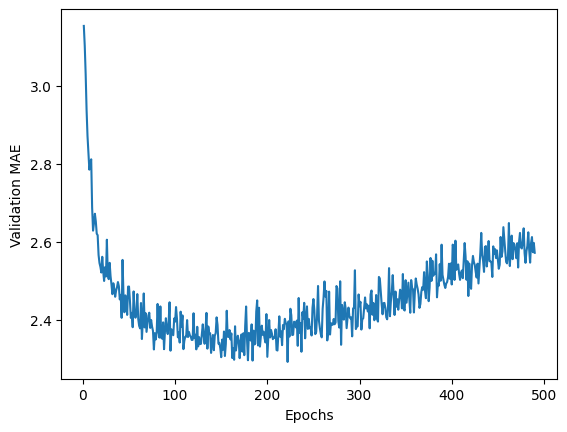
\includegraphics{chapters/09_pandas_line_graphs/pandas_line_graphs_files/figure-pdf/cell-15-output-1.png}

}

\end{figure}

Notice that when there is a market downturn, there is a spike in the
realized volatility graph.

\hypertarget{implied-volatility---the-vix-index}{%
\section{Implied Volatility - The VIX
Index}\label{implied-volatility---the-vix-index}}

During times of market stress, options all become more expensive. One
measure of the relative cheapness or expensiveness of options is
\emph{implied volatility}. When options become more expensive, implied
volatility rises.

One of the complexities of implied volatility measurements is that even
for a single underlying they differ depending on strike and expiration.
However, all implied volatility measurements tend to rise and fall
together.

The VIX index is a single number that summarizes the general level of
option implied volatility for options on the S\&P500. The S\&P500
represents a large number of the most important stocks in America.
Moreover, S\&P500 options are the most actively traded options in the
world. For these reasons, the VIX is a good barometer for overall
implied volatility level in the stock market.

Let's plot \texttt{vix} along side the other volatility measures in the
same graph.

\begin{Shaded}
\begin{Highlighting}[]
\NormalTok{df\_spy.plot(x}\OperatorTok{=}\StringTok{\textquotesingle{}date\textquotesingle{}}\NormalTok{, y}\OperatorTok{=}\NormalTok{[}\StringTok{\textquotesingle{}spy\textquotesingle{}}\NormalTok{, }\StringTok{\textquotesingle{}return\textquotesingle{}}\NormalTok{, }\StringTok{\textquotesingle{}realized\_vol\textquotesingle{}}\NormalTok{, }\StringTok{\textquotesingle{}vix\textquotesingle{}}\NormalTok{,], subplots}\OperatorTok{=}\VariableTok{True}\NormalTok{, style}\OperatorTok{=}\StringTok{\textquotesingle{}k\textquotesingle{}}\NormalTok{, grid}\OperatorTok{=}\VariableTok{True}\NormalTok{, alpha}\OperatorTok{=}\FloatTok{0.75}\NormalTok{, figsize}\OperatorTok{=}\NormalTok{(}\DecValTok{8}\NormalTok{, }\DecValTok{16}\NormalTok{))}\OperatorTok{;}
\end{Highlighting}
\end{Shaded}

\begin{figure}[H]

{\centering 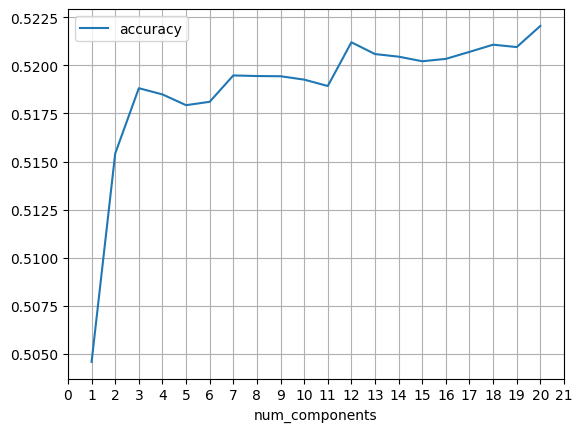
\includegraphics{chapters/09_pandas_line_graphs/pandas_line_graphs_files/figure-pdf/cell-16-output-1.png}

}

\end{figure}

This plot demonstrates typical behavior of stock market returns and
volatility: when there is a market downturn, there is a spike in both
implied volatility and realized volatility.

\hypertarget{further-reading-1}{%
\section{Further Reading}\label{further-reading-1}}

\emph{Python Data Science Handbook (VanderPlas)} - Section 1.3 - Python
Magic Commands

\emph{Python for Finance (Hilpisch)} - Section 6.2 - Financial Data

\emph{Python for Data Analysis (McKinney)} - Section 8.1 - A Brief
\textbf{matplotlib} API Primer

\emph{Python for Data Analysis (McKinney)} - Section 8.2 - Plotting
Functions in \textbf{pandas}

\hypertarget{bar-charts-with-pandas}{%
\chapter{\texorpdfstring{Bar Charts with
\textbf{pandas}}{Bar Charts with pandas}}\label{bar-charts-with-pandas}}

The purpose of this chapter is to demonstrate how to easily generate bar
charts with the \textbf{pandas} built-in \texttt{.plot()} function.

We apply this technique to the task of visualizing monthly pnls for the
data set in the \texttt{spy\_2018\_call\_pnl.csv} data file.

\hypertarget{load-packages-1}\NormalTok{matplotlib inline}
\end{Highlighting}
\end{Shaded}

\textbf{Knowledge Challenge:} What is the purpose of this line of code
in the above cell: \texttt{\%matplotlib\ inline}?

\begin{Shaded}
\begin{Highlighting}[]
\CommentTok{\# plotting graphs below code cells}
\end{Highlighting}
\end{Shaded}

\hypertarget{reading-in-data-8}{%
\section{Reading-In Data}\label{reading-in-data-8}}

Next, let's read in the data from the CSV file.

\begin{Shaded}
\begin{Highlighting}[]
\NormalTok{df\_pnl }\OperatorTok{=}\NormalTok{ pd.read\_csv(}\StringTok{\textquotesingle{}spy\_2018\_call\_pnl.csv\textquotesingle{}}\NormalTok{)}
\NormalTok{df\_pnl.head()}
\end{Highlighting}
\end{Shaded}

\begin{longtable}[]{@{}lllllllllllll@{}}
\toprule\noalign{}
& underlying & upx & type & expiration & data\_date & strike & bid & ask
& implied\_vol & delta & dly\_opt\_pnl & dly\_dh\_pnl \\
\midrule\noalign{}
\endhead
\bottomrule\noalign{}
\endlastfoot
0 & SPY & 266.529999 & call & 2018-01-19 & 2017-12-15 & 270 & 1.14 &
1.16 & 0.068257 & 0.328344 & -0.02 & 0.000000 \\
1 & SPY & 268.230011 & call & 2018-01-19 & 2017-12-18 & 270 & 1.68 &
1.69 & 0.071450 & 0.421353 & -0.53 & 0.558189 \\
2 & SPY & 267.250000 & call & 2018-01-19 & 2017-12-19 & 270 & 1.39 &
1.41 & 0.074841 & 0.365808 & 0.28 & -0.412931 \\
3 & SPY & 267.100006 & call & 2018-01-19 & 2017-12-20 & 270 & 1.10 &
1.11 & 0.070911 & 0.327058 & 0.30 & -0.054869 \\
4 & SPY & 267.540009 & call & 2018-01-19 & 2017-12-21 & 270 & 1.31 &
1.32 & 0.072183 & 0.372113 & -0.21 & 0.143906 \\
\end{longtable}

This data consists of daily PNLs from 12 different SPY short call trades
throughout 2018.

\hypertarget{wrangling}{%
\section{Wrangling}\label{wrangling}}

First, we will refactor the \texttt{expiration} and \texttt{data\_date}
columns to \texttt{datetime} using the \texttt{pd.to\_datetime()}
method.

\begin{Shaded}
\begin{Highlighting}[]
\NormalTok{df\_pnl[}\StringTok{\textquotesingle{}expiration\textquotesingle{}}\NormalTok{] }\OperatorTok{=}\NormalTok{ pd.to\_datetime(df\_pnl[}\StringTok{\textquotesingle{}expiration\textquotesingle{}}\NormalTok{])}
\NormalTok{df\_pnl[}\StringTok{\textquotesingle{}data\_date\textquotesingle{}}\NormalTok{] }\OperatorTok{=}\NormalTok{ pd.to\_datetime(df\_pnl[}\StringTok{\textquotesingle{}data\_date\textquotesingle{}}\NormalTok{])}
\NormalTok{df\_pnl.head()}
\end{Highlighting}
\end{Shaded}

\begin{longtable}[]{@{}lllllllllllll@{}}
\toprule\noalign{}
& underlying & upx & type & expiration & data\_date & strike & bid & ask
& implied\_vol & delta & dly\_opt\_pnl & dly\_dh\_pnl \\
\midrule\noalign{}
\endhead
\bottomrule\noalign{}
\endlastfoot
0 & SPY & 266.529999 & call & 2018-01-19 & 2017-12-15 & 270 & 1.14 &
1.16 & 0.068257 & 0.328344 & -0.02 & 0.000000 \\
1 & SPY & 268.230011 & call & 2018-01-19 & 2017-12-18 & 270 & 1.68 &
1.69 & 0.071450 & 0.421353 & -0.53 & 0.558189 \\
2 & SPY & 267.250000 & call & 2018-01-19 & 2017-12-19 & 270 & 1.39 &
1.41 & 0.074841 & 0.365808 & 0.28 & -0.412931 \\
3 & SPY & 267.100006 & call & 2018-01-19 & 2017-12-20 & 270 & 1.10 &
1.11 & 0.070911 & 0.327058 & 0.30 & -0.054869 \\
4 & SPY & 267.540009 & call & 2018-01-19 & 2017-12-21 & 270 & 1.31 &
1.32 & 0.072183 & 0.372113 & -0.21 & 0.143906 \\
\end{longtable}

We are interested in total pnl, which is the sum of the option pnl and
the delta-hedge PNL. Let's add a column called \texttt{dly\_tot\_pnl}
which captures this logic.

\begin{Shaded}
\begin{Highlighting}[]
\NormalTok{df\_pnl[}\StringTok{\textquotesingle{}dly\_tot\_pnl\textquotesingle{}}\NormalTok{] }\OperatorTok{=}\NormalTok{ df\_pnl[}\StringTok{\textquotesingle{}dly\_opt\_pnl\textquotesingle{}}\NormalTok{] }\OperatorTok{+}\NormalTok{ df\_pnl[}\StringTok{\textquotesingle{}dly\_dh\_pnl\textquotesingle{}}\NormalTok{]}
\NormalTok{df\_pnl.head()}
\end{Highlighting}
\end{Shaded}

\begin{longtable}[]{@{}llllllllllllll@{}}
\toprule\noalign{}
& underlying & upx & type & expiration & data\_date & strike & bid & ask
& implied\_vol & delta & dly\_opt\_pnl & dly\_dh\_pnl & dly\_tot\_pnl \\
\midrule\noalign{}
\endhead
\bottomrule\noalign{}
\endlastfoot
0 & SPY & 266.529999 & call & 2018-01-19 & 2017-12-15 & 270 & 1.14 &
1.16 & 0.068257 & 0.328344 & -0.02 & 0.000000 & -0.020000 \\
1 & SPY & 268.230011 & call & 2018-01-19 & 2017-12-18 & 270 & 1.68 &
1.69 & 0.071450 & 0.421353 & -0.53 & 0.558189 & 0.028189 \\
2 & SPY & 267.250000 & call & 2018-01-19 & 2017-12-19 & 270 & 1.39 &
1.41 & 0.074841 & 0.365808 & 0.28 & -0.412931 & -0.132931 \\
3 & SPY & 267.100006 & call & 2018-01-19 & 2017-12-20 & 270 & 1.10 &
1.11 & 0.070911 & 0.327058 & 0.30 & -0.054869 & 0.245131 \\
4 & SPY & 267.540009 & call & 2018-01-19 & 2017-12-21 & 270 & 1.31 &
1.32 & 0.072183 & 0.372113 & -0.21 & 0.143906 & -0.066094 \\
\end{longtable}

As the final step of our wrangling, let's extract the \texttt{year} and
\texttt{month} of the \texttt{expiration}, as this is what we will use
for grouping.

\begin{Shaded}
\begin{Highlighting}[]
\NormalTok{df\_pnl[}\StringTok{\textquotesingle{}year\textquotesingle{}}\NormalTok{] }\OperatorTok{=}\NormalTok{ df\_pnl[}\StringTok{\textquotesingle{}expiration\textquotesingle{}}\NormalTok{].dt.year}
\NormalTok{df\_pnl[}\StringTok{\textquotesingle{}month\textquotesingle{}}\NormalTok{] }\OperatorTok{=}\NormalTok{ df\_pnl[}\StringTok{\textquotesingle{}expiration\textquotesingle{}}\NormalTok{].dt.month}
\NormalTok{df\_pnl.head()}
\end{Highlighting}
\end{Shaded}

\begin{longtable}[]{@{}llllllllllllllll@{}}
\toprule\noalign{}
& underlying & upx & type & expiration & data\_date & strike & bid & ask
& implied\_vol & delta & dly\_opt\_pnl & dly\_dh\_pnl & dly\_tot\_pnl &
year & month \\
\midrule\noalign{}
\endhead
\bottomrule\noalign{}
\endlastfoot
0 & SPY & 266.529999 & call & 2018-01-19 & 2017-12-15 & 270 & 1.14 &
1.16 & 0.068257 & 0.328344 & -0.02 & 0.000000 & -0.020000 & 2018 & 1 \\
1 & SPY & 268.230011 & call & 2018-01-19 & 2017-12-18 & 270 & 1.68 &
1.69 & 0.071450 & 0.421353 & -0.53 & 0.558189 & 0.028189 & 2018 & 1 \\
2 & SPY & 267.250000 & call & 2018-01-19 & 2017-12-19 & 270 & 1.39 &
1.41 & 0.074841 & 0.365808 & 0.28 & -0.412931 & -0.132931 & 2018 & 1 \\
3 & SPY & 267.100006 & call & 2018-01-19 & 2017-12-20 & 270 & 1.10 &
1.11 & 0.070911 & 0.327058 & 0.30 & -0.054869 & 0.245131 & 2018 & 1 \\
4 & SPY & 267.540009 & call & 2018-01-19 & 2017-12-21 & 270 & 1.31 &
1.32 & 0.072183 & 0.372113 & -0.21 & 0.143906 & -0.066094 & 2018 & 1 \\
\end{longtable}

\hypertarget{groupby-and-agg}{%
\section{\texorpdfstring{\texttt{groupby()} and
\texttt{agg()}}{groupby() and agg()}}\label{groupby-and-agg}}

We are interested in graphing the PNLs by expiration, so let's sum up
the \texttt{dly\_tot\_pnl} by the year and month of the expiration.

\begin{Shaded}
\begin{Highlighting}[]
\NormalTok{df\_monthly }\OperatorTok{=} \OperatorTok{\textbackslash{}}
\NormalTok{    df\_pnl.groupby([}\StringTok{\textquotesingle{}year\textquotesingle{}}\NormalTok{, }\StringTok{\textquotesingle{}month\textquotesingle{}}\NormalTok{])[}\StringTok{\textquotesingle{}dly\_tot\_pnl\textquotesingle{}}\NormalTok{].agg([np.}\BuiltInTok{sum}\NormalTok{]).reset\_index()}
\NormalTok{df\_monthly.head()}
\end{Highlighting}
\end{Shaded}

\begin{longtable}[]{@{}llll@{}}
\toprule\noalign{}
& year & month & sum \\
\midrule\noalign{}
\endhead
\bottomrule\noalign{}
\endlastfoot
0 & 2018 & 1 & 0.091963 \\
1 & 2018 & 2 & -2.759090 \\
2 & 2018 & 3 & -0.340270 \\
3 & 2018 & 4 & -1.174222 \\
4 & 2018 & 5 & 1.487206 \\
\end{longtable}

Before we proceed to graphing, let's change the name of the aggregated
pnl column to something more meaningful.

\begin{Shaded}
\begin{Highlighting}[]
\NormalTok{df\_monthly.rename(columns}\OperatorTok{=}\NormalTok{\{}\StringTok{\textquotesingle{}sum\textquotesingle{}}\NormalTok{:}\StringTok{\textquotesingle{}monthly\_pnl\textquotesingle{}}\NormalTok{\}, inplace}\OperatorTok{=}\VariableTok{True}\NormalTok{)}
\end{Highlighting}
\end{Shaded}

\hypertarget{visualizing-the-data}{%
\section{Visualizing the Data}\label{visualizing-the-data}}

Creating a simple bar graph of the \texttt{monthly\_pnls} in
\texttt{df\_monthly} can be done easily with a single line of code.

\begin{Shaded}
\begin{Highlighting}[]
\NormalTok{df\_monthly.plot(x}\OperatorTok{=}\StringTok{\textquotesingle{}month\textquotesingle{}}\NormalTok{, y}\OperatorTok{=}\StringTok{\textquotesingle{}monthly\_pnl\textquotesingle{}}\NormalTok{, kind}\OperatorTok{=}\StringTok{\textquotesingle{}bar\textquotesingle{}}\NormalTok{)}\OperatorTok{;}
\end{Highlighting}
\end{Shaded}

\begin{figure}[H]

{\centering \includegraphics{chapters/10_pandas_bar_charts/pandas_bar_charts_files/figure-pdf/cell-10-output-1.png}

}

\end{figure}

While the above graph may be fine for EDA purposes, it still leaves much
to be desired, especially if our intention is to share it with a broader
audience.

The following code makes several of modifications to improve its
appearance.

\begin{Shaded}
\begin{Highlighting}[]
\NormalTok{ax }\OperatorTok{=} \OperatorTok{\textbackslash{}}
\NormalTok{    df\_monthly.}\OperatorTok{\textbackslash{}}
\NormalTok{        plot(}
\NormalTok{            x }\OperatorTok{=} \StringTok{\textquotesingle{}month\textquotesingle{}}\NormalTok{,}
\NormalTok{            y }\OperatorTok{=} \StringTok{\textquotesingle{}monthly\_pnl\textquotesingle{}}\NormalTok{,}
\NormalTok{            kind}\OperatorTok{=}\StringTok{\textquotesingle{}bar\textquotesingle{}}\NormalTok{,}
\NormalTok{            color}\OperatorTok{=}\StringTok{\textquotesingle{}k\textquotesingle{}}\NormalTok{, }\CommentTok{\# color is grey}
\NormalTok{            grid}\OperatorTok{=}\VariableTok{True}\NormalTok{ , }\CommentTok{\# adding a grid}
\NormalTok{            alpha}\OperatorTok{=}\FloatTok{0.75}\NormalTok{, }\CommentTok{\# translucence}
\NormalTok{            width}\OperatorTok{=}\FloatTok{0.8}\NormalTok{, }\CommentTok{\# increasing the width of the bars}
\NormalTok{            title}\OperatorTok{=}\StringTok{\textquotesingle{}Monthly PNL for SPY Calls\textquotesingle{}}\NormalTok{,}
\NormalTok{            figsize}\OperatorTok{=}\NormalTok{(}\DecValTok{8}\NormalTok{, }\DecValTok{4}\NormalTok{), }\CommentTok{\# modifying the figure size}
\NormalTok{        )}\OperatorTok{;}

\NormalTok{ax.set\_xlabel(}\StringTok{"Month"}\NormalTok{)}\OperatorTok{;} \CommentTok{\# x axis label}
\NormalTok{ax.set\_ylabel(}\StringTok{"PNL"}\NormalTok{)}\OperatorTok{;}   \CommentTok{\# y axis label}
\end{Highlighting}
\end{Shaded}

\begin{figure}[H]

{\centering 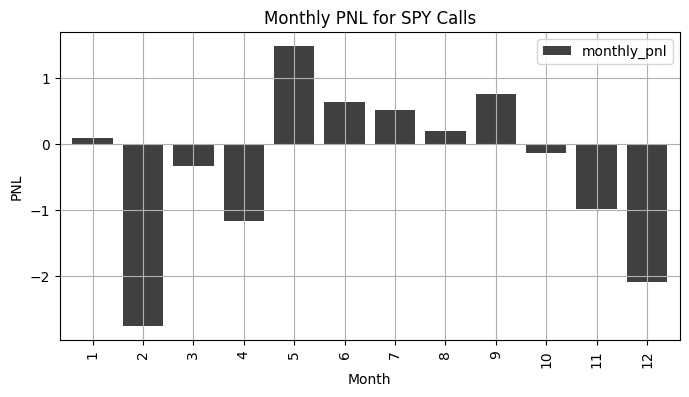
\includegraphics{chapters/10_pandas_bar_charts/pandas_bar_charts_files/figure-pdf/cell-11-output-1.png}

}

\end{figure}

\begin{center}\rule{0.5\linewidth}{0.5pt}\end{center}

\textbf{Code Challenge:} Google and try to find how you create a
\emph{horizontal} bar graph using \textbf{pandas}.

\begin{Shaded}
\begin{Highlighting}[]
\NormalTok{ax }\OperatorTok{=} \OperatorTok{\textbackslash{}}
\NormalTok{    df\_monthly.}\OperatorTok{\textbackslash{}}
\NormalTok{        plot(}
\NormalTok{            x }\OperatorTok{=} \StringTok{\textquotesingle{}month\textquotesingle{}}\NormalTok{,}
\NormalTok{            y }\OperatorTok{=} \StringTok{\textquotesingle{}monthly\_pnl\textquotesingle{}}\NormalTok{,}
\NormalTok{            kind}\OperatorTok{=}\StringTok{\textquotesingle{}barh\textquotesingle{}}\NormalTok{, }\CommentTok{\# changed to barh}
\NormalTok{            color}\OperatorTok{=}\StringTok{\textquotesingle{}k\textquotesingle{}}\NormalTok{, }\CommentTok{\# color is grey}
\NormalTok{            grid}\OperatorTok{=}\VariableTok{True}\NormalTok{ , }\CommentTok{\# adding a grid}
\NormalTok{            alpha}\OperatorTok{=}\FloatTok{0.75}\NormalTok{, }\CommentTok{\# translucence}
\NormalTok{            width}\OperatorTok{=}\FloatTok{0.8}\NormalTok{, }\CommentTok{\# increasing the width of the bars}
\NormalTok{            title}\OperatorTok{=}\StringTok{\textquotesingle{}Monthly PNL for SPY Calls\textquotesingle{}}\NormalTok{,}
\NormalTok{            figsize}\OperatorTok{=}\NormalTok{(}\DecValTok{8}\NormalTok{, }\DecValTok{4}\NormalTok{), }\CommentTok{\# modifying the figure size}
\NormalTok{        )}\OperatorTok{;}

\NormalTok{ax.set\_xlabel(}\StringTok{"Month"}\NormalTok{)}\OperatorTok{;} \CommentTok{\# x axis label}
\NormalTok{ax.set\_ylabel(}\StringTok{"PNL"}\NormalTok{)}\OperatorTok{;} 
\end{Highlighting}
\end{Shaded}

\begin{figure}[H]

{\centering \includegraphics{chapters/10_pandas_bar_charts/pandas_bar_charts_files/figure-pdf/cell-12-output-1.png}

}

\end{figure}

\begin{center}\rule{0.5\linewidth}{0.5pt}\end{center}

\hypertarget{a-few-words-about-visualization}{%
\section{A Few Words About
Visualization}\label{a-few-words-about-visualization}}

Visualizing data can be an effective way of communicating results to
others, or exploring data on your own. The benefit of visualization
comes into focus when we can convey a particular result more quickly and
more viscerally with a graph rather than a table of numbers.

This is nicely illustrated by comparing our bar graph to the original
\texttt{DataFrame} of data. Consider the following question:

\emph{What were the two worst PNL months for these SPY calls?}

Do you find it easier to answer the question using the bar graph or the
table? Explain why.

\begin{Shaded}
\begin{Highlighting}[]
\NormalTok{ax }\OperatorTok{=} \OperatorTok{\textbackslash{}}
\NormalTok{    df\_monthly.}\OperatorTok{\textbackslash{}}
\NormalTok{        plot(}
\NormalTok{            x }\OperatorTok{=} \StringTok{\textquotesingle{}month\textquotesingle{}}\NormalTok{,}
\NormalTok{            y }\OperatorTok{=} \StringTok{\textquotesingle{}monthly\_pnl\textquotesingle{}}\NormalTok{,}
\NormalTok{            kind }\OperatorTok{=} \StringTok{\textquotesingle{}bar\textquotesingle{}}\NormalTok{, }
\NormalTok{            color}\OperatorTok{=}\StringTok{\textquotesingle{}k\textquotesingle{}}\NormalTok{, }\CommentTok{\# color is grey}
\NormalTok{            grid}\OperatorTok{=}\VariableTok{True}\NormalTok{, }\CommentTok{\# adding a grid}
\NormalTok{            alpha}\OperatorTok{=}\FloatTok{0.75}\NormalTok{, }\CommentTok{\# translucence}
\NormalTok{            width}\OperatorTok{=}\FloatTok{0.8}\NormalTok{, }\CommentTok{\# increasing the width of the bars}
\NormalTok{            title}\OperatorTok{=}\StringTok{\textquotesingle{}Monthly PNL for SPY Calls\textquotesingle{}}\NormalTok{,}
\NormalTok{            figsize}\OperatorTok{=}\NormalTok{(}\DecValTok{8}\NormalTok{, }\DecValTok{4}\NormalTok{), }\CommentTok{\# modifying the figure size}
\NormalTok{        )}\OperatorTok{;}

\NormalTok{ax.set\_xlabel(}\StringTok{"Month"}\NormalTok{)}\OperatorTok{;} \CommentTok{\# x axis label}
\NormalTok{ax.set\_ylabel(}\StringTok{"PNL"}\NormalTok{)}\OperatorTok{;}   \CommentTok{\# y axis label}
\end{Highlighting}
\end{Shaded}

\begin{figure}[H]

{\centering \includegraphics{chapters/10_pandas_bar_charts/pandas_bar_charts_files/figure-pdf/cell-13-output-1.png}

}

\end{figure}

\begin{Shaded}
\begin{Highlighting}[]
\NormalTok{df\_monthly}
\end{Highlighting}
\end{Shaded}

\begin{longtable}[]{@{}llll@{}}
\toprule\noalign{}
& year & month & monthly\_pnl \\
\midrule\noalign{}
\endhead
\bottomrule\noalign{}
\endlastfoot
0 & 2018 & 1 & 0.091963 \\
1 & 2018 & 2 & -2.759090 \\
2 & 2018 & 3 & -0.340270 \\
3 & 2018 & 4 & -1.174222 \\
4 & 2018 & 5 & 1.487206 \\
5 & 2018 & 6 & 0.644469 \\
6 & 2018 & 7 & 0.516556 \\
7 & 2018 & 8 & 0.195526 \\
8 & 2018 & 9 & 0.753701 \\
9 & 2018 & 10 & -0.133537 \\
10 & 2018 & 11 & -0.979537 \\
11 & 2018 & 12 & -2.085526 \\
\end{longtable}

\hypertarget{related-reading-7}{%
\section{Related Reading}\label{related-reading-7}}

\emph{Python for Data Analysis (McKinney)} - Section 8.2 - Plotting
Functions in \textbf{pandas}

\hypertarget{scatter-plots-with-pandas}{%
\chapter{\texorpdfstring{Scatter Plots with
\textbf{pandas}}{Scatter Plots with pandas}}\label{scatter-plots-with-pandas}}

The purpose of this chapter is to demonstrate the \textbf{pandas}
built-in functionality for creating scatter plots.

The financial task we will accomplish is demonstrating SPY's
\emph{implied leverage effect}: when the market suffers losses, implied
volatility increases; when the market experiences gains, implied
volatility decreases.

Our measure of SPY implied volatility will be the VIX index. To verify
the above relationship, we will plot SPY daily returns against daily
changes in the VIX for 2016Q1-2021Q2.

\hypertarget{loading-packages-4}\NormalTok{matplotlib inline}
\end{Highlighting}
\end{Shaded}

\hypertarget{reading-in-data-9}{%
\section{Reading-In Data}\label{reading-in-data-9}}

Next, let's use \textbf{pandas\_datareader} to read in the SPY and VIX
data.

\begin{Shaded}
\begin{Highlighting}[]
\NormalTok{df\_spy }\OperatorTok{=}\NormalTok{ pdr.get\_data\_yahoo([}\StringTok{\textquotesingle{}SPY\textquotesingle{}}\NormalTok{, }\StringTok{\textquotesingle{}\^{}VIX\textquotesingle{}}\NormalTok{], start}\OperatorTok{=}\StringTok{\textquotesingle{}2016{-}01{-}01\textquotesingle{}}\NormalTok{, end}\OperatorTok{=}\StringTok{\textquotesingle{}2021{-}06{-}30\textquotesingle{}}\NormalTok{)}
\NormalTok{df\_spy }\OperatorTok{=}\NormalTok{ df\_spy.}\BuiltInTok{round}\NormalTok{(}\DecValTok{2}\NormalTok{)}
\NormalTok{df\_spy.head()}
\end{Highlighting}
\end{Shaded}

\begin{verbatim}
[*********************100%***********************]  2 of 2 completed
\end{verbatim}

\begin{longtable}[]{@{}lllllllllllll@{}}
\toprule\noalign{}
&
\multicolumn{2}{>{\raggedright\arraybackslash}p{(\columnwidth - 24\tabcolsep) * \real{0.0000} + 2\tabcolsep}}{%
Adj Close} &
\multicolumn{2}{>{\raggedright\arraybackslash}p{(\columnwidth - 24\tabcolsep) * \real{0.0000} + 2\tabcolsep}}{%
Close} &
\multicolumn{2}{>{\raggedright\arraybackslash}p{(\columnwidth - 24\tabcolsep) * \real{0.0000} + 2\tabcolsep}}{%
High} &
\multicolumn{2}{>{\raggedright\arraybackslash}p{(\columnwidth - 24\tabcolsep) * \real{0.0000} + 2\tabcolsep}}{%
Low} &
\multicolumn{2}{>{\raggedright\arraybackslash}p{(\columnwidth - 24\tabcolsep) * \real{0.0000} + 2\tabcolsep}}{%
Open} &
\multicolumn{2}{>{\raggedright\arraybackslash}p{(\columnwidth - 24\tabcolsep) * \real{0.0000} + 2\tabcolsep}@{}}{%
Volume} \\
& SPY & \^{}VIX & SPY & \^{}VIX & SPY & \^{}VIX & SPY & \^{}VIX & SPY &
\^{}VIX & SPY & \^{}VIX \\
Date & & & & & & & & & & & & \\
\midrule\noalign{}
\endhead
\bottomrule\noalign{}
\endlastfoot
2016-01-04 & 175.91 & 20.70 & 201.02 & 20.70 & 201.03 & 23.36 & 198.59 &
20.67 & 200.49 & 22.48 & 222353500 & 0 \\
2016-01-05 & 176.21 & 19.34 & 201.36 & 19.34 & 201.90 & 21.06 & 200.05 &
19.25 & 201.40 & 20.75 & 110845800 & 0 \\
2016-01-06 & 173.98 & 20.59 & 198.82 & 20.59 & 200.06 & 21.86 & 197.60 &
19.80 & 198.34 & 21.67 & 152112600 & 0 \\
2016-01-07 & 169.81 & 24.99 & 194.05 & 24.99 & 197.44 & 25.86 & 193.59 &
22.40 & 195.33 & 23.22 & 213436100 & 0 \\
2016-01-08 & 167.95 & 27.01 & 191.92 & 27.01 & 195.85 & 27.08 & 191.58 &
22.48 & 195.19 & 22.96 & 209817200 & 0 \\
\end{longtable}

The following code cleans up the data by isolating the the
\texttt{Close} prices, resetting the index, and then changing the column
names

\begin{Shaded}
\begin{Highlighting}[]
\NormalTok{df\_spy }\OperatorTok{=}\NormalTok{ df\_spy[}\StringTok{\textquotesingle{}Close\textquotesingle{}}\NormalTok{].reset\_index()}
\NormalTok{df\_spy.rename(columns}\OperatorTok{=}\NormalTok{\{}\StringTok{\textquotesingle{}Date\textquotesingle{}}\NormalTok{:}\StringTok{\textquotesingle{}date\textquotesingle{}}\NormalTok{,}\StringTok{\textquotesingle{}SPY\textquotesingle{}}\NormalTok{:}\StringTok{\textquotesingle{}spy\textquotesingle{}}\NormalTok{,}\StringTok{\textquotesingle{}\^{}VIX\textquotesingle{}}\NormalTok{:}\StringTok{\textquotesingle{}vix\textquotesingle{}}\NormalTok{\}, inplace}\OperatorTok{=}\VariableTok{True}\NormalTok{)}
\NormalTok{df\_spy.head()}
\end{Highlighting}
\end{Shaded}

\begin{longtable}[]{@{}llll@{}}
\toprule\noalign{}
& date & spy & vix \\
\midrule\noalign{}
\endhead
\bottomrule\noalign{}
\endlastfoot
0 & 2016-01-04 & 201.02 & 20.70 \\
1 & 2016-01-05 & 201.36 & 19.34 \\
2 & 2016-01-06 & 198.82 & 20.59 \\
3 & 2016-01-07 & 194.05 & 24.99 \\
4 & 2016-01-08 & 191.92 & 27.01 \\
\end{longtable}

\hypertarget{adding-returns-and-vix-changes-to-df_spy}{%
\section{\texorpdfstring{Adding Returns and VIX Changes to
\texttt{df\_spy}}{Adding Returns and VIX Changes to df\_spy}}\label{adding-returns-and-vix-changes-to-df_spy}}

Let's add a \texttt{return} column to \texttt{df\_spy}.

\begin{Shaded}
\begin{Highlighting}[]
\NormalTok{df\_spy[}\StringTok{\textquotesingle{}return\textquotesingle{}}\NormalTok{] }\OperatorTok{=}\NormalTok{ df\_spy[}\StringTok{\textquotesingle{}spy\textquotesingle{}}\NormalTok{] }\OperatorTok{/}\NormalTok{ df\_spy[}\StringTok{\textquotesingle{}spy\textquotesingle{}}\NormalTok{].shift(}\DecValTok{1}\NormalTok{) }\OperatorTok{{-}} \DecValTok{1}
\NormalTok{df\_spy.head()}
\end{Highlighting}
\end{Shaded}

\begin{longtable}[]{@{}lllll@{}}
\toprule\noalign{}
& date & spy & vix & return \\
\midrule\noalign{}
\endhead
\bottomrule\noalign{}
\endlastfoot
0 & 2016-01-04 & 201.02 & 20.70 & NaN \\
1 & 2016-01-05 & 201.36 & 19.34 & 0.001691 \\
2 & 2016-01-06 & 198.82 & 20.59 & -0.012614 \\
3 & 2016-01-07 & 194.05 & 24.99 & -0.023992 \\
4 & 2016-01-08 & 191.92 & 27.01 & -0.010977 \\
\end{longtable}

Next, let's calculate the daily change in the VIX, and put it in a new
column called \texttt{vix\_chg}.

\begin{Shaded}
\begin{Highlighting}[]
\NormalTok{df\_spy[}\StringTok{\textquotesingle{}vix\_chng\textquotesingle{}}\NormalTok{] }\OperatorTok{=}\NormalTok{ df\_spy[}\StringTok{\textquotesingle{}vix\textquotesingle{}}\NormalTok{].diff()}
\NormalTok{df\_spy.head()}
\end{Highlighting}
\end{Shaded}

\begin{longtable}[]{@{}llllll@{}}
\toprule\noalign{}
& date & spy & vix & return & vix\_chng \\
\midrule\noalign{}
\endhead
\bottomrule\noalign{}
\endlastfoot
0 & 2016-01-04 & 201.02 & 20.70 & NaN & NaN \\
1 & 2016-01-05 & 201.36 & 19.34 & 0.001691 & -1.36 \\
2 & 2016-01-06 & 198.82 & 20.59 & -0.012614 & 1.25 \\
3 & 2016-01-07 & 194.05 & 24.99 & -0.023992 & 4.40 \\
4 & 2016-01-08 & 191.92 & 27.01 & -0.010977 & 2.02 \\
\end{longtable}

The \texttt{return} column in \texttt{df\_spy} is expressed as a
decimal, so let's change the \texttt{vix} and \texttt{vix\_chng} columns
of \texttt{df\_vix} to also be expressed as decimals.

\begin{Shaded}
\begin{Highlighting}[]
\NormalTok{df\_spy[}\StringTok{\textquotesingle{}vix\textquotesingle{}}\NormalTok{] }\OperatorTok{=}\NormalTok{ df\_spy[}\StringTok{\textquotesingle{}vix\textquotesingle{}}\NormalTok{] }\OperatorTok{/} \DecValTok{100}
\NormalTok{df\_spy[}\StringTok{\textquotesingle{}vix\_chng\textquotesingle{}}\NormalTok{] }\OperatorTok{=}\NormalTok{ df\_spy[}\StringTok{\textquotesingle{}vix\_chng\textquotesingle{}}\NormalTok{] }\OperatorTok{/} \DecValTok{100}
\NormalTok{df\_spy.head()}
\end{Highlighting}
\end{Shaded}

\begin{longtable}[]{@{}llllll@{}}
\toprule\noalign{}
& date & spy & vix & return & vix\_chng \\
\midrule\noalign{}
\endhead
\bottomrule\noalign{}
\endlastfoot
0 & 2016-01-04 & 201.02 & 0.2070 & NaN & NaN \\
1 & 2016-01-05 & 201.36 & 0.1934 & 0.001691 & -0.0136 \\
2 & 2016-01-06 & 198.82 & 0.2059 & -0.012614 & 0.0125 \\
3 & 2016-01-07 & 194.05 & 0.2499 & -0.023992 & 0.0440 \\
4 & 2016-01-08 & 191.92 & 0.2701 & -0.010977 & 0.0202 \\
\end{longtable}

\hypertarget{scatter-plot}{%
\section{Scatter Plot}\label{scatter-plot}}

Now that we have our data wrangled, we are in position to use the
\texttt{DataFrame.plot.scatter()} method to plot daily SPY return
against daily changes in the VIX.

\begin{Shaded}
\begin{Highlighting}[]
\NormalTok{df\_spy.plot.scatter(}\StringTok{\textquotesingle{}return\textquotesingle{}}\NormalTok{, }\StringTok{\textquotesingle{}vix\_chng\textquotesingle{}}\NormalTok{)}\OperatorTok{;}
\end{Highlighting}
\end{Shaded}

\begin{figure}[H]

{\centering \includegraphics{chapters/11_pandas_scatter_plots/pandas_scatter_plots_files/figure-pdf/cell-8-output-1.png}

}

\end{figure}

The following code improves the aesthetics of our plot:

\begin{Shaded}
\begin{Highlighting}[]
\NormalTok{df\_spy.plot.scatter(}
\NormalTok{    x }\OperatorTok{=} \StringTok{\textquotesingle{}return\textquotesingle{}}\NormalTok{,}
\NormalTok{    y }\OperatorTok{=} \StringTok{\textquotesingle{}vix\_chng\textquotesingle{}}\NormalTok{,}
\NormalTok{    grid}\OperatorTok{=}\VariableTok{True}\NormalTok{ ,  }
\NormalTok{    c}\OperatorTok{=}\StringTok{\textquotesingle{}k\textquotesingle{}}\NormalTok{,}
\NormalTok{    alpha}\OperatorTok{=}\FloatTok{0.75}\NormalTok{,}
\NormalTok{    s}\OperatorTok{=}\DecValTok{10}\NormalTok{,  }\CommentTok{\# changing the size of the dots}
\NormalTok{    figsize}\OperatorTok{=}\NormalTok{(}\DecValTok{8}\NormalTok{, }\DecValTok{6}\NormalTok{),}
\NormalTok{    title}\OperatorTok{=}\StringTok{\textquotesingle{}SPY Return vs VIX Changes (2016Q1{-}2021Q2: daily)\textquotesingle{}}\NormalTok{,}
\NormalTok{)}\OperatorTok{;}
\end{Highlighting}
\end{Shaded}

\begin{figure}[H]

{\centering \includegraphics{chapters/11_pandas_scatter_plots/pandas_scatter_plots_files/figure-pdf/cell-9-output-1.png}

}

\end{figure}

\hypertarget{visualization-with-seaborn}{%
\chapter{\texorpdfstring{Visualization with
\textbf{seaborn}}{Visualization with seaborn}}\label{visualization-with-seaborn}}

In the previous visualization we used the built-in plotting capabilities
of \textbf{pandas} to create some useful financial graphs. In this
tutorial, we recreate those plots using the \textbf{seaborn}
visualization package.

Like the \textbf{pandas} visualization functionality, \textbf{seaborn}
is built on top of the \textbf{matplotlib} package. As previously
discussed, \textbf{matplotlib} allows for low level control over
visualizations, which makes it very flexible. However, this flexibility
comes at the cost of complexity. In contrast, \textbf{seaborn} provides
a high level interface that allows for easy implementations of
attractive graphs.

The focus of \textbf{seaborn} is general statistical data
visualizations, whereas \textbf{pandas} is more tailor-made for
financial time series.

This tutorial is not meant to be a comprehensive introduction to
\textbf{seaborn}. Rather, my intention is to simply show you the code
for a few graphs types that I have found useful in finance. For a
thorough introduction to \textbf{seaborn}, I recommend working through
the official tutorials that are linked in the \emph{Further Reading}
section - they are extremely well done, but quite long.

\hypertarget{loading-packages-5}{%
\section{Loading Packages}\label{loading-packages-5}}

Let's load the packages that we will be using.

\begin{Shaded}
\begin{Highlighting}[]
\ImportTok{import}\NormalTok{ numpy }\ImportTok{as}\NormalTok{ np}
\ImportTok{import}\NormalTok{ pandas }\ImportTok{as}\NormalTok{ pd}
\ImportTok{import}\NormalTok{ yfinance }\ImportTok{as}\NormalTok{ yf}
\NormalTok{yf.pdr\_override()}
\ImportTok{from}\NormalTok{ pandas\_datareader }\ImportTok{import}\NormalTok{ data }\ImportTok{as}\NormalTok{ pdr}
\ImportTok{import}\NormalTok{ matplotlib.pyplot }\ImportTok{as}\NormalTok{ plt}
\ImportTok{import}\NormalTok{ seaborn }\ImportTok{as}\NormalTok{ sns}
\OperatorTok{\%}\NormalTok{matplotlib inline}
\end{Highlighting}
\end{Shaded}

\hypertarget{line-graph---prices-returns-realized-vol-vix}{%
\section{Line Graph - Prices, Returns, Realized Vol,
VIX}\label{line-graph---prices-returns-realized-vol-vix}}

Let's read-in and wrangle some data for SPY and VIX during
2016Q1-2021Q2.

\begin{Shaded}
\begin{Highlighting}[]
\NormalTok{df\_spy }\OperatorTok{=}\NormalTok{ pdr.get\_data\_yahoo([}\StringTok{\textquotesingle{}SPY\textquotesingle{}}\NormalTok{, }\StringTok{\textquotesingle{}\^{}VIX\textquotesingle{}}\NormalTok{], start}\OperatorTok{=}\StringTok{\textquotesingle{}2016{-}01{-}01\textquotesingle{}}\NormalTok{, end}\OperatorTok{=}\StringTok{\textquotesingle{}2021{-}06{-}30\textquotesingle{}}\NormalTok{)}
\NormalTok{df\_spy }\OperatorTok{=}\NormalTok{ df\_spy.}\BuiltInTok{round}\NormalTok{(}\DecValTok{2}\NormalTok{)}
\NormalTok{df\_spy }\OperatorTok{=}\NormalTok{ df\_spy[}\StringTok{\textquotesingle{}Close\textquotesingle{}}\NormalTok{].reset\_index()}
\NormalTok{df\_spy.rename(columns}\OperatorTok{=}\NormalTok{\{}\StringTok{\textquotesingle{}Date\textquotesingle{}}\NormalTok{:}\StringTok{\textquotesingle{}date\textquotesingle{}}\NormalTok{,}\StringTok{\textquotesingle{}SPY\textquotesingle{}}\NormalTok{:}\StringTok{\textquotesingle{}spy\textquotesingle{}}\NormalTok{,}\StringTok{\textquotesingle{}\^{}VIX\textquotesingle{}}\NormalTok{:}\StringTok{\textquotesingle{}vix\textquotesingle{}}\NormalTok{\}, inplace}\OperatorTok{=}\VariableTok{True}\NormalTok{)}
\NormalTok{df\_spy.head()}
\end{Highlighting}
\end{Shaded}

\begin{verbatim}
[*********************100%***********************]  2 of 2 completed
\end{verbatim}

\begin{longtable}[]{@{}llll@{}}
\toprule\noalign{}
& date & spy & vix \\
\midrule\noalign{}
\endhead
\bottomrule\noalign{}
\endlastfoot
0 & 2016-01-04 & 201.02 & 20.70 \\
1 & 2016-01-05 & 201.36 & 19.34 \\
2 & 2016-01-06 & 198.82 & 20.59 \\
3 & 2016-01-07 & 194.05 & 24.99 \\
4 & 2016-01-08 & 191.92 & 27.01 \\
\end{longtable}

Next, let's add \texttt{returns} and \texttt{realized\_vol} to the
\texttt{df\_spy}.

\begin{Shaded}
\begin{Highlighting}[]
\NormalTok{df\_spy[}\StringTok{\textquotesingle{}return\textquotesingle{}}\NormalTok{] }\OperatorTok{=}\NormalTok{ df\_spy[}\StringTok{\textquotesingle{}spy\textquotesingle{}}\NormalTok{] }\OperatorTok{/}\NormalTok{ df\_spy[}\StringTok{\textquotesingle{}spy\textquotesingle{}}\NormalTok{].shift(}\DecValTok{1}\NormalTok{) }\OperatorTok{{-}} \DecValTok{1}
\NormalTok{df\_spy[}\StringTok{\textquotesingle{}realized\_vol\textquotesingle{}}\NormalTok{] }\OperatorTok{=}\NormalTok{ df\_spy[}\StringTok{\textquotesingle{}return\textquotesingle{}}\NormalTok{].rolling(}\DecValTok{42}\NormalTok{).std() }\OperatorTok{*}\NormalTok{ np.sqrt(}\DecValTok{252}\NormalTok{)}
\NormalTok{df\_spy.head()}
\end{Highlighting}
\end{Shaded}

\begin{longtable}[]{@{}llllll@{}}
\toprule\noalign{}
& date & spy & vix & return & realized\_vol \\
\midrule\noalign{}
\endhead
\bottomrule\noalign{}
\endlastfoot
0 & 2016-01-04 & 201.02 & 20.70 & NaN & NaN \\
1 & 2016-01-05 & 201.36 & 19.34 & 0.001691 & NaN \\
2 & 2016-01-06 & 198.82 & 20.59 & -0.012614 & NaN \\
3 & 2016-01-07 & 194.05 & 24.99 & -0.023992 & NaN \\
4 & 2016-01-08 & 191.92 & 27.01 & -0.010977 & NaN \\
\end{longtable}

\hypertarget{graphing-with-pandas}{%
\subsection{\texorpdfstring{Graphing with
\texttt{pandas}}{Graphing with pandas}}\label{graphing-with-pandas}}

Recall that \texttt{pandas} allows us to quickly graph these four
time-series in a single figure.

\begin{Shaded}
\begin{Highlighting}[]
\NormalTok{df\_spy. }\OperatorTok{\textbackslash{}}
\NormalTok{    plot(}
\NormalTok{        x }\OperatorTok{=} \StringTok{\textquotesingle{}date\textquotesingle{}}\NormalTok{, }
\NormalTok{        y }\OperatorTok{=}\NormalTok{ [}\StringTok{\textquotesingle{}spy\textquotesingle{}}\NormalTok{, }\StringTok{\textquotesingle{}return\textquotesingle{}}\NormalTok{, }\StringTok{\textquotesingle{}realized\_vol\textquotesingle{}}\NormalTok{, }\StringTok{\textquotesingle{}vix\textquotesingle{}}\NormalTok{,],}
\NormalTok{        subplots }\OperatorTok{=} \VariableTok{True}\NormalTok{,}
\NormalTok{        figsize}\OperatorTok{=}\NormalTok{(}\DecValTok{8}\NormalTok{, }\DecValTok{12}\NormalTok{),}
\NormalTok{        title}\OperatorTok{=}\StringTok{\textquotesingle{}SPY 2016Q1{-}2021Q2\textquotesingle{}}\NormalTok{,}
\NormalTok{    )}\OperatorTok{;}
\NormalTok{plt.subplots\_adjust(top}\OperatorTok{=}\FloatTok{0.96}\NormalTok{)}\OperatorTok{;} \CommentTok{\# this adjusts the location of the title}
\end{Highlighting}
\end{Shaded}

\begin{figure}[H]

{\centering 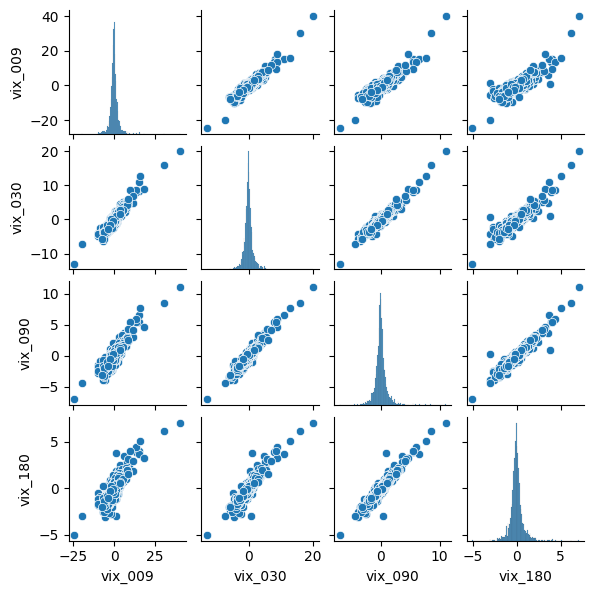
\includegraphics{chapters/12_seaborn/seaborn_files/figure-pdf/cell-5-output-1.png}

}

\end{figure}

\hypertarget{graphing-with-seaborn}{%
\subsection{\texorpdfstring{Graphing with
\texttt{seaborn}}{Graphing with seaborn}}\label{graphing-with-seaborn}}

Let's create similar graphs with \textbf{seaborn}. Creating all four
plots in a single graph is not as easy with \textbf{seaborn} and the
code is a little confusing. To keep things simple we will recreate two
of the plots separately.

Here is the code that generates the graph of the daily prices.

\begin{Shaded}
\begin{Highlighting}[]
\ControlFlowTok{with}\NormalTok{ sns.axes\_style(}\StringTok{\textquotesingle{}darkgrid\textquotesingle{}}\NormalTok{):}
\NormalTok{    g }\OperatorTok{=}\NormalTok{ sns.relplot(x}\OperatorTok{=}\StringTok{\textquotesingle{}date\textquotesingle{}}\NormalTok{, y}\OperatorTok{=}\StringTok{\textquotesingle{}spy\textquotesingle{}}\NormalTok{, kind}\OperatorTok{=}\StringTok{\textquotesingle{}line\textquotesingle{}}\NormalTok{, data}\OperatorTok{=}\NormalTok{df\_spy, aspect}\OperatorTok{=}\FloatTok{1.5}\NormalTok{)}
\NormalTok{    g.fig.autofmt\_xdate()}
    \CommentTok{\# creating and tweaking the title}
\NormalTok{    g.fig.suptitle(}\StringTok{\textquotesingle{}SPY Close Price: 2016Q1{-}2021Q2\textquotesingle{}}\NormalTok{)}
\NormalTok{    plt.subplots\_adjust(top}\OperatorTok{=}\FloatTok{0.93}\NormalTok{)}\OperatorTok{;}
\end{Highlighting}
\end{Shaded}

\begin{figure}[H]

{\centering 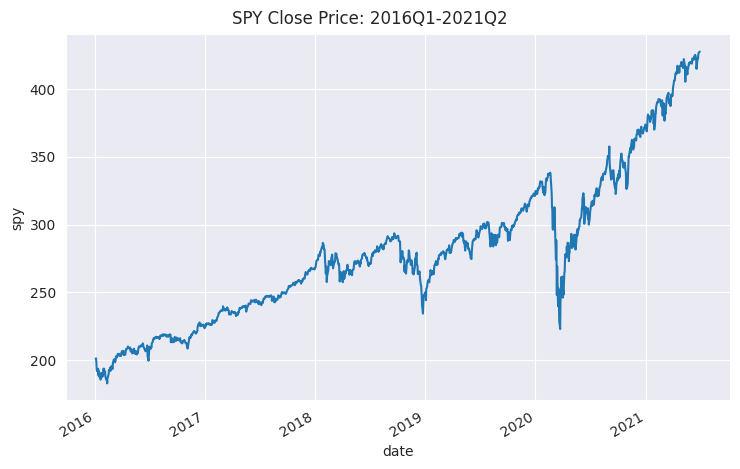
\includegraphics{chapters/12_seaborn/seaborn_files/figure-pdf/cell-6-output-1.png}

}

\end{figure}

And here is the code produces the graph of the daily returns.

\begin{Shaded}
\begin{Highlighting}[]
\ControlFlowTok{with}\NormalTok{ sns.axes\_style(}\StringTok{\textquotesingle{}darkgrid\textquotesingle{}}\NormalTok{):}
\NormalTok{    g }\OperatorTok{=}\NormalTok{ sns.relplot(x}\OperatorTok{=}\StringTok{\textquotesingle{}date\textquotesingle{}}\NormalTok{, y}\OperatorTok{=}\StringTok{\textquotesingle{}return\textquotesingle{}}\NormalTok{, kind}\OperatorTok{=}\StringTok{\textquotesingle{}line\textquotesingle{}}\NormalTok{, data}\OperatorTok{=}\NormalTok{df\_spy, aspect}\OperatorTok{=}\FloatTok{1.5}\NormalTok{)}
\NormalTok{    g.fig.autofmt\_xdate()}
    \CommentTok{\# creating and tweaking the title}
\NormalTok{    g.fig.suptitle(}\StringTok{\textquotesingle{}SPY Close Price: 2016Q1{-}2021Q2\textquotesingle{}}\NormalTok{)}\OperatorTok{;}
\NormalTok{    plt.subplots\_adjust(top}\OperatorTok{=}\FloatTok{0.93}\NormalTok{)}\OperatorTok{;}
\end{Highlighting}
\end{Shaded}

\begin{figure}[H]

{\centering \includegraphics{chapters/12_seaborn/seaborn_files/figure-pdf/cell-7-output-1.png}

}

\end{figure}

\hypertarget{bar-graph---monthly-spy-call-pnls}{%
\section{Bar Graph - Monthly SPY Call
PNLs}\label{bar-graph---monthly-spy-call-pnls}}

Our next data set consists of monthly pnls from the call trades detailed
in \texttt{seaborn\_monthly\_pnl\_bar.csv}.

\begin{Shaded}
\begin{Highlighting}[]
\NormalTok{df\_monthly\_bar }\OperatorTok{=}\NormalTok{ pd.read\_csv(}\StringTok{\textquotesingle{}seaborn\_monthly\_pnl\_bar.csv\textquotesingle{}}\NormalTok{)}
\NormalTok{df\_monthly\_bar.head()}
\end{Highlighting}
\end{Shaded}

\begin{longtable}[]{@{}llll@{}}
\toprule\noalign{}
& month & year & monthly\_pnl \\
\midrule\noalign{}
\endhead
\bottomrule\noalign{}
\endlastfoot
0 & 1 & 2018 & 0.091963 \\
1 & 2 & 2018 & -2.759090 \\
2 & 3 & 2018 & -0.340270 \\
3 & 4 & 2018 & -1.174222 \\
4 & 5 & 2018 & 1.487206 \\
\end{longtable}

\hypertarget{graphing-with-pandas-1}{%
\subsection{\texorpdfstring{Graphing with
\texttt{pandas}}{Graphing with pandas}}\label{graphing-with-pandas-1}}

Recall that this code creates the barplot of the pnls by month using
\textbf{pandas}.

\begin{Shaded}
\begin{Highlighting}[]
\NormalTok{ax }\OperatorTok{=} \OperatorTok{\textbackslash{}}
\NormalTok{    (df\_monthly\_bar}
\NormalTok{        .plot(}
\NormalTok{            x }\OperatorTok{=} \StringTok{\textquotesingle{}month\textquotesingle{}}\NormalTok{,}
\NormalTok{            y }\OperatorTok{=}\NormalTok{ [}\StringTok{\textquotesingle{}monthly\_pnl\textquotesingle{}}\NormalTok{],}
\NormalTok{            kind }\OperatorTok{=}\StringTok{\textquotesingle{}bar\textquotesingle{}}\NormalTok{,}
\NormalTok{            color}\OperatorTok{=}\StringTok{\textquotesingle{}k\textquotesingle{}}\NormalTok{, }\CommentTok{\# color is grey}
\NormalTok{            grid}\OperatorTok{=}\VariableTok{True}\NormalTok{, }\CommentTok{\# adding a grid}
\NormalTok{            alpha}\OperatorTok{=}\FloatTok{0.75}\NormalTok{, }\CommentTok{\# translucence}
\NormalTok{            width}\OperatorTok{=}\FloatTok{0.8}\NormalTok{, }\CommentTok{\# increasing the width of the bars}
\NormalTok{            title}\OperatorTok{=}\StringTok{\textquotesingle{}Monthly PNL for SPY Calls\textquotesingle{}}\NormalTok{,}
\NormalTok{            figsize}\OperatorTok{=}\NormalTok{(}\DecValTok{8}\NormalTok{, }\DecValTok{5}\NormalTok{), }\CommentTok{\# modifying the figure size}
\NormalTok{        ))}\OperatorTok{;}

\NormalTok{ax.set\_xlabel(}\StringTok{"Month"}\NormalTok{)}\OperatorTok{;} \CommentTok{\# x{-}axis label}
\NormalTok{ax.set\_ylabel(}\StringTok{"PNL"}\NormalTok{)}\OperatorTok{;}   \CommentTok{\# y{-}axis label}
\end{Highlighting}
\end{Shaded}

\begin{figure}[H]

{\centering \includegraphics{chapters/12_seaborn/seaborn_files/figure-pdf/cell-9-output-1.png}

}

\end{figure}

\hypertarget{graphing-with-seaborn-1}{%
\subsection{\texorpdfstring{Graphing with
\texttt{seaborn}}{Graphing with seaborn}}\label{graphing-with-seaborn-1}}

Here is the code that produces a similar graph in using
\textbf{seaborn}.

\begin{Shaded}
\begin{Highlighting}[]
\ControlFlowTok{with}\NormalTok{ sns.axes\_style(}\StringTok{\textquotesingle{}darkgrid\textquotesingle{}}\NormalTok{):}
\NormalTok{    g }\OperatorTok{=}\NormalTok{ sns.catplot(}
\NormalTok{        x}\OperatorTok{=}\StringTok{\textquotesingle{}month\textquotesingle{}}
\NormalTok{        , y}\OperatorTok{=}\StringTok{\textquotesingle{}monthly\_pnl\textquotesingle{}}
\NormalTok{        , kind}\OperatorTok{=}\StringTok{\textquotesingle{}bar\textquotesingle{}}
\NormalTok{        , color}\OperatorTok{=}\StringTok{\textquotesingle{}black\textquotesingle{}}
\NormalTok{        , alpha}\OperatorTok{=}\FloatTok{0.75}
\NormalTok{        , height}\OperatorTok{=}\DecValTok{5}
\NormalTok{        , aspect }\OperatorTok{=} \FloatTok{1.5}
\NormalTok{        , data}\OperatorTok{=}\NormalTok{df\_monthly\_bar}
\NormalTok{    )}\OperatorTok{;}
\NormalTok{    plt.subplots\_adjust(top}\OperatorTok{=}\FloatTok{0.93}\NormalTok{)}\OperatorTok{;}
\NormalTok{    g.fig.suptitle(}\StringTok{\textquotesingle{}Monthly PNL for SPY Calls\textquotesingle{}}\NormalTok{)}\OperatorTok{;}
\end{Highlighting}
\end{Shaded}

\begin{figure}[H]

{\centering \includegraphics{chapters/12_seaborn/seaborn_files/figure-pdf/cell-10-output-1.png}

}

\end{figure}

\hypertarget{scatter-plot---spy-returns-vs-vix-change-implied-leverage}{%
\section{\texorpdfstring{Scatter Plot - SPY Returns vs VIX Change
(\emph{implied
leverage})}{Scatter Plot - SPY Returns vs VIX Change (implied leverage)}}\label{scatter-plot---spy-returns-vs-vix-change-implied-leverage}}

Let's add \texttt{vix\_chng} to \texttt{df\_spy} and change the units to
decimals.

\begin{Shaded}
\begin{Highlighting}[]
\NormalTok{df\_spy[}\StringTok{\textquotesingle{}vix\_chng\textquotesingle{}}\NormalTok{] }\OperatorTok{=}\NormalTok{ df\_spy[}\StringTok{\textquotesingle{}vix\textquotesingle{}}\NormalTok{].diff()}
\NormalTok{df\_spy[}\StringTok{\textquotesingle{}vix\textquotesingle{}}\NormalTok{] }\OperatorTok{=}\NormalTok{ df\_spy[}\StringTok{\textquotesingle{}vix\textquotesingle{}}\NormalTok{] }\OperatorTok{/} \DecValTok{100}
\NormalTok{df\_spy[}\StringTok{\textquotesingle{}vix\_chng\textquotesingle{}}\NormalTok{] }\OperatorTok{=}\NormalTok{ df\_spy[}\StringTok{\textquotesingle{}vix\_chng\textquotesingle{}}\NormalTok{] }\OperatorTok{/} \DecValTok{100}
\NormalTok{df\_spy.head()}
\end{Highlighting}
\end{Shaded}

\begin{longtable}[]{@{}lllllll@{}}
\toprule\noalign{}
& date & spy & vix & return & realized\_vol & vix\_chng \\
\midrule\noalign{}
\endhead
\bottomrule\noalign{}
\endlastfoot
0 & 2016-01-04 & 201.02 & 0.2070 & NaN & NaN & NaN \\
1 & 2016-01-05 & 201.36 & 0.1934 & 0.001691 & NaN & -0.0136 \\
2 & 2016-01-06 & 198.82 & 0.2059 & -0.012614 & NaN & 0.0125 \\
3 & 2016-01-07 & 194.05 & 0.2499 & -0.023992 & NaN & 0.0440 \\
4 & 2016-01-08 & 191.92 & 0.2701 & -0.010977 & NaN & 0.0202 \\
\end{longtable}

\hypertarget{graphing-with-pandas-2}{%
\subsection{\texorpdfstring{Graphing with
\texttt{pandas}}{Graphing with pandas}}\label{graphing-with-pandas-2}}

Here is the \textbf{pandas} code that creates scatter plot of returns vs
VIX changes.

\begin{Shaded}
\begin{Highlighting}[]
\NormalTok{df\_spy.plot.scatter(}
\NormalTok{    x }\OperatorTok{=} \StringTok{\textquotesingle{}return\textquotesingle{}}\NormalTok{,}
\NormalTok{    y }\OperatorTok{=} \StringTok{\textquotesingle{}vix\_chng\textquotesingle{}}\NormalTok{,}
\NormalTok{    grid}\OperatorTok{=}\VariableTok{True}\NormalTok{ ,  }
\NormalTok{    c}\OperatorTok{=}\StringTok{\textquotesingle{}k\textquotesingle{}}\NormalTok{,}
\NormalTok{    alpha}\OperatorTok{=}\FloatTok{0.75}\NormalTok{,}
\NormalTok{    s}\OperatorTok{=}\DecValTok{10}\NormalTok{, }\CommentTok{\# changing the size of the dots}
\NormalTok{    figsize}\OperatorTok{=}\NormalTok{(}\DecValTok{7}\NormalTok{, }\DecValTok{5}\NormalTok{),}
\NormalTok{    title}\OperatorTok{=}\StringTok{\textquotesingle{}SPY Return vs VIX Changes: 2016Q1{-}2021Q2\textquotesingle{}}\NormalTok{,}
\NormalTok{)}\OperatorTok{;}
\end{Highlighting}
\end{Shaded}

\begin{figure}[H]

{\centering \includegraphics{chapters/12_seaborn/seaborn_files/figure-pdf/cell-12-output-1.png}

}

\end{figure}

\hypertarget{graphing-with-seaborn-2}{%
\subsection{\texorpdfstring{Graphing with
\texttt{seaborn}}{Graphing with seaborn}}\label{graphing-with-seaborn-2}}

Here is the code for a similar graph using \textbf{seaborn}.

\begin{Shaded}
\begin{Highlighting}[]
\ControlFlowTok{with}\NormalTok{ sns.axes\_style(}\StringTok{\textquotesingle{}darkgrid\textquotesingle{}}\NormalTok{):}
\NormalTok{    g }\OperatorTok{=}\NormalTok{ sns.relplot(}
\NormalTok{            x }\OperatorTok{=} \StringTok{\textquotesingle{}return\textquotesingle{}}\NormalTok{,}
\NormalTok{            y }\OperatorTok{=} \StringTok{\textquotesingle{}vix\_chng\textquotesingle{}}\NormalTok{,}
\NormalTok{            data }\OperatorTok{=}\NormalTok{ df\_spy,}
\NormalTok{            color }\OperatorTok{=} \StringTok{\textquotesingle{}black\textquotesingle{}}\NormalTok{,}
\NormalTok{            alpha }\OperatorTok{=} \FloatTok{0.75}\NormalTok{,}
\NormalTok{            height }\OperatorTok{=} \FloatTok{5.5}\NormalTok{,}
\NormalTok{            aspect }\OperatorTok{=} \FloatTok{1.3}\NormalTok{,}
\NormalTok{        )}\OperatorTok{;}
\NormalTok{    plt.subplots\_adjust(top}\OperatorTok{=}\FloatTok{0.93}\NormalTok{)}\OperatorTok{;}
\NormalTok{    g.fig.suptitle(}\StringTok{\textquotesingle{}SPY Return vs VIX Changes: 2016Q1{-}2021Q2)\textquotesingle{}}\NormalTok{)}\OperatorTok{;}
\end{Highlighting}
\end{Shaded}

\begin{figure}[H]

{\centering \includegraphics{chapters/12_seaborn/seaborn_files/figure-pdf/cell-13-output-1.png}

}

\end{figure}

\hypertarget{further-reading-2}{%
\section{Further Reading}\label{further-reading-2}}

\emph{Python Data Science Handbook} - 4.14 - Visualization with Seaborn

Seaborn Official Tutorials - https://seaborn.pydata.org/tutorial.html
(very good, but long)

\hypertarget{basic-plotting-with-bokeh}{%
\chapter{\texorpdfstring{Basic Plotting with
\textbf{bokeh}}{Basic Plotting with bokeh}}\label{basic-plotting-with-bokeh}}

In this notebook we create some basic interactive plots with the
\textbf{bokeh} package. These plots come with a fair amount of
interactivity out of the box. In a subsequent chapter we will add more
advanced interactivity.

\hypertarget{data}{%
\section{Data}\label{data}}

Let's begin by loading the data that we will need for our
visualizations.

\begin{Shaded}
\begin{Highlighting}[]
\ImportTok{import}\NormalTok{ numpy }\ImportTok{as}\NormalTok{ np}
\ImportTok{import}\NormalTok{ pandas }\ImportTok{as}\NormalTok{ pd}
\ImportTok{import}\NormalTok{ yfinance }\ImportTok{as}\NormalTok{ yf}
\NormalTok{yf.pdr\_override()}
\ImportTok{from}\NormalTok{ pandas\_datareader }\ImportTok{import}\NormalTok{ data }\ImportTok{as}\NormalTok{ pdr}

\CommentTok{\# SPY Close, Returns, Realized Volatility, and VIX}
\NormalTok{df\_spy }\OperatorTok{=}\NormalTok{ pdr.get\_data\_yahoo([}\StringTok{\textquotesingle{}SPY\textquotesingle{}}\NormalTok{, }\StringTok{\textquotesingle{}\^{}VIX\textquotesingle{}}\NormalTok{], start}\OperatorTok{=}\StringTok{\textquotesingle{}2016{-}01{-}01\textquotesingle{}}\NormalTok{, end}\OperatorTok{=}\StringTok{\textquotesingle{}2021{-}09{-}30\textquotesingle{}}\NormalTok{)}
\NormalTok{df\_spy }\OperatorTok{=}\NormalTok{ df\_spy.}\BuiltInTok{round}\NormalTok{(}\DecValTok{2}\NormalTok{)}
\NormalTok{df\_spy }\OperatorTok{=}\NormalTok{ df\_spy[}\StringTok{\textquotesingle{}Close\textquotesingle{}}\NormalTok{].reset\_index()}
\NormalTok{df\_spy.rename(columns}\OperatorTok{=}\NormalTok{\{}\StringTok{\textquotesingle{}Date\textquotesingle{}}\NormalTok{:}\StringTok{\textquotesingle{}date\textquotesingle{}}\NormalTok{,}\StringTok{\textquotesingle{}SPY\textquotesingle{}}\NormalTok{:}\StringTok{\textquotesingle{}close\textquotesingle{}}\NormalTok{,}\StringTok{\textquotesingle{}\^{}VIX\textquotesingle{}}\NormalTok{:}\StringTok{\textquotesingle{}vix\textquotesingle{}}\NormalTok{\}, inplace}\OperatorTok{=}\VariableTok{True}\NormalTok{)}
\NormalTok{df\_spy[}\StringTok{\textquotesingle{}return\textquotesingle{}}\NormalTok{] }\OperatorTok{=}\NormalTok{ np.log(df\_spy[}\StringTok{\textquotesingle{}close\textquotesingle{}}\NormalTok{] }\OperatorTok{/}\NormalTok{ df\_spy[}\StringTok{\textquotesingle{}close\textquotesingle{}}\NormalTok{].shift(}\DecValTok{1}\NormalTok{))}
\NormalTok{df\_spy[}\StringTok{\textquotesingle{}realized\_vol\textquotesingle{}}\NormalTok{] }\OperatorTok{=}\NormalTok{ df\_spy[}\StringTok{\textquotesingle{}return\textquotesingle{}}\NormalTok{].rolling(}\DecValTok{42}\NormalTok{).std() }\OperatorTok{*}\NormalTok{ np.sqrt(}\DecValTok{252}\NormalTok{)}

\CommentTok{\# SPY Monthly Returns}
\NormalTok{df\_spy[}\StringTok{\textquotesingle{}year\textquotesingle{}}\NormalTok{] }\OperatorTok{=}\NormalTok{ df\_spy[}\StringTok{\textquotesingle{}date\textquotesingle{}}\NormalTok{].dt.year}
\NormalTok{df\_spy[}\StringTok{\textquotesingle{}month\textquotesingle{}}\NormalTok{] }\OperatorTok{=}\NormalTok{ df\_spy[}\StringTok{\textquotesingle{}date\textquotesingle{}}\NormalTok{].dt.month}
\NormalTok{df\_monthly }\OperatorTok{=}\NormalTok{ df\_spy.groupby([}\StringTok{\textquotesingle{}year\textquotesingle{}}\NormalTok{, }\StringTok{\textquotesingle{}month\textquotesingle{}}\NormalTok{], as\_index}\OperatorTok{=}\VariableTok{False}\NormalTok{)[[}\StringTok{\textquotesingle{}return\textquotesingle{}}\NormalTok{]].}\BuiltInTok{sum}\NormalTok{()}
\NormalTok{df\_monthly[}\StringTok{\textquotesingle{}year\_month\textquotesingle{}}\NormalTok{] }\OperatorTok{=}\NormalTok{ (df\_monthly[}\StringTok{\textquotesingle{}year\textquotesingle{}}\NormalTok{] }\OperatorTok{*} \DecValTok{100}\NormalTok{) }\OperatorTok{+}\NormalTok{ df\_monthly[}\StringTok{\textquotesingle{}month\textquotesingle{}}\NormalTok{]}
\NormalTok{df\_monthly[}\StringTok{\textquotesingle{}year\_month\textquotesingle{}}\NormalTok{] }\OperatorTok{=}\NormalTok{ df\_monthly[}\StringTok{\textquotesingle{}year\_month\textquotesingle{}}\NormalTok{].astype(}\BuiltInTok{str}\NormalTok{)}

\CommentTok{\# Implied Leverage Effect}
\NormalTok{df\_spy[}\StringTok{\textquotesingle{}vix\_change\textquotesingle{}}\NormalTok{] }\OperatorTok{=}\NormalTok{ df\_spy[}\StringTok{\textquotesingle{}vix\textquotesingle{}}\NormalTok{].diff()}
\NormalTok{df\_spy[}\StringTok{\textquotesingle{}vix\textquotesingle{}}\NormalTok{] }\OperatorTok{=}\NormalTok{ df\_spy[}\StringTok{\textquotesingle{}vix\textquotesingle{}}\NormalTok{] }\OperatorTok{/} \DecValTok{100}
\NormalTok{df\_spy[}\StringTok{\textquotesingle{}vix\_change\textquotesingle{}}\NormalTok{] }\OperatorTok{=}\NormalTok{ df\_spy[}\StringTok{\textquotesingle{}vix\_change\textquotesingle{}}\NormalTok{] }\OperatorTok{/} \DecValTok{100}

\CommentTok{\# Asset Allocation {-} hypothetical allocation through time}
\NormalTok{df\_asset\_allocation }\OperatorTok{=}\NormalTok{ pd.read\_csv(}\StringTok{\textquotesingle{}asset\_allocation.csv\textquotesingle{}}\NormalTok{, parse\_dates}\OperatorTok{=}\NormalTok{[}\StringTok{\textquotesingle{}trade\_date\textquotesingle{}}\NormalTok{])}
\end{Highlighting}
\end{Shaded}

\begin{verbatim}
[*********************100%***********************]  2 of 2 completed
\end{verbatim}

\hypertarget{two-interfaces}{%
\section{Two Interfaces}\label{two-interfaces}}

There are two interfaces for working with \textbf{bokeh}:

\texttt{bokeh.models}: a low level interface that gives you complete
control over how \textbf{bokeh} creates all elements of your
visualization.

\texttt{bokeh.plotting}: a high level, general-purpose interface that is
similar to plotting interfaces of libraries such as Matplotlib or
Matlab. It automatically assembles plots with default elements such as
axes, grids, and tools for you.

Our focus will be on the \texttt{bokeh.plotting} interface.

\hypertarget{blank-graph}{%
\section{Blank Graph}\label{blank-graph}}

Let's begin by creating a blank graph, and examine the elements of the
code:

\texttt{bokeh.io.output\_notebook()} - output the graph inline in the
notebook.

\texttt{bokeh.plotting.figure()} - creates the basic plot object, called
a \texttt{Figure} model.

\texttt{bokeh.plotting.show()} - outputs the \texttt{Figure} model.

\begin{Shaded}
\begin{Highlighting}[]
\CommentTok{\# import bokeh functions}
\ImportTok{from}\NormalTok{ bokeh.io }\ImportTok{import}\NormalTok{ output\_notebook}
\ImportTok{from}\NormalTok{ bokeh.plotting }\ImportTok{import}\NormalTok{ figure, show}

\CommentTok{\# output inline}
\NormalTok{output\_notebook()}

\CommentTok{\# create figure() object with a title}
\NormalTok{fig }\OperatorTok{=}\NormalTok{ figure(title}\OperatorTok{=}\StringTok{\textquotesingle{}Blank Figure\textquotesingle{}}\NormalTok{)}

\CommentTok{\# output to notebook}
\NormalTok{show(fig)}
\end{Highlighting}
\end{Shaded}

\begin{verbatim}
Unable to display output for mime type(s): text/html
\end{verbatim}

\begin{verbatim}
Unable to display output for mime type(s): application/javascript, application/vnd.bokehjs_load.v0+json
\end{verbatim}

\begin{verbatim}
WARNING:bokeh.core.validation.check:W-1000 (MISSING_RENDERERS): Plot has no renderers: figure(id='p1001', ...)
\end{verbatim}

\begin{verbatim}
Unable to display output for mime type(s): text/html
\end{verbatim}

\begin{verbatim}
Unable to display output for mime type(s): application/javascript, application/vnd.bokehjs_exec.v0+json
\end{verbatim}

Notice the toolbar on the right of the figure above which has a variety
of interactive tools. These aren't that interesting at the moment
because our graph is blank.

\hypertarget{basic-line-plot}{%
\section{Basic Line Plot}\label{basic-line-plot}}

Let's create our first proper graph by adding a \texttt{line} glyph that
plots the SPY close prices.

Notice that we also modify our \texttt{Figure} object by adding
arguments to the \texttt{figure()} function.

Now the interactive tools are a bit more interesting.

\begin{Shaded}
\begin{Highlighting}[]
\CommentTok{\# import bokeh functions}
\ImportTok{from}\NormalTok{ bokeh.io }\ImportTok{import}\NormalTok{ output\_notebook, show}
\ImportTok{from}\NormalTok{ bokeh.plotting }\ImportTok{import}\NormalTok{ figure}

\CommentTok{\# output inline}
\NormalTok{output\_notebook()}

\CommentTok{\# create figure() object with a title}
\NormalTok{p }\OperatorTok{=}\NormalTok{ figure(width}\OperatorTok{=}\DecValTok{600}\NormalTok{, height}\OperatorTok{=}\DecValTok{400}\NormalTok{, x\_axis\_type}\OperatorTok{=}\StringTok{\textquotesingle{}datetime\textquotesingle{}}\NormalTok{, title}\OperatorTok{=}\StringTok{\textquotesingle{}SPY Close Price\textquotesingle{}}\NormalTok{,}
\NormalTok{           x\_axis\_label}\OperatorTok{=}\StringTok{\textquotesingle{}date\textquotesingle{}}\NormalTok{, y\_axis\_label}\OperatorTok{=}\StringTok{\textquotesingle{}close price\textquotesingle{}}\NormalTok{)}

\CommentTok{\# adding a line glyph to display close prices by passing data Series directly}
\NormalTok{p.line(x}\OperatorTok{=}\NormalTok{df\_spy[}\StringTok{\textquotesingle{}date\textquotesingle{}}\NormalTok{], y}\OperatorTok{=}\NormalTok{df\_spy[}\StringTok{\textquotesingle{}close\textquotesingle{}}\NormalTok{])}

\CommentTok{\# output to notebook}
\NormalTok{show(p)}
\end{Highlighting}
\end{Shaded}

\begin{verbatim}
Unable to display output for mime type(s): text/html
\end{verbatim}

\begin{verbatim}
Unable to display output for mime type(s): application/javascript, application/vnd.bokehjs_load.v0+json
\end{verbatim}

\begin{verbatim}
Unable to display output for mime type(s): text/html
\end{verbatim}

\begin{verbatim}
Unable to display output for mime type(s): application/javascript, application/vnd.bokehjs_exec.v0+json
\end{verbatim}

\hypertarget{columndatasource}{%
\section{\texorpdfstring{\texttt{ColumnDataSource}}{ColumnDataSource}}\label{columndatasource}}

In the example above, we passed our data to be graphed directly into the
\texttt{p.line()} glyph by specifying particular columns of
\texttt{df\_spy}, which is a \texttt{pandas.DataFrame}. If you recall,
the columns of a \texttt{DataFrame} are \texttt{pandas.Series} objects.
We can also pass \texttt{lists} and \texttt{numpy.arrays} directly into
a glyph.

However, it is more fruitful to use a \texttt{ColumnDataSource} object.
We can easily create one from a \texttt{DataFrame} called \texttt{df}
with the following syntax: \texttt{ColumnDataSource(df)}.

\begin{Shaded}
\begin{Highlighting}[]
\CommentTok{\# import bokeh functions}
\ImportTok{from}\NormalTok{ bokeh.io }\ImportTok{import}\NormalTok{ output\_notebook, show}
\ImportTok{from}\NormalTok{ bokeh.plotting }\ImportTok{import}\NormalTok{ figure}
\ImportTok{from}\NormalTok{ bokeh.models }\ImportTok{import}\NormalTok{ ColumnDataSource}

\CommentTok{\# output inline}
\NormalTok{output\_notebook()}

\CommentTok{\# creating ColumnDataSource from DataFrame}
\NormalTok{cds }\OperatorTok{=}\NormalTok{ ColumnDataSource(df\_spy)}

\CommentTok{\# creating figure() object}
\NormalTok{p }\OperatorTok{=}\NormalTok{ figure(width}\OperatorTok{=}\DecValTok{600}\NormalTok{, height}\OperatorTok{=}\DecValTok{400}\NormalTok{, x\_axis\_type}\OperatorTok{=}\StringTok{\textquotesingle{}datetime\textquotesingle{}}\NormalTok{, title}\OperatorTok{=}\StringTok{\textquotesingle{}SPY Close Price\textquotesingle{}}\NormalTok{,}
\NormalTok{           x\_axis\_label}\OperatorTok{=}\StringTok{\textquotesingle{}date\textquotesingle{}}\NormalTok{, y\_axis\_label}\OperatorTok{=}\StringTok{\textquotesingle{}close price\textquotesingle{}}\NormalTok{)}

\CommentTok{\# adding a line glyph to display close prices, passing data via ColumnDataSource}
\NormalTok{p.line(x}\OperatorTok{=}\StringTok{\textquotesingle{}date\textquotesingle{}}\NormalTok{, y}\OperatorTok{=}\StringTok{\textquotesingle{}close\textquotesingle{}}\NormalTok{,source}\OperatorTok{=}\NormalTok{cds)}

\CommentTok{\# output to notebook}
\NormalTok{show(p)}
\end{Highlighting}
\end{Shaded}

\begin{verbatim}
Unable to display output for mime type(s): text/html
\end{verbatim}

\begin{verbatim}
Unable to display output for mime type(s): application/javascript, application/vnd.bokehjs_load.v0+json
\end{verbatim}

\begin{verbatim}
Unable to display output for mime type(s): text/html
\end{verbatim}

\begin{verbatim}
Unable to display output for mime type(s): application/javascript, application/vnd.bokehjs_exec.v0+json
\end{verbatim}

\hypertarget{basic-scatter}{%
\section{Basic Scatter}\label{basic-scatter}}

Next, let's create a basic scatter plot using the \texttt{.circle()}
glyph. Notice that we have reformatted the x-axis and y-axis to be
expressed as percents.

\begin{Shaded}
\begin{Highlighting}[]
\CommentTok{\# import bokeh functions}
\ImportTok{from}\NormalTok{ bokeh.io }\ImportTok{import}\NormalTok{ output\_notebook, show}
\ImportTok{from}\NormalTok{ bokeh.plotting }\ImportTok{import}\NormalTok{ figure}
\ImportTok{from}\NormalTok{ bokeh.models }\ImportTok{import}\NormalTok{ ColumnDataSource}
\ImportTok{from}\NormalTok{ bokeh.models }\ImportTok{import}\NormalTok{ NumeralTickFormatter}

\CommentTok{\# output inline}
\NormalTok{output\_notebook()}

\CommentTok{\# creating a ColumnDataSource from DataFrame}
\NormalTok{cds }\OperatorTok{=}\NormalTok{ ColumnDataSource(df\_spy)}

\CommentTok{\# creating figure() object with a title}
\CommentTok{\# p = figure(plot\_width=500, plot\_height=500, title=\textquotesingle{}SPY Implied Leverage Effect\textquotesingle{},}
\CommentTok{\#            x\_axis\_label=\textquotesingle{}return\textquotesingle{}, y\_axis\_label=\textquotesingle{}vix change\textquotesingle{})}
\NormalTok{p }\OperatorTok{=}\NormalTok{ figure(width}\OperatorTok{=}\DecValTok{500}\NormalTok{, height}\OperatorTok{=}\DecValTok{500}\NormalTok{, title}\OperatorTok{=}\StringTok{\textquotesingle{}SPY Implied Leverage Effect\textquotesingle{}}\NormalTok{,}
\NormalTok{           x\_axis\_label}\OperatorTok{=}\StringTok{\textquotesingle{}return\textquotesingle{}}\NormalTok{, y\_axis\_label}\OperatorTok{=}\StringTok{\textquotesingle{}vix change\textquotesingle{}}\NormalTok{)}

\CommentTok{\# adding circle glyph, passing data via ColumnDataSource}
\NormalTok{p.circle(}\StringTok{\textquotesingle{}return\textquotesingle{}}\NormalTok{, }\StringTok{\textquotesingle{}vix\_change\textquotesingle{}}\NormalTok{, source}\OperatorTok{=}\NormalTok{cds)}

\CommentTok{\# formatting the x{-}axis and y{-}axis to percents}
\NormalTok{p.xaxis.formatter }\OperatorTok{=}\NormalTok{ NumeralTickFormatter(}\BuiltInTok{format}\OperatorTok{=}\StringTok{\textquotesingle{}0\%\textquotesingle{}}\NormalTok{) }
\NormalTok{p.yaxis.formatter }\OperatorTok{=}\NormalTok{ NumeralTickFormatter(}\BuiltInTok{format}\OperatorTok{=}\StringTok{\textquotesingle{}0\%\textquotesingle{}}\NormalTok{)}

\CommentTok{\# output to notebook           }
\NormalTok{show(p)}
\end{Highlighting}
\end{Shaded}

\begin{verbatim}
Unable to display output for mime type(s): text/html
\end{verbatim}

\begin{verbatim}
Unable to display output for mime type(s): application/javascript, application/vnd.bokehjs_load.v0+json
\end{verbatim}

\begin{verbatim}
Unable to display output for mime type(s): text/html
\end{verbatim}

\begin{verbatim}
Unable to display output for mime type(s): application/javascript, application/vnd.bokehjs_exec.v0+json
\end{verbatim}

\hypertarget{other-glyphs}{%
\section{Other Glyphs}\label{other-glyphs}}

We can recreate this scatter plot with a larger hexes instead of
circles. We also modified the outline color and fill color, both of
which were affected by arguments to \texttt{p.hex()}.

\begin{Shaded}
\begin{Highlighting}[]
\CommentTok{\# import bokeh functions}
\ImportTok{from}\NormalTok{ bokeh.io }\ImportTok{import}\NormalTok{ output\_notebook, show}
\ImportTok{from}\NormalTok{ bokeh.plotting }\ImportTok{import}\NormalTok{ figure}
\ImportTok{from}\NormalTok{ bokeh.models }\ImportTok{import}\NormalTok{ ColumnDataSource}

\CommentTok{\# outpute inline}
\NormalTok{output\_notebook()}

\CommentTok{\# creating ColumnDataSource from DataFrame}
\NormalTok{cds }\OperatorTok{=}\NormalTok{ ColumnDataSource(df\_spy)}

\CommentTok{\# creating figure() object}
\NormalTok{p }\OperatorTok{=}\NormalTok{ figure(width}\OperatorTok{=}\DecValTok{600}\NormalTok{, height}\OperatorTok{=}\DecValTok{400}\NormalTok{, title}\OperatorTok{=}\StringTok{\textquotesingle{}SPY Implied Leverage Effect\textquotesingle{}}\NormalTok{,}
\NormalTok{           x\_axis\_label}\OperatorTok{=}\StringTok{\textquotesingle{}return\textquotesingle{}}\NormalTok{, y\_axis\_label}\OperatorTok{=}\StringTok{\textquotesingle{}vix change\textquotesingle{}}\NormalTok{)}

\CommentTok{\# adding hex glyph, while changing some visual paramenters}
\NormalTok{p.}\BuiltInTok{hex}\NormalTok{(}\StringTok{\textquotesingle{}return\textquotesingle{}}\NormalTok{, }\StringTok{\textquotesingle{}vix\_change\textquotesingle{}}\NormalTok{, line\_color}\OperatorTok{=}\StringTok{"navy"}\NormalTok{, fill\_color}\OperatorTok{=}\StringTok{"orange"}\NormalTok{, size}\OperatorTok{=}\DecValTok{15}\NormalTok{, source}\OperatorTok{=}\NormalTok{cds)}

\CommentTok{\# formatting the x{-}axis and y{-}axis to percents}
\NormalTok{p.xaxis.formatter }\OperatorTok{=}\NormalTok{ NumeralTickFormatter(}\BuiltInTok{format}\OperatorTok{=}\StringTok{\textquotesingle{}0\%\textquotesingle{}}\NormalTok{) }
\NormalTok{p.yaxis.formatter }\OperatorTok{=}\NormalTok{ NumeralTickFormatter(}\BuiltInTok{format}\OperatorTok{=}\StringTok{\textquotesingle{}0\%\textquotesingle{}}\NormalTok{)}

\NormalTok{show(p)}
\end{Highlighting}
\end{Shaded}

\begin{verbatim}
Unable to display output for mime type(s): text/html
\end{verbatim}

\begin{verbatim}
Unable to display output for mime type(s): application/javascript, application/vnd.bokehjs_load.v0+json
\end{verbatim}

\begin{verbatim}
Unable to display output for mime type(s): text/html
\end{verbatim}

\begin{verbatim}
Unable to display output for mime type(s): application/javascript, application/vnd.bokehjs_exec.v0+json
\end{verbatim}

\hypertarget{glyphs-gallery}{%
\subsection{Glyphs Gallery}\label{glyphs-gallery}}

There are a wide variety of glyphs that can be used for scatter plots.
They are demonstrated below in a visual that I borrowed from the
\textbf{bokeh} documentation.

\begin{Shaded}
\begin{Highlighting}[]
\ImportTok{from}\NormalTok{ numpy.random }\ImportTok{import}\NormalTok{ random}
\ImportTok{from}\NormalTok{ bokeh.io }\ImportTok{import}\NormalTok{ output\_notebook}
\ImportTok{from}\NormalTok{ bokeh.core.enums }\ImportTok{import}\NormalTok{ MarkerType}
\ImportTok{from}\NormalTok{ bokeh.plotting }\ImportTok{import}\NormalTok{ figure, show}


\NormalTok{output\_notebook()}

\NormalTok{p }\OperatorTok{=}\NormalTok{ figure(title}\OperatorTok{=}\StringTok{"Bokeh Markers"}\NormalTok{, toolbar\_location}\OperatorTok{=}\VariableTok{None}\NormalTok{)}
\NormalTok{p.grid.grid\_line\_color }\OperatorTok{=} \VariableTok{None}
\NormalTok{p.background\_fill\_color }\OperatorTok{=} \StringTok{"\#eeeeee"}
\NormalTok{p.axis.visible }\OperatorTok{=} \VariableTok{False}
\NormalTok{p.y\_range.flipped }\OperatorTok{=} \VariableTok{True}

\NormalTok{N }\OperatorTok{=} \DecValTok{10}

\ControlFlowTok{for}\NormalTok{ i, marker }\KeywordTok{in} \BuiltInTok{enumerate}\NormalTok{(MarkerType):}
\NormalTok{    x }\OperatorTok{=}\NormalTok{ i }\OperatorTok{\%} \DecValTok{4}
\NormalTok{    y }\OperatorTok{=}\NormalTok{ (i }\OperatorTok{//} \DecValTok{4}\NormalTok{) }\OperatorTok{*} \DecValTok{4} \OperatorTok{+} \DecValTok{1}

\NormalTok{    p.scatter(random(N)}\OperatorTok{+}\DecValTok{2}\OperatorTok{*}\NormalTok{x, random(N)}\OperatorTok{+}\NormalTok{y, marker}\OperatorTok{=}\NormalTok{marker, size}\OperatorTok{=}\DecValTok{14}\NormalTok{,}
\NormalTok{              line\_color}\OperatorTok{=}\StringTok{"navy"}\NormalTok{, fill\_color}\OperatorTok{=}\StringTok{"orange"}\NormalTok{, alpha}\OperatorTok{=}\FloatTok{0.5}\NormalTok{)}

\NormalTok{    p.text(}\DecValTok{2}\OperatorTok{*}\NormalTok{x}\OperatorTok{+}\FloatTok{0.5}\NormalTok{, y}\OperatorTok{+}\FloatTok{2.5}\NormalTok{, text}\OperatorTok{=}\NormalTok{[marker],}
\NormalTok{           text\_color}\OperatorTok{=}\StringTok{"firebrick"}\NormalTok{, text\_align}\OperatorTok{=}\StringTok{"center"}\NormalTok{, text\_font\_size}\OperatorTok{=}\StringTok{"13px"}\NormalTok{)}

\NormalTok{show(p)}
\end{Highlighting}
\end{Shaded}

\begin{verbatim}
Unable to display output for mime type(s): text/html
\end{verbatim}

\begin{verbatim}
Unable to display output for mime type(s): application/javascript, application/vnd.bokehjs_load.v0+json
\end{verbatim}

\begin{verbatim}
Unable to display output for mime type(s): text/html
\end{verbatim}

\begin{verbatim}
Unable to display output for mime type(s): application/javascript, application/vnd.bokehjs_exec.v0+json
\end{verbatim}

\hypertarget{barchart-with-monthly-returns}{%
\section{Barchart with Monthly
Returns}\label{barchart-with-monthly-returns}}

Here is a barchart of SPY monthly returns using the \texttt{p.vbar()}
renderer.

\begin{Shaded}
\begin{Highlighting}[]
\CommentTok{\# import bokeh functions}
\ImportTok{from}\NormalTok{ bokeh.io }\ImportTok{import}\NormalTok{ output\_notebook}
\ImportTok{from}\NormalTok{ bokeh.models }\ImportTok{import}\NormalTok{ ColumnDataSource}
\ImportTok{from}\NormalTok{ bokeh.models }\ImportTok{import}\NormalTok{ NumeralTickFormatter}
\ImportTok{from}\NormalTok{ bokeh.plotting }\ImportTok{import}\NormalTok{ figure, show}
\ImportTok{from}\NormalTok{ bokeh.plotting }\ImportTok{import}\NormalTok{ reset\_output}
\ImportTok{import}\NormalTok{ math}

\CommentTok{\# output inline}
\NormalTok{output\_notebook()}

\CommentTok{\# creating ColumnDataSource from DataFrame}
\NormalTok{source }\OperatorTok{=}\NormalTok{ ColumnDataSource(df\_monthly)}

\CommentTok{\# initializing the figure}
\NormalTok{p }\OperatorTok{=}\NormalTok{ figure(width}\OperatorTok{=}\DecValTok{1000}\NormalTok{, height}\OperatorTok{=}\DecValTok{400}\NormalTok{, x\_range}\OperatorTok{=}\NormalTok{df\_monthly[}\StringTok{\textquotesingle{}year\_month\textquotesingle{}}\NormalTok{], title}\OperatorTok{=}\StringTok{\textquotesingle{}SPY Monthly Returns 2016Q1 to 2021Q3\textquotesingle{}}\NormalTok{,}
\NormalTok{           x\_axis\_label}\OperatorTok{=}\StringTok{\textquotesingle{}month\textquotesingle{}}\NormalTok{, y\_axis\_label}\OperatorTok{=}\StringTok{\textquotesingle{}monthly return\textquotesingle{}}\NormalTok{)}

\CommentTok{\# adding vbar glyphs, passing data with ColumnDataSource}
\NormalTok{p.vbar(x}\OperatorTok{=}\StringTok{\textquotesingle{}year\_month\textquotesingle{}}\NormalTok{, bottom}\OperatorTok{=}\DecValTok{0}\NormalTok{, top}\OperatorTok{=}\StringTok{\textquotesingle{}return\textquotesingle{}}\NormalTok{, color}\OperatorTok{=}\StringTok{\textquotesingle{}blue\textquotesingle{}}\NormalTok{, width}\OperatorTok{=}\FloatTok{0.75}\NormalTok{, source}\OperatorTok{=}\NormalTok{source)}

\CommentTok{\# formatting the y{-}axis to percents}
\NormalTok{p.yaxis.formatter }\OperatorTok{=}\NormalTok{ NumeralTickFormatter(}\BuiltInTok{format}\OperatorTok{=}\StringTok{\textquotesingle{}0\%\textquotesingle{}}\NormalTok{)}

\CommentTok{\# rotating x{-}axis labels}
\NormalTok{p.xaxis.major\_label\_orientation }\OperatorTok{=}\NormalTok{ math.pi}\OperatorTok{/}\DecValTok{4}

\CommentTok{\# output graph}
\NormalTok{show(p)}
\end{Highlighting}
\end{Shaded}

\begin{verbatim}
Unable to display output for mime type(s): text/html
\end{verbatim}

\begin{verbatim}
Unable to display output for mime type(s): application/javascript, application/vnd.bokehjs_load.v0+json
\end{verbatim}

\begin{verbatim}
Unable to display output for mime type(s): text/html
\end{verbatim}

\begin{verbatim}
Unable to display output for mime type(s): application/javascript, application/vnd.bokehjs_exec.v0+json
\end{verbatim}

\hypertarget{stacked-areas-with-varying-asset-allocations}{%
\section{Stacked Areas with Varying Asset
Allocations}\label{stacked-areas-with-varying-asset-allocations}}

Next, we create a stacked area chart to visualize our hypotheticl asset
allocation that varies through time. In order to get a useful set of
colors, we need to use a palette from the \texttt{bokeh.palettes}
module.

\begin{Shaded}
\begin{Highlighting}[]
\CommentTok{\# import bokeh functions}
\ImportTok{import}\NormalTok{ bokeh}
\ImportTok{from}\NormalTok{ bokeh.models }\ImportTok{import}\NormalTok{ ColumnDataSource}
\ImportTok{from}\NormalTok{ bokeh.models }\ImportTok{import}\NormalTok{ NumeralTickFormatter}
\ImportTok{from}\NormalTok{ bokeh.plotting }\ImportTok{import}\NormalTok{ figure, output\_file, show}
\ImportTok{from}\NormalTok{ bokeh.io }\ImportTok{import}\NormalTok{ output\_notebook}
\ImportTok{import}\NormalTok{ pandas }\ImportTok{as}\NormalTok{ pd}

\CommentTok{\# output inline}
\NormalTok{output\_notebook()}

\CommentTok{\# putting data into ColumnDataSource object}
\NormalTok{source }\OperatorTok{=}\NormalTok{ ColumnDataSource(df\_asset\_allocation)}

\CommentTok{\# initializing the figure}
\NormalTok{p }\OperatorTok{=}\NormalTok{ figure(width}\OperatorTok{=}\DecValTok{900}\NormalTok{, height}\OperatorTok{=}\DecValTok{500}\NormalTok{, x\_axis\_type}\OperatorTok{=}\StringTok{\textquotesingle{}datetime\textquotesingle{}}\NormalTok{, title}\OperatorTok{=}\StringTok{\textquotesingle{}Asset Allocation 2019{-}2020\textquotesingle{}}\NormalTok{,}
\NormalTok{           x\_axis\_label}\OperatorTok{=}\StringTok{\textquotesingle{}month\textquotesingle{}}\NormalTok{, y\_axis\_label}\OperatorTok{=}\StringTok{\textquotesingle{}allocation\textquotesingle{}}\NormalTok{)}

\CommentTok{\# choosing assets and colors to graph}
\NormalTok{assets }\OperatorTok{=}\NormalTok{ df\_asset\_allocation.drop(columns}\OperatorTok{=}\StringTok{\textquotesingle{}trade\_date\textquotesingle{}}\NormalTok{).columns}
\NormalTok{num\_assets }\OperatorTok{=} \BuiltInTok{len}\NormalTok{(assets)}
\NormalTok{colors }\OperatorTok{=}\NormalTok{ bokeh.palettes.magma(num\_assets) }\CommentTok{\# choosing color palette}

\CommentTok{\# adding glyph with legend}
\NormalTok{p.varea\_stack(assets, x}\OperatorTok{=}\StringTok{\textquotesingle{}trade\_date\textquotesingle{}}\NormalTok{, color}\OperatorTok{=}\NormalTok{colors, source}\OperatorTok{=}\NormalTok{source, legend\_label}\OperatorTok{=}\NormalTok{assets.to\_list())}

\CommentTok{\# reversing order of legend to match order of graph}
\NormalTok{p.legend[}\DecValTok{0}\NormalTok{].items.reverse()}

\CommentTok{\# reformatting y{-}axis as percent }
\NormalTok{p.yaxis.formatter }\OperatorTok{=}\NormalTok{ NumeralTickFormatter(}\BuiltInTok{format}\OperatorTok{=}\StringTok{\textquotesingle{}0\%\textquotesingle{}}\NormalTok{)}

\CommentTok{\# moving legend off of the graph}
\NormalTok{p.add\_layout(p.legend[}\DecValTok{0}\NormalTok{], }\StringTok{\textquotesingle{}right\textquotesingle{}}\NormalTok{)}

\CommentTok{\# output graph}
\NormalTok{show(p)}
\end{Highlighting}
\end{Shaded}

\begin{verbatim}
Unable to display output for mime type(s): text/html
\end{verbatim}

\begin{verbatim}
Unable to display output for mime type(s): application/javascript, application/vnd.bokehjs_load.v0+json
\end{verbatim}

\begin{verbatim}
Unable to display output for mime type(s): text/html
\end{verbatim}

\begin{verbatim}
Unable to display output for mime type(s): application/javascript, application/vnd.bokehjs_exec.v0+json
\end{verbatim}

\hypertarget{layouts}{%
\section{Layouts}\label{layouts}}

Layout functions let you build a grid of plots and widgets. You can have
as many rows, columns, or grids of plots in one layout as you like.

We will use the \texttt{column()} function to vertically stack our
leverage effect line graphs. Notice that each graph has its own set of
interactive tools because they are not \emph{linked} together. We will
remedy this in the next notebook.

\begin{Shaded}
\begin{Highlighting}[]
\CommentTok{\# import bokeh functions}
\ImportTok{from}\NormalTok{ bokeh.io }\ImportTok{import}\NormalTok{ output\_notebook, show}
\ImportTok{from}\NormalTok{ bokeh.plotting }\ImportTok{import}\NormalTok{ figure}
\ImportTok{from}\NormalTok{ bokeh.layouts }\ImportTok{import}\NormalTok{ column}

\CommentTok{\# output inline}
\NormalTok{output\_notebook()}

\CommentTok{\# defining multiple plots}
\NormalTok{p1 }\OperatorTok{=}\NormalTok{ figure(width}\OperatorTok{=}\DecValTok{600}\NormalTok{, height}\OperatorTok{=}\DecValTok{200}\NormalTok{, x\_axis\_type}\OperatorTok{=}\StringTok{\textquotesingle{}datetime\textquotesingle{}}\NormalTok{, title}\OperatorTok{=}\StringTok{\textquotesingle{}SPY Leverage Effecct\textquotesingle{}}\NormalTok{)}
\NormalTok{p1.line(x}\OperatorTok{=}\NormalTok{df\_spy[}\StringTok{\textquotesingle{}date\textquotesingle{}}\NormalTok{], y}\OperatorTok{=}\NormalTok{df\_spy[}\StringTok{\textquotesingle{}close\textquotesingle{}}\NormalTok{])}

\NormalTok{p2 }\OperatorTok{=}\NormalTok{ figure(width}\OperatorTok{=}\DecValTok{600}\NormalTok{, height}\OperatorTok{=}\DecValTok{200}\NormalTok{, x\_axis\_type}\OperatorTok{=}\StringTok{\textquotesingle{}datetime\textquotesingle{}}\NormalTok{)}
\NormalTok{p2.line(x}\OperatorTok{=}\NormalTok{df\_spy[}\StringTok{\textquotesingle{}date\textquotesingle{}}\NormalTok{], y}\OperatorTok{=}\NormalTok{df\_spy[}\StringTok{\textquotesingle{}return\textquotesingle{}}\NormalTok{])}
\NormalTok{p2.yaxis.formatter }\OperatorTok{=}\NormalTok{ NumeralTickFormatter(}\BuiltInTok{format}\OperatorTok{=}\StringTok{\textquotesingle{}0\%\textquotesingle{}}\NormalTok{)}

\NormalTok{p3 }\OperatorTok{=}\NormalTok{ figure(width}\OperatorTok{=}\DecValTok{600}\NormalTok{, height}\OperatorTok{=}\DecValTok{200}\NormalTok{, x\_axis\_type}\OperatorTok{=}\StringTok{\textquotesingle{}datetime\textquotesingle{}}\NormalTok{)}
\NormalTok{p3.line(x}\OperatorTok{=}\NormalTok{df\_spy[}\StringTok{\textquotesingle{}date\textquotesingle{}}\NormalTok{], y}\OperatorTok{=}\NormalTok{df\_spy[}\StringTok{\textquotesingle{}realized\_vol\textquotesingle{}}\NormalTok{])}
\NormalTok{p3.yaxis.formatter }\OperatorTok{=}\NormalTok{ NumeralTickFormatter(}\BuiltInTok{format}\OperatorTok{=}\StringTok{\textquotesingle{}0\%\textquotesingle{}}\NormalTok{)}

\NormalTok{p4 }\OperatorTok{=}\NormalTok{ figure(width}\OperatorTok{=}\DecValTok{600}\NormalTok{, height}\OperatorTok{=}\DecValTok{200}\NormalTok{, x\_axis\_type}\OperatorTok{=}\StringTok{\textquotesingle{}datetime\textquotesingle{}}\NormalTok{)}
\NormalTok{p4.line(x}\OperatorTok{=}\NormalTok{df\_spy[}\StringTok{\textquotesingle{}date\textquotesingle{}}\NormalTok{], y}\OperatorTok{=}\NormalTok{df\_spy[}\StringTok{\textquotesingle{}vix\textquotesingle{}}\NormalTok{])}
\NormalTok{p4.yaxis.formatter }\OperatorTok{=}\NormalTok{ NumeralTickFormatter(}\BuiltInTok{format}\OperatorTok{=}\StringTok{\textquotesingle{}0\%\textquotesingle{}}\NormalTok{)}

\CommentTok{\# putting them together using column()}
\NormalTok{show(column(p1, p2, p3, p4))}
\end{Highlighting}
\end{Shaded}

\begin{verbatim}
Unable to display output for mime type(s): text/html
\end{verbatim}

\begin{verbatim}
Unable to display output for mime type(s): application/javascript, application/vnd.bokehjs_load.v0+json
\end{verbatim}

\begin{verbatim}
Unable to display output for mime type(s): text/html
\end{verbatim}

\begin{verbatim}
Unable to display output for mime type(s): application/javascript, application/vnd.bokehjs_exec.v0+json
\end{verbatim}

\hypertarget{advanced-plotting-with-bokeh}{%
\chapter{\texorpdfstring{Advanced Plotting with
\textbf{bokeh}}{Advanced Plotting with bokeh}}\label{advanced-plotting-with-bokeh}}

In this chapter we will build on our work from a previous chapter and
add a variety of interactions to the plots that we have created with the
\textbf{bokeh} package.

\hypertarget{data-1}{%
\section{Data}\label{data-1}}

Let's begin by loading the data that we will need for our
visualizations.

\begin{Shaded}
\begin{Highlighting}[]
\ImportTok{import}\NormalTok{ numpy }\ImportTok{as}\NormalTok{ np}
\ImportTok{import}\NormalTok{ pandas }\ImportTok{as}\NormalTok{ pd}
\ImportTok{import}\NormalTok{ yfinance }\ImportTok{as}\NormalTok{ yf}
\NormalTok{yf.pdr\_override()}
\ImportTok{from}\NormalTok{ pandas\_datareader }\ImportTok{import}\NormalTok{ data }\ImportTok{as}\NormalTok{ pdr}

\CommentTok{\# SPY Close, Returns, Realized Volatility, and VIX}
\NormalTok{df\_spy }\OperatorTok{=}\NormalTok{ pdr.get\_data\_yahoo([}\StringTok{\textquotesingle{}SPY\textquotesingle{}}\NormalTok{, }\StringTok{\textquotesingle{}\^{}VIX\textquotesingle{}}\NormalTok{], start}\OperatorTok{=}\StringTok{\textquotesingle{}2016{-}01{-}01\textquotesingle{}}\NormalTok{, end}\OperatorTok{=}\StringTok{\textquotesingle{}2021{-}09{-}30\textquotesingle{}}\NormalTok{)}
\NormalTok{df\_spy }\OperatorTok{=}\NormalTok{ df\_spy.}\BuiltInTok{round}\NormalTok{(}\DecValTok{2}\NormalTok{)}
\NormalTok{df\_spy }\OperatorTok{=}\NormalTok{ df\_spy[}\StringTok{\textquotesingle{}Close\textquotesingle{}}\NormalTok{].reset\_index()}
\NormalTok{df\_spy.rename(columns}\OperatorTok{=}\NormalTok{\{}\StringTok{\textquotesingle{}Date\textquotesingle{}}\NormalTok{:}\StringTok{\textquotesingle{}date\textquotesingle{}}\NormalTok{,}\StringTok{\textquotesingle{}SPY\textquotesingle{}}\NormalTok{:}\StringTok{\textquotesingle{}close\textquotesingle{}}\NormalTok{,}\StringTok{\textquotesingle{}\^{}VIX\textquotesingle{}}\NormalTok{:}\StringTok{\textquotesingle{}vix\textquotesingle{}}\NormalTok{\}, inplace}\OperatorTok{=}\VariableTok{True}\NormalTok{)}
\NormalTok{df\_spy[}\StringTok{\textquotesingle{}return\textquotesingle{}}\NormalTok{] }\OperatorTok{=}\NormalTok{ np.log(df\_spy[}\StringTok{\textquotesingle{}close\textquotesingle{}}\NormalTok{] }\OperatorTok{/}\NormalTok{ df\_spy[}\StringTok{\textquotesingle{}close\textquotesingle{}}\NormalTok{].shift(}\DecValTok{1}\NormalTok{))}
\NormalTok{df\_spy[}\StringTok{\textquotesingle{}realized\_vol\textquotesingle{}}\NormalTok{] }\OperatorTok{=}\NormalTok{ df\_spy[}\StringTok{\textquotesingle{}return\textquotesingle{}}\NormalTok{].rolling(}\DecValTok{42}\NormalTok{).std() }\OperatorTok{*}\NormalTok{ np.sqrt(}\DecValTok{252}\NormalTok{)}

\CommentTok{\# SPY Monthly Returns}
\NormalTok{df\_spy[}\StringTok{\textquotesingle{}year\textquotesingle{}}\NormalTok{] }\OperatorTok{=}\NormalTok{ df\_spy[}\StringTok{\textquotesingle{}date\textquotesingle{}}\NormalTok{].dt.year}
\NormalTok{df\_spy[}\StringTok{\textquotesingle{}month\textquotesingle{}}\NormalTok{] }\OperatorTok{=}\NormalTok{ df\_spy[}\StringTok{\textquotesingle{}date\textquotesingle{}}\NormalTok{].dt.month}
\NormalTok{df\_monthly }\OperatorTok{=}\NormalTok{ df\_spy.groupby([}\StringTok{\textquotesingle{}year\textquotesingle{}}\NormalTok{, }\StringTok{\textquotesingle{}month\textquotesingle{}}\NormalTok{], as\_index}\OperatorTok{=}\VariableTok{False}\NormalTok{)[[}\StringTok{\textquotesingle{}return\textquotesingle{}}\NormalTok{]].}\BuiltInTok{sum}\NormalTok{()}
\NormalTok{df\_monthly[}\StringTok{\textquotesingle{}year\_month\textquotesingle{}}\NormalTok{] }\OperatorTok{=}\NormalTok{ (df\_monthly[}\StringTok{\textquotesingle{}year\textquotesingle{}}\NormalTok{] }\OperatorTok{*} \DecValTok{100}\NormalTok{) }\OperatorTok{+}\NormalTok{ df\_monthly[}\StringTok{\textquotesingle{}month\textquotesingle{}}\NormalTok{]}
\NormalTok{df\_monthly[}\StringTok{\textquotesingle{}year\_month\textquotesingle{}}\NormalTok{] }\OperatorTok{=}\NormalTok{ df\_monthly[}\StringTok{\textquotesingle{}year\_month\textquotesingle{}}\NormalTok{].astype(}\BuiltInTok{str}\NormalTok{)}

\CommentTok{\# Implied Leverage Effect}
\NormalTok{df\_spy[}\StringTok{\textquotesingle{}vix\_change\textquotesingle{}}\NormalTok{] }\OperatorTok{=}\NormalTok{ df\_spy[}\StringTok{\textquotesingle{}vix\textquotesingle{}}\NormalTok{].diff()}
\NormalTok{df\_spy[}\StringTok{\textquotesingle{}vix\textquotesingle{}}\NormalTok{] }\OperatorTok{=}\NormalTok{ df\_spy[}\StringTok{\textquotesingle{}vix\textquotesingle{}}\NormalTok{] }\OperatorTok{/} \DecValTok{100}
\NormalTok{df\_spy[}\StringTok{\textquotesingle{}vix\_change\textquotesingle{}}\NormalTok{] }\OperatorTok{=}\NormalTok{ df\_spy[}\StringTok{\textquotesingle{}vix\_change\textquotesingle{}}\NormalTok{] }\OperatorTok{/} \DecValTok{100}

\CommentTok{\# Asset Allocation {-} hypothetical allocation through time}
\NormalTok{df\_asset\_allocation }\OperatorTok{=}\NormalTok{ pd.read\_csv(}\StringTok{\textquotesingle{}asset\_allocation.csv\textquotesingle{}}\NormalTok{, parse\_dates}\OperatorTok{=}\NormalTok{[}\StringTok{\textquotesingle{}trade\_date\textquotesingle{}}\NormalTok{])}
\end{Highlighting}
\end{Shaded}

\begin{verbatim}
[*********************100%***********************]  2 of 2 completed
\end{verbatim}

\hypertarget{linked-panning-with-gridplot}{%
\section{\texorpdfstring{Linked Panning with
\texttt{gridplot()}}{Linked Panning with gridplot()}}\label{linked-panning-with-gridplot}}

In a previous chapter, we created a \texttt{column()} of plots to
visualize the leverage effect. However, the plots were all independent
of one another, which may not be desireable.

We remedy that here using the \texttt{gridplot()} function. We also
modify the \texttt{x\_range} inputs of all of our figures so that they
link properly.

Notice that we now have a single toolbar for all four plots.

\begin{Shaded}
\begin{Highlighting}[]
\ImportTok{from}\NormalTok{ bokeh.io }\ImportTok{import}\NormalTok{ output\_notebook, show}
\ImportTok{from}\NormalTok{ bokeh.plotting }\ImportTok{import}\NormalTok{ figure}
\ImportTok{from}\NormalTok{ bokeh.layouts }\ImportTok{import}\NormalTok{ gridplot}
\ImportTok{from}\NormalTok{ bokeh.models }\ImportTok{import}\NormalTok{ NumeralTickFormatter}

\NormalTok{output\_notebook()}

\CommentTok{\# defining plot options all at once}
\NormalTok{plot\_options }\OperatorTok{=} \BuiltInTok{dict}\NormalTok{(width}\OperatorTok{=}\DecValTok{600}\NormalTok{, height}\OperatorTok{=}\DecValTok{200}\NormalTok{, x\_axis\_type}\OperatorTok{=}\StringTok{\textquotesingle{}datetime\textquotesingle{}}\NormalTok{)}

\CommentTok{\# defining multiple plots {-} notice the change in the x\_range for p2, p3, p3}
\NormalTok{p1 }\OperatorTok{=}\NormalTok{ figure(}\OperatorTok{**}\NormalTok{plot\_options, title}\OperatorTok{=}\StringTok{\textquotesingle{}SPY Leverage Effect\textquotesingle{}}\NormalTok{)}
\NormalTok{p1.line(x}\OperatorTok{=}\NormalTok{df\_spy[}\StringTok{\textquotesingle{}date\textquotesingle{}}\NormalTok{], y}\OperatorTok{=}\NormalTok{df\_spy[}\StringTok{\textquotesingle{}close\textquotesingle{}}\NormalTok{], legend\_label}\OperatorTok{=}\StringTok{\textquotesingle{}close\textquotesingle{}}\NormalTok{)}
\NormalTok{p1.legend.location }\OperatorTok{=} \StringTok{\textquotesingle{}top\_left\textquotesingle{}}

\NormalTok{p2 }\OperatorTok{=}\NormalTok{ figure(x\_range}\OperatorTok{=}\NormalTok{p1.x\_range,  }\OperatorTok{**}\NormalTok{plot\_options)}
\NormalTok{p2.line(x}\OperatorTok{=}\NormalTok{df\_spy[}\StringTok{\textquotesingle{}date\textquotesingle{}}\NormalTok{], y}\OperatorTok{=}\NormalTok{df\_spy[}\StringTok{\textquotesingle{}return\textquotesingle{}}\NormalTok{], legend\_label}\OperatorTok{=}\StringTok{\textquotesingle{}return\textquotesingle{}}\NormalTok{)}
\NormalTok{p2.yaxis.formatter }\OperatorTok{=}\NormalTok{ NumeralTickFormatter(}\BuiltInTok{format}\OperatorTok{=}\StringTok{\textquotesingle{}0\%\textquotesingle{}}\NormalTok{)}
\NormalTok{p2.legend.location }\OperatorTok{=} \StringTok{\textquotesingle{}top\_left\textquotesingle{}}

\NormalTok{p3 }\OperatorTok{=}\NormalTok{ figure(x\_range}\OperatorTok{=}\NormalTok{p1.x\_range, }\OperatorTok{**}\NormalTok{plot\_options)}
\NormalTok{p3.line(x}\OperatorTok{=}\NormalTok{df\_spy[}\StringTok{\textquotesingle{}date\textquotesingle{}}\NormalTok{], y}\OperatorTok{=}\NormalTok{df\_spy[}\StringTok{\textquotesingle{}realized\_vol\textquotesingle{}}\NormalTok{], legend\_label}\OperatorTok{=}\StringTok{\textquotesingle{}realized volatility\textquotesingle{}}\NormalTok{)}
\NormalTok{p3.yaxis.formatter }\OperatorTok{=}\NormalTok{ NumeralTickFormatter(}\BuiltInTok{format}\OperatorTok{=}\StringTok{\textquotesingle{}0\%\textquotesingle{}}\NormalTok{)}
\NormalTok{p3.legend.location }\OperatorTok{=} \StringTok{\textquotesingle{}top\_left\textquotesingle{}}

\NormalTok{p4 }\OperatorTok{=}\NormalTok{ figure(x\_range}\OperatorTok{=}\NormalTok{p1.x\_range, }\OperatorTok{**}\NormalTok{plot\_options)}
\NormalTok{p4.line(x}\OperatorTok{=}\NormalTok{df\_spy[}\StringTok{\textquotesingle{}date\textquotesingle{}}\NormalTok{], y}\OperatorTok{=}\NormalTok{df\_spy[}\StringTok{\textquotesingle{}vix\textquotesingle{}}\NormalTok{], legend\_label}\OperatorTok{=}\StringTok{\textquotesingle{}vix\textquotesingle{}}\NormalTok{)}
\NormalTok{p4.yaxis.formatter }\OperatorTok{=}\NormalTok{ NumeralTickFormatter(}\BuiltInTok{format}\OperatorTok{=}\StringTok{\textquotesingle{}0\%\textquotesingle{}}\NormalTok{)}
\NormalTok{p4.legend.location }\OperatorTok{=} \StringTok{\textquotesingle{}top\_left\textquotesingle{}}

\CommentTok{\# putting all plots into a grid plot}
\NormalTok{p }\OperatorTok{=}\NormalTok{ gridplot([[p1], }
\NormalTok{              [p2], }
\NormalTok{              [p3],}
\NormalTok{              [p4]]}
\NormalTok{            )}

\NormalTok{show(p)}
\end{Highlighting}
\end{Shaded}

\begin{verbatim}
Unable to display output for mime type(s): text/html
\end{verbatim}

\begin{verbatim}
Unable to display output for mime type(s): application/javascript, application/vnd.bokehjs_load.v0+json
\end{verbatim}

\begin{verbatim}
Unable to display output for mime type(s): text/html
\end{verbatim}

\begin{verbatim}
Unable to display output for mime type(s): application/javascript, application/vnd.bokehjs_exec.v0+json
\end{verbatim}

\hypertarget{specifying-tools}{%
\section{Specifying Tools}\label{specifying-tools}}

We can also specify the interactive tools that we want in our graph.

The easiest way to do this is the \texttt{tools} argument of the
\texttt{figure()} function which takes values that are comma delimited
strings such as
\texttt{\textquotesingle{}reset,hover,save\textquotesingle{}}.

\begin{Shaded}
\begin{Highlighting}[]
\ImportTok{from}\NormalTok{ bokeh.io }\ImportTok{import}\NormalTok{ output\_notebook, show}
\ImportTok{from}\NormalTok{ bokeh.plotting }\ImportTok{import}\NormalTok{ figure}
\ImportTok{from}\NormalTok{ bokeh.models }\ImportTok{import}\NormalTok{ ColumnDataSource}
\ImportTok{from}\NormalTok{ bokeh.models }\ImportTok{import}\NormalTok{ NumeralTickFormatter}

\NormalTok{output\_notebook()}

\NormalTok{cds }\OperatorTok{=}\NormalTok{ ColumnDataSource(df\_spy)}

\CommentTok{\# creating custom tool list}
\NormalTok{tools }\OperatorTok{=} \StringTok{\textquotesingle{}box\_select,box\_zoom,lasso\_select,pan,wheel\_zoom,reset,hover,save\textquotesingle{}}

\CommentTok{\# adding custom tool list to figurw}
\NormalTok{p }\OperatorTok{=}\NormalTok{ figure(width}\OperatorTok{=}\DecValTok{600}\NormalTok{, height}\OperatorTok{=}\DecValTok{400}\NormalTok{, tools}\OperatorTok{=}\NormalTok{tools, title}\OperatorTok{=}\StringTok{\textquotesingle{}SPY Implied Leverage Effect\textquotesingle{}}\NormalTok{,}
\NormalTok{           x\_axis\_label}\OperatorTok{=}\StringTok{\textquotesingle{}return\textquotesingle{}}\NormalTok{, y\_axis\_label}\OperatorTok{=}\StringTok{\textquotesingle{}vix change\textquotesingle{}}\NormalTok{)}

\CommentTok{\# adding glyph}
\NormalTok{p.}\BuiltInTok{hex}\NormalTok{(}\StringTok{\textquotesingle{}return\textquotesingle{}}\NormalTok{, }\StringTok{\textquotesingle{}vix\_change\textquotesingle{}}\NormalTok{, line\_color}\OperatorTok{=}\StringTok{"navy"}\NormalTok{, fill\_color}\OperatorTok{=}\StringTok{"orange"}\NormalTok{, size}\OperatorTok{=}\DecValTok{15}\NormalTok{, source}\OperatorTok{=}\NormalTok{cds)}

\CommentTok{\# formatting the x{-}axis and y{-}axis to percents}
\NormalTok{p.xaxis.formatter }\OperatorTok{=}\NormalTok{ NumeralTickFormatter(}\BuiltInTok{format}\OperatorTok{=}\StringTok{\textquotesingle{}0\%\textquotesingle{}}\NormalTok{) }
\NormalTok{p.yaxis.formatter }\OperatorTok{=}\NormalTok{ NumeralTickFormatter(}\BuiltInTok{format}\OperatorTok{=}\StringTok{\textquotesingle{}0\%\textquotesingle{}}\NormalTok{)}

\NormalTok{show(p)}
\end{Highlighting}
\end{Shaded}

\begin{verbatim}
Unable to display output for mime type(s): text/html
\end{verbatim}

\begin{verbatim}
Unable to display output for mime type(s): application/javascript, application/vnd.bokehjs_load.v0+json
\end{verbatim}

\begin{verbatim}
Unable to display output for mime type(s): text/html
\end{verbatim}

\begin{verbatim}
Unable to display output for mime type(s): application/javascript, application/vnd.bokehjs_exec.v0+json
\end{verbatim}

\hypertarget{linked-properties}{%
\section{Linked Properties}\label{linked-properties}}

We can also link properities of the graph to widgets.

The example below allows us to modify the size of the \texttt{.hex}
glyphs so we can dial in the appearance of our graph.

\begin{Shaded}
\begin{Highlighting}[]
\ImportTok{from}\NormalTok{ bokeh.io }\ImportTok{import}\NormalTok{ output\_notebook, show}
\ImportTok{from}\NormalTok{ bokeh.plotting }\ImportTok{import}\NormalTok{ figure}
\ImportTok{from}\NormalTok{ bokeh.models }\ImportTok{import}\NormalTok{ ColumnDataSource}
\ImportTok{from}\NormalTok{ bokeh.models }\ImportTok{import}\NormalTok{ Slider}
\ImportTok{from}\NormalTok{ bokeh.layouts }\ImportTok{import}\NormalTok{ column}
\ImportTok{from}\NormalTok{ bokeh.models }\ImportTok{import}\NormalTok{ NumeralTickFormatter}

\NormalTok{output\_notebook()}

\NormalTok{cds }\OperatorTok{=}\NormalTok{ ColumnDataSource(df\_spy)}

\NormalTok{p }\OperatorTok{=}\NormalTok{ figure(width}\OperatorTok{=}\DecValTok{600}\NormalTok{, height}\OperatorTok{=}\DecValTok{400}\NormalTok{, title}\OperatorTok{=}\StringTok{\textquotesingle{}SPY Implied Leverage Effect\textquotesingle{}}\NormalTok{,}
\NormalTok{           x\_axis\_label}\OperatorTok{=}\StringTok{\textquotesingle{}return\textquotesingle{}}\NormalTok{, y\_axis\_label}\OperatorTok{=}\StringTok{\textquotesingle{}vix change\textquotesingle{}}\NormalTok{)}

\CommentTok{\# adding glyph}
\NormalTok{r }\OperatorTok{=}\NormalTok{ p.}\BuiltInTok{hex}\NormalTok{(}\StringTok{\textquotesingle{}return\textquotesingle{}}\NormalTok{, }\StringTok{\textquotesingle{}vix\_change\textquotesingle{}}\NormalTok{, line\_color}\OperatorTok{=}\StringTok{"navy"}\NormalTok{, fill\_color}\OperatorTok{=}\StringTok{"orange"}\NormalTok{, size}\OperatorTok{=}\DecValTok{10}\NormalTok{, source}\OperatorTok{=}\NormalTok{cds)}

\CommentTok{\# linking slider to  the size of the hex glyph }
\NormalTok{slider }\OperatorTok{=}\NormalTok{ Slider(start}\OperatorTok{=}\DecValTok{1}\NormalTok{, end}\OperatorTok{=}\DecValTok{20}\NormalTok{, step}\OperatorTok{=}\DecValTok{1}\NormalTok{, value}\OperatorTok{=}\DecValTok{10}\NormalTok{)}
\NormalTok{slider.js\_link(}\StringTok{\textquotesingle{}value\textquotesingle{}}\NormalTok{, r.glyph, }\StringTok{\textquotesingle{}size\textquotesingle{}}\NormalTok{)}

\CommentTok{\# formatting the x{-}axis and y{-}axis to percents}
\NormalTok{p.xaxis.formatter }\OperatorTok{=}\NormalTok{ NumeralTickFormatter(}\BuiltInTok{format}\OperatorTok{=}\StringTok{\textquotesingle{}0\%\textquotesingle{}}\NormalTok{) }
\NormalTok{p.yaxis.formatter }\OperatorTok{=}\NormalTok{ NumeralTickFormatter(}\BuiltInTok{format}\OperatorTok{=}\StringTok{\textquotesingle{}0\%\textquotesingle{}}\NormalTok{)}

\NormalTok{show(column(p, slider))}
\end{Highlighting}
\end{Shaded}

\begin{verbatim}
Unable to display output for mime type(s): text/html
\end{verbatim}

\begin{verbatim}
Unable to display output for mime type(s): application/javascript, application/vnd.bokehjs_load.v0+json
\end{verbatim}

\begin{verbatim}
Unable to display output for mime type(s): text/html
\end{verbatim}

\begin{verbatim}
Unable to display output for mime type(s): application/javascript, application/vnd.bokehjs_exec.v0+json
\end{verbatim}

\hypertarget{linked-brushing}{%
\section{Linked Brushing}\label{linked-brushing}}

Linked brushing allows us to highlight related data between two graphs.

\begin{Shaded}
\begin{Highlighting}[]
\ImportTok{from}\NormalTok{ bokeh.io }\ImportTok{import}\NormalTok{ output\_notebook, show}
\ImportTok{from}\NormalTok{ bokeh.plotting }\ImportTok{import}\NormalTok{ figure}
\ImportTok{from}\NormalTok{ bokeh.models }\ImportTok{import}\NormalTok{ ColumnDataSource}
\ImportTok{from}\NormalTok{ bokeh.layouts }\ImportTok{import}\NormalTok{ gridplot}
\ImportTok{from}\NormalTok{ bokeh.models }\ImportTok{import}\NormalTok{ NumeralTickFormatter}

\NormalTok{output\_notebook()}

\NormalTok{cds }\OperatorTok{=}\NormalTok{ ColumnDataSource(df\_spy)}

\CommentTok{\# defining plot options all at once, passing custom tool list directly}
\NormalTok{plot\_options }\OperatorTok{=} \BuiltInTok{dict}\NormalTok{(width}\OperatorTok{=}\DecValTok{500}\NormalTok{, height}\OperatorTok{=}\DecValTok{350}\NormalTok{, tools}\OperatorTok{=}\StringTok{\textquotesingle{}box\_zoom,lasso\_select,reset, box\_select\textquotesingle{}}\NormalTok{)}

\NormalTok{p1 }\OperatorTok{=}\NormalTok{ figure(}\OperatorTok{**}\NormalTok{plot\_options, title}\OperatorTok{=}\StringTok{\textquotesingle{}SPY Leverage Effect\textquotesingle{}}\NormalTok{, x\_axis\_label}\OperatorTok{=}\StringTok{\textquotesingle{}return\textquotesingle{}}\NormalTok{, y\_axis\_label}\OperatorTok{=}\StringTok{\textquotesingle{}vix change\textquotesingle{}}\NormalTok{)}
\NormalTok{p1.}\BuiltInTok{hex}\NormalTok{(}\StringTok{\textquotesingle{}return\textquotesingle{}}\NormalTok{, }\StringTok{\textquotesingle{}vix\_change\textquotesingle{}}\NormalTok{, line\_color}\OperatorTok{=}\StringTok{"navy"}\NormalTok{, fill\_color}\OperatorTok{=}\StringTok{"orange"}\NormalTok{, size}\OperatorTok{=}\DecValTok{10}\NormalTok{, source}\OperatorTok{=}\NormalTok{cds)}
\CommentTok{\# formatting the x{-}axis and y{-}axis to percents}
\NormalTok{p1.xaxis.formatter }\OperatorTok{=}\NormalTok{ NumeralTickFormatter(}\BuiltInTok{format}\OperatorTok{=}\StringTok{\textquotesingle{}0\%\textquotesingle{}}\NormalTok{) }
\NormalTok{p1.yaxis.formatter }\OperatorTok{=}\NormalTok{ NumeralTickFormatter(}\BuiltInTok{format}\OperatorTok{=}\StringTok{\textquotesingle{}0\%\textquotesingle{}}\NormalTok{)}

\NormalTok{p2 }\OperatorTok{=}\NormalTok{ figure(}\OperatorTok{**}\NormalTok{plot\_options, x\_range}\OperatorTok{=}\NormalTok{p1.x\_range, title}\OperatorTok{=}\StringTok{\textquotesingle{}Return vs Realized Vol\textquotesingle{}}\NormalTok{,}
\NormalTok{            x\_axis\_label}\OperatorTok{=}\StringTok{\textquotesingle{}return\textquotesingle{}}\NormalTok{, y\_axis\_label}\OperatorTok{=}\StringTok{\textquotesingle{}realize vol\textquotesingle{}}\NormalTok{)}
\NormalTok{p2.}\BuiltInTok{hex}\NormalTok{(}\StringTok{\textquotesingle{}return\textquotesingle{}}\NormalTok{, }\StringTok{\textquotesingle{}realized\_vol\textquotesingle{}}\NormalTok{, line\_color}\OperatorTok{=}\StringTok{"navy"}\NormalTok{, fill\_color}\OperatorTok{=}\StringTok{"red"}\NormalTok{, size}\OperatorTok{=}\DecValTok{10}\NormalTok{, source}\OperatorTok{=}\NormalTok{cds)}
\CommentTok{\# formatting the x{-}axis and y{-}axis to percents}
\NormalTok{p2.xaxis.formatter }\OperatorTok{=}\NormalTok{ NumeralTickFormatter(}\BuiltInTok{format}\OperatorTok{=}\StringTok{\textquotesingle{}0\%\textquotesingle{}}\NormalTok{) }
\NormalTok{p2.yaxis.formatter }\OperatorTok{=}\NormalTok{ NumeralTickFormatter(}\BuiltInTok{format}\OperatorTok{=}\StringTok{\textquotesingle{}0\%\textquotesingle{}}\NormalTok{)}

\NormalTok{p }\OperatorTok{=}\NormalTok{ gridplot([[p1,p2]])}
\NormalTok{show(p)}
\end{Highlighting}
\end{Shaded}

\begin{verbatim}
Unable to display output for mime type(s): text/html
\end{verbatim}

\begin{verbatim}
Unable to display output for mime type(s): application/javascript, application/vnd.bokehjs_load.v0+json
\end{verbatim}

\begin{verbatim}
Unable to display output for mime type(s): text/html
\end{verbatim}

\begin{verbatim}
Unable to display output for mime type(s): application/javascript, application/vnd.bokehjs_exec.v0+json
\end{verbatim}

\hypertarget{hover-tool}{%
\section{Hover Tool}\label{hover-tool}}

Hover tools can be helpful for making large visualizations more
readable. Here we add one to our monthly returns bar chart.

\begin{Shaded}
\begin{Highlighting}[]
\ImportTok{from}\NormalTok{ bokeh.io }\ImportTok{import}\NormalTok{ output\_notebook}
\ImportTok{from}\NormalTok{ bokeh.models }\ImportTok{import}\NormalTok{ ColumnDataSource}
\ImportTok{from}\NormalTok{ bokeh.plotting }\ImportTok{import}\NormalTok{ figure, show}
\ImportTok{from}\NormalTok{ bokeh.plotting }\ImportTok{import}\NormalTok{ reset\_output}
\ImportTok{from}\NormalTok{ bokeh.models }\ImportTok{import}\NormalTok{ NumeralTickFormatter}
\ImportTok{import}\NormalTok{ math}
\NormalTok{reset\_output()}

\NormalTok{output\_notebook()}

\NormalTok{source }\OperatorTok{=}\NormalTok{ ColumnDataSource(df\_monthly)}

\CommentTok{\# defining custom tool list}
\NormalTok{tools }\OperatorTok{=} \StringTok{\textquotesingle{}box\_zoom, reset\textquotesingle{}}

\CommentTok{\# defining tool tip}
\NormalTok{tooltips }\OperatorTok{=}\NormalTok{ [}
\NormalTok{    (}\StringTok{\textquotesingle{}month\textquotesingle{}}\NormalTok{, }\StringTok{\textquotesingle{}@year\_month\textquotesingle{}}\NormalTok{),}
\NormalTok{    (}\StringTok{\textquotesingle{}return\textquotesingle{}}\NormalTok{, }\StringTok{\textquotesingle{}@return\{0.0\%\}\textquotesingle{}}\NormalTok{),}
\NormalTok{]}

\NormalTok{p }\OperatorTok{=}\NormalTok{ figure(width}\OperatorTok{=}\DecValTok{1000}\NormalTok{, height}\OperatorTok{=}\DecValTok{400}\NormalTok{, x\_range}\OperatorTok{=}\NormalTok{df\_monthly[}\StringTok{\textquotesingle{}year\_month\textquotesingle{}}\NormalTok{], tools}\OperatorTok{=}\NormalTok{[tools], tooltips}\OperatorTok{=}\NormalTok{tooltips,}
\NormalTok{           title}\OperatorTok{=}\StringTok{\textquotesingle{}SPY Monthly Returns 2016Q1 to 2021Q3\textquotesingle{}}\NormalTok{, x\_axis\_label}\OperatorTok{=}\StringTok{\textquotesingle{}month\textquotesingle{}}\NormalTok{, y\_axis\_label}\OperatorTok{=}\StringTok{\textquotesingle{}monthly return\textquotesingle{}}\NormalTok{)}
\NormalTok{p.vbar(x}\OperatorTok{=}\StringTok{\textquotesingle{}year\_month\textquotesingle{}}\NormalTok{, bottom}\OperatorTok{=}\DecValTok{0}\NormalTok{, top}\OperatorTok{=}\StringTok{\textquotesingle{}return\textquotesingle{}}\NormalTok{, color}\OperatorTok{=}\StringTok{\textquotesingle{}blue\textquotesingle{}}\NormalTok{, width}\OperatorTok{=}\FloatTok{0.75}\NormalTok{, source}\OperatorTok{=}\NormalTok{source)}

\CommentTok{\# formatting the y{-}axis to percents}
\NormalTok{p.yaxis.formatter }\OperatorTok{=}\NormalTok{ NumeralTickFormatter(}\BuiltInTok{format}\OperatorTok{=}\StringTok{\textquotesingle{}0\%\textquotesingle{}}\NormalTok{)}

\NormalTok{p.xaxis.major\_label\_orientation }\OperatorTok{=}\NormalTok{ math.pi}\OperatorTok{/}\DecValTok{4}

\NormalTok{show(p)}
\end{Highlighting}
\end{Shaded}

\begin{verbatim}
Unable to display output for mime type(s): text/html
\end{verbatim}

\begin{verbatim}
Unable to display output for mime type(s): application/javascript, application/vnd.bokehjs_load.v0+json
\end{verbatim}

\begin{verbatim}
Unable to display output for mime type(s): text/html
\end{verbatim}

\begin{verbatim}
Unable to display output for mime type(s): application/javascript, application/vnd.bokehjs_exec.v0+json
\end{verbatim}

\hypertarget{hover-tool-interactive-legend}{%
\section{Hover Tool + Interactive
Legend}\label{hover-tool-interactive-legend}}

Here we add a hover tool to our asset allocation stacked area plot.

We also make the legend interactive to be able to focus in on specific
allocation buckets.

\begin{Shaded}
\begin{Highlighting}[]
\ImportTok{import}\NormalTok{ bokeh}
\ImportTok{from}\NormalTok{ bokeh.models }\ImportTok{import}\NormalTok{ ColumnDataSource}
\ImportTok{from}\NormalTok{ bokeh.models }\ImportTok{import}\NormalTok{ NumeralTickFormatter}
\ImportTok{from}\NormalTok{ bokeh.models }\ImportTok{import}\NormalTok{ HoverTool}
\ImportTok{from}\NormalTok{ bokeh.plotting }\ImportTok{import}\NormalTok{ figure, output\_file, show}
\ImportTok{from}\NormalTok{ bokeh.io }\ImportTok{import}\NormalTok{ output\_notebook}

\NormalTok{output\_notebook()}

\NormalTok{source }\OperatorTok{=}\NormalTok{ ColumnDataSource(df\_asset\_allocation)}

\NormalTok{p }\OperatorTok{=}\NormalTok{ figure(width}\OperatorTok{=}\DecValTok{900}\NormalTok{, height}\OperatorTok{=}\DecValTok{500}\NormalTok{, x\_axis\_type}\OperatorTok{=}\StringTok{\textquotesingle{}datetime\textquotesingle{}}\NormalTok{, title}\OperatorTok{=}\StringTok{\textquotesingle{}Asset Allocation 2019{-}2020\textquotesingle{}}\NormalTok{,}
\NormalTok{           x\_axis\_label}\OperatorTok{=}\StringTok{\textquotesingle{}month\textquotesingle{}}\NormalTok{, y\_axis\_label}\OperatorTok{=}\StringTok{\textquotesingle{}allocation\textquotesingle{}}\NormalTok{)}

\CommentTok{\# choosing assets and colors to graph}
\NormalTok{assets }\OperatorTok{=}\NormalTok{ df\_asset\_allocation.drop(columns}\OperatorTok{=}\StringTok{\textquotesingle{}trade\_date\textquotesingle{}}\NormalTok{).columns}
\NormalTok{num\_assets }\OperatorTok{=} \BuiltInTok{len}\NormalTok{(assets)}
\NormalTok{colors }\OperatorTok{=}\NormalTok{ bokeh.palettes.magma(num\_assets) }\CommentTok{\# choosing color palette}

\CommentTok{\# adding glyphs}
\NormalTok{p.varea\_stack(assets, x}\OperatorTok{=}\StringTok{\textquotesingle{}trade\_date\textquotesingle{}}\NormalTok{, color}\OperatorTok{=}\NormalTok{colors, source}\OperatorTok{=}\NormalTok{source, legend\_label}\OperatorTok{=}\NormalTok{assets.to\_list())}
\NormalTok{p.vline\_stack(assets.to\_list(), x}\OperatorTok{=}\StringTok{\textquotesingle{}trade\_date\textquotesingle{}}\NormalTok{, color}\OperatorTok{=}\NormalTok{colors, source}\OperatorTok{=}\NormalTok{source,)}

\CommentTok{\# defining tool tip}
\NormalTok{p.add\_tools(HoverTool(}
\NormalTok{    tooltips }\OperatorTok{=}\NormalTok{ [}
\NormalTok{        (}\StringTok{"Trade Date"}\NormalTok{, }\StringTok{"@trade\_date\{}\SpecialCharTok{\%F}\StringTok{\}"}\NormalTok{),}
\NormalTok{        (}\StringTok{"VXX"}\NormalTok{, }\StringTok{"@VXX\{0\%\}"}\NormalTok{),}
\NormalTok{        (}\StringTok{"DBA"}\NormalTok{, }\StringTok{"@DBA\{0\%\}"}\NormalTok{),}
\NormalTok{        (}\StringTok{"USO"}\NormalTok{, }\StringTok{"@USO\{0\%\}"}\NormalTok{),}
\NormalTok{        (}\StringTok{"HYG"}\NormalTok{, }\StringTok{"@HYG\{0\%\}"}\NormalTok{),}
\NormalTok{        (}\StringTok{"TLT"}\NormalTok{, }\StringTok{"@TLT\{0\%\}"}\NormalTok{),}
\NormalTok{        (}\StringTok{"IWM"}\NormalTok{, }\StringTok{"@IWM\{0\%\}"}\NormalTok{),}
\NormalTok{        (}\StringTok{"SPY"}\NormalTok{, }\StringTok{"@SPY\{0\%\}"}\NormalTok{),}
\NormalTok{    ],}
\NormalTok{    formatters}\OperatorTok{=}\NormalTok{\{}
        \StringTok{\textquotesingle{}@trade\_date\textquotesingle{}}\NormalTok{:}\StringTok{\textquotesingle{}datetime\textquotesingle{}}\NormalTok{, }\CommentTok{\# use \textquotesingle{}datetime\textquotesingle{} formatter for \textquotesingle{}date\textquotesingle{} field}
\NormalTok{    \},}

\NormalTok{))}

\CommentTok{\# interactive legend}
\NormalTok{p.legend.click\_policy}\OperatorTok{=}\StringTok{\textquotesingle{}hide\textquotesingle{}}

\CommentTok{\# reformatting }
\NormalTok{p.yaxis.formatter }\OperatorTok{=}\NormalTok{ NumeralTickFormatter(}\BuiltInTok{format}\OperatorTok{=}\StringTok{\textquotesingle{}0\%\textquotesingle{}}\NormalTok{)}

\CommentTok{\# reversing ordering of legend to make it consistent with stacking order}
\NormalTok{p.legend[}\DecValTok{0}\NormalTok{].items.reverse()}

\CommentTok{\# moving legend off of the graph}
\NormalTok{p.add\_layout(p.legend[}\DecValTok{0}\NormalTok{], }\StringTok{\textquotesingle{}right\textquotesingle{}}\NormalTok{)}

\NormalTok{show(p)}
\end{Highlighting}
\end{Shaded}

\begin{verbatim}
Unable to display output for mime type(s): text/html
\end{verbatim}

\begin{verbatim}
Unable to display output for mime type(s): application/javascript, application/vnd.bokehjs_load.v0+json
\end{verbatim}

\begin{verbatim}
Unable to display output for mime type(s): text/html
\end{verbatim}

\begin{verbatim}
Unable to display output for mime type(s): application/javascript, application/vnd.bokehjs_exec.v0+json
\end{verbatim}

\part{Applications}

\begin{center}\rule{0.5\linewidth}{0.5pt}\end{center}

\hypertarget{black-scholes-merton-option-replication}{%
\chapter{Black-Scholes-Merton Option
Replication}\label{black-scholes-merton-option-replication}}

The Black-Scholes-Merton (BSM) model is one of the foundations of
quantitative finance. Not only does it provide a theoretical pricing
framework for options, but it also gives a practical engineering result:
the manufacturing process a derivatives desk should employ to construct
options for its customers. This manufacturing process gave birth to the
entire derivatives industry.

The purpose of this case study is to explore the BSM option
manufacturing process by performing data analysis on simulated data.

\hypertarget{loading-packages-6}{%
\section{Loading Packages}\label{loading-packages-6}}

Let's begin by loading the packages we will need.

\begin{Shaded}
\begin{Highlighting}[]
\ImportTok{import}\NormalTok{ numpy }\ImportTok{as}\NormalTok{ np}
\ImportTok{import}\NormalTok{ pandas }\ImportTok{as}\NormalTok{ pd}
\NormalTok{pd.options.display.max\_rows }\OperatorTok{=} \DecValTok{10}
\end{Highlighting}
\end{Shaded}

Additionally, we will also require several functions from the
\textbf{py\_vollib} package for calculating option greeks.

\begin{Shaded}
\begin{Highlighting}[]
\ImportTok{from}\NormalTok{ py\_vollib.black\_scholes\_merton }\ImportTok{import}\NormalTok{ black\_scholes\_merton}
\ImportTok{from}\NormalTok{ py\_vollib.black\_scholes\_merton.greeks.analytical }\ImportTok{import}\NormalTok{ delta}
\ImportTok{from}\NormalTok{ py\_vollib.black\_scholes\_merton.greeks.analytical }\ImportTok{import}\NormalTok{ vega}
\ImportTok{from}\NormalTok{ py\_vollib.black\_scholes\_merton.implied\_volatility }\ImportTok{import}\NormalTok{ implied\_volatility}
\end{Highlighting}
\end{Shaded}

\hypertarget{converting-py_vollib-functions}{%
\section{\texorpdfstring{Converting \texttt{py\_vollib}
Functions}{Converting py\_vollib Functions}}\label{converting-py_vollib-functions}}

In this section, we convert several of the \textbf{py\_vollib} functions
we imported above so that they can accept a row of a \texttt{DataFrame}
as their argument. This will allow us to use these function with the
\texttt{DataFrame.apply()} method, which we will use to write compact
vectorized code. Notice that we assume a zero risk-free rate, and zero
dividend yield throughout this tutorial, and thus those values are
hardcoded into these functions..

\begin{Shaded}
\begin{Highlighting}[]
\KeywordTok{def}\NormalTok{ bsm\_px(row):}
\NormalTok{    cp }\OperatorTok{=}\NormalTok{ row[}\StringTok{\textquotesingle{}cp\textquotesingle{}}\NormalTok{]}
\NormalTok{    upx }\OperatorTok{=}\NormalTok{ row[}\StringTok{\textquotesingle{}upx\textquotesingle{}}\NormalTok{]}
\NormalTok{    strike }\OperatorTok{=}\NormalTok{ row[}\StringTok{\textquotesingle{}strike\textquotesingle{}}\NormalTok{]}
\NormalTok{    t2x }\OperatorTok{=}\NormalTok{ row[}\StringTok{\textquotesingle{}t2x\textquotesingle{}}\NormalTok{]}
\NormalTok{    rf }\OperatorTok{=} \DecValTok{0}
\NormalTok{    volatility }\OperatorTok{=}\NormalTok{ row[}\StringTok{\textquotesingle{}volatility\textquotesingle{}}\NormalTok{]}
\NormalTok{    q }\OperatorTok{=} \DecValTok{0}
\NormalTok{    px }\OperatorTok{=}\NormalTok{ black\_scholes\_merton(cp, upx, strike, t2x, rf, volatility, q)}
\NormalTok{    px }\OperatorTok{=}\NormalTok{ np.}\BuiltInTok{round}\NormalTok{(px, }\DecValTok{2}\NormalTok{)}
    \ControlFlowTok{return}\NormalTok{(px)}
\end{Highlighting}
\end{Shaded}

\begin{Shaded}
\begin{Highlighting}[]
\KeywordTok{def}\NormalTok{ bsm\_delta(row):}
\NormalTok{    cp }\OperatorTok{=}\NormalTok{ row[}\StringTok{\textquotesingle{}cp\textquotesingle{}}\NormalTok{]}
\NormalTok{    upx }\OperatorTok{=}\NormalTok{ row[}\StringTok{\textquotesingle{}upx\textquotesingle{}}\NormalTok{]}
\NormalTok{    strike }\OperatorTok{=}\NormalTok{ row[}\StringTok{\textquotesingle{}strike\textquotesingle{}}\NormalTok{]}
\NormalTok{    t2x }\OperatorTok{=}\NormalTok{ row[}\StringTok{\textquotesingle{}t2x\textquotesingle{}}\NormalTok{]}
\NormalTok{    rf }\OperatorTok{=} \DecValTok{0}
\NormalTok{    volatility }\OperatorTok{=}\NormalTok{ row[}\StringTok{\textquotesingle{}volatility\textquotesingle{}}\NormalTok{]}
\NormalTok{    q }\OperatorTok{=} \DecValTok{0}
    \ControlFlowTok{if}\NormalTok{ t2x }\OperatorTok{==} \DecValTok{0}\NormalTok{:}
        \ControlFlowTok{return}\NormalTok{(}\DecValTok{0}\NormalTok{)}
\NormalTok{    diff }\OperatorTok{=}\NormalTok{ delta(cp, upx, strike, t2x, rf, volatility, q)}
\NormalTok{    diff }\OperatorTok{=}\NormalTok{ np.}\BuiltInTok{round}\NormalTok{(diff, }\DecValTok{3}\NormalTok{)}
    \ControlFlowTok{return}\NormalTok{(diff)}
\end{Highlighting}
\end{Shaded}

\begin{Shaded}
\begin{Highlighting}[]
\KeywordTok{def}\NormalTok{ bsm\_vega(row):}
\NormalTok{    cp }\OperatorTok{=}\NormalTok{ row[}\StringTok{\textquotesingle{}cp\textquotesingle{}}\NormalTok{]}
\NormalTok{    upx }\OperatorTok{=}\NormalTok{ row[}\StringTok{\textquotesingle{}upx\textquotesingle{}}\NormalTok{]}
\NormalTok{    strike }\OperatorTok{=}\NormalTok{ row[}\StringTok{\textquotesingle{}strike\textquotesingle{}}\NormalTok{]}
\NormalTok{    t2x }\OperatorTok{=}\NormalTok{ row[}\StringTok{\textquotesingle{}t2x\textquotesingle{}}\NormalTok{]}
\NormalTok{    rf }\OperatorTok{=} \DecValTok{0}
\NormalTok{    volatility }\OperatorTok{=}\NormalTok{ row[}\StringTok{\textquotesingle{}volatility\textquotesingle{}}\NormalTok{]}
\NormalTok{    q }\OperatorTok{=} \DecValTok{0}
    \ControlFlowTok{if}\NormalTok{ t2x }\OperatorTok{==} \DecValTok{0}\NormalTok{:}
        \ControlFlowTok{return}\NormalTok{(}\DecValTok{0}\NormalTok{)}
\NormalTok{    vga }\OperatorTok{=}\NormalTok{ vega(cp, upx, strike, t2x, rf, volatility, q)}
\NormalTok{    vga }\OperatorTok{=}\NormalTok{ np.}\BuiltInTok{round}\NormalTok{(vga, }\DecValTok{3}\NormalTok{)}
    \ControlFlowTok{return}\NormalTok{(vga)}
\end{Highlighting}
\end{Shaded}

\hypertarget{geometric-brownian-motion}{%
\section{Geometric Brownian Motion}\label{geometric-brownian-motion}}

The series of trade prices for a stock is often modeled as a series of
random variables, which is also referred to as a \emph{stochastic
process}. There many types of stochastic processes; some of them
resemble actual stock price movements better than others.

The Black-Scholes-Merton option pricing framework assumes that the price
process of the underlying asset follows a \emph{geometric brownian
motion} (GBM). This means that:

\begin{enumerate}
\def\labelenumi{\arabic{enumi}.}
\item
  The price process is continuous.
\item
  The log return over any period of time is normally distributed.
\item
  The returns during any two disjoint periods are independent.
\end{enumerate}

GBMs are one of the simplest types of processes that reasonably model
asset price dynamics, so it's often a good place to start when learning
about simulating stock price data.

The price process of a geometric brownian motion is determined by the
current risk-free rate \(r\) and the annualized volatility of the
underlying \(\sigma\). Prices that are separated by \(\Delta t\) units
of time are related by following equation:

\[S_{t} =  S_{t - \Delta t} \cdot \exp\bigg(\bigg(r - \frac{1}{2}\sigma^2\bigg)\Delta t + \sigma \sqrt{\Delta t} z_{t}\bigg)\]

where \(z_{t}\) is a standard normal random variable.

This is called the \emph{Euler discretization} of a GBM. It will serve
as the recipe for our price-path simulation algorithm. Note that the
expression in the parentheses is the log-return of the stock between
time \(t - \Delta t\) and \(t\).

Although the GBM assumptions are often violated in actual prices, there
is still enough truth in them that the Black-Scholes-Merton
manufacturing process is practically useful. It prescribes a process
that derivative dealers can use to construct the contracts that their
customers are interested in. This manufacturing process is referred to
as \emph{constructing a replicating portfolio}, which in the case of
vanilla option is accomplished via a dynamic trading strategy of the
underlying asset. This dynamic strategy is called \emph{delta}-hedging.

\begin{center}\rule{0.5\linewidth}{0.5pt}\end{center}

\textbf{Discussion Question:} Put-call parity is a pricing identity that
emanates from a static manufacturing (replication) strategy of a certain
type of derivative. Describe the strategy: what kind of derivative does
this replication strategy manufacture, and what is the resulting pricing
identity.

\begin{Shaded}
\begin{Highlighting}[]
\CommentTok{\#\#\textgreater{} A forward contract can be manufactured/replicated with a }
\CommentTok{\#\#\textgreater{} portfolio consisting of long call position plus a short put }
\CommentTok{\#\#\textgreater{} position, both with the same strike, call it K.  Thus, the }
\CommentTok{\#\#\textgreater{} put{-}call parity identity is: c(K, T) {-} p(K, T) = S {-} Ke\^{}({-}rT). }
\end{Highlighting}
\end{Shaded}

\begin{center}\rule{0.5\linewidth}{0.5pt}\end{center}

\hypertarget{the-option-we-will-analyze}{%
\section{The Option We Will Analyze}\label{the-option-we-will-analyze}}

We want to analyze what it means for a derivatives dealer to trade an
option and then delta-hedge the position. Let's consider an option that
actually traded in the market place:

\begin{itemize}
\tightlist
\item
  underlying: QQQ
\item
  current date: 11/16/2018
\item
  expiration: 12/21/2018
\item
  type: put
\item
  strike: 160
\item
  upx: 168
\item
  days-to-expiration (d2x): 24
\item
  price: 2.25
\end{itemize}

From this trade price, we can calculate an implied volatility, which we
will also refer to as the \emph{pricing volatility}. (Note that this is
the typical flow of events, the price of an option is observed and from
that observed price, an implied volatility is calculated.)

\begin{Shaded}
\begin{Highlighting}[]
\NormalTok{pricing\_vol }\OperatorTok{=}\NormalTok{ implied\_volatility(price }\OperatorTok{=} \FloatTok{2.25}\NormalTok{, S }\OperatorTok{=} \DecValTok{168}\NormalTok{, K }\OperatorTok{=} \DecValTok{160}\NormalTok{, t }\OperatorTok{=} \DecValTok{24}\OperatorTok{/}\DecValTok{252}\NormalTok{, r }\OperatorTok{=} \DecValTok{0}\NormalTok{, q }\OperatorTok{=} \DecValTok{0}\NormalTok{, flag }\OperatorTok{=} \StringTok{\textquotesingle{}p\textquotesingle{}}\NormalTok{)}
\NormalTok{pricing\_vol }\OperatorTok{=}\NormalTok{ np.}\BuiltInTok{round}\NormalTok{(pricing\_vol, }\DecValTok{4}\NormalTok{)}
\NormalTok{pricing\_vol}
\end{Highlighting}
\end{Shaded}

\begin{verbatim}
0.2636
\end{verbatim}

\hypertarget{delta-hedging-a-single-simulated-underlying-price-path}{%
\section{Delta-Hedging: A Single Simulated Underlying Price
Path}\label{delta-hedging-a-single-simulated-underlying-price-path}}

It is typical that a derivatives dealer will trade the above option with
a customer, and then hold that option option until expiration and delta
hedge it on a daily basis.

The BSM manufacturing framework states that \textbf{the dealer will
break even if}:

\begin{enumerate}
\def\labelenumi{\arabic{enumi}.}
\tightlist
\item
  the underlying price follows a geometric brownian motion
\item
  the realized volatility during the life of the option is equal to the
  implied volatility used to price the option
\item
  the dealer delta-hedges with frequent rebalancing (in order for the
  result to be deterministic the delta-hedging must be continuous)
\end{enumerate}

In this section we are explore what this manufacturing process looks
like for a particular price path of the underlying. In order to do this,
let's simulate a single geometric brownian motion path whose realized
volatility is equal to the pricing volatility of our QQQ option. This
price path will consist of a series of daily prices that starts with
168, the spot price at the time of the trade. We will rebalance the
delta-hedge daily.

The following code generates the price path.

\begin{Shaded}
\begin{Highlighting}[]
\CommentTok{\# setting the random seed}
\NormalTok{np.random.seed(}\DecValTok{1}\NormalTok{)}

\CommentTok{\# parameters of simulation}
\NormalTok{r }\OperatorTok{=} \DecValTok{0}
\NormalTok{path\_vol }\OperatorTok{=}\NormalTok{ pricing\_vol}
\NormalTok{dt }\OperatorTok{=} \FloatTok{1.}\OperatorTok{/}\DecValTok{252}

\CommentTok{\# initializing paths}
\NormalTok{single\_path }\OperatorTok{=}\NormalTok{ np.zeros(}\DecValTok{25}\NormalTok{)}
\NormalTok{single\_path[}\DecValTok{0}\NormalTok{] }\OperatorTok{=} \DecValTok{168}

\CommentTok{\# looping through days and generating steps in the paths}
\ControlFlowTok{for}\NormalTok{ t }\KeywordTok{in} \BuiltInTok{range}\NormalTok{(}\DecValTok{1}\NormalTok{, }\DecValTok{25}\NormalTok{):}
\NormalTok{    z }\OperatorTok{=}\NormalTok{ np.random.standard\_normal(}\DecValTok{1}\NormalTok{)}
\NormalTok{    single\_path[t] }\OperatorTok{=}\NormalTok{ single\_path[t }\OperatorTok{{-}} \DecValTok{1}\NormalTok{] }\OperatorTok{*}\NormalTok{ np.exp((r }\OperatorTok{{-}} \FloatTok{0.5} \OperatorTok{*}\NormalTok{ path\_vol }\OperatorTok{**} \DecValTok{2}\NormalTok{) }\OperatorTok{*}\NormalTok{ dt }\OperatorTok{+}\NormalTok{ path\_vol }\OperatorTok{*}\NormalTok{ np.sqrt(dt) }\OperatorTok{*}\NormalTok{ z) }\CommentTok{\# memorize this line}
\NormalTok{    single\_path[t] }\OperatorTok{=}\NormalTok{ np.}\BuiltInTok{round}\NormalTok{(single\_path[t], }\DecValTok{2}\NormalTok{)}
\end{Highlighting}
\end{Shaded}

Let's take a look at the path we generated. (Obviously, in a real-world
situation this price path would be realized over the course of the life
of the option.)

\begin{Shaded}
\begin{Highlighting}[]
\NormalTok{single\_path}
\end{Highlighting}
\end{Shaded}

\begin{verbatim}
array([168.  , 172.57, 170.8 , 169.29, 166.28, 168.66, 162.31, 167.06,
       164.94, 165.79, 165.08, 169.11, 163.4 , 162.51, 161.45, 164.5 ,
       161.5 , 161.02, 158.67, 158.76, 160.28, 157.36, 160.36, 162.76,
       164.1 ])
\end{verbatim}

Next, let's create a \texttt{DataFrame} that will track the PNL from
delta-hedging the option; this \texttt{DataFrame} will contain all the
information needed to calculate the price and greeks of the option on a
daily basis.

\begin{Shaded}
\begin{Highlighting}[]
\NormalTok{df\_path }\OperatorTok{=} \OperatorTok{\textbackslash{}}
\NormalTok{    (}
\NormalTok{    pd.DataFrame(}
\NormalTok{        \{}\StringTok{\textquotesingle{}underlying\textquotesingle{}}\NormalTok{:}\StringTok{\textquotesingle{}QQQ\textquotesingle{}}\NormalTok{,}
         \StringTok{\textquotesingle{}cp\textquotesingle{}}\NormalTok{:}\StringTok{\textquotesingle{}p\textquotesingle{}}\NormalTok{,}
         \StringTok{\textquotesingle{}strike\textquotesingle{}}\NormalTok{:}\DecValTok{160}\NormalTok{,}
         \StringTok{\textquotesingle{}volatility\textquotesingle{}}\NormalTok{:}\FloatTok{0.2636}\NormalTok{,}
         \StringTok{\textquotesingle{}upx\textquotesingle{}}\NormalTok{:single\_path, }
         \StringTok{\textquotesingle{}d2x\textquotesingle{}}\NormalTok{:}\BuiltInTok{list}\NormalTok{(}\BuiltInTok{range}\NormalTok{(}\DecValTok{24}\NormalTok{, }\OperatorTok{{-}}\DecValTok{1}\NormalTok{, }\OperatorTok{{-}}\DecValTok{1}\NormalTok{)),}
         \StringTok{\textquotesingle{}buy\_sell\textquotesingle{}}\NormalTok{:}\DecValTok{1}\NormalTok{,}
\NormalTok{        \}       }
\NormalTok{    )}
\NormalTok{    .assign(t2x }\OperatorTok{=} \KeywordTok{lambda}\NormalTok{ df: df.d2x }\OperatorTok{/} \DecValTok{252}\NormalTok{)}
\NormalTok{    )}
\NormalTok{df\_path}
\end{Highlighting}
\end{Shaded}

\begin{longtable}[]{@{}lllllllll@{}}
\toprule\noalign{}
& underlying & cp & strike & volatility & upx & d2x & buy\_sell & t2x \\
\midrule\noalign{}
\endhead
\bottomrule\noalign{}
\endlastfoot
0 & QQQ & p & 160 & 0.2636 & 168.00 & 24 & 1 & 0.095238 \\
1 & QQQ & p & 160 & 0.2636 & 172.57 & 23 & 1 & 0.091270 \\
2 & QQQ & p & 160 & 0.2636 & 170.80 & 22 & 1 & 0.087302 \\
3 & QQQ & p & 160 & 0.2636 & 169.29 & 21 & 1 & 0.083333 \\
4 & QQQ & p & 160 & 0.2636 & 166.28 & 20 & 1 & 0.079365 \\
... & ... & ... & ... & ... & ... & ... & ... & ... \\
20 & QQQ & p & 160 & 0.2636 & 160.28 & 4 & 1 & 0.015873 \\
21 & QQQ & p & 160 & 0.2636 & 157.36 & 3 & 1 & 0.011905 \\
22 & QQQ & p & 160 & 0.2636 & 160.36 & 2 & 1 & 0.007937 \\
23 & QQQ & p & 160 & 0.2636 & 162.76 & 1 & 1 & 0.003968 \\
24 & QQQ & p & 160 & 0.2636 & 164.10 & 0 & 1 & 0.000000 \\
\end{longtable}

We can now use the \texttt{bsm\_px()} function to calculate the prices
of the option for each day in the simulation. At a derivatives dealer,
the option value and greeks would be monitored in real-time in a
position management system.

\begin{Shaded}
\begin{Highlighting}[]
\NormalTok{df\_path[}\StringTok{\textquotesingle{}option\_price\textquotesingle{}}\NormalTok{] }\OperatorTok{=}\NormalTok{ df\_path[[}\StringTok{\textquotesingle{}cp\textquotesingle{}}\NormalTok{, }\StringTok{\textquotesingle{}upx\textquotesingle{}}\NormalTok{, }\StringTok{\textquotesingle{}strike\textquotesingle{}}\NormalTok{, }\StringTok{\textquotesingle{}t2x\textquotesingle{}}\NormalTok{, }\StringTok{\textquotesingle{}volatility\textquotesingle{}}\NormalTok{]].}\BuiltInTok{apply}\NormalTok{(bsm\_px, axis }\OperatorTok{=} \DecValTok{1}\NormalTok{)}
\NormalTok{df\_path}
\end{Highlighting}
\end{Shaded}

\begin{longtable}[]{@{}llllllllll@{}}
\toprule\noalign{}
& underlying & cp & strike & volatility & upx & d2x & buy\_sell & t2x &
option\_price \\
\midrule\noalign{}
\endhead
\bottomrule\noalign{}
\endlastfoot
0 & QQQ & p & 160 & 0.2636 & 168.00 & 24 & 1 & 0.095238 & 2.25 \\
1 & QQQ & p & 160 & 0.2636 & 172.57 & 23 & 1 & 0.091270 & 1.21 \\
2 & QQQ & p & 160 & 0.2636 & 170.80 & 22 & 1 & 0.087302 & 1.44 \\
3 & QQQ & p & 160 & 0.2636 & 169.29 & 21 & 1 & 0.083333 & 1.67 \\
4 & QQQ & p & 160 & 0.2636 & 166.28 & 20 & 1 & 0.079365 & 2.33 \\
... & ... & ... & ... & ... & ... & ... & ... & ... & ... \\
20 & QQQ & p & 160 & 0.2636 & 160.28 & 4 & 1 & 0.015873 & 1.98 \\
21 & QQQ & p & 160 & 0.2636 & 157.36 & 3 & 1 & 0.011905 & 3.44 \\
22 & QQQ & p & 160 & 0.2636 & 160.36 & 2 & 1 & 0.007937 & 1.33 \\
23 & QQQ & p & 160 & 0.2636 & 162.76 & 1 & 1 & 0.003968 & 0.21 \\
24 & QQQ & p & 160 & 0.2636 & 164.10 & 0 & 1 & 0.000000 & 0.00 \\
\end{longtable}

Let's calculate the deltas through time. Notice that as the price of the
underlying goes down the (absolute) delta of the put increases, and as
the price of the underlying goes up the delta decreases.

\begin{Shaded}
\begin{Highlighting}[]
\NormalTok{df\_path[}\StringTok{\textquotesingle{}delta\textquotesingle{}}\NormalTok{] }\OperatorTok{=}\NormalTok{ df\_path[[}\StringTok{\textquotesingle{}cp\textquotesingle{}}\NormalTok{, }\StringTok{\textquotesingle{}upx\textquotesingle{}}\NormalTok{, }\StringTok{\textquotesingle{}strike\textquotesingle{}}\NormalTok{, }\StringTok{\textquotesingle{}t2x\textquotesingle{}}\NormalTok{, }\StringTok{\textquotesingle{}volatility\textquotesingle{}}\NormalTok{]].}\BuiltInTok{apply}\NormalTok{(bsm\_delta, axis }\OperatorTok{=} \DecValTok{1}\NormalTok{)}
\NormalTok{df\_path}
\end{Highlighting}
\end{Shaded}

\begin{longtable}[]{@{}lllllllllll@{}}
\toprule\noalign{}
& underlying & cp & strike & volatility & upx & d2x & buy\_sell & t2x &
option\_price & delta \\
\midrule\noalign{}
\endhead
\bottomrule\noalign{}
\endlastfoot
0 & QQQ & p & 160 & 0.2636 & 168.00 & 24 & 1 & 0.095238 & 2.25 &
-0.261 \\
1 & QQQ & p & 160 & 0.2636 & 172.57 & 23 & 1 & 0.091270 & 1.21 &
-0.161 \\
2 & QQQ & p & 160 & 0.2636 & 170.80 & 22 & 1 & 0.087302 & 1.44 &
-0.190 \\
3 & QQQ & p & 160 & 0.2636 & 169.29 & 21 & 1 & 0.083333 & 1.67 &
-0.218 \\
4 & QQQ & p & 160 & 0.2636 & 166.28 & 20 & 1 & 0.079365 & 2.33 &
-0.289 \\
... & ... & ... & ... & ... & ... & ... & ... & ... & ... & ... \\
20 & QQQ & p & 160 & 0.2636 & 160.28 & 4 & 1 & 0.015873 & 1.98 &
-0.472 \\
21 & QQQ & p & 160 & 0.2636 & 157.36 & 3 & 1 & 0.011905 & 3.44 &
-0.714 \\
22 & QQQ & p & 160 & 0.2636 & 160.36 & 2 & 1 & 0.007937 & 1.33 &
-0.457 \\
23 & QQQ & p & 160 & 0.2636 & 162.76 & 1 & 1 & 0.003968 & 0.21 &
-0.150 \\
24 & QQQ & p & 160 & 0.2636 & 164.10 & 0 & 1 & 0.000000 & 0.00 &
0.000 \\
\end{longtable}

Next, we calculate the option PNL.

\begin{Shaded}
\begin{Highlighting}[]
\NormalTok{df\_path[}\StringTok{\textquotesingle{}option\_pnl\textquotesingle{}}\NormalTok{] }\OperatorTok{=}\NormalTok{ df\_path[}\StringTok{\textquotesingle{}buy\_sell\textquotesingle{}}\NormalTok{] }\OperatorTok{*}\NormalTok{ df\_path[}\StringTok{\textquotesingle{}option\_price\textquotesingle{}}\NormalTok{].diff()}
\NormalTok{df\_path}
\end{Highlighting}
\end{Shaded}

\begin{longtable}[]{@{}llllllllllll@{}}
\toprule\noalign{}
& underlying & cp & strike & volatility & upx & d2x & buy\_sell & t2x &
option\_price & delta & option\_pnl \\
\midrule\noalign{}
\endhead
\bottomrule\noalign{}
\endlastfoot
0 & QQQ & p & 160 & 0.2636 & 168.00 & 24 & 1 & 0.095238 & 2.25 & -0.261
& NaN \\
1 & QQQ & p & 160 & 0.2636 & 172.57 & 23 & 1 & 0.091270 & 1.21 & -0.161
& -1.04 \\
2 & QQQ & p & 160 & 0.2636 & 170.80 & 22 & 1 & 0.087302 & 1.44 & -0.190
& 0.23 \\
3 & QQQ & p & 160 & 0.2636 & 169.29 & 21 & 1 & 0.083333 & 1.67 & -0.218
& 0.23 \\
4 & QQQ & p & 160 & 0.2636 & 166.28 & 20 & 1 & 0.079365 & 2.33 & -0.289
& 0.66 \\
... & ... & ... & ... & ... & ... & ... & ... & ... & ... & ... & ... \\
20 & QQQ & p & 160 & 0.2636 & 160.28 & 4 & 1 & 0.015873 & 1.98 & -0.472
& -1.05 \\
21 & QQQ & p & 160 & 0.2636 & 157.36 & 3 & 1 & 0.011905 & 3.44 & -0.714
& 1.46 \\
22 & QQQ & p & 160 & 0.2636 & 160.36 & 2 & 1 & 0.007937 & 1.33 & -0.457
& -2.11 \\
23 & QQQ & p & 160 & 0.2636 & 162.76 & 1 & 1 & 0.003968 & 0.21 & -0.150
& -1.12 \\
24 & QQQ & p & 160 & 0.2636 & 164.10 & 0 & 1 & 0.000000 & 0.00 & 0.000 &
-0.21 \\
\end{longtable}

Delta-hedging with daily rebalancing means at the end of each day we
hold a position in the underlying whose size is equal to the negative of
the delta of the option position. Thus, the daily delta-hedging PNL is
calculated as follows:

\begin{Shaded}
\begin{Highlighting}[]
\NormalTok{df\_path[}\StringTok{\textquotesingle{}delta\_hedge\_pnl\textquotesingle{}}\NormalTok{] }\OperatorTok{=} \OperatorTok{{-}}\NormalTok{df\_path[}\StringTok{\textquotesingle{}buy\_sell\textquotesingle{}}\NormalTok{] }\OperatorTok{*}\NormalTok{ df\_path[}\StringTok{\textquotesingle{}delta\textquotesingle{}}\NormalTok{].shift(}\DecValTok{1}\NormalTok{) }\OperatorTok{*}\NormalTok{ df\_path[}\StringTok{\textquotesingle{}upx\textquotesingle{}}\NormalTok{].diff() }
\NormalTok{df\_path}
\end{Highlighting}
\end{Shaded}

\begin{longtable}[]{@{}lllllllllllll@{}}
\toprule\noalign{}
& underlying & cp & strike & volatility & upx & d2x & buy\_sell & t2x &
option\_price & delta & option\_pnl & delta\_hedge\_pnl \\
\midrule\noalign{}
\endhead
\bottomrule\noalign{}
\endlastfoot
0 & QQQ & p & 160 & 0.2636 & 168.00 & 24 & 1 & 0.095238 & 2.25 & -0.261
& NaN & NaN \\
1 & QQQ & p & 160 & 0.2636 & 172.57 & 23 & 1 & 0.091270 & 1.21 & -0.161
& -1.04 & 1.19277 \\
2 & QQQ & p & 160 & 0.2636 & 170.80 & 22 & 1 & 0.087302 & 1.44 & -0.190
& 0.23 & -0.28497 \\
3 & QQQ & p & 160 & 0.2636 & 169.29 & 21 & 1 & 0.083333 & 1.67 & -0.218
& 0.23 & -0.28690 \\
4 & QQQ & p & 160 & 0.2636 & 166.28 & 20 & 1 & 0.079365 & 2.33 & -0.289
& 0.66 & -0.65618 \\
... & ... & ... & ... & ... & ... & ... & ... & ... & ... & ... & ... &
... \\
20 & QQQ & p & 160 & 0.2636 & 160.28 & 4 & 1 & 0.015873 & 1.98 & -0.472
& -1.05 & 0.87552 \\
21 & QQQ & p & 160 & 0.2636 & 157.36 & 3 & 1 & 0.011905 & 3.44 & -0.714
& 1.46 & -1.37824 \\
22 & QQQ & p & 160 & 0.2636 & 160.36 & 2 & 1 & 0.007937 & 1.33 & -0.457
& -2.11 & 2.14200 \\
23 & QQQ & p & 160 & 0.2636 & 162.76 & 1 & 1 & 0.003968 & 0.21 & -0.150
& -1.12 & 1.09680 \\
24 & QQQ & p & 160 & 0.2636 & 164.10 & 0 & 1 & 0.000000 & 0.00 & 0.000 &
-0.21 & 0.20100 \\
\end{longtable}

\begin{center}\rule{0.5\linewidth}{0.5pt}\end{center}

\textbf{Discussion Question:} What is the delta-hedging position held at
the end of d2x = 21. What is the trade executed at that time?

\begin{Shaded}
\begin{Highlighting}[]
\CommentTok{\#\#\textgreater{} The end{-}of{-}day delta hedge is long .714 contracts of the QQQ.  }
\CommentTok{\#\#\textgreater{} In order to get to that position we would have to buy 0.242 contracts. }
\end{Highlighting}
\end{Shaded}

\begin{center}\rule{0.5\linewidth}{0.5pt}\end{center}

The \texttt{total\_pnl} of the delta-hedged option position is the
combination of the \texttt{option\_pnl} and the
\texttt{delta\_hedge\_pnl}.

\begin{Shaded}
\begin{Highlighting}[]
\NormalTok{df\_path[}\StringTok{\textquotesingle{}total\_pnl\textquotesingle{}}\NormalTok{] }\OperatorTok{=}\NormalTok{ df\_path[}\StringTok{\textquotesingle{}option\_pnl\textquotesingle{}}\NormalTok{] }\OperatorTok{+}\NormalTok{ df\_path[}\StringTok{\textquotesingle{}delta\_hedge\_pnl\textquotesingle{}}\NormalTok{]}
\NormalTok{df\_path}
\end{Highlighting}
\end{Shaded}

\begin{longtable}[]{@{}llllllllllllll@{}}
\toprule\noalign{}
& underlying & cp & strike & volatility & upx & d2x & buy\_sell & t2x &
option\_price & delta & option\_pnl & delta\_hedge\_pnl & total\_pnl \\
\midrule\noalign{}
\endhead
\bottomrule\noalign{}
\endlastfoot
0 & QQQ & p & 160 & 0.2636 & 168.00 & 24 & 1 & 0.095238 & 2.25 & -0.261
& NaN & NaN & NaN \\
1 & QQQ & p & 160 & 0.2636 & 172.57 & 23 & 1 & 0.091270 & 1.21 & -0.161
& -1.04 & 1.19277 & 0.15277 \\
2 & QQQ & p & 160 & 0.2636 & 170.80 & 22 & 1 & 0.087302 & 1.44 & -0.190
& 0.23 & -0.28497 & -0.05497 \\
3 & QQQ & p & 160 & 0.2636 & 169.29 & 21 & 1 & 0.083333 & 1.67 & -0.218
& 0.23 & -0.28690 & -0.05690 \\
4 & QQQ & p & 160 & 0.2636 & 166.28 & 20 & 1 & 0.079365 & 2.33 & -0.289
& 0.66 & -0.65618 & 0.00382 \\
... & ... & ... & ... & ... & ... & ... & ... & ... & ... & ... & ... &
... & ... \\
20 & QQQ & p & 160 & 0.2636 & 160.28 & 4 & 1 & 0.015873 & 1.98 & -0.472
& -1.05 & 0.87552 & -0.17448 \\
21 & QQQ & p & 160 & 0.2636 & 157.36 & 3 & 1 & 0.011905 & 3.44 & -0.714
& 1.46 & -1.37824 & 0.08176 \\
22 & QQQ & p & 160 & 0.2636 & 160.36 & 2 & 1 & 0.007937 & 1.33 & -0.457
& -2.11 & 2.14200 & 0.03200 \\
23 & QQQ & p & 160 & 0.2636 & 162.76 & 1 & 1 & 0.003968 & 0.21 & -0.150
& -1.12 & 1.09680 & -0.02320 \\
24 & QQQ & p & 160 & 0.2636 & 164.10 & 0 & 1 & 0.000000 & 0.00 & 0.000 &
-0.21 & 0.20100 & -0.00900 \\
\end{longtable}

As we can see, the total PNL of the delta-hedged option position is
close to zero, but not exactly zero.

\begin{Shaded}
\begin{Highlighting}[]
\NormalTok{df\_path[}\StringTok{\textquotesingle{}total\_pnl\textquotesingle{}}\NormalTok{].}\BuiltInTok{sum}\NormalTok{()}
\end{Highlighting}
\end{Shaded}

\begin{verbatim}
0.18382999999999813
\end{verbatim}

\begin{center}\rule{0.5\linewidth}{0.5pt}\end{center}

\textbf{Code Challenge:} Copy and past the above code into the space
below, and then modify it to calculate the PNL for \emph{selling} this
option for 2.25 and then delta-hedging it over this same scenario.

\begin{Shaded}
\begin{Highlighting}[]
\CommentTok{\# creating the DataFrame}
\NormalTok{df\_path\_test }\OperatorTok{=} \OperatorTok{\textbackslash{}}
\NormalTok{    (}
\NormalTok{    pd.DataFrame(}
\NormalTok{        \{}\StringTok{\textquotesingle{}underlying\textquotesingle{}}\NormalTok{:}\StringTok{\textquotesingle{}QQQ\textquotesingle{}}\NormalTok{,}
         \StringTok{\textquotesingle{}cp\textquotesingle{}}\NormalTok{:}\StringTok{\textquotesingle{}p\textquotesingle{}}\NormalTok{,}
         \StringTok{\textquotesingle{}strike\textquotesingle{}}\NormalTok{:}\DecValTok{160}\NormalTok{,}
         \StringTok{\textquotesingle{}volatility\textquotesingle{}}\NormalTok{:}\FloatTok{0.2636}\NormalTok{,}
         \StringTok{\textquotesingle{}upx\textquotesingle{}}\NormalTok{:single\_path, }
         \StringTok{\textquotesingle{}d2x\textquotesingle{}}\NormalTok{:}\BuiltInTok{list}\NormalTok{(}\BuiltInTok{range}\NormalTok{(}\DecValTok{24}\NormalTok{, }\OperatorTok{{-}}\DecValTok{1}\NormalTok{, }\OperatorTok{{-}}\DecValTok{1}\NormalTok{)),}
         \StringTok{\textquotesingle{}buy\_sell\textquotesingle{}}\NormalTok{:}\OperatorTok{{-}}\DecValTok{1}\NormalTok{,}
\NormalTok{        \}       }
\NormalTok{    )}
\NormalTok{    .assign(t2x }\OperatorTok{=} \KeywordTok{lambda}\NormalTok{ df: df.d2x }\OperatorTok{/} \DecValTok{252}\NormalTok{)}
\NormalTok{    )}

\CommentTok{\# calculating prices, greeks, and PNLs}
\NormalTok{df\_path\_test[}\StringTok{\textquotesingle{}option\_price\textquotesingle{}}\NormalTok{] }\OperatorTok{=}\NormalTok{ df\_path\_test[[}\StringTok{\textquotesingle{}cp\textquotesingle{}}\NormalTok{, }\StringTok{\textquotesingle{}upx\textquotesingle{}}\NormalTok{, }\StringTok{\textquotesingle{}strike\textquotesingle{}}\NormalTok{, }\StringTok{\textquotesingle{}t2x\textquotesingle{}}\NormalTok{, }\StringTok{\textquotesingle{}volatility\textquotesingle{}}\NormalTok{]].}\BuiltInTok{apply}\NormalTok{(bsm\_px, axis }\OperatorTok{=} \DecValTok{1}\NormalTok{)}
\NormalTok{df\_path\_test[}\StringTok{\textquotesingle{}delta\textquotesingle{}}\NormalTok{] }\OperatorTok{=}\NormalTok{ df\_path\_test[[}\StringTok{\textquotesingle{}cp\textquotesingle{}}\NormalTok{, }\StringTok{\textquotesingle{}upx\textquotesingle{}}\NormalTok{, }\StringTok{\textquotesingle{}strike\textquotesingle{}}\NormalTok{, }\StringTok{\textquotesingle{}t2x\textquotesingle{}}\NormalTok{, }\StringTok{\textquotesingle{}volatility\textquotesingle{}}\NormalTok{]].}\BuiltInTok{apply}\NormalTok{(bsm\_delta, axis }\OperatorTok{=} \DecValTok{1}\NormalTok{)}
\NormalTok{df\_path\_test[}\StringTok{\textquotesingle{}option\_pnl\textquotesingle{}}\NormalTok{] }\OperatorTok{=}\NormalTok{  df\_path\_test[}\StringTok{\textquotesingle{}buy\_sell\textquotesingle{}}\NormalTok{] }\OperatorTok{*}\NormalTok{ df\_path\_test[}\StringTok{\textquotesingle{}option\_price\textquotesingle{}}\NormalTok{].diff()}
\NormalTok{df\_path\_test[}\StringTok{\textquotesingle{}delta\_hedge\_pnl\textquotesingle{}}\NormalTok{] }\OperatorTok{=} \OperatorTok{{-}}\NormalTok{df\_path\_test[}\StringTok{\textquotesingle{}buy\_sell\textquotesingle{}}\NormalTok{] }\OperatorTok{*}\NormalTok{ df\_path\_test[}\StringTok{\textquotesingle{}delta\textquotesingle{}}\NormalTok{].shift(}\DecValTok{1}\NormalTok{) }\OperatorTok{*}\NormalTok{ df\_path\_test[}\StringTok{\textquotesingle{}upx\textquotesingle{}}\NormalTok{].diff()}
\NormalTok{df\_path\_test[}\StringTok{\textquotesingle{}total\_pnl\textquotesingle{}}\NormalTok{] }\OperatorTok{=}\NormalTok{ df\_path\_test[}\StringTok{\textquotesingle{}option\_pnl\textquotesingle{}}\NormalTok{] }\OperatorTok{+}\NormalTok{ df\_path\_test[}\StringTok{\textquotesingle{}delta\_hedge\_pnl\textquotesingle{}}\NormalTok{]}

\CommentTok{\# calculating total PNL}
\NormalTok{df\_path\_test[}\StringTok{\textquotesingle{}total\_pnl\textquotesingle{}}\NormalTok{].}\BuiltInTok{sum}\NormalTok{()}
\end{Highlighting}
\end{Shaded}

\begin{verbatim}
-0.18382999999999813
\end{verbatim}

\begin{center}\rule{0.5\linewidth}{0.5pt}\end{center}

\hypertarget{delta-hedging-multiple-simulated-underlying-price-paths}{%
\section{Delta-Hedging: Multiple Simulated Underlying Price
Paths}\label{delta-hedging-multiple-simulated-underlying-price-paths}}

As we saw in the above example, we came fairly close to a zero PNL from
delta hedging on a daily basis, which is what the BSM framework
suggests. However, this was just for a single hypothetical path, so we
may have just gotten lucky. In this section, we will generate PNL data
for daily delta-hedging over a variety of paths, and analyze the
resulting distribution.

Let's begin by initializing our option position and scenario generation
parameters.

\begin{Shaded}
\begin{Highlighting}[]
\NormalTok{buy\_sell }\OperatorTok{=} \OperatorTok{{-}}\DecValTok{1}
\NormalTok{d2x }\OperatorTok{=} \DecValTok{24}
\NormalTok{cp }\OperatorTok{=} \StringTok{\textquotesingle{}p\textquotesingle{}}
\NormalTok{spot }\OperatorTok{=} \FloatTok{168.}
\NormalTok{strike }\OperatorTok{=} \FloatTok{160.}
\NormalTok{tenor }\OperatorTok{=}\NormalTok{ np.double(d2x)}\OperatorTok{/}\FloatTok{252.}
\NormalTok{option\_price }\OperatorTok{=} \FloatTok{2.25}
\NormalTok{pricing\_vol }\OperatorTok{=}\NormalTok{ implied\_volatility(price }\OperatorTok{=}\NormalTok{ option\_price, S }\OperatorTok{=}\NormalTok{ spot, K }\OperatorTok{=}\NormalTok{ strike, t }\OperatorTok{=}\NormalTok{ tenor, r }\OperatorTok{=} \DecValTok{0}\NormalTok{, q }\OperatorTok{=} \DecValTok{0}\NormalTok{, flag }\OperatorTok{=}\NormalTok{ cp)}
\NormalTok{path\_vol }\OperatorTok{=}\NormalTok{ pricing\_vol}
\NormalTok{hedge\_frequency }\OperatorTok{=}\NormalTok{ d2x}
\NormalTok{dt }\OperatorTok{=}\NormalTok{ tenor }\OperatorTok{/}\NormalTok{ hedge\_frequency}
\NormalTok{r }\OperatorTok{=} \DecValTok{0}
\NormalTok{num\_paths }\OperatorTok{=} \DecValTok{1000}
\end{Highlighting}
\end{Shaded}

Next, we initialize an array that will hold all of our paths.

\begin{Shaded}
\begin{Highlighting}[]
\NormalTok{multiple\_paths }\OperatorTok{=}\NormalTok{ np.zeros((hedge\_frequency }\OperatorTok{+} \DecValTok{1}\NormalTok{, num\_paths))}
\NormalTok{multiple\_paths}
\end{Highlighting}
\end{Shaded}

\begin{verbatim}
array([[0., 0., 0., ..., 0., 0., 0.],
       [0., 0., 0., ..., 0., 0., 0.],
       [0., 0., 0., ..., 0., 0., 0.],
       ...,
       [0., 0., 0., ..., 0., 0., 0.],
       [0., 0., 0., ..., 0., 0., 0.],
       [0., 0., 0., ..., 0., 0., 0.]])
\end{verbatim}

The first price in every path is the current spot price of the
underlying.

\begin{Shaded}
\begin{Highlighting}[]
\NormalTok{multiple\_paths[}\DecValTok{0}\NormalTok{] }\OperatorTok{=}\NormalTok{ spot}
\NormalTok{multiple\_paths}
\end{Highlighting}
\end{Shaded}

\begin{verbatim}
array([[168., 168., 168., ..., 168., 168., 168.],
       [  0.,   0.,   0., ...,   0.,   0.,   0.],
       [  0.,   0.,   0., ...,   0.,   0.,   0.],
       ...,
       [  0.,   0.,   0., ...,   0.,   0.,   0.],
       [  0.,   0.,   0., ...,   0.,   0.,   0.],
       [  0.,   0.,   0., ...,   0.,   0.,   0.]])
\end{verbatim}

Using the convenience of broadcasting in \texttt{numpy.arrays}, we can
easily calculate all of the required scenarios in a few lines of code.

\begin{Shaded}
\begin{Highlighting}[]
\CommentTok{\# setting the random seed}
\NormalTok{np.random.seed(}\DecValTok{1}\NormalTok{)}

\ControlFlowTok{for}\NormalTok{ t }\KeywordTok{in} \BuiltInTok{range}\NormalTok{(}\DecValTok{1}\NormalTok{, hedge\_frequency }\OperatorTok{+} \DecValTok{1}\NormalTok{):}
\NormalTok{    z }\OperatorTok{=}\NormalTok{ np.random.standard\_normal(num\_paths) }
\NormalTok{    multiple\_paths[t] }\OperatorTok{=}\NormalTok{ multiple\_paths[t }\OperatorTok{{-}} \DecValTok{1}\NormalTok{] }\OperatorTok{*}\NormalTok{ np.exp((r }\OperatorTok{{-}} \FloatTok{0.5} \OperatorTok{*}\NormalTok{ path\_vol }\OperatorTok{**} \DecValTok{2}\NormalTok{) }\OperatorTok{*}\NormalTok{ dt }\OperatorTok{+}\NormalTok{ path\_vol }\OperatorTok{*}\NormalTok{ np.sqrt(dt) }\OperatorTok{*}\NormalTok{ z)}
\NormalTok{    multiple\_paths[t] }\OperatorTok{=}\NormalTok{ np.}\BuiltInTok{round}\NormalTok{(multiple\_paths[t], }\DecValTok{2}\NormalTok{)}
    
\NormalTok{multiple\_paths}
\end{Highlighting}
\end{Shaded}

\begin{verbatim}
array([[168.  , 168.  , 168.  , ..., 168.  , 168.  , 168.  ],
       [172.57, 166.28, 166.51, ..., 167.78, 168.97, 167.46],
       [172.11, 159.67, 167.9 , ..., 165.21, 170.77, 171.34],
       ...,
       [159.97, 156.87, 163.42, ..., 144.66, 174.18, 169.42],
       [161.34, 160.23, 164.69, ..., 145.86, 170.28, 170.59],
       [164.14, 157.3 , 162.92, ..., 145.92, 176.16, 169.25]])
\end{verbatim}

Just to make sure we understand our data structures, let's pull out the
first scenario and perform our delta-hedge calculations with it. After
we do that, we will wrap this code in a \texttt{for}-loop in order to
perform the delta-hedge calculations for all the scenarios.

\begin{Shaded}
\begin{Highlighting}[]
\CommentTok{\# creating the DataFrame}
\NormalTok{df\_path }\OperatorTok{=} \OperatorTok{\textbackslash{}}
\NormalTok{    pd.DataFrame(}
\NormalTok{        \{}\StringTok{\textquotesingle{}cp\textquotesingle{}}\NormalTok{:cp,}
         \StringTok{\textquotesingle{}strike\textquotesingle{}}\NormalTok{:strike,}
         \StringTok{\textquotesingle{}volatility\textquotesingle{}}\NormalTok{:path\_vol,}
         \StringTok{\textquotesingle{}upx\textquotesingle{}}\NormalTok{:multiple\_paths[:, }\DecValTok{0}\NormalTok{], }
         \StringTok{\textquotesingle{}t2x\textquotesingle{}}\NormalTok{:np.linspace(tenor, }\DecValTok{0}\NormalTok{, hedge\_frequency }\OperatorTok{+} \DecValTok{1}\NormalTok{),}
         \StringTok{\textquotesingle{}buy\_sell\textquotesingle{}}\NormalTok{: buy\_sell,}
\NormalTok{        \}       }
\NormalTok{    )}

\CommentTok{\# calculating prices, greeks, and PNLs}
\NormalTok{df\_path[}\StringTok{\textquotesingle{}option\_price\textquotesingle{}}\NormalTok{] }\OperatorTok{=}\NormalTok{ df\_path[[}\StringTok{\textquotesingle{}cp\textquotesingle{}}\NormalTok{, }\StringTok{\textquotesingle{}upx\textquotesingle{}}\NormalTok{, }\StringTok{\textquotesingle{}strike\textquotesingle{}}\NormalTok{, }\StringTok{\textquotesingle{}t2x\textquotesingle{}}\NormalTok{, }\StringTok{\textquotesingle{}volatility\textquotesingle{}}\NormalTok{]].}\BuiltInTok{apply}\NormalTok{(bsm\_px, axis }\OperatorTok{=} \DecValTok{1}\NormalTok{)}
\NormalTok{df\_path[}\StringTok{\textquotesingle{}delta\textquotesingle{}}\NormalTok{] }\OperatorTok{=}\NormalTok{ df\_path[[}\StringTok{\textquotesingle{}cp\textquotesingle{}}\NormalTok{, }\StringTok{\textquotesingle{}upx\textquotesingle{}}\NormalTok{, }\StringTok{\textquotesingle{}strike\textquotesingle{}}\NormalTok{, }\StringTok{\textquotesingle{}t2x\textquotesingle{}}\NormalTok{, }\StringTok{\textquotesingle{}volatility\textquotesingle{}}\NormalTok{]].}\BuiltInTok{apply}\NormalTok{(bsm\_delta, axis }\OperatorTok{=} \DecValTok{1}\NormalTok{)}
\NormalTok{df\_path[}\StringTok{\textquotesingle{}option\_pnl\textquotesingle{}}\NormalTok{] }\OperatorTok{=}\NormalTok{ df\_path[}\StringTok{\textquotesingle{}buy\_sell\textquotesingle{}}\NormalTok{] }\OperatorTok{*}\NormalTok{ df\_path[}\StringTok{\textquotesingle{}option\_price\textquotesingle{}}\NormalTok{].diff()}
\NormalTok{df\_path[}\StringTok{\textquotesingle{}delta\_hedge\_pnl\textquotesingle{}}\NormalTok{] }\OperatorTok{=} \OperatorTok{{-}}\NormalTok{df\_path[}\StringTok{\textquotesingle{}buy\_sell\textquotesingle{}}\NormalTok{] }\OperatorTok{*}\NormalTok{ df\_path[}\StringTok{\textquotesingle{}delta\textquotesingle{}}\NormalTok{].shift(}\DecValTok{1}\NormalTok{) }\OperatorTok{*}\NormalTok{ df\_path[}\StringTok{\textquotesingle{}upx\textquotesingle{}}\NormalTok{].diff()}
\NormalTok{df\_path[}\StringTok{\textquotesingle{}total\_pnl\textquotesingle{}}\NormalTok{] }\OperatorTok{=}\NormalTok{ df\_path[}\StringTok{\textquotesingle{}option\_pnl\textquotesingle{}}\NormalTok{] }\OperatorTok{+}\NormalTok{ df\_path[}\StringTok{\textquotesingle{}delta\_hedge\_pnl\textquotesingle{}}\NormalTok{]}

\CommentTok{\# viewing the path}
\NormalTok{df\_path}
\end{Highlighting}
\end{Shaded}

\begin{longtable}[]{@{}llllllllllll@{}}
\toprule\noalign{}
& cp & strike & volatility & upx & t2x & buy\_sell & option\_price &
delta & option\_pnl & delta\_hedge\_pnl & total\_pnl \\
\midrule\noalign{}
\endhead
\bottomrule\noalign{}
\endlastfoot
0 & p & 160.0 & 0.263631 & 168.00 & 0.095238 & -1 & 2.25 & -0.261 & NaN
& NaN & NaN \\
1 & p & 160.0 & 0.263631 & 172.57 & 0.091270 & -1 & 1.21 & -0.161 & 1.04
& -1.19277 & -0.15277 \\
2 & p & 160.0 & 0.263631 & 172.11 & 0.087302 & -1 & 1.21 & -0.165 &
-0.00 & 0.07406 & 0.07406 \\
3 & p & 160.0 & 0.263631 & 173.49 & 0.083333 & -1 & 0.93 & -0.135 & 0.28
& -0.22770 & 0.05230 \\
4 & p & 160.0 & 0.263631 & 173.24 & 0.079365 & -1 & 0.90 & -0.134 & 0.03
& 0.03375 & 0.06375 \\
... & ... & ... & ... & ... & ... & ... & ... & ... & ... & ... & ... \\
20 & p & 160.0 & 0.263631 & 163.76 & 0.015873 & -1 & 0.77 & -0.237 &
0.55 & -0.38913 & 0.16087 \\
21 & p & 160.0 & 0.263631 & 158.57 & 0.011905 & -1 & 2.63 & -0.617 &
-1.86 & 1.23003 & -0.62997 \\
22 & p & 160.0 & 0.263631 & 159.97 & 0.007937 & -1 & 1.51 & -0.499 &
1.12 & -0.86380 & 0.25620 \\
23 & p & 160.0 & 0.263631 & 161.34 & 0.003968 & -1 & 0.53 & -0.305 &
0.98 & -0.68363 & 0.29637 \\
24 & p & 160.0 & 0.263631 & 164.14 & 0.000000 & -1 & 0.00 & 0.000 & 0.53
& -0.85400 & -0.32400 \\
\end{longtable}

Let's check the cumulative PNL for this scenario; clearly the PNL
outcome is much farther for this scenario than the one above.

\begin{Shaded}
\begin{Highlighting}[]
\NormalTok{df\_path[}\StringTok{\textquotesingle{}total\_pnl\textquotesingle{}}\NormalTok{].}\BuiltInTok{sum}\NormalTok{()}
\end{Highlighting}
\end{Shaded}

\begin{verbatim}
-1.612160000000005
\end{verbatim}

We can now generalize the above code and perform the delta-hedging
calculations on each scenario. We will save the calculations for each
scenario to analyze.

\begin{Shaded}
\begin{Highlighting}[]
\NormalTok{lst\_scenarios }\OperatorTok{=}\NormalTok{ []}
\ControlFlowTok{for}\NormalTok{ ix\_path }\KeywordTok{in} \BuiltInTok{range}\NormalTok{(}\DecValTok{0}\NormalTok{, num\_paths):}
    
    \CommentTok{\# creating dataframe}
\NormalTok{    df\_path }\OperatorTok{=} \OperatorTok{\textbackslash{}}
\NormalTok{        pd.DataFrame(}
\NormalTok{            \{}\StringTok{\textquotesingle{}cp\textquotesingle{}}\NormalTok{:cp,}
             \StringTok{\textquotesingle{}strike\textquotesingle{}}\NormalTok{:strike,}
             \StringTok{\textquotesingle{}volatility\textquotesingle{}}\NormalTok{:pricing\_vol,}
             \StringTok{\textquotesingle{}upx\textquotesingle{}}\NormalTok{:multiple\_paths[:, ix\_path], }
             \StringTok{\textquotesingle{}t2x\textquotesingle{}}\NormalTok{:np.linspace(tenor, }\DecValTok{0}\NormalTok{, hedge\_frequency }\OperatorTok{+} \DecValTok{1}\NormalTok{),}
             \StringTok{\textquotesingle{}buy\_sell\textquotesingle{}}\NormalTok{:buy\_sell}
\NormalTok{            \}}
\NormalTok{        )}
    
    \CommentTok{\# calculating prices, greeks, and PNLs}
\NormalTok{    df\_path[}\StringTok{\textquotesingle{}option\_price\textquotesingle{}}\NormalTok{] }\OperatorTok{=}\NormalTok{ df\_path[[}\StringTok{\textquotesingle{}cp\textquotesingle{}}\NormalTok{, }\StringTok{\textquotesingle{}upx\textquotesingle{}}\NormalTok{, }\StringTok{\textquotesingle{}strike\textquotesingle{}}\NormalTok{, }\StringTok{\textquotesingle{}t2x\textquotesingle{}}\NormalTok{, }\StringTok{\textquotesingle{}volatility\textquotesingle{}}\NormalTok{]].}\BuiltInTok{apply}\NormalTok{(bsm\_px, axis }\OperatorTok{=} \DecValTok{1}\NormalTok{)}
\NormalTok{    df\_path[}\StringTok{\textquotesingle{}delta\textquotesingle{}}\NormalTok{] }\OperatorTok{=}\NormalTok{ df\_path[[}\StringTok{\textquotesingle{}cp\textquotesingle{}}\NormalTok{, }\StringTok{\textquotesingle{}upx\textquotesingle{}}\NormalTok{, }\StringTok{\textquotesingle{}strike\textquotesingle{}}\NormalTok{, }\StringTok{\textquotesingle{}t2x\textquotesingle{}}\NormalTok{, }\StringTok{\textquotesingle{}volatility\textquotesingle{}}\NormalTok{]].}\BuiltInTok{apply}\NormalTok{(bsm\_delta, axis }\OperatorTok{=} \DecValTok{1}\NormalTok{)}
\NormalTok{    df\_path[}\StringTok{\textquotesingle{}option\_pnl\textquotesingle{}}\NormalTok{] }\OperatorTok{=}\NormalTok{ df\_path[}\StringTok{\textquotesingle{}buy\_sell\textquotesingle{}}\NormalTok{] }\OperatorTok{*}\NormalTok{ df\_path[}\StringTok{\textquotesingle{}option\_price\textquotesingle{}}\NormalTok{].diff()}
\NormalTok{    df\_path[}\StringTok{\textquotesingle{}delta\_hedge\_pnl\textquotesingle{}}\NormalTok{] }\OperatorTok{=} \OperatorTok{{-}}\NormalTok{df\_path[}\StringTok{\textquotesingle{}buy\_sell\textquotesingle{}}\NormalTok{] }\OperatorTok{*}\NormalTok{ df\_path[}\StringTok{\textquotesingle{}delta\textquotesingle{}}\NormalTok{].shift(}\DecValTok{1}\NormalTok{) }\OperatorTok{*}\NormalTok{ df\_path[}\StringTok{\textquotesingle{}upx\textquotesingle{}}\NormalTok{].diff()}
\NormalTok{    df\_path[}\StringTok{\textquotesingle{}total\_pnl\textquotesingle{}}\NormalTok{] }\OperatorTok{=}\NormalTok{ df\_path[}\StringTok{\textquotesingle{}option\_pnl\textquotesingle{}}\NormalTok{] }\OperatorTok{+}\NormalTok{ df\_path[}\StringTok{\textquotesingle{}delta\_hedge\_pnl\textquotesingle{}}\NormalTok{]}
\NormalTok{    df\_path[}\StringTok{\textquotesingle{}scenario\textquotesingle{}}\NormalTok{] }\OperatorTok{=}\NormalTok{ ix\_path}
    
    \CommentTok{\# storing df\_path into a list}
\NormalTok{    lst\_scenarios.append(df\_path)}

\CommentTok{\# creating a single DataFrame that contains all scenarios}
\NormalTok{df\_all\_paths }\OperatorTok{=}\NormalTok{ pd.concat(lst\_scenarios)}

\CommentTok{\# viewing the DataFrame}
\NormalTok{df\_all\_paths}
\end{Highlighting}
\end{Shaded}

\begin{longtable}[]{@{}lllllllllllll@{}}
\toprule\noalign{}
& cp & strike & volatility & upx & t2x & buy\_sell & option\_price &
delta & option\_pnl & delta\_hedge\_pnl & total\_pnl & scenario \\
\midrule\noalign{}
\endhead
\bottomrule\noalign{}
\endlastfoot
0 & p & 160.0 & 0.263631 & 168.00 & 0.095238 & -1 & 2.25 & -0.261 & NaN
& NaN & NaN & 0 \\
1 & p & 160.0 & 0.263631 & 172.57 & 0.091270 & -1 & 1.21 & -0.161 & 1.04
& -1.19277 & -0.15277 & 0 \\
2 & p & 160.0 & 0.263631 & 172.11 & 0.087302 & -1 & 1.21 & -0.165 &
-0.00 & 0.07406 & 0.07406 & 0 \\
3 & p & 160.0 & 0.263631 & 173.49 & 0.083333 & -1 & 0.93 & -0.135 & 0.28
& -0.22770 & 0.05230 & 0 \\
4 & p & 160.0 & 0.263631 & 173.24 & 0.079365 & -1 & 0.90 & -0.134 & 0.03
& 0.03375 & 0.06375 & 0 \\
... & ... & ... & ... & ... & ... & ... & ... & ... & ... & ... & ... &
... \\
20 & p & 160.0 & 0.263631 & 171.42 & 0.015873 & -1 & 0.04 & -0.018 &
0.03 & 0.00837 & 0.03837 & 999 \\
21 & p & 160.0 & 0.263631 & 173.24 & 0.011905 & -1 & 0.00 & -0.003 &
0.04 & -0.03276 & 0.00724 & 999 \\
22 & p & 160.0 & 0.263631 & 169.42 & 0.007937 & -1 & 0.01 & -0.007 &
-0.01 & 0.01146 & 0.00146 & 999 \\
23 & p & 160.0 & 0.263631 & 170.59 & 0.003968 & -1 & 0.00 & -0.000 &
0.01 & -0.00819 & 0.00181 & 999 \\
24 & p & 160.0 & 0.263631 & 169.25 & 0.000000 & -1 & 0.00 & 0.000 &
-0.00 & 0.00000 & 0.00000 & 999 \\
\end{longtable}

Let's use a \texttt{.groupby()} to calculate the cummulative PNL for
each scenario

\begin{Shaded}
\begin{Highlighting}[]
\NormalTok{df\_pnl }\OperatorTok{=}\NormalTok{ df\_all\_paths.groupby([}\StringTok{\textquotesingle{}scenario\textquotesingle{}}\NormalTok{], as\_index }\OperatorTok{=} \VariableTok{False}\NormalTok{)[[}\StringTok{\textquotesingle{}total\_pnl\textquotesingle{}}\NormalTok{]].}\BuiltInTok{sum}\NormalTok{()}
\NormalTok{df\_pnl}
\end{Highlighting}
\end{Shaded}

\begin{longtable}[]{@{}lll@{}}
\toprule\noalign{}
& scenario & total\_pnl \\
\midrule\noalign{}
\endhead
\bottomrule\noalign{}
\endlastfoot
0 & 0 & -1.61216 \\
1 & 1 & 0.40480 \\
2 & 2 & 0.34073 \\
3 & 3 & 0.31858 \\
4 & 4 & 0.16595 \\
... & ... & ... \\
995 & 995 & 1.75078 \\
996 & 996 & -0.83710 \\
997 & 997 & 0.13385 \\
998 & 998 & 0.54689 \\
999 & 999 & -1.77710 \\
\end{longtable}

As we can see, the average of the \texttt{total\_pnls} is zero, which
further demonstrates the manufacturing result of the
Black-Scholes-Merton framework.

\begin{Shaded}
\begin{Highlighting}[]
\NormalTok{df\_pnl[}\StringTok{\textquotesingle{}total\_pnl\textquotesingle{}}\NormalTok{].mean()}
\end{Highlighting}
\end{Shaded}

\begin{verbatim}
-0.0009835299999998704
\end{verbatim}

\begin{center}\rule{0.5\linewidth}{0.5pt}\end{center}

\textbf{Discussion Queston:} If you sold this option for 0.25 more than
fair-value, what would your average PNL be?

\begin{Shaded}
\begin{Highlighting}[]
\CommentTok{\#\#\textgreater{} Approximately $0.25}
\end{Highlighting}
\end{Shaded}

\begin{center}\rule{0.5\linewidth}{0.5pt}\end{center}

\textbf{Code Challenge:} Is the delta-hedging reducing risk? Try to
verify this with a bit of data analysis.

\begin{Shaded}
\begin{Highlighting}[]
\BuiltInTok{print}\NormalTok{(df\_all\_paths.groupby(}\StringTok{\textquotesingle{}scenario\textquotesingle{}}\NormalTok{)[}\StringTok{\textquotesingle{}option\_pnl\textquotesingle{}}\NormalTok{].}\BuiltInTok{sum}\NormalTok{().std())}
\BuiltInTok{print}\NormalTok{(df\_all\_paths.groupby(}\StringTok{\textquotesingle{}scenario\textquotesingle{}}\NormalTok{)[}\StringTok{\textquotesingle{}total\_pnl\textquotesingle{}}\NormalTok{].}\BuiltInTok{sum}\NormalTok{().std())}
\end{Highlighting}
\end{Shaded}

\begin{verbatim}
5.006480605770481
0.7586453989501201
\end{verbatim}

\begin{center}\rule{0.5\linewidth}{0.5pt}\end{center}

\textbf{Code Challenge:} Calculate the standard deviation, minimum, and
maximum of the cumulative PNLs.

\begin{Shaded}
\begin{Highlighting}[]
\BuiltInTok{print}\NormalTok{(}\StringTok{"Std Dev:"}\NormalTok{, np.}\BuiltInTok{round}\NormalTok{(df\_pnl[}\StringTok{\textquotesingle{}total\_pnl\textquotesingle{}}\NormalTok{].std(), }\DecValTok{2}\NormalTok{))}
\BuiltInTok{print}\NormalTok{(}\StringTok{"Min:   "}\NormalTok{, np.}\BuiltInTok{round}\NormalTok{(df\_pnl[}\StringTok{\textquotesingle{}total\_pnl\textquotesingle{}}\NormalTok{].}\BuiltInTok{min}\NormalTok{(), }\DecValTok{2}\NormalTok{))}
\BuiltInTok{print}\NormalTok{(}\StringTok{"Max:    "}\NormalTok{,np.}\BuiltInTok{round}\NormalTok{(df\_pnl[}\StringTok{\textquotesingle{}total\_pnl\textquotesingle{}}\NormalTok{].}\BuiltInTok{max}\NormalTok{(), }\DecValTok{2}\NormalTok{))}
\end{Highlighting}
\end{Shaded}

\begin{verbatim}
Std Dev: 0.76
Min:    -2.9
Max:     2.49
\end{verbatim}

\begin{center}\rule{0.5\linewidth}{0.5pt}\end{center}

\textbf{Discussion Question:} What are your thoughts on the range of
possible PNL outcomes? Does option replication via discrete
delta-hedging seem like a risk-free endeavor?

\begin{Shaded}
\begin{Highlighting}[]
\CommentTok{\#\#\textgreater{} There is a wide variation of PNLs, and it is possible to have a }
\CommentTok{\#\#\textgreater{} gain or a loss that is greater than the value of the option itself.}
\CommentTok{\#\#\textgreater{} Discrete delta{-}hedging is far from riskless.}
\end{Highlighting}
\end{Shaded}

\hypertarget{what-if-realized-volatility-is-different-that-pricing-volatility}{%
\section{What If Realized Volatility is Different that Pricing
Volatility?}\label{what-if-realized-volatility-is-different-that-pricing-volatility}}

As we can see above, if the realized volatility of the underlying during
the life of the option is equal to the pricing volatility, then the
daily delta-hedging trader will break even on average (however, the
outcome can vary substantially depending on the particular scenario).

In this section, we explore what happens when realized volatility
differs from pricing volatility. In particular, we will see what happens
when a trader sells an option, delta-hedges daily, but the realized
volatility is 5\% higher than implied.

\begin{Shaded}
\begin{Highlighting}[]
\CommentTok{\# setting simulation parameters}
\NormalTok{buy\_sell }\OperatorTok{=} \OperatorTok{{-}}\DecValTok{1}
\NormalTok{d2x }\OperatorTok{=} \DecValTok{24}
\NormalTok{cp }\OperatorTok{=} \StringTok{\textquotesingle{}p\textquotesingle{}}
\NormalTok{spot }\OperatorTok{=} \FloatTok{168.}
\NormalTok{strike }\OperatorTok{=} \FloatTok{160.}
\NormalTok{tenor }\OperatorTok{=}\NormalTok{ np.double(d2x)}\OperatorTok{/}\FloatTok{252.}
\NormalTok{option\_price }\OperatorTok{=} \FloatTok{2.25}
\NormalTok{pricing\_vol }\OperatorTok{=}\NormalTok{ implied\_volatility(price }\OperatorTok{=}\NormalTok{ option\_price, S }\OperatorTok{=}\NormalTok{ spot, K }\OperatorTok{=}\NormalTok{ strike, t }\OperatorTok{=}\NormalTok{ tenor, r }\OperatorTok{=} \DecValTok{0}\NormalTok{, q }\OperatorTok{=} \DecValTok{0}\NormalTok{, flag }\OperatorTok{=}\NormalTok{ cp)}
\NormalTok{path\_vol }\OperatorTok{=}\NormalTok{ pricing\_vol }\OperatorTok{+} \FloatTok{0.05}
\NormalTok{hedge\_frequency }\OperatorTok{=}\NormalTok{ d2x}
\NormalTok{dt }\OperatorTok{=}\NormalTok{ tenor }\OperatorTok{/}\NormalTok{ hedge\_frequency}
\NormalTok{r }\OperatorTok{=} \DecValTok{0}
\NormalTok{num\_paths }\OperatorTok{=} \DecValTok{1000}


\CommentTok{\# initializing paths}
\NormalTok{multiple\_paths }\OperatorTok{=}\NormalTok{ np.zeros((hedge\_frequency }\OperatorTok{+} \DecValTok{1}\NormalTok{, num\_paths))}
\NormalTok{multiple\_paths[}\DecValTok{0}\NormalTok{] }\OperatorTok{=}\NormalTok{ spot}

\CommentTok{\# setting the random seed}
\NormalTok{np.random.seed(}\DecValTok{1}\NormalTok{)}

\CommentTok{\# calculating paths}
\ControlFlowTok{for}\NormalTok{ t }\KeywordTok{in} \BuiltInTok{range}\NormalTok{(}\DecValTok{1}\NormalTok{, hedge\_frequency }\OperatorTok{+} \DecValTok{1}\NormalTok{):}
\NormalTok{    z }\OperatorTok{=}\NormalTok{ np.random.standard\_normal(num\_paths) }
\NormalTok{    multiple\_paths[t] }\OperatorTok{=}\NormalTok{ multiple\_paths[t }\OperatorTok{{-}} \DecValTok{1}\NormalTok{] }\OperatorTok{*}\NormalTok{ np.exp((r }\OperatorTok{{-}} \FloatTok{0.5} \OperatorTok{*}\NormalTok{ path\_vol }\OperatorTok{**} \DecValTok{2}\NormalTok{) }\OperatorTok{*}\NormalTok{ dt }\OperatorTok{+}\NormalTok{ path\_vol }\OperatorTok{*}\NormalTok{ np.sqrt(dt) }\OperatorTok{*}\NormalTok{ z)}
\NormalTok{    multiple\_paths[t] }\OperatorTok{=}\NormalTok{ np.}\BuiltInTok{round}\NormalTok{(multiple\_paths[t], }\DecValTok{2}\NormalTok{)}

\CommentTok{\# performing delta{-}hedge calculations on all the paths}
\NormalTok{lst\_scenarios }\OperatorTok{=}\NormalTok{ []}
\ControlFlowTok{for}\NormalTok{ ix\_path }\KeywordTok{in} \BuiltInTok{range}\NormalTok{(}\DecValTok{0}\NormalTok{, num\_paths):}
    
    \CommentTok{\# creating the DataFrame}
\NormalTok{    df\_path }\OperatorTok{=} \OperatorTok{\textbackslash{}}
\NormalTok{        pd.DataFrame(}
\NormalTok{            \{}\StringTok{\textquotesingle{}cp\textquotesingle{}}\NormalTok{:cp,}
             \StringTok{\textquotesingle{}strike\textquotesingle{}}\NormalTok{:strike,}
             \StringTok{\textquotesingle{}volatility\textquotesingle{}}\NormalTok{:pricing\_vol,}
             \StringTok{\textquotesingle{}upx\textquotesingle{}}\NormalTok{:multiple\_paths[:, ix\_path], }
             \StringTok{\textquotesingle{}t2x\textquotesingle{}}\NormalTok{:np.linspace(tenor, }\DecValTok{0}\NormalTok{, hedge\_frequency }\OperatorTok{+} \DecValTok{1}\NormalTok{),}
             \StringTok{\textquotesingle{}buy\_sell\textquotesingle{}}\NormalTok{:buy\_sell}
\NormalTok{            \}}
\NormalTok{        )}
    
    \CommentTok{\# calculating prices, greeks, and PNLs}
\NormalTok{    df\_path[}\StringTok{\textquotesingle{}option\_price\textquotesingle{}}\NormalTok{] }\OperatorTok{=}\NormalTok{ df\_path[[}\StringTok{\textquotesingle{}cp\textquotesingle{}}\NormalTok{, }\StringTok{\textquotesingle{}upx\textquotesingle{}}\NormalTok{, }\StringTok{\textquotesingle{}strike\textquotesingle{}}\NormalTok{, }\StringTok{\textquotesingle{}t2x\textquotesingle{}}\NormalTok{, }\StringTok{\textquotesingle{}volatility\textquotesingle{}}\NormalTok{]].}\BuiltInTok{apply}\NormalTok{(bsm\_px, axis }\OperatorTok{=} \DecValTok{1}\NormalTok{)}
\NormalTok{    df\_path[}\StringTok{\textquotesingle{}delta\textquotesingle{}}\NormalTok{] }\OperatorTok{=}\NormalTok{ df\_path[[}\StringTok{\textquotesingle{}cp\textquotesingle{}}\NormalTok{, }\StringTok{\textquotesingle{}upx\textquotesingle{}}\NormalTok{, }\StringTok{\textquotesingle{}strike\textquotesingle{}}\NormalTok{, }\StringTok{\textquotesingle{}t2x\textquotesingle{}}\NormalTok{, }\StringTok{\textquotesingle{}volatility\textquotesingle{}}\NormalTok{]].}\BuiltInTok{apply}\NormalTok{(bsm\_delta, axis }\OperatorTok{=} \DecValTok{1}\NormalTok{)}
\NormalTok{    df\_path[}\StringTok{\textquotesingle{}option\_pnl\textquotesingle{}}\NormalTok{] }\OperatorTok{=}\NormalTok{ df\_path[}\StringTok{\textquotesingle{}buy\_sell\textquotesingle{}}\NormalTok{] }\OperatorTok{*}\NormalTok{ df\_path[}\StringTok{\textquotesingle{}option\_price\textquotesingle{}}\NormalTok{].diff()}
\NormalTok{    df\_path[}\StringTok{\textquotesingle{}delta\_hedge\_pnl\textquotesingle{}}\NormalTok{] }\OperatorTok{=} \OperatorTok{{-}}\NormalTok{df\_path[}\StringTok{\textquotesingle{}buy\_sell\textquotesingle{}}\NormalTok{] }\OperatorTok{*}\NormalTok{ df\_path[}\StringTok{\textquotesingle{}delta\textquotesingle{}}\NormalTok{].shift(}\DecValTok{1}\NormalTok{) }\OperatorTok{*}\NormalTok{ df\_path[}\StringTok{\textquotesingle{}upx\textquotesingle{}}\NormalTok{].diff()}
\NormalTok{    df\_path[}\StringTok{\textquotesingle{}total\_pnl\textquotesingle{}}\NormalTok{] }\OperatorTok{=}\NormalTok{ df\_path[}\StringTok{\textquotesingle{}option\_pnl\textquotesingle{}}\NormalTok{] }\OperatorTok{+}\NormalTok{ df\_path[}\StringTok{\textquotesingle{}delta\_hedge\_pnl\textquotesingle{}}\NormalTok{]}
\NormalTok{    df\_path[}\StringTok{\textquotesingle{}scenario\textquotesingle{}}\NormalTok{] }\OperatorTok{=}\NormalTok{ ix\_path}
    
    \CommentTok{\# storing df\_path into a list}
\NormalTok{    lst\_scenarios.append(df\_path)}
    
\CommentTok{\# creating a single DataFrame that contains all scenarios    }
\NormalTok{df\_all\_paths }\OperatorTok{=}\NormalTok{ pd.concat(lst\_scenarios)}

\CommentTok{\# calculating cumulative PNLs}
\NormalTok{df\_pnl }\OperatorTok{=}\NormalTok{ df\_all\_paths.groupby([}\StringTok{\textquotesingle{}scenario\textquotesingle{}}\NormalTok{], as\_index }\OperatorTok{=} \VariableTok{False}\NormalTok{)[[}\StringTok{\textquotesingle{}total\_pnl\textquotesingle{}}\NormalTok{]].}\BuiltInTok{sum}\NormalTok{()}
\end{Highlighting}
\end{Shaded}

As we can see, since realized is greater than implied, we lose money on
average.

\begin{Shaded}
\begin{Highlighting}[]
\NormalTok{df\_pnl[}\StringTok{\textquotesingle{}total\_pnl\textquotesingle{}}\NormalTok{].mean()}
\end{Highlighting}
\end{Shaded}

\begin{verbatim}
-0.8403840600000003
\end{verbatim}

\begin{center}\rule{0.5\linewidth}{0.5pt}\end{center}

\textbf{Code Challenge:} Use \texttt{bsm\_vega} and verify that this PNL
is consistent with the identity: \(vega * (implied - realzed)\).

\begin{Shaded}
\begin{Highlighting}[]
\OperatorTok{{-}}\NormalTok{bsm\_vega(df\_all\_paths[[}\StringTok{\textquotesingle{}cp\textquotesingle{}}\NormalTok{, }\StringTok{\textquotesingle{}upx\textquotesingle{}}\NormalTok{, }\StringTok{\textquotesingle{}strike\textquotesingle{}}\NormalTok{, }\StringTok{\textquotesingle{}t2x\textquotesingle{}}\NormalTok{, }\StringTok{\textquotesingle{}volatility\textquotesingle{}}\NormalTok{]].iloc[}\DecValTok{0}\NormalTok{,:]) }\OperatorTok{*} \DecValTok{5}
\end{Highlighting}
\end{Shaded}

\begin{verbatim}
-0.8400000000000001
\end{verbatim}

\begin{center}\rule{0.5\linewidth}{0.5pt}\end{center}

\hypertarget{increasing-delta-hedge-frequency-reduces-pnl-variability}{%
\section{Increasing Delta-Hedge Frequency Reduces PNL
Variability}\label{increasing-delta-hedge-frequency-reduces-pnl-variability}}

The BSM manufacturing framework states that in the limit of continuous
delta-hedging, that these results become deterministic. The means that
the delta-hedging outcomes are always the same for each scenario. Your
final code challenge is to explore this via data analysis.

\begin{center}\rule{0.5\linewidth}{0.5pt}\end{center}

\textbf{Code Challenge:} Copy and paste the above code, and see what
happens to the dispersion of the distribution of the delta-hedge PNL
outcomes when you double and quadruple the \texttt{hedge\_frequency}.

\begin{Shaded}
\begin{Highlighting}[]
\CommentTok{\# setting simulation parameters}
\NormalTok{buy\_sell }\OperatorTok{=} \OperatorTok{{-}}\DecValTok{1}
\NormalTok{d2x }\OperatorTok{=} \DecValTok{24}
\NormalTok{cp }\OperatorTok{=} \StringTok{\textquotesingle{}p\textquotesingle{}}
\NormalTok{spot }\OperatorTok{=} \FloatTok{168.}
\NormalTok{strike }\OperatorTok{=} \FloatTok{160.}
\NormalTok{tenor }\OperatorTok{=}\NormalTok{ np.double(d2x)}\OperatorTok{/}\FloatTok{252.} \CommentTok{\# I want to generalize this}
\NormalTok{option\_price }\OperatorTok{=} \FloatTok{2.25}
\NormalTok{pricing\_vol }\OperatorTok{=}\NormalTok{ implied\_volatility(price }\OperatorTok{=}\NormalTok{ option\_price, S }\OperatorTok{=}\NormalTok{ spot, K }\OperatorTok{=}\NormalTok{ strike, t }\OperatorTok{=}\NormalTok{ tenor, r }\OperatorTok{=} \DecValTok{0}\NormalTok{, q }\OperatorTok{=} \DecValTok{0}\NormalTok{, flag }\OperatorTok{=}\NormalTok{ cp)}
\NormalTok{path\_vol }\OperatorTok{=}\NormalTok{ pricing\_vol}
\NormalTok{hedge\_frequency }\OperatorTok{=}\NormalTok{ d2x }\OperatorTok{*} \DecValTok{4}
\NormalTok{dt }\OperatorTok{=}\NormalTok{ tenor }\OperatorTok{/}\NormalTok{ hedge\_frequency  }\CommentTok{\# I want to generalize this}
\NormalTok{r }\OperatorTok{=} \DecValTok{0}
\NormalTok{num\_paths }\OperatorTok{=} \DecValTok{1000}


\CommentTok{\# initializing paths}
\NormalTok{multiple\_paths }\OperatorTok{=}\NormalTok{ np.zeros((hedge\_frequency }\OperatorTok{+} \DecValTok{1}\NormalTok{, num\_paths))}
\NormalTok{multiple\_paths[}\DecValTok{0}\NormalTok{] }\OperatorTok{=}\NormalTok{ spot}

\CommentTok{\# setting the random seed}
\NormalTok{np.random.seed(}\DecValTok{1}\NormalTok{)}

\CommentTok{\# calculating paths}
\ControlFlowTok{for}\NormalTok{ t }\KeywordTok{in} \BuiltInTok{range}\NormalTok{(}\DecValTok{1}\NormalTok{, hedge\_frequency }\OperatorTok{+} \DecValTok{1}\NormalTok{):}
\NormalTok{    z }\OperatorTok{=}\NormalTok{ np.random.standard\_normal(num\_paths) }
\NormalTok{    multiple\_paths[t] }\OperatorTok{=}\NormalTok{ multiple\_paths[t }\OperatorTok{{-}} \DecValTok{1}\NormalTok{] }\OperatorTok{*}\NormalTok{ np.exp((r }\OperatorTok{{-}} \FloatTok{0.5} \OperatorTok{*}\NormalTok{ path\_vol }\OperatorTok{**} \DecValTok{2}\NormalTok{) }\OperatorTok{*}\NormalTok{ dt }\OperatorTok{+}\NormalTok{ path\_vol }\OperatorTok{*}\NormalTok{ np.sqrt(dt) }\OperatorTok{*}\NormalTok{ z)}
\NormalTok{    multiple\_paths[t] }\OperatorTok{=}\NormalTok{ np.}\BuiltInTok{round}\NormalTok{(multiple\_paths[t], }\DecValTok{2}\NormalTok{)}

\CommentTok{\# performing delta{-}hedge calculations on all the paths}
\NormalTok{lst\_scenarios }\OperatorTok{=}\NormalTok{ []}
\ControlFlowTok{for}\NormalTok{ ix\_path }\KeywordTok{in} \BuiltInTok{range}\NormalTok{(}\DecValTok{0}\NormalTok{, num\_paths):}
    
    \CommentTok{\# creating the DataFrame}
\NormalTok{    df\_path }\OperatorTok{=} \OperatorTok{\textbackslash{}}
\NormalTok{        pd.DataFrame(}
\NormalTok{            \{}\StringTok{\textquotesingle{}cp\textquotesingle{}}\NormalTok{:cp,}
             \StringTok{\textquotesingle{}strike\textquotesingle{}}\NormalTok{:strike,}
             \StringTok{\textquotesingle{}volatility\textquotesingle{}}\NormalTok{:pricing\_vol,}
             \StringTok{\textquotesingle{}upx\textquotesingle{}}\NormalTok{:multiple\_paths[:, ix\_path], }
             \StringTok{\textquotesingle{}t2x\textquotesingle{}}\NormalTok{:np.linspace(tenor, }\DecValTok{0}\NormalTok{, hedge\_frequency }\OperatorTok{+} \DecValTok{1}\NormalTok{),}
             \StringTok{\textquotesingle{}buy\_sell\textquotesingle{}}\NormalTok{:buy\_sell}
\NormalTok{            \}}
\NormalTok{        )}
    
    \CommentTok{\# calculating prices, greeks, and PNLs}
\NormalTok{    df\_path[}\StringTok{\textquotesingle{}option\_price\textquotesingle{}}\NormalTok{] }\OperatorTok{=}\NormalTok{ df\_path[[}\StringTok{\textquotesingle{}cp\textquotesingle{}}\NormalTok{, }\StringTok{\textquotesingle{}upx\textquotesingle{}}\NormalTok{, }\StringTok{\textquotesingle{}strike\textquotesingle{}}\NormalTok{, }\StringTok{\textquotesingle{}t2x\textquotesingle{}}\NormalTok{, }\StringTok{\textquotesingle{}volatility\textquotesingle{}}\NormalTok{]].}\BuiltInTok{apply}\NormalTok{(bsm\_px, axis }\OperatorTok{=} \DecValTok{1}\NormalTok{)}
\NormalTok{    df\_path[}\StringTok{\textquotesingle{}delta\textquotesingle{}}\NormalTok{] }\OperatorTok{=}\NormalTok{ df\_path[[}\StringTok{\textquotesingle{}cp\textquotesingle{}}\NormalTok{, }\StringTok{\textquotesingle{}upx\textquotesingle{}}\NormalTok{, }\StringTok{\textquotesingle{}strike\textquotesingle{}}\NormalTok{, }\StringTok{\textquotesingle{}t2x\textquotesingle{}}\NormalTok{, }\StringTok{\textquotesingle{}volatility\textquotesingle{}}\NormalTok{]].}\BuiltInTok{apply}\NormalTok{(bsm\_delta, axis }\OperatorTok{=} \DecValTok{1}\NormalTok{)}
\NormalTok{    df\_path[}\StringTok{\textquotesingle{}option\_pnl\textquotesingle{}}\NormalTok{] }\OperatorTok{=}\NormalTok{ df\_path[}\StringTok{\textquotesingle{}buy\_sell\textquotesingle{}}\NormalTok{] }\OperatorTok{*}\NormalTok{ df\_path[}\StringTok{\textquotesingle{}option\_price\textquotesingle{}}\NormalTok{].diff()}
\NormalTok{    df\_path[}\StringTok{\textquotesingle{}delta\_hedge\_pnl\textquotesingle{}}\NormalTok{] }\OperatorTok{=} \OperatorTok{{-}}\NormalTok{df\_path[}\StringTok{\textquotesingle{}buy\_sell\textquotesingle{}}\NormalTok{] }\OperatorTok{*}\NormalTok{ df\_path[}\StringTok{\textquotesingle{}delta\textquotesingle{}}\NormalTok{].shift(}\DecValTok{1}\NormalTok{) }\OperatorTok{*}\NormalTok{ df\_path[}\StringTok{\textquotesingle{}upx\textquotesingle{}}\NormalTok{].diff()}
\NormalTok{    df\_path[}\StringTok{\textquotesingle{}total\_pnl\textquotesingle{}}\NormalTok{] }\OperatorTok{=}\NormalTok{ df\_path[}\StringTok{\textquotesingle{}option\_pnl\textquotesingle{}}\NormalTok{] }\OperatorTok{+}\NormalTok{ df\_path[}\StringTok{\textquotesingle{}delta\_hedge\_pnl\textquotesingle{}}\NormalTok{]}
\NormalTok{    df\_path[}\StringTok{\textquotesingle{}scenario\textquotesingle{}}\NormalTok{] }\OperatorTok{=}\NormalTok{ ix\_path}
    
    \CommentTok{\# storing df\_path into a list}
\NormalTok{    lst\_scenarios.append(df\_path)}
    
\CommentTok{\# creating a single DataFrame that contains all scenarios    }
\NormalTok{df\_all\_paths }\OperatorTok{=}\NormalTok{ pd.concat(lst\_scenarios)}

\CommentTok{\# calculating cumulative PNLs}
\NormalTok{df\_pnl }\OperatorTok{=}\NormalTok{ df\_all\_paths.groupby([}\StringTok{\textquotesingle{}scenario\textquotesingle{}}\NormalTok{], as\_index }\OperatorTok{=} \VariableTok{False}\NormalTok{)[[}\StringTok{\textquotesingle{}total\_pnl\textquotesingle{}}\NormalTok{]].}\BuiltInTok{sum}\NormalTok{()}

\CommentTok{\# calculating distrubution statistics}
\BuiltInTok{print}\NormalTok{(}\StringTok{"Std Dev:"}\NormalTok{, np.}\BuiltInTok{round}\NormalTok{(df\_pnl[}\StringTok{\textquotesingle{}total\_pnl\textquotesingle{}}\NormalTok{].std(), }\DecValTok{2}\NormalTok{))}
\BuiltInTok{print}\NormalTok{(}\StringTok{"Min:   "}\NormalTok{, np.}\BuiltInTok{round}\NormalTok{(df\_pnl[}\StringTok{\textquotesingle{}total\_pnl\textquotesingle{}}\NormalTok{].}\BuiltInTok{min}\NormalTok{(), }\DecValTok{2}\NormalTok{))}
\BuiltInTok{print}\NormalTok{(}\StringTok{"Max:    "}\NormalTok{,np.}\BuiltInTok{round}\NormalTok{(df\_pnl[}\StringTok{\textquotesingle{}total\_pnl\textquotesingle{}}\NormalTok{].}\BuiltInTok{max}\NormalTok{(), }\DecValTok{2}\NormalTok{))}
\end{Highlighting}
\end{Shaded}

\begin{verbatim}
Std Dev: 0.42
Min:    -1.89
Max:     1.92
\end{verbatim}

\bookmarksetup{startatroot}

\hypertarget{references}{%
\chapter*{References}\label{references}}
\addcontentsline{toc}{chapter}{References}

\markboth{References}{References}

\hypertarget{refs}{}
\begin{CSLReferences}{0}{0}
\end{CSLReferences}



\end{document}
